%%%%%%%%%%%%%%%%%%%%%%%%%%%%%%%%%%%%%%%%%%%%%%%%%%%%%%%%%%%%%%%%%%%%%%%%%%%%%%%%%%%%%%%%%%
%Most General
%\documentclass[twoside,12pt,a4paper]{book}
\documentclass[12pt,a4paper,twoside,openany]{report}
\DeclareMathSizes{12}{12}{8}{8}
%\documentclass[12pt,a4paper,twoside,openright]{report}
\usepackage[T1]{fontenc}
\usepackage[utf8]{inputenc}
% !TEX root = ../main.tex

\usepackage{amsmath}
\newcommand\abs[1]{\left|#1\right|}
\usepackage{amssymb}
\usepackage{hyperref} %for url and other useful stuff
        \urlstyle{same}
% Do not break URLs at hyphens: url.sty allows a break after '-', and every PDF
% text extractor then treats the trailing hyphen as end-of-line hyphenation and
% drops it, so a copy-pasted URL loses the hyphen and 404s (e.g.
% .../ch.meteoschweiz.ogd-surface-derived-grid -> .../ch.meteoschweiz.ogdsurface-derived-grid).
% Breaks at '/' and '.' remain available, which is enough for the URLs used here.
\makeatletter
\g@addto@macro\UrlNoBreaks{\do\-}
\makeatother
% Last-resort stretch so a single unbreakable long name in the bibliography
% overhangs the measure by nothing instead of by several millimetres.
\setlength{\emergencystretch}{3em}
\usepackage{helvet}
%\renewcommand{\familydefault}{\sfdefault}
\usepackage{sansmathfonts}
\renewcommand{\rmdefault}{\sfdefault}



\usepackage{subfiles} %permet d'avoir des sous fichiers
%
\usepackage{pdflscape} % \begin{landscape} ... \end{landscape} 
\usepackage{multicol}
\usepackage{multirow}
%%%%%%%%%%%%%%%%%%%%%%%%%%%%%%%%%%%%%%%%%%%%%%%%%%%%%%%%%%%%%%%%%%%%%%%%%%%%%%%%%%%%%%%%%%
%Graphics
\usepackage{graphicx}
\usepackage[font=footnotesize]{subfig}
\usepackage[export]{adjustbox}
\usepackage[font=footnotesize]{caption}
\setcounter{secnumdepth}{6}
\setcounter{tocdepth}{6}
        \numberwithin{figure}{chapter}
        \numberwithin{table}{chapter}
\graphicspath{{sections/images/}{../sections/images/}} %permet d avoir les images dans un autres  dossier
\usepackage{float} %picture placement
\usepackage{placeins}%floatbarrier
    \floatplacement{figure}{h}
    \floatplacement{table}{h}
\usepackage[dvipsnames]{xcolor}
\usepackage{colortbl}

%\usepackage[final]{pdfpages} %add pdfs
%\usepackage[draft]{pdfpages} % pdfs faster compil
%%%%%%%%%%%%%%%%%%%%%%%%%%%%%%%%%%%%%%%%%%%%%%%%%%%%%%%%%%%%%%%%%%%%%%%%%%%%%%%%%%%%%%%%%%
%Customisation:
\usepackage{titlesec} %no chapters for reports
\usepackage{zref-titleref}
        \makeatletter
        \newcommand*{\currentname}{\zref@getcurrent{title}}
        \makeatother
\usepackage[bottom,hang]{footmisc} %Fußnoten
\usepackage{enumitem}
\setlist[itemize]{nosep}
\setlist[enumerate]{nosep}
%\usepackage{paralist} %customized lists
\usepackage{todonotes}
\presetkeys%
    {todonotes}%
    {inline}{}
%%%%%%%%%%%%%%%%%%%%%%%%%%%%%%%%%%%%%%%%%%%%%%%%%%%%%%%%%%%%%%%%%%%%%%%%%%%%%%%%%%%%%%%%%%
%Page Layout
\usepackage[a4paper,twoside,centering,includehead,includefoot,margin=2.5cm,bindingoffset=0.5cm]{geometry}
%\usepackage[myheadings]{fullpage}
\usepackage{fancyhdr}
\usepackage{emptypage}
\pagestyle{fancy}
 \setlength{\headheight}{16pt}
 \setlength{\footskip}{2cm}
% \setlength{\textheight}{220mm}
% \setlength{\textwidth}{150mm}
% \setlength{\hoffset}{1in-17.5mm}
% \setlength{\headwidth}{\textwidth}
%  \setlength{\marginparwidth}{0mm}
%         \addtolength{\headwidth}{\marginparwidth}
%  \setlength{\marginparpush}{0mm}
%          \addtolength{\headwidth}{\marginparpush}
 %\setlength{\oddsidemargin}{0cm}
 %\setlength{\evensidemargin}{0cm}
%  \setlength{\marginparsep}{0mm}
%          \addtolength{\headwidth}{\marginparsep}

\fancyhead[LO RE]{
\includegraphics[height=11pt]{sections/TITLE/ethz.png}\quad 
\includegraphics[height=11pt]{sections/TITLE/SDSC.png}}
\let\Sectionmark\sectionmark
\def\sectionmark#1{\def\Sectionname{#1}\Sectionmark{#1}}
\let\Subsectionmark\subsectionmark
\def\subsectionmark#1{\def\Subsectionname{#1}\Subsectionmark{#1}}
\fancyhead[RO]{\rightmark}
\fancyhead[LE]{\leftmark}
\rfoot{}
\lfoot{}
\cfoot{\thepage}
%customized spacings
%
%
 \usepackage[subfigure]{tocloft}
        \setlength{\cftchapnumwidth}{0.5cm}
         \setlength{\cftsecnumwidth}{1.5cm}
         \setlength{\cftsubsecnumwidth}{1.4cm}
         \setlength{\cftsubsubsecnumwidth}{1.8cm}
         \renewcommand\cftchapafterpnum{\vskip1pt}
                 \setlength{\cftbeforechapskip}{5pt}     
        \renewcommand\cftsecafterpnum{\vskip1pt}
                \setlength{\cftbeforesecskip}{1pt}  
                
                \cftsetindents{figure}{0em}{1.5cm}
                \cftsetindents{table}{0em}{1.5cm}
%\titlespacing*{hcommandi}{hlefti}{hbefore-sepi}{hafter-sepi}[hright-sepi]
\titleformat{\chapter}[display]
{\normalfont\Large\bfseries}{\chaptertitlename\ \thechapter}{6pt}{\LARGE}
 \titlespacing{\chapter}{0pt}{0pt}{12pt}
 \titlespacing{\section}{20pt}{14pt}{5pt}
 \titlespacing{\subsection}{20pt}{8pt}{4pt}
 \titlespacing{\subsubsection}{20pt}{6pt}{4pt}
% \titlespacing{\paragraph}{10pt}{2pt}{2pt}
 \titlespacing{\subparagraph}{20pt}{2pt}{2pt}
% \titleformat*{\subparagraph}{\bfseries\itshape}
\raggedbottom
%%%%%%%%%%%%%%%%%%%%%%%%%%%%%%%%%%%%%%%%%%%%%%%%%%%%%%%%%%%%%%%%%%%%%%%%%%%%%%%%%%%%%%%%%%
\definecolor{red}{rgb}{1,0,0}
\definecolor{black}{rgb}{0,0,0}
\definecolor{codegreen}{rgb}{0,0.6,0}
\definecolor{codegray}{rgb}{0.5,0.5,0.5}
\definecolor{codepurple}{rgb}{0.65,0,0.82}
\definecolor{backcolour}{rgb}{0.97,0.97,0.97}
\definecolor{codeorange}{rgb}{1,0.31,0}
\usepackage{longtable}
\renewcommand{\arraystretch}{1.4} %jolie tableau

%OTHERS
%%%%%%%%%%%%%%%%%%%%%%%%%%%%%%%%%%%%%%%%%%%%%%%%%%%%%%%%%%%%%%%%%%%%%%%%%%%%%%%%%%%%%%%%%%
\usepackage{xparse}
        \ExplSyntaxOn
        \NewDocumentCommand{\convertto}{mm}
                % #1 = em or ex (or any other unit)
                % #2 = dimen to convert
         {  \texttt{#2~=~\fp_to_decimal:n { (#2)/(1#1) }#1} }
         \ExplSyntaxOff
\newcommand\bfref[1]{(Figure \ref{#1})}
\newcommand\fref[1]{Figure \ref{#1}}
\newcommand\btref[1]{(Table \ref{#1})}
\newcommand\tref[1]{Table \ref{#1}}
\newcommand\sref[1]{Section \ref{#1}}
% NOTE: \cref is deliberately overloaded here as a plain "Chapter <ref>" macro.
% Do not load cleveref in this document -- it defines \cref and the two will clash.
\newcommand\cref[1]{Chapter \ref{#1}}
\newcommand\bsref[1]{(Section \ref{#1})}
\newcommand\eref[1]{eq. (\ref{#1})}
\newcommand{\image}[2][]{%
    \includegraphics[height=5cm]{#2}}
\newcommand{\twoimage}[2][]{%
    \includegraphics[width=0.48\textwidth]{#2}}
\newcommand{\grad}{\nabla}
% Yellow-highlighted passage: draft material that still has to be reworked.
% \rework{...} takes ONE passage (no sectioning commands, no floats inside).
% Optional argument adds a trailing tag, e.g. \rework[to be reworked]{...}.
\newcommand{\rework}[2][]{\par\noindent
    \colorbox{yellow}{\parbox{\dimexpr\linewidth-2\fboxsep\relax}{#2%
    \if\relax\detokenize{#1}\relax\else\ \emph{[#1]}\fi}}\par}
% \reworknote marks a whole section: a yellow banner placed under its heading.
\newcommand{\reworknote}[1][This section is still to be reworked.]{\par\noindent
    \colorbox{yellow}{\parbox{\dimexpr\linewidth-2\fboxsep\relax}{\emph{#1}}}\par\medskip}
\def\R{\textsuperscript{\textregistered}~}
\def\tcf{\centering\footnotesize}

\usepackage[per-mode=symbol]{siunitx}

\renewcommand\unit[1]{~[\si{#1}]~} % siunitx already defines \unit
\newcommand{\bbbox}[1]{\setlength{\fboxsep}{0pt}
\setlength{\fboxrule}{0.8pt}\fbox{#1}}
\newcommand\ssfrac[2]{#1/#2}
\newcommand{\ta}{\large{$a$ }\normalsize }

%%%%%%%%%%%%%%%%%%%%%%%%%%%%%%%%%%%%%%%%%%%%%%%%%%%%%%%%%%%%%%%%%%%%%%%%%%%%%%%%%%%%%%%%%%
\usepackage{graphicx}
\usepackage[backend=biber,sorting=none,maxcitenames=1,mincitenames=1]{biblatex}
\addbibresource{references.bib}
% xurl AFTER biblatex: it allows a URL to break at any character (without
% inserting a hyphen) and sets biblatex's biburl penalties, which is what keeps
% the long OGD/NeurIPS URLs of the bibliography inside the text block. The
% no-break-after-hyphen patch of settings.tex survives it -- xurl redefines
% \UrlBreaks, not \UrlNoBreaks -- so copy-pasted URLs still keep their hyphens.
\usepackage{xurl}
\begin{document}

%%%%%%%%%%%%%%%%%%%%%%%%%%%%%%%%%%%%%%%%%%%%%%%%%%%%%%%%%%%%%%%%%%%%%%%%%%%%%%%%%%%%%%%%%%
\pagenumbering{alph}
\setcounter{page}{-1}
\subfile{sections/TITLE/00_titlepage}
\pagenumbering{roman}
\setcounter{page}{0}
% !TEX root = ../main.tex
\chapter*{Abstract}
\addcontentsline{toc}{chapter}{Abstract}

Global reanalyses describe the atmosphere at a resolution of tens of kilometres, at which the
terrain that decides Swiss weather has been averaged away. This work studies statistical
downscaling of daily maximum temperature and daily precipitation from ERA5 and ERA5-Land to the
one-kilometre MeteoSwiss analysis grids with Convolutional Conditional Neural Processes, an
architecture that predicts a full probability distribution at arbitrary target coordinates. A
Gaussian output head serves temperature and a Bernoulli--Gamma head precipitation. Twelve model
configurations, seven for temperature and five for precipitation, are trained on 2020--2023 under a temporal five-fold cross-validation and
evaluated twice: on their held-out folds and on 2024, a year no fold ever saw. A permutation-based
feature-importance study measures the reliance on the different input channels. Finally, all selected
models are verified against station observations that entered no training or selection step.

For temperature, input built from the atmospheric state, pressure-level temperature, humidity,
geopotential and wind, beats input built from the coarse surface field on every metric, and
generalises better: the atmospheric configurations hold or improve on the unseen year while the surface
configurations degrade, with the largest gap in the cold season, when the fine-scale truth
decouples from the coarse field. The selected model reaches a skill of $0.71$ against bilinear
interpolation and a mean absolute error of $1.03\,^{\circ}\mathrm{C}$ on 2024, and its
importances sit on lower-tropospheric temperature at physically sensible levels and hours rather
than on coordinates or terrain, so the learnt mapping is meteorological rather than a trained
interpolation. For precipitation the value of the models is distributional: the Bernoulli--Gamma
head removes the drizzle bias of the coarse field and restores the observed wet-day frequency and
intensity, worth a ranked probability skill near $+0.4$ over five intensity categories in both
regimes, while in plain millimetre error the reference interpolation remains unbeaten on the
gridded target. Verification at $147$ temperature stations and $139$ rain gauges confirms both
verdicts at real measurement points, where one of the two selected precipitation runs even takes the lower
millimetre error. The heaviest precipitation events and the warm temperature tail remain beyond the reach
of every configuration tested, and marginal per-point distributions leave the spatial coherence
of the fields an open question.

% !TEX root = ../main.tex
\chapter*{Acknowledgements}
\addcontentsline{toc}{chapter}{Acknowledgements}

I would like to thank my supervisor, Dr.\ Christian Donner with the Swiss Data Science Center, and the ETHZ specifically the DAS in Data
Science program for the opportunity to work on this project. I specifically appreciated the concise and invaluable feedback provided throughout our sessions. I am also
grateful for access to the Renku server, which provided the computational
resources that made this work possible.

Furthermore I want to mention the open access to the weather data provided by the Swiss Federal Office of Meteorology and Climatology (MeteoSwiss) and the open access to the ERA5 reanalysis data provided by the European Centre for Medium-Range Weather Forecasts (ECMWF). This work would not have been possible without that open access.


% !TEX root = ../main.tex
\par
\vspace{\baselineskip}
% Same \chapter* style as Acknowledgements, but with the page break suppressed
% so both headings share one page. \par ensures titlesec sees vertical mode.
{\let\cleardoublepage\relax\let\clearpage\relax
 \par
 \chapter*{Declaration on the Use of AI Tools}}
\addcontentsline{toc}{chapter}{Declaration on the Use of AI Tools}
Generative AI tools were used in the preparation of this thesis, in accordance
with the guidelines of ETH Zurich, for the following purposes:

\begin{itemize}
\item \textbf{Code assistance.} Claude was used to help debug the training,
    evaluation, and visualisation pipelines, to generate comparative metrics from  log files, and to produce figures. All generated code was reviewed, tested,
    and corrected by the author.
\item \textbf{Literature review.} Claude and Gemini were used to identify  relevant papers and sections and to extract key methods, results and conclusions. The implementation in the codebase was also cross-checked to the specific papers to identify any discrepancies or potential for improvement.
Extracted information and findings were verified and interpreted by the author to ensure accuracy and relevance to the research questions. All used references were properly cited in the thesis.
\item \textbf{Language editing.}  AI writing assistants were used to improve the structure, grammar, and style of the manuscript, not to generate scientific
    content, arguments, or results.
\end{itemize}

The results were computed and visualised with code developed with the assistance of these tools. The design of the research, the interpretation of results and any conclusions drawn from the results were performed by the author. The author takes full responsibility for the content of this thesis. 

%%%%%%%%%%%%%%%%%%%%%%%%%%%%%%%%%%%%%%%%%%%%%%%%%%%%%%%%%%%%%%%%%%%%%%%%%%%%%%%%%%%%%%%%%%
\cleardoublepage
\chapter*{Contents}\addcontentsline{toc}{chapter}{Contents}
{\makeatletter
\let\@cftmaketoctitle\relax
\tableofcontents% Print List of Figures
\makeatother}
\clearpage
\chapter*{List of Figures}\addcontentsline{toc}{chapter}{List of Figures}
{\makeatletter
\let\@cftmakeloftitle\relax
\listoffigures% Print List of Figures
\makeatother}
\begingroup\let\clearpage\relax
\chapter*{List of Tables}\addcontentsline{toc}{chapter}{List of Tables}{\makeatletter
\let\@cftmakelottitle\relax
\listoftables% Print List of Figures
\makeatother}
\endgroup

 \chapter*{List of Abbreviations} \addcontentsline{toc}{chapter}{List of Abbreviations}
\fancyhead[RO]{LIST OF ABBREVIATIONS}
\fancyhead[LE]{LIST OF ABBREVIATIONS}
 % !TEX root = ../main.tex
\begingroup\small
\renewcommand{\arraystretch}{1.2}
\begin{longtable}{@{}p{0.125\textwidth} p{0.335\textwidth} p{0.11\textwidth} p{0.35\textwidth}@{}}

\multicolumn{4}{@{}l}{\textbf{\large{Neural Processes \& Model Architecture}}} \\[0.3ex]
ConvCNP & Convolutional Conditional Neural Process & ResNet & Residual Network \\
CNN & Convolutional Neural Network & RBF & Radial Basis Function \\
MLP & Multilayer Perceptron & DEM & Digital Elevation Model \\[3ex]

\multicolumn{4}{@{}l}{\textbf{\large{Data, Products \& Coordinate Systems}}} \\[0.3ex]
ECMWF & European Centre for Medium-Range Weather Forecasts & RhiresD & MeteoSwiss daily precipitation grid \\
ERA5 & ECMWF Reanalysis v5 (ERA5-Land: land-surface component) & LV95 & Swiss coordinate reference frame (CH1903+\,/\,LV95) \\
CDS & Climate Data Store & WGS84 & World Geodetic System 1984 \\
MeteoSwiss & Federal Office of Meteorology and Climatology, Switzerland & UTC & Coordinated Universal Time \\
NBCN & (Swiss) National Basic Climatological Network & TPI & Topographic Position Index \\
DHM25 & Digital Height Model of Switzerland (25\,m resolution) & SMN & SwissMetNet, the MeteoSwiss automatic monitoring network \\[4ex]

\multicolumn{4}{@{}l}{\textbf{\large{Evaluation Metrics}}} \\[0.3ex]
MAE & Mean Absolute Error & PIT & Probability Integral Transform \\
RMSE & Root-Mean-Square Error & CDF & Cumulative Distribution Function \\
CRPS & Continuous Ranked Probability Score & SDII & Simple Daily Intensity Index \\
CRPSS & Continuous Ranked Probability Skill Score & R01 & Wet-day frequency (days with precipitation $\geq 1$\,mm) \\
BSS & Brier Skill Score & R10 & Heavy-precipitation-day frequency (days $> 10$\,mm) \\
NLL & Negative Log-Likelihood & P98 & 98th percentile of daily precipitation \\
RPSS & Ranked Probability Skill Score & $r_{S}$ & Spearman rank correlation \\[3ex]

\multicolumn{4}{@{}l}{\textbf{\large{Training, Interpretability \& Computing}}} \\[0.3ex]
CV & Cross-Validation ($K$-fold) & LIME & Local Interpretable Model-agnostic Explanations \\
PFI & Permutation Feature Importance & GPU & Graphics Processing Unit \\
SHAP & SHapley Additive exPlanations & CPU & Central Processing Unit \\

\end{longtable}
\endgroup

%%%%%%%%%%%%%%%%%%%%%%%%%%%%%%%%%%%%%%%%%%%%%%%%%%%%%%%%%%%%%%%%%%%%%%%%%%%%%%%%%%%%%%%%%%
        \clearpage
        \pagenumbering{arabic}
        \setcounter{page}{1}
        \fancyhead[RO]{\rightmark}
\fancyhead[LE]{\leftmark}
%%%%%%%%%%%%%%%%%%%%%%%%%%%%%%%%%%%%%%%%%%%%%%%%%%%%%%%%%%%%%%%%%%%%%%%%%%%%%%%%%%%%%%%%%%
% !TEX root = ../main.tex
\chapter{Introduction}\label{ch:introduction}

\section{Motivation and Goals}\label{sec:intro-motivation}

A weather forecast is useful only where it is applied, so the numerical fields that forecast or analyse weather have to capture global patterns while resolving local occurrences. Global reanalyses such as ERA5~\cite{hersbach2020era5} describe the atmosphere on a grid of roughly twenty-five kilometres, on which one whole valley with a mountain ridge in the alps is represented as one single number. No relevant local weather is decided at that scale. 

Closing that gap is called downscaling, and there are two established routes. The dynamical one runs a limited-area physical model at high resolution, taking its boundary conditions from the coarse field and letting the equations of motion generate the fine detail, as kilometre-scale models such as MeteoSwiss ICON-CH1 do~\cite{meteoswiss_icon}. It resolves Alpine structure far better than any reanalysis can, and is the operational standard in Switzerland, but running the ensemble it needs for confidence is computationally very expensive. The statistical approach learns the mapping from a period in which a coarse field and a fine observation both exist, then uses the mapping to infer local phenomena based on coarse fields alone. It buys the resolution for a fraction of the price and pays in a different currency: the mapping is only as good as the data it was fitted to, and carries no guarantee that its output is physically consistent. 

In this work we study the statistical approach to downscaling using machine learning approaches. That choice makes the Alps a demanding test domain. The terrain governing the local weather is the terrain the coarse model has averaged away, so the errors are not random noise to be filtered out but a systematic consequence of resolution, and the mapping has to reconstruct them from a field in which their cause is no longer visible. Switzerland is nevertheless unusually well placed for the attempt: MeteoSwiss maintains gridded daily analyses of temperature and precipitation on a one-kilometre lattice, interpolated from a dense station network~\cite{frei2014temperature, frei1998precip}, so there is a fine-scale reference that provides decades of "ground truth" data.


\section{Machine Learning for Downscaling: State of the Art}\label{sec:intro-sota}

Machine-learning approaches to statistical downscaling can be grouped along three axes: the input domain, the geometric mapping and the output.

On input, the field splits between enhancing the target variable, where the model refines a coarse version of the quantity it is predicting, and driving the prediction from the atmospheric state, where the surface variable is inferred from the broader meteorological dynamics above it (\sref{sec:bg-atmos-vs-surface}). A high-resolution elevation model, together with land-cover and seasonal encodings, is often added in either case to stand in for sub-grid processes. Training data comes almost universally from reanalysis~\cite{rampal2024enhancing}, in practice ERA5 or ERA5-Land~\cite{hersbach2020era5, munozsabater2021era5land}.

Geometrically there are two classes. Grid-to-grid architectures borrowed from image super-resolution~\cite{vandal2017deepsd} learn a mapping between two fixed lattices and have to be retrained when either of them changes. Point-based architectures instead model a continuous field that can be queried at any coordinate. \textcite{vaughan2022convcnp} takes the second route with convolutional conditional neural processes. 


Neural Processes (\sref{sec:bg-neural-processes}) have been used for off-grid environmental prediction and station-level downscaling~\cite{andersson2023convgnp}. On Swiss terrain specifically, \textcite{passos} adapted the approach of \textcite{vaughan2022convcnp} into a surface-driven ConvCNP variant compatible with the MeteoSwiss grid. That adaptation is the direct starting point of this work.

On output, the deficiencies of downscaling are well known and largely shared between approaches. Networks trained on a squared error regress towards the mean, which smooths fields spatially and clips the values for extreme observations; for precipitation specifically too many predicted rain days with little rain (drizzle) and missing the accurate prediction of heavy rain events are common. Generative approaches~\cite{harris2022generative} and parametric probabilistic heads are the two standard answers for these problems.

\textcite{cannon2008berngamma} follow the parametric route with a Bernoulli--Gamma density network. They report the improvement of heavy rain prediction by using a likelihood loss rather than a squared error. \textcite{mardani2025corrdiff} follow the generative route with a diffusion model that reaches kilometre resolution. They report the model can accurately reproduce the observed power spectrum, but that calibrating the predictive uncertainty remains unsolved. \textcite{bruinsma2023arcnp} draw joint samples from an already-trained conditional neural process by running it autoregressively which beats the pointwise performance of that same model. \textcite{rampal2022interpretable} found that when using synoptic drivers as input, the resulting model is relying on the meteorology rather than on geography, which is a significant step towards better interpretability. 

What none of these studies establishes is which atmospheric information a continuous-field model actually needs in complex terrain, or whether the reliance it develops is meteorological rather than mainly spatial and topographical. \textcite{rampal2022interpretable} come closest, showing for rainfall over the New Zealand Southern Alps that a grid-to-grid network driven by synoptic predictors relies on meteorology rather than on geography. Whether the same holds for a continuous-field model, and which atmospheric information such a model needs, has to our knowledge not been established for the European Alps.

\section{Research Questions}\label{sec:intro-questions}

\begin{itemize}
    \item \textbf{Feature selection and interpretability.} Can the accuracy and calibration of single-variable downscaling models be improved by using meteorologically relevant atmospheric predictors rather than surface-level data? And does the model learn physically meaningful relationships, or does it mainly act as a spatial interpolator? 
    \item \textbf{Computational efficiency.} How is computation cost coupled to input and architecture selection?
    What are the levers to reduce cost  without losing accuracy and robustness?
    \item \textbf{Temperature and Precipitation in complex terrain.} How well can the ConvCNP architecture be extended to downscale max temperature and precipitation accumulation over Switzerland, is it better than the results \textcite{vaughan2022convcnp} achieved on a European scale?
    \item \textbf{Mitigating the known weaknesses.} How far can drizzle bias, spatial oversmoothing and the underestimation of extremes be addressed by the choice of objective function and output distribution?
\end{itemize}

% !TEX root = ../main.tex
% Chapter 2 --- Background

\chapter{Background}\label{ch:background}

This chapter covers the two foundations the rest of the work rests on: the neural-process
architecture and what its predictive distribution can say (\sref{sec:bg-neural-processes}), and why
the atmospheric state rather than the coarse surface field should drive it
(\sref{sec:bg-atmos-vs-surface}).

\section{Neural Processes for Downscaling}\label{sec:bg-neural-processes}

Neural processes were introduced to address some of the shortcomings of Gaussian processes: they still return a predictive distribution, while dropping the cubic cost of exact conditioning and the need to choose a kernel by hand~\cite{garnelo2018cnp}. The family was in a second step extended with translation equivariance so that it could be applied to spatial fields~\cite{gordon2020convcnp}.

A conditional neural process reads a set of context observations and returns a predictive distribution at any target coordinate, in one forward pass and without conditioning on a kernel~\cite{garnelo2018cnp}. The distribution it returns is whatever its output head parameterises, so the same backbone can serve a Gaussian for temperature and a Bernoulli--Gamma for precipitation. What the original CNPs lose is geometry: they squeeze the context set into a single fixed-length vector, so where an observation sat relative to its neighbours is gone by the time the decoder sees it. Convolutional CNPs keep it by mapping the context onto a function over space and refining that with a CNN, which also makes the model translation equivariant~\cite{gordon2020convcnp}.

The predictive distribution factorises into per-point marginals: a ConvCNP is calibrated at each target point but says nothing about how the error at one point relates to its neighbour, so independent draws do not form a coherent field. This belongs to the output head rather than to the family: a joint Gaussian head~\cite{andersson2023convgnp} or autoregressive sampling from a trained model~\cite{bruinsma2023arcnp} would recover the dependence. Neither is used here; both models in this work keep the factorised head.
\section{The Potential of Atmospheric Input}\label{sec:bg-atmos-vs-surface}



Weather in mountainous terrain is shaped by local effects that global models resolve only poorly. In Switzerland, the most prominent examples are Foehn in the inner Alpine valleys and afternoon convection over the Prealpine foothills. Part of the problem is simply the resolution of the driving field and whether it resolves the local terrain at all (\sref{sec:intro-motivation}).



The other part of the problem is that meteorological processes are mainly driven by the atmosphere. The surface is easy to measure, but what it shows is largely a response to the atmosphere above it, which is harder to observe yet carries the information that actually drives the weather. Direct measurements of the vertical structure come from radiosoundings, launched twice a day from Payerne alone, and from the ascent and descent profiles of commercial aircraft~\cite{meteoswiss_aircraft}. Neither is dense enough to drive a downscaling model, which is why the atmospheric state has to come from a reanalysis or a forecast model.



One example for research on these complex relations in a different context than downscaling is \textcite{panziera2010}, who analysed orographic precipitation events on the southern side of the Swiss Alps and found the rainfall pattern best explained by the mesoscale wind in specific layers aloft, together with the stability of the incoming air mass: a case where the surface field carries the consequence of an atmospheric process rather than its cause.



A classical way to look at that vertical information is a thermodynamic diagram such as an emagram, which plots the temperature and dew-point profiles of a sounding against reference lines for dry and moist adiabats. Often it also includes wind direction and strength. This representation is heavily used by meteorologists, for aviation forecasts as well as for weather estimation in sports such as paragliding. They provide much information at a single glance: how stable the atmosphere is, at what altitude convective clouds will form, and how much convective energy is available. \fref{fig:emagram-payerne} shows a visualisation of such an emagram using atmospheric data for Payerne, the Swiss radiosounding station. 



\begin{figure}[H]

\centering

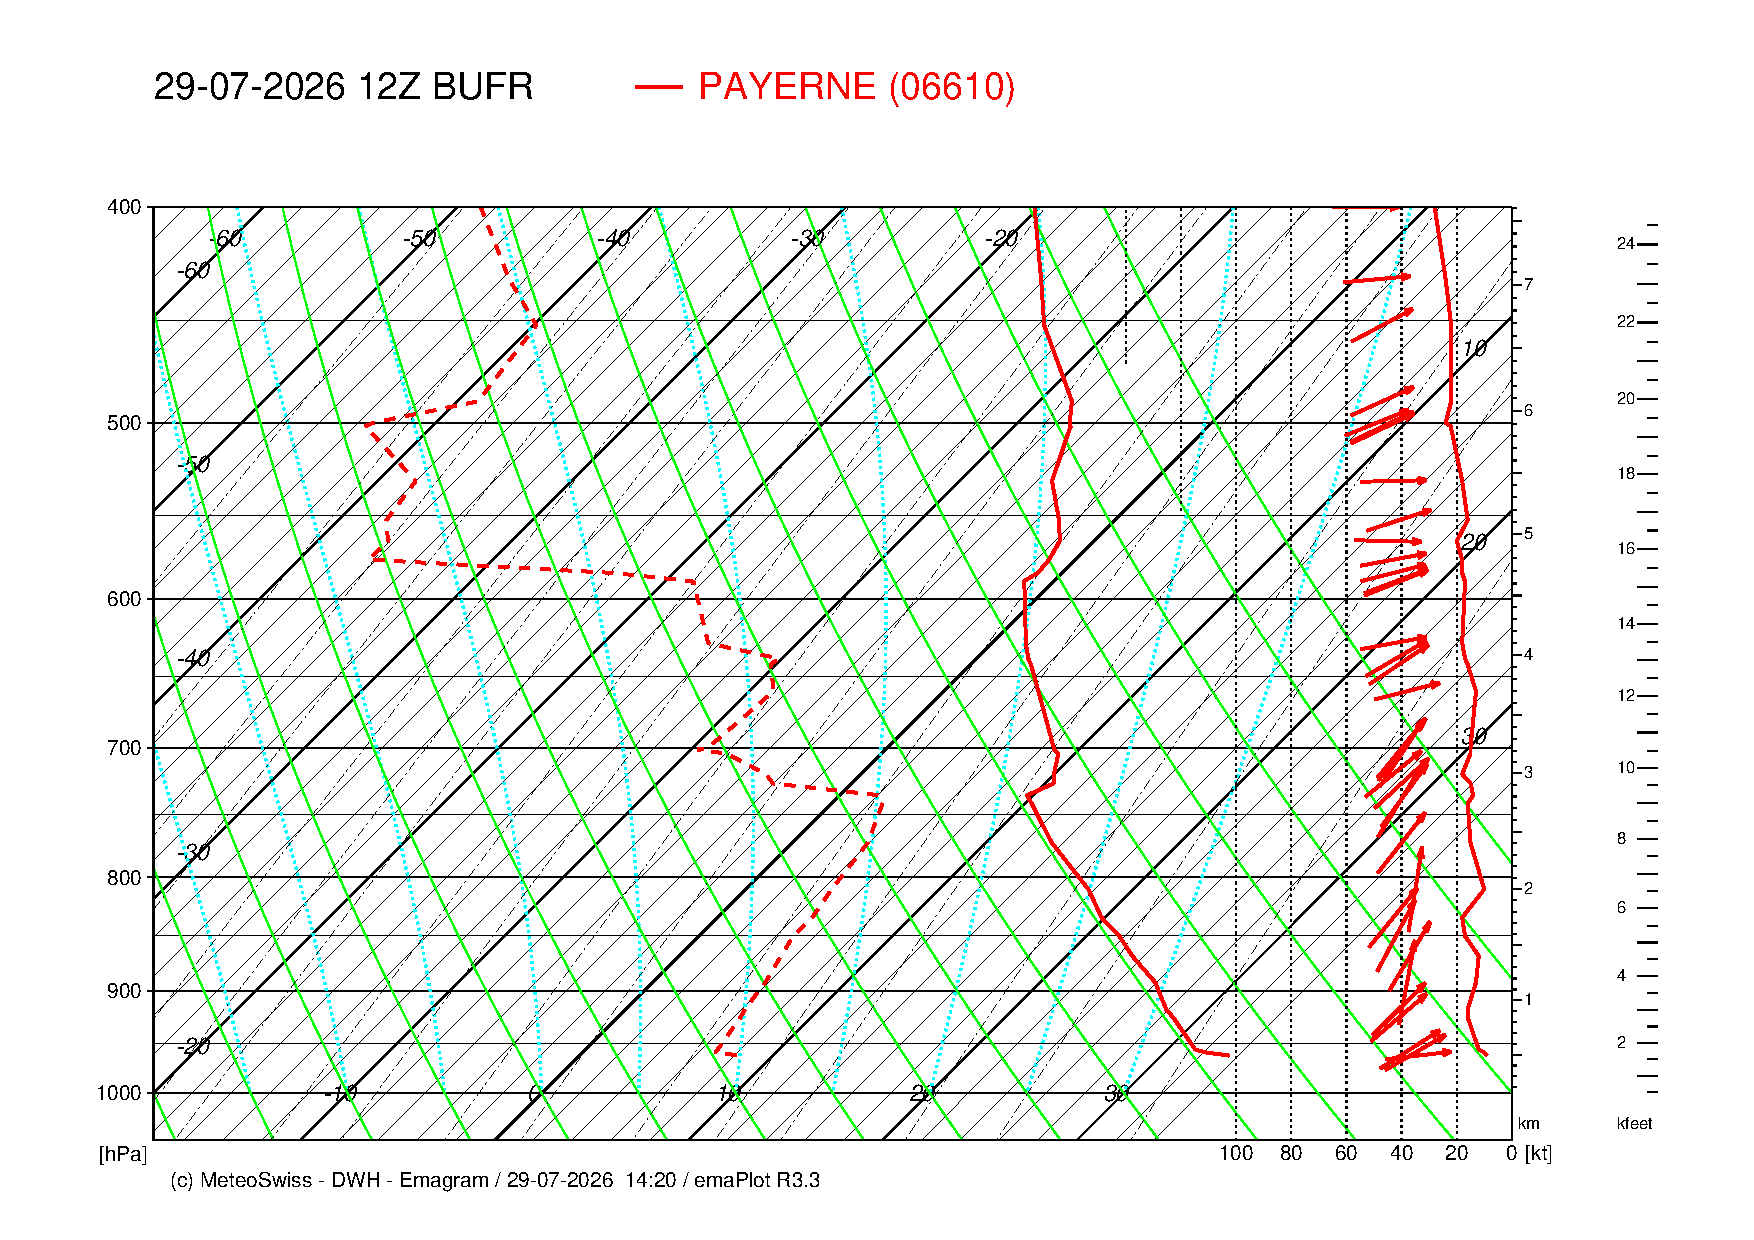
\includegraphics[width=0.8\textwidth]{images/radio-soundings_emagram_payerne.20260729_1200.pdf}

\caption[Emagram of the Payerne radiosounding]{Emagram of the radiosounding at Payerne (station 06610) on 29 July 2026, 12~UTC. Temperature and dew point are plotted against pressure, with the wind profile on the right and height given in both km and kfeet. Copy from MeteoSwiss~\cite{meteoswiss_radiosounding}.}

\label{fig:emagram-payerne}

\end{figure}



Alpine weather and specifically precipitation is also strongly seasonal and diurnal: winter events are predominantly frontal, whereas summer events are largely convective and peak in the afternoon~\cite{nisi2020}. On a typical summer day, a stable layer caps the boundary layer in the morning and suppresses convection. As the sun gradually heats the ground, this stable layer is resolvced. Once it breaks, thermals develop and the convective boundary layer expands to roughly \SIrange{2}{3}{km}; where sufficient convective energy is available, the resulting cumulus clouds grow far beyond that and produce thunderstorms. Whether the cap breaks at all depends on its strength in competition with the heat supplied at the surface, which is why a single daily snapshot of the atmosphere is likely not enough to capture these events.



We aim here to develop a model that can learn the relevant weather processes, rather than provide just accurate predictions. To do that, we try to select a strategic set of input channels that enable the model to learn these relevant processes without the need of hourly data. We therefore include snapshots of the vertical structure of the atmosphere as input, in addition to or as a replacement for surface input. The vertical structure is available from the ERA5 reanalysis of \textcite{hersbach2020era5}, which provides a continuous representation of the atmosphere in the form of curves of temperature, humidity and wind speed against pressure levels\footnote{Low pressure levels represent high altitude layers and high pressure levels are close to the surface.}. These curves are available at every grid point and every hour. To capture the diurnal cycle of convective events, we sample the atmospheric channels at five times of day (00, 06, 12, 15 and 18~UTC), so that the model sees both the capped morning state and the state after the expected breakup, i.e.\ the daily evolution rather than only a daily mean.



Sampling through the day turns a static description of the atmosphere into one that possibly can describe the physical process. \textcite{vaughan2022convcnp} already combine atmospheric with surface channels, but they report neither the timing of those fields nor what each group of channels contributes; \sref{sec:meth-fi} sets out to measure that.


% !TEX root = ../main.tex
% Chapter 3 --- Data
\chapter{Data}\label{ch:data}

In the scope of this work, we use two main data sources. The ERA5 and related datasets provide the coarse-resolution meteorological fields that serve as the model input, while the MeteoSwiss dataset provides the high-resolution measurement data we consider as ground truth for daily maximum temperature and precipitation accumulation. All of them are used over the five years 2020--2024: the models are trained and cross-validated on 2020--2023, and 2024 is held out for the final evaluation (\sref{subsec:meth-cv}). In addition, we use the DHM25 digital elevation model (DEM) to provide the topographical context for the prediction task. The fields used are summarised in \tref{tab:data-grids}. The following sections describe the datasets and the preprocessing steps in more detail.

\begin{table}[htbp]
    \centering
    \caption[Input and target grids]{The two ERA5 input grids~\cite{hersbach2020era5, munozsabater2021era5land} and the MeteoSwiss target grid~\cite{meteoswiss_ogd_grid}.}
    \label{tab:data-grids}
    \footnotesize
    \begin{tabular}{|p{2.2cm}|p{3.5cm}|p{3.5cm}|p{3.5cm}|}
        \hline
        & \textbf{ERA5} & \textbf{ERA5-Land} & \textbf{MeteoSwiss} \\
        \hline
        Product type & Global atmospheric reanalysis: weather model plus observations via data assimilation & Land-surface model rerun forced by ERA5; no data assimilation of its own & Gridded observational analysis, interpolated from the Swiss station network \\
        \hline
        Grid spacing$^{*}$ & $0.25^{\circ} \times 0.25^{\circ}$ (${\sim}19$--$28\,\mathrm{km}$ over Switzerland) & $0.1^{\circ} \times 0.1^{\circ}$ (${\sim}8$--$11\,\mathrm{km}$ over Switzerland) & $1\,\mathrm{km} \times 1\,\mathrm{km}$ on the Swiss LV95 grid.\\
        \hline
        Period / time step & 1940--present, hourly & 1950--present, hourly & TmaxD 1971--, RhiresD 1961--present, daily \\
        \hline
        Fields & Surface and near-surface fields~\cite{era5_single_levels}; upper-air fields on pressure levels~\cite{era5_pressure_levels} & Land and near-surface fields only~\cite{era5land_daily}; no upper-air fields & Daily maximum $2\,\mathrm{m}$ temperature (TmaxD); daily precipitation sum (RhiresD) accumulated from $06\,\mathrm{UTC}$ to $06\,\mathrm{UTC}$\\
        \hline
        Orography handling & Coarse model orography & Daily lapse-rate correction of temperature to the fine-grid elevation; pressure and humidity kept consistent; precipitation inherited from ERA5 & Stations sample the real terrain; interpolation accounts for elevation~\cite{frei2014temperature} \\
        \hline
        Role in this work & Atmospheric input channels: geopotential, temperature, humidity and wind on pressure levels & Surface input channel: daily maximum $2\,\mathrm{m}$ temperature; static geopotential, divided by $g$, for the model orography & Ground truth: training targets and evaluation reference \\
        \hline
    \end{tabular}
    \par\vspace{2pt}
    {\raggedright\scriptsize $^{*}$\,ERA5 and ERA5-Land use regular latitude--longitude grids, so their grid spacing in km varies with latitude.\par}
\end{table}

\section{Meteorological Model Inputs: ERA5}\label{sec:data-era5}

ERA5 is a global meteorological reanalysis product produced by the European Centre for Medium-Range Weather Forecasts (ECMWF)~\cite{hersbach2020era5}. It combines a numerical weather model with observations through data assimilation to give a physically consistent record of the atmosphere. We access it through the Copernicus Climate Data Store (CDS).

ERA5-Land is the land-surface reanalysis derived from ERA5~\cite{munozsabater2021era5land, era5land_daily}. It is produced by running ECMWF's land-surface model on its own, controlled by the near-surface fields of ERA5, on a finer grid. To force the land model on the finer grid, the ERA5 fields are first interpolated horizontally to $0.1^{\circ}$.  The refined surface temperature is then corrected to the true elevation of each fine cell.

Temperature varies with altitude in a well-defined way; this correction recovers part of the mountain and valley structure that the coarse ERA5 grid averages away. This correction applies only to the thermodynamic fields; however, precipitation is taken over from ERA5 as forcing and gains no real sub-grid detail beyond the interpolation to the finer grid.

\section{MeteoSwiss Targets: Temperature and Precipitation}\label{sec:data-targets}

The MeteoSwiss dataset provides the high-resolution measurement data we consider as ground truth for daily maximum temperature and precipitation accumulation. We use the gridded products TmaxD for temperature and RhiresD for precipitation~\cite{meteoswiss_ogd_grid}. Both are derived from the MeteoSwiss station network by spatial interpolation \cite{frei2014temperature,frei1998precip} and are provided on a regular $1\,\mathrm{km} \times 1\,\mathrm{km}$ grid in the Swiss LV95 coordinate system, at a temporal resolution of one day. Note that the $1\,\mathrm{km}$ grid spacing overstates the real information content: the effective resolution is limited by the density of the station network.

The precipitation target is not a calendar-day total. RhiresD accumulates from $06\,\mathrm{UTC}$ to $06\,\mathrm{UTC}$ of the following day, and the value carries the date of the day on which the accumulation begins~\cite{meteoswiss_rhiresd_doc}. The ERA5 input day is the UTC calendar day, so the target day and the input day do not cover the same twenty-four hours; the offset is quantified in \sref{subsec:data-coords}. The two roles ERA5-Land plays are therefore kept strictly apart. As a model \emph{input} channel it enters as the UTC calendar-day total, accumulated $00$--$00\,\mathrm{UTC}$, and the six-hour offset against the target is part of what the model has to work around. As the \emph{evaluation reference} it is re-accumulated over the same $06$--$06\,\mathrm{UTC}$ window as RhiresD, so that reference and target cover the same twenty-four hours and the skill scores of \cref{ch:single-model} compare like with like (\sref{subsec:app-skill-precip}).

\section{Topography (DHM25): DEM and TPI}\label{sec:data-topography}

High-resolution topography for this project has been prepared by the predecessor project of \textcite{passos}; no modifications have been made within this project. The height data is derived from the $25\,\mathrm{m}$ swisstopo DHM25 digital height model (DEM), described by \textcite{swisstopo_dhm25}, and is stored on a regular $50\,\mathrm{m}$ grid in the Swiss LV95 coordinate system. It provides the elevation MLP with the local elevation, the elevation difference to the coarse input grid, and the topographic position index at a $500\,\mathrm{m}$ scale (TPI-500\footnote{The topographic position index compares the elevation of each point with the mean elevation of the surrounding terrain within a given radius, here $500\,\mathrm{m}$: positive values mark ridges and hilltops, negative values valleys, and values near zero flat ground or uniform slopes, following \textcite{weiss2001tpi}.}). The MeteoSwiss target coordinates are given in WGS84, so we transform them to LV95 and bilinearly interpolate the topographic fields at each $1\,\mathrm{km}$ target point.

\section{Preprocessing and Features}\label{sec:data-preprocessing}

\subsection{Coordinate Alignment and Normalisation}\label{subsec:data-coords}
The three datasets have different coordinate systems and grid resolutions, so they need to be aligned and normalised before they can be used together. \textcite{passos} established a workflow to align the MeteoSwiss target points with the ERA5-Land surface field. We keep the core approach, but to provide compatibility with the atmospheric input, some adjustments were necessary and are described below.

One point governs everything that follows: the datasets are never projected onto a single common grid. Two frames coexist by design. The \emph{encoder grid} is a regular latitude--longitude lattice and carries the input channels; the \emph{target points} are the MeteoSwiss locations, handled as an unstructured list of coordinates rather than as a lattice. The only link between them is the squared-distance matrix of step~\ref{item:data-grid-geometry}, which the final layer turns into an interpolation kernel. What is shared is the domain: the ERA5-Land $0.1^{\circ}$ field is loaded first, and its bounding box fixes the latitude and longitude range against which every coordinate in the pipeline, on either side, is normalised.

In practice, every coordinate system gets reprojected onto the shared WGS84 domain above, the encoder grid is picked for whichever configuration is running (the native ERA5-Land or ERA5 lattice), the DHM25 topography is looked up at each target point, and the distance matrix the RBF layer needs is built from there. Each field is then normalised in whatever way fits it: weather channels and the temperature target are $z$-scored, coordinate and seasonal channels are already bounded so they are left as they are, and precipitation stays in raw millimetres so the exact zeros the Bernoulli--Gamma head needs are not shifted away from zero. All of these normalisation numbers are saved with the trained model, so new data is normalised the same way later on. The full step-by-step version, including the exact order of operations and the six-hour offset between the UTC-day input and the precipitation target's accumulation window, is in \sref{sec:app-preprocessing}.

\tref{tab:data-context} lists the composition of each configuration and the stage
at which every input enters the architecture; \fref{fig:input-channels} shows the
surface and atmospheric sets in detail.

\begin{table}[htbp]
    \centering
    \caption[Model inputs and where they enter]{Inputs to the model and the stage at which they enter. The upper block gives the encoder context for the configurations compared in this work, where the scaffold denotes the two coordinate channels, the two seasonal channels and the elevation channel. The lower block gives the remaining inputs, which are the same in every configuration. $P$ is the number of target points and $B$ the number of days in a batch. The pressure-level variables are given by their ERA5 short names: $z$ geopotential, $t$ temperature, $q$ specific humidity, $u$ and $v$ the eastward and northward wind components. The surface field of the ERA5-Land configurations is $\mathrm{t2m\_max}$, the daily maximum $2\,\mathrm{m}$ temperature; the surface precipitation configuration adds $\mathrm{tp}$, the daily precipitation total; the two surface anchors of the atmospheric configuration are $\mathrm{t2m}$, the $2\,\mathrm{m}$ temperature, and $\mathrm{tp}$, the total precipitation. The six levels are $1000$, $925$, $850$, $700$, $500$ and $300\,\mathrm{hPa}$, and the five hours are $00$, $06$, $12$, $15$ and $18$ UTC.}
    \label{tab:data-context}
    \footnotesize
    \begin{tabular}{|p{3.2cm}|p{2.8cm}|p{4.6cm}|p{2.1cm}|}
        \hline
        \textbf{Input} & \textbf{Entry Point} & \textbf{Content} & \textbf{Dimension} \\
        \hline
        \multicolumn{4}{|l|}{\textit{Encoder context: one tensor per day, assembled as described above}} \\
        \hline
        Surface --- baseline & Encoder, ERA5-Land $0.1^{\circ}$ & $\mathrm{t2m\_max}$ + scaffold & 6 channels \\
        \hline
        Surface without elevation$^{*}$ & Encoder, ERA5-Land $0.1^{\circ}$ & $\mathrm{t2m\_max}$ + scaffold without the elevation channel & 5 channels \\
        \hline
        Surface precipitation & Encoder, ERA5-Land $0.1^{\circ}$ & $\mathrm{tp}$ + $\mathrm{t2m\_max}$ + scaffold & 7 channels \\
        \hline
        Atmospheric & Encoder, ERA5 $0.25^{\circ}$ & 3 variables ($z$, $t$, $q$) $\times$ 6 levels $\times$ 5 hours + scaffold & 95 channels \\
        \hline
        Atmospheric with surface anchors & Encoder, ERA5 $0.25^{\circ}$ & 3 variables ($z$, $t$, $q$) $\times$ 6 levels $\times$ 5 hours + $\mathrm{t2m}$ and $\mathrm{tp}$ $\times$ 5 hours + scaffold & 105 channels \\
        \hline
        Atmospheric with wind & Encoder, ERA5 $0.25^{\circ}$ & 5 variables ($z$, $t$, $q$, $u$, $v$) $\times$ 6 levels $\times$ 5 hours + scaffold & 155 channels \\
        \hline
        \multicolumn{4}{|l|}{\textit{Further inputs: identical in every configuration}} \\
        \hline
        Distance matrix & Final layer & Squared distance in degrees from every target point to every point of the input grid & $(P, \mathrm{lat}, \mathrm{lon})$ \\
        \hline
        Topographic features & Elevation MLP & Elevation, difference to the model orography, TPI-500 & $(P, 3)$ \\
        \hline
        Seasonal features & Elevation MLP & $\cos$ and $\sin$ of the day of year, also present as two context channels & $(B, 2)$ \\
        \hline
    \end{tabular}
    \par\vspace{2pt}
    {\raggedright\scriptsize $^{*}$\,These five channels are exactly the encoder context of the predecessor project of \textcite{passos}, which passed the surface temperature, the two coordinates, and the two seasonal channels to the encoder and kept all elevation information in the elevation MLP. Of the configurations studied here, this one is therefore the closest in methodology to that work.\par}
\end{table}

\begin{figure}[H]
    \centering
    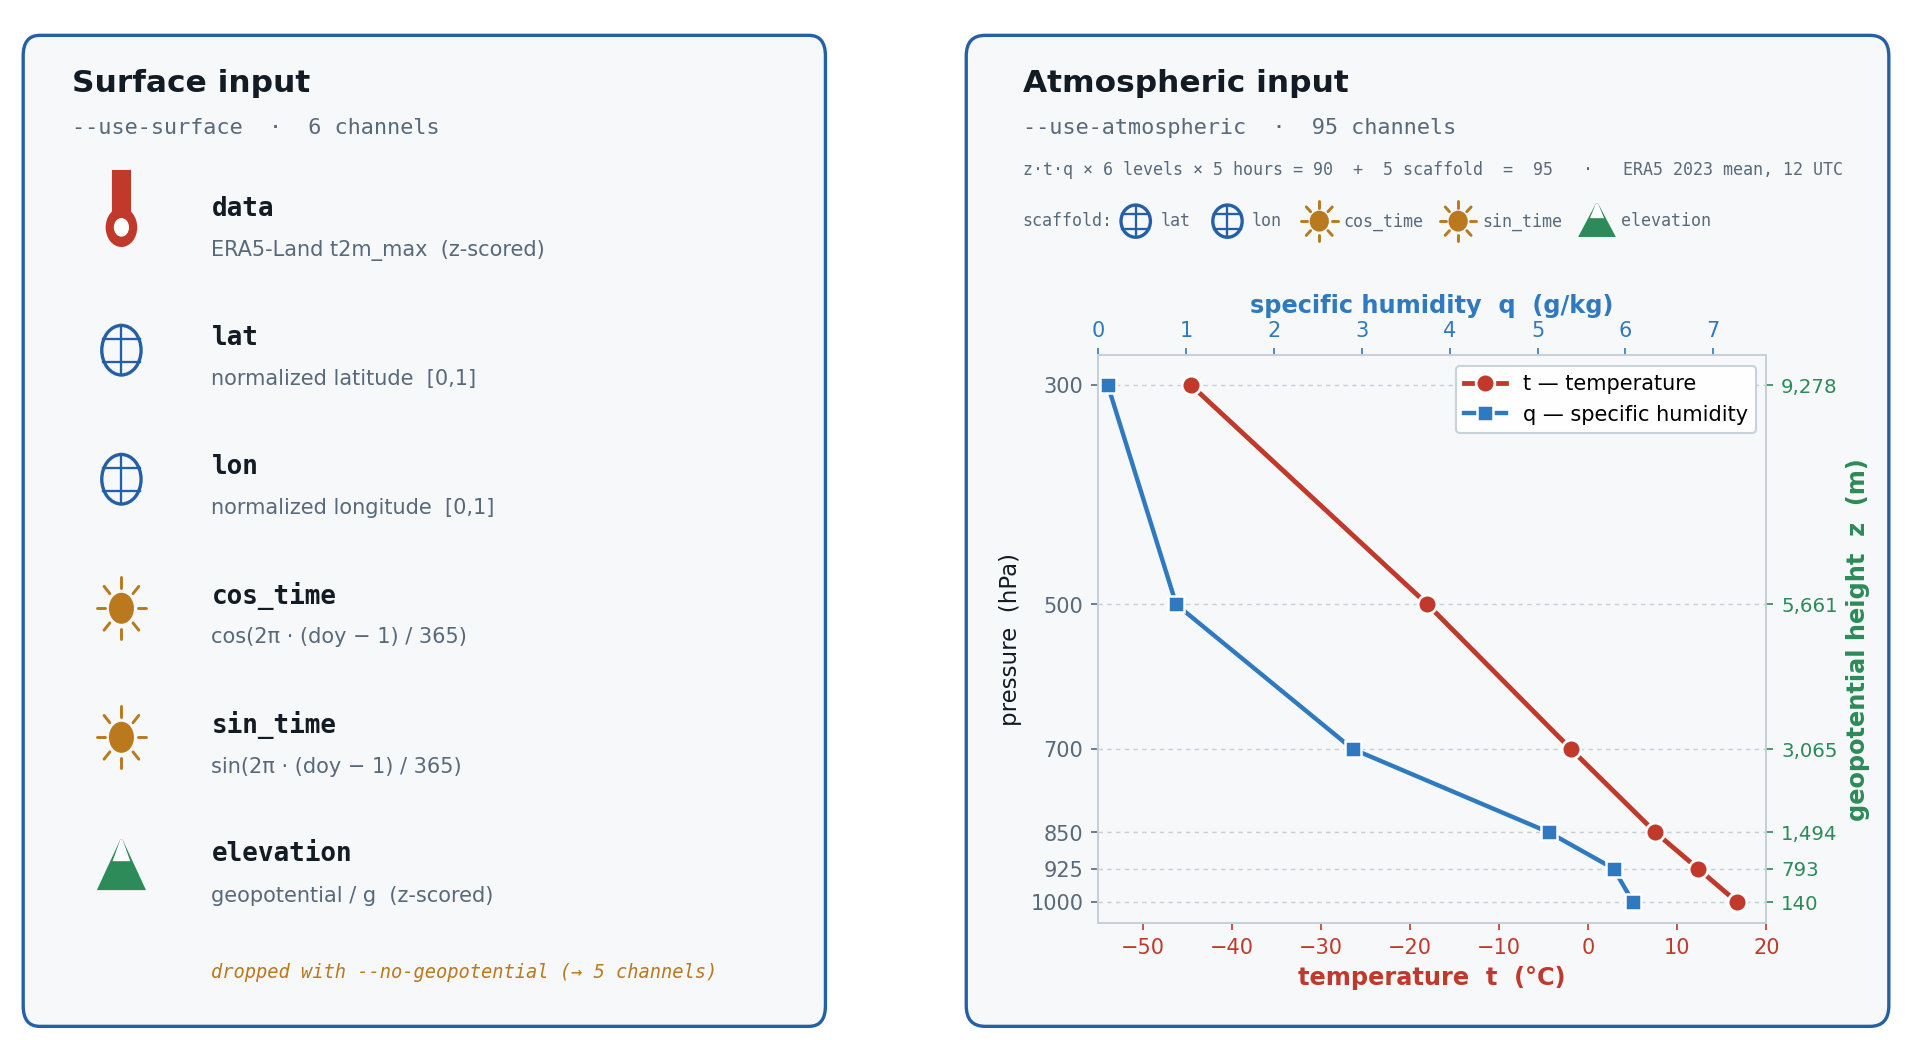
\includegraphics[width=0.9\textwidth]{images/12_input_channels.png}
    \caption[The surface and atmospheric input channel sets]{The two input channel sets of \tref{tab:data-context} in detail. Left: the six surface channels with their normalisation. Right: the atmospheric set, where geopotential, temperature and specific humidity are taken at six pressure levels and five times of day ($90$ channels), plus the same five scaffold channels, giving $95$. Wind components enter only in the extended atmospheric configuration. The emagram marks the six pressure levels on the domain-mean ERA5 profile for 2023 at 12~UTC, with geopotential height on the right-hand axis.}
    \label{fig:input-channels}
\end{figure}

\subsection{Differences to the Predecessor Project}\label{subsec:data-predecessor}

Three points depart from the inherited pipeline.
\begin{itemize}
    \item \textbf{Alignment of the input grid} Every file's coordinates are snapped to five decimals before the yearly ERA5 files are merged, since ERA5 stores the same grid line with a drift of about $10^{-13}$ degrees between files. Five decimals is about a metre on the ground, far finer than the $0.1^{\circ}$ spacing of the grid and far coarser than the drift, so the snap moves no grid cell and the files merge onto one common lattice.
    \item \textbf{Normalisation statistics} The predecessor normalised a single surface field with statistics recomputed from whatever data was being loaded, and stored only those two numbers. In this work, we follow the principle that every channel needs its own statistics, and they must be stored with the model, or a model applied to a new year is normalised differently than it was trained. Within the same rework, we made the target normalisation configurable, so precipitation stays in millimetres while temperature is standardised.
    \item \textbf{Elevation input channel} In the predecessor project, elevation reached the model only through the elevation MLP, never as an input channel to the encoder. This was not a deliberate choice, but a code bug discovered late in the project. Here the geopotential-derived elevation channel is part of the input context unless stated otherwise.
\end{itemize}

Taken together, these differences mean that results obtained with the earlier pipeline are not a suitable baseline for our work. We therefore treat the predecessor project as the starting point of this implementation rather than as a benchmark, and rerun the surface configuration under the corrected pipeline to obtain our own baseline. As an external reference, we use, if applicable, the published results of \textcite{vaughan2022convcnp}, who introduced the downscaling approach we follow here. All comparisons reported below are made against one of these two references (\cref{ch:single-model}).


% !TEX root = ../main.tex
\chapter{Methodology}\label{ch:methodology}

\section{ConvCNP Architecture}\label{sec:meth-architecture}
The architecture of the ConvCNP model, adapted from \textcite{vaughan2022convcnp}, is presented in \fref{fig:meth-architecture}.
The model consists of a convolutional encoder that processes the input context channels and learns the contextual relationship, followed by a CNN backbone with an RBF final layer that learns the spatial relationship between the input grid and the target points. The model is completed by an elevation MLP that corrects the predictive distribution parameters for terrain effects. The architecture is the same for both temperature and precipitation, with the only difference being the number of input channels and the output distribution. Written as a single expression, the parameters $\theta$ of the predictive distribution at a target point $x$ are
\begin{equation}
    \theta(x) \;=\; \mathrm{MLP}_{\mathrm{elev}}\Bigl[\,\varphi_{\ell}\bigl(\mathrm{MLP}_{\mathrm{par}}(\mathrm{CNN}(\mathrm{Enc}(Z))),\; x\bigr),\;\, e(x),\;\, s \,\Bigr],
\label{eq:convcnp-composition}
\end{equation}
where $Z$ is the context tensor on the input grid, $e(x)$ the terrain features at the target point, $s$ the seasonal encoding, and $\varphi_{\ell}$ the RBF interpolation of \eref{eq:rbf-interp}. The following subsections provide further detail on the individual model components.
\begin{figure}[H]
\centering
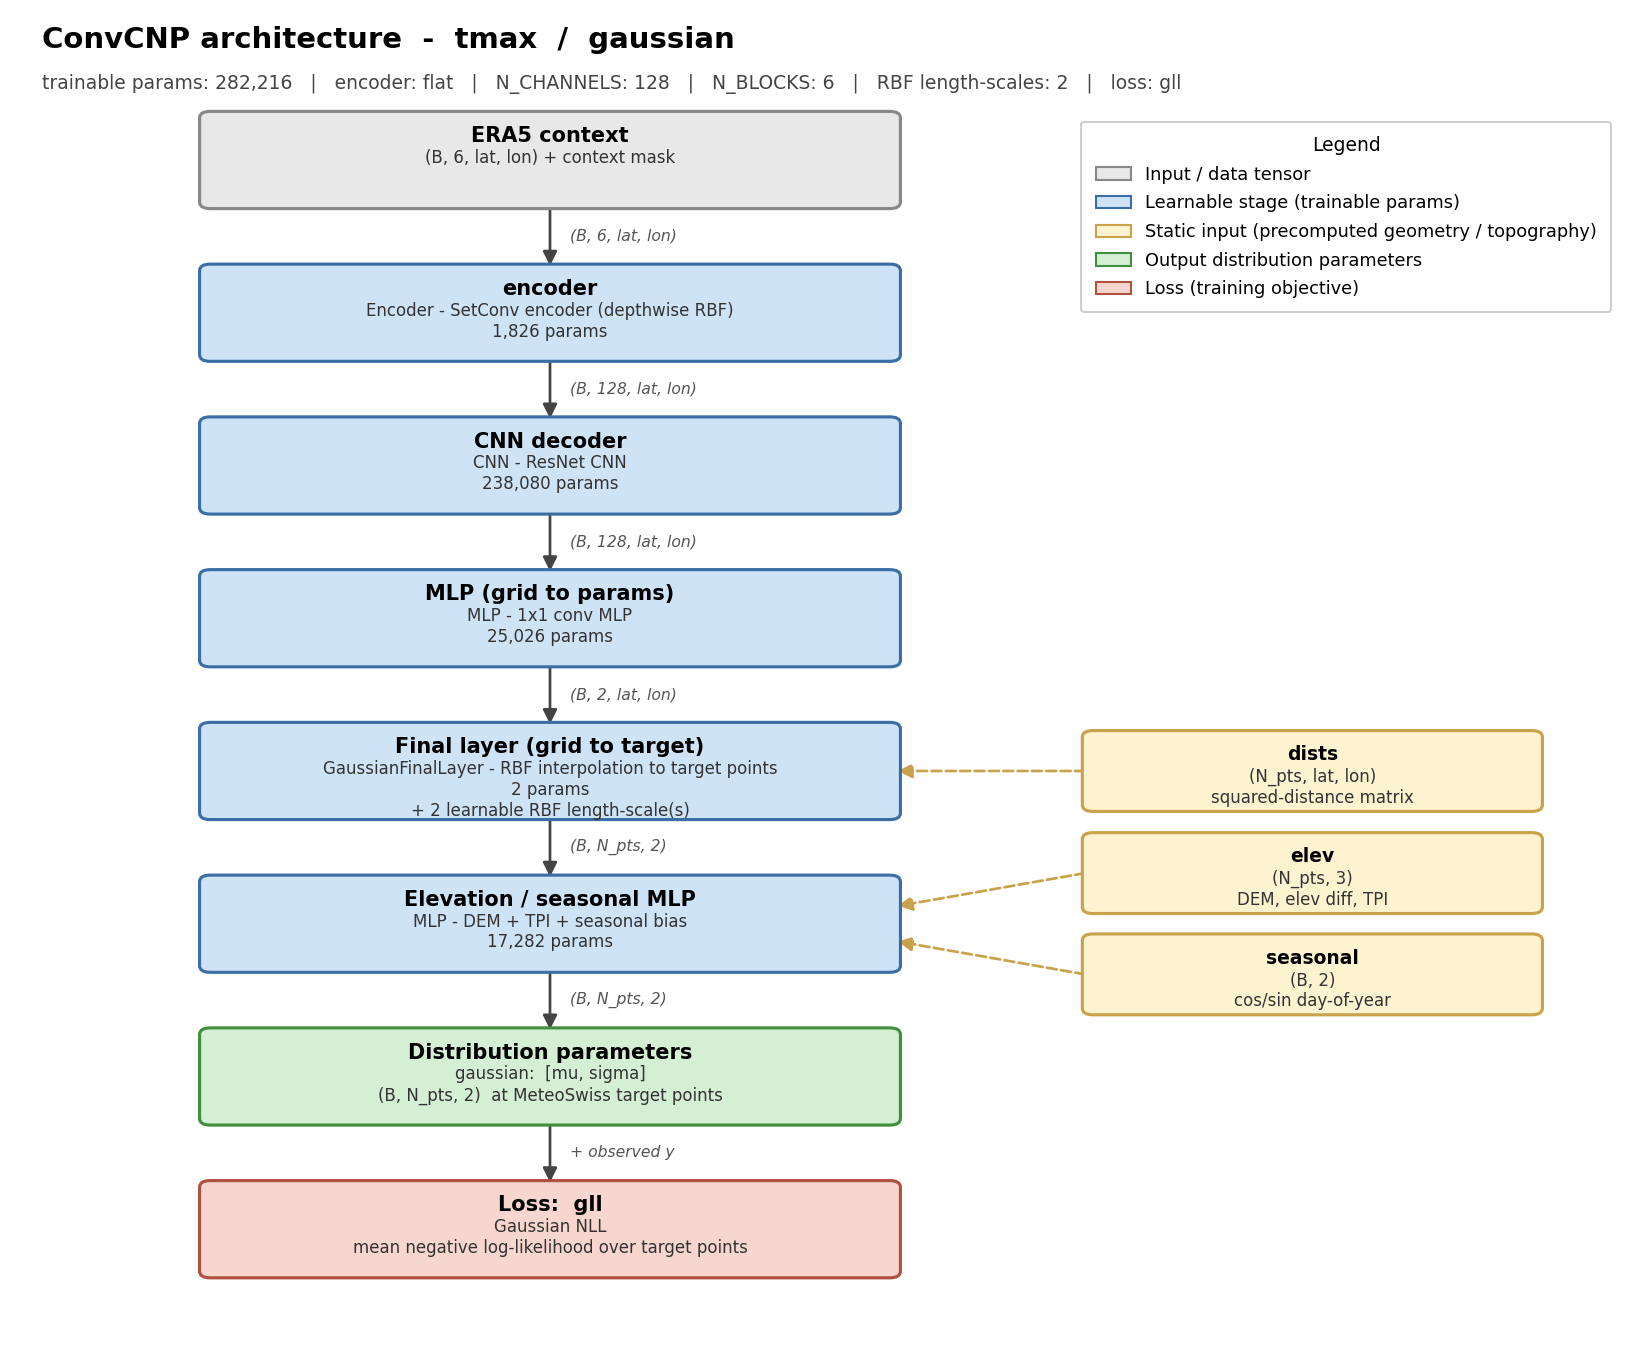
\includegraphics[width=0.45\textheight]{images/architecture/tmax-surface_architecture.png}
\caption[ConvCNP architecture of the surface-baseline model]{ConvCNP architecture for the surface-baseline temperature model (\tref{tab:data-context}). Atmospheric configurations differ only in the number of encoder input channels and the input grid resolution. The temperature and precipitation models differ depending on their configuration in the predictive distribution and the objective function.}
\label{fig:meth-architecture}
\end{figure}

\subsection{Encoder, CNN Processor, and RBF Final Layer}\label{subsec:meth-backbone}
In this part of the architecture, the model learns the relationships between the input channels and how to map them to the target points. The encoder processes the input context channels, which are stacked into a tensor $Z$ on their native grid. This tensor passes through the encoder, a depthwise set convolution that normalises each channel by its observation density, followed by a linear layer that lifts the channels to the working width of the CNN. The CNN backbone is a ResNet that learns the meteorological and spatial structure of the fields on the input grid. To simplify the use of different predictive distributions, the output distribution parameters are generated in a separate layer (MLP (grid to params)). The distribution parameters are then passed to a final layer that maps them from the input grid to the target points using RBF interpolation.

The RBF interpolation layer lets the model predict at arbitrary target points rather than only on the input grid. That is what downscaling needs, since the fine target locations do not align with the coarse lattice, and it is also what allows the model to be queried directly at station coordinates, as in \textcite{vaughan2022convcnp} or in \cref{ch:stations}.
The model learns for each parameter $k$ of the distribution (for example $\mu, \sigma$ for the Gaussian) its own length scale $\ell_k$ for the RBF kernel that is used to interpolate in 2D space the parameters from the input grid to the target points,
\begin{equation}
    \tilde{\theta}_k(x) \;=\; \sum_{i,j} h_k(g_{ij})\, \exp\!\left(-\frac{\lVert x - g_{ij} \rVert^{2}}{2\,\ell_k^{2}}\right),
\label{eq:rbf-interp}
\end{equation}
where $g_{ij}$ are the points of the input grid and $h_k(g_{ij})$ the gridded value of parameter $k$ produced by the previous layer. The target location $x$ enters only through its distance to the grid points, so the layer is tied to no fixed set of target locations and can be queried anywhere in the domain. Its output $\tilde{\theta}_k(x)$ is defined at the target points, but is still a smooth interpolation of the coarse field; the sub-grid terrain detail is added by the elevation MLP.
The calculation of the RBF kernel is a huge task because of the high number of target points and grid cells. To avoid memory issues within the GPU, the RBF kernel has to be  evaluated in chunks.

\subsection{Elevation MLP Correction}\label{subsec:meth-elev-mlp}

The elevation MLP, $\mathrm{MLP}_{\mathrm{elev}}$ in \eref{eq:convcnp-composition}, is used to add the terrain information to the model. The elevation MLP is a small MLP that takes the current distribution parameters together with the terrain features of the target points (elevation, elevation difference to the coarse model orography, TPI-500; \tref{tab:data-context}) together with the seasonal encoding, and outputs the corrected parameters of the predictive distribution directly,
\begin{equation}
    \theta(x) \;=\; \mathrm{MLP}_{\mathrm{elev}}\bigl(\,\tilde{\theta}(x) \oplus e(x) \oplus s\,\bigr),
\label{eq:elev-mlp}
\end{equation}
where $\oplus$ denotes concatenation: the three terrain features $e(x)$ and the two seasonal values $s$ are appended to the parameters $\tilde{\theta}(x)$ coming from \eref{eq:rbf-interp}. This gives seven inputs for temperature and eight for precipitation. The MLP returns a complete representative set of parameters, not merely an offset or bias added to $\tilde{\theta}(x)$.

This lets the model correct predictions that would otherwise be elevation agnostic, following \textcite{vaughan2022convcnp}, including seasonal effects such as differing lapse rates between summer and winter. Both the terrain and the seasonal encoding reach the model twice: coarsely, as scaffold channels processed by the encoder--CNN chain, and per target point, through the elevation MLP. This creates the link between the elevation seen for the meteorological input and the fine-grained per-point features including true elevation, TPI-500 and the elevation difference to the coarse model orography.

\section{Output Distributions}\label{sec:meth-distributions}

We study two separate target variables that behave differently. Daily maximum temperature at $2\,\mathrm{m}$ above ground is a continuous variable that is well modelled by a Gaussian distribution. Daily precipitation accumulation is more complex, as most days are dry and the wet days follow a skewed distribution. A Bernoulli--Gamma mixture is the standard parametric answer, used for precipitation density networks by \textcite{cannon2008berngamma} and for ConvCNP downscaling by \textcite{vaughan2022convcnp}; we adopt it here.

For both variables the model predicts the parameters of a distribution at each target point and day rather than a single value. Downscaling is ill-posed, one coarse field being compatible with many fine-scale outcomes, and a distribution keeps that ambiguity explicit; it also makes the probability of exceeding any threshold directly available and lets the prediction be checked for calibration.

Each distribution is factorised across target points (\sref{sec:bg-neural-processes}): \eref{eq:gauss-density} and \eref{eq:bg-density} are marginals at one point and day, not components of a joint distribution with a learned covariance. The predicted spread therefore describes that point alone and says nothing about its neighbours, and every score of \sref{subsec:meth-metrics} is accordingly a marginal score.

\subsection{Gaussian for Temperature}\label{subsec:meth-gaussian}

For temperature, this distribution is a Gaussian: the model outputs a mean $\mu$ and a standard deviation $\sigma$ at every target point, which define the density over the possible temperatures $y$,
\begin{equation}
    p(y) \;=\; \frac{1}{\sqrt{2\pi\sigma^{2}}} \exp\!\left(-\frac{(y - \mu)^{2}}{2\sigma^{2}}\right).
\label{eq:gauss-density}
\end{equation}
\fref{fig:meth-tmax-dist} illustrates the resulting density: one mean and one spread per target point and day.

\begin{figure}[H]
\centering
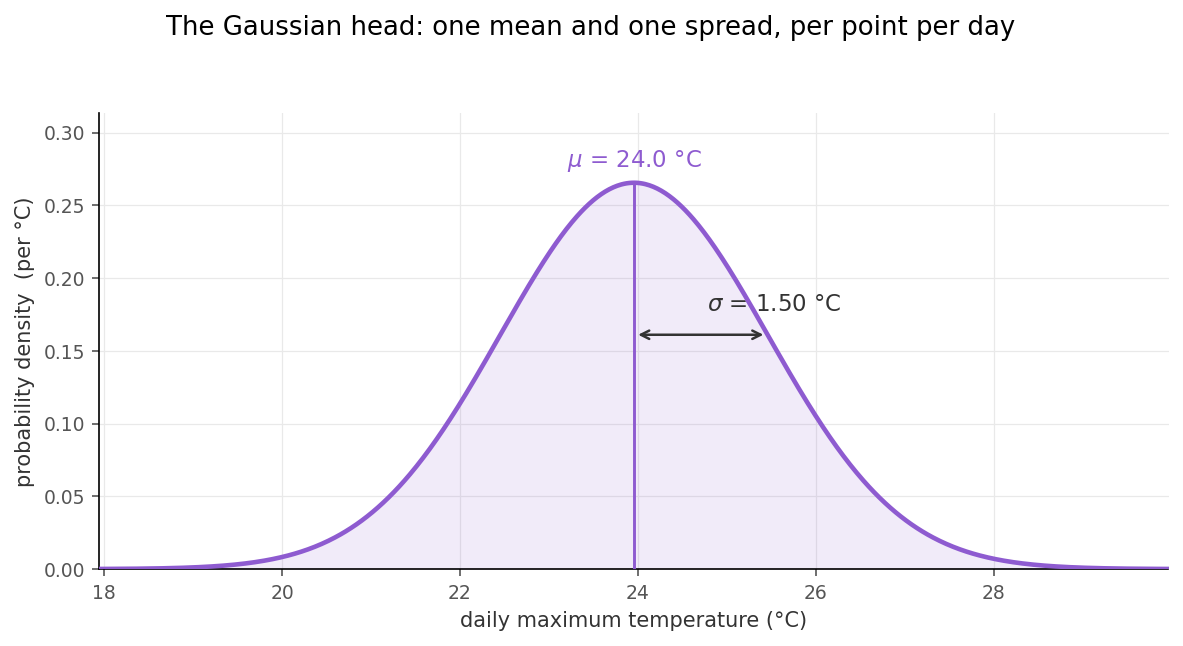
\includegraphics[width=0.9\textwidth]{images/16_tmax_distribution.png}
\caption[The Gaussian predictive distribution]{The Gaussian predictive density for a single target point and day. The model outputs the two parameters: the mean $\mu$ locates the distribution and the standard deviation $\sigma$ sets its width, shown here for $\mu = 24.0\,^{\circ}\mathrm{C}$ and $\sigma = 1.5\,^{\circ}\mathrm{C}$.}
\label{fig:meth-tmax-dist}
\end{figure}
\subsection{Bernoulli--Gamma for Precipitation}\label{subsec:meth-likelihoods}

Precipitation needs a different shape. Most days are exactly dry, $0\,\mathrm{mm}$, and the wet days follow a skewed, strictly positive distribution (\sref{subsec:data-coords}). Following \textcite{cannon2008berngamma} and \textcite{vaughan2022convcnp}, we therefore use a Bernoulli--Gamma mixture: $\rho$ is the probability that the day is wet, and $\alpha$ and $\beta$ are the shape and rate of a Gamma distribution for the amount of precipitation. Write $g(y; \alpha, \beta)$ for that Gamma density and $G(y; \alpha, \beta)$ for its cumulative distribution function. A wet day is scored by the probability of rain times the density of the amount, a dry day by the probability of staying dry,
\begin{equation}
    p(y) \;=\;
    \begin{cases}
        \rho \, g(y; \alpha, \beta) & y > 0 \text{ (wet)}, \\
        1 - \rho & y = 0 \text{ (dry)}.
    \end{cases}
\label{eq:bg-density}
\end{equation}
The three parameters are easiest to read as the probability of at least $t$ millimetres. For any threshold $t > 0$ the mixture of \eref{eq:bg-density} gives that probability in closed form,
\begin{equation}
    P(Y \geq t) \;=\; \rho \, \bigl(1 - G(t; \alpha, \beta)\bigr),
\label{eq:bg-exceedance}
\end{equation}
which reads directly: the day has to be wet, which costs $\rho$, and the amount then has to reach $t$. This exceedance probability is what the precipitation indices and skill scores later ask of the model (\sref{subsec:app-skill-precip}). \fref{fig:meth-precip-dials} visualises different shapes of possible output distributions. $\rho$ reweights the same wet body without changing its shape such that the gap to 1 at 0 mm is the probability of a dry day. $\beta$ changes how much precipitation accumulates once it does rain, stretching the curve to the right while the dry mass stays where it is. $\alpha$ changes the shape of a wet day: a given average is reached either through many small amounts or through fewer, heavier ones. The provided examples are realistic draws from a model output.

\begin{figure}[H]
\centering
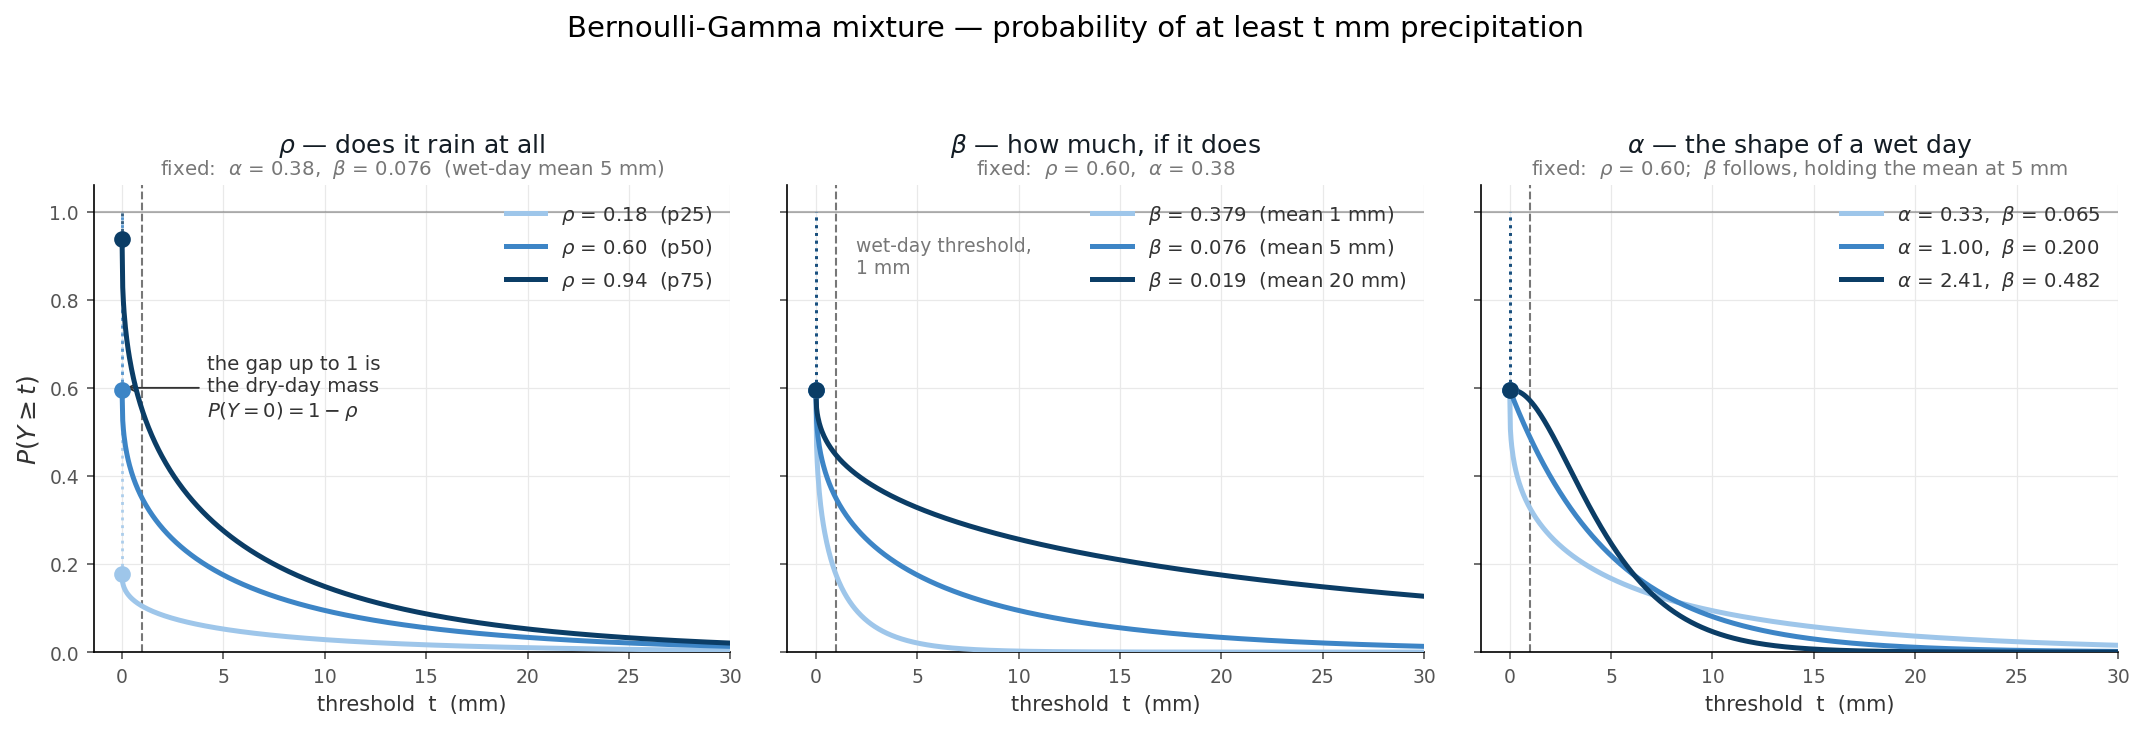
\includegraphics[width=\textwidth]{images/17_precip_wet_dry_day.png}
\caption[Bernoulli--Gamma distribution]{The Bernoulli--Gamma head read as the probability of at least $t$ millimetres, with one parameter turned per panel and the other two held constant. All parameter values are sampled from one of the model own outputs}

\label{fig:meth-precip-dials}
\end{figure}

\fref{fig:meth-precip-dials} reads the distribution at a single point and day; \sref{subsec:app-skill-precip} explains how these point-day distributions are pooled into the frequencies the results chapter actually reports.

\section{Training and Evaluation Setup}\label{sec:meth-training}

\subsection{Temporal $k$-Fold Cross-Validation and Hyperparameters}\label{subsec:meth-cv}

The models of this work are trained on the four years 2020--2023 and never see the year 2024, which is kept aside for the final evaluation. Within the training years, we use a temporal $k$-fold cross-validation with $k=5$: the days are split into five contiguous blocks of about $290$ days, and each fold trains on four blocks while the fifth is held out (\fref{fig:meth-cv-scheme}). The blocks are contiguous in time on purpose. Consecutive days share their weather, so a random split would place near-copies of training days into the held-out set and overstate the skill; a held-out block of many consecutive months has to be predicted from genuinely different periods.

\begin{figure}[H]
\centering
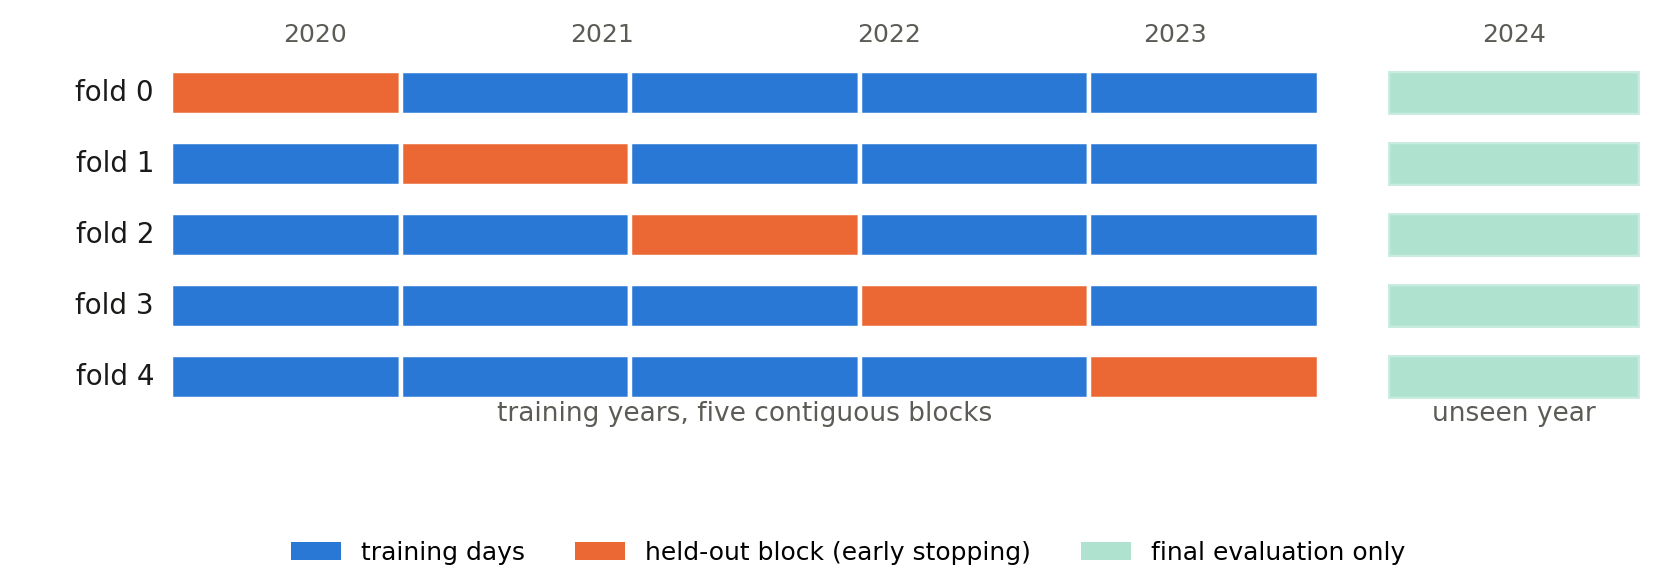
\includegraphics[width=0.9\textwidth]{images/cv_scheme.png}
\caption[Temporal cross-validation scheme]{The temporal $5$-fold scheme. Each fold trains on four contiguous blocks of 2020--2023 and holds out the fifth; the year 2024 is used for the final evaluation only.}
\label{fig:meth-cv-scheme}
\end{figure}

The training loop is standardised, and the hyperparameters it uses are collected in
\tref{tab:meth-training-setup}. They follow \textcite{vaughan2022convcnp} and the predecessor
pipeline rather than a tuning study of their own; beyond an early coarse screen of the
precipitation model, no hyperparameter search was run in this work.

The loop is identical for both variables; only the objective differs, and with it the stabilisation it needs, as the two subsections below state.


The five-fold split of \fref{fig:meth-cv-scheme} creates two deployment regimes: in the cross-validation evaluation each model predicts only the holdout block it never trained on, so every day is predicted exactly once by an independent model, whereas in all inference situation on unseen data the five trained models act together as an ensemble (\sref{sec:meth-inference}).

\subsection{Objective Functions}\label{objective}
The negative log-likelihood objectives follow \textcite{vaughan2022convcnp}. For the precipitation model, we extended the training with a CRPS-based objective function, used both from scratch and as a fine-tune of a converged likelihood model. The fine-tune is what earns the third run its place: ten of its epochs recover more of the held-out CRPS than thirty epochs of training on the CRPS from scratch (\sref{sec:app-precip-training}).

Whichever objective is used, it is evaluated over the Swiss domain alone. The input grid extends beyond the national border (\tref{tab:data-context}), but the loss is formed only at the MeteoSwiss target points that carry an observation: target values outside the analysis domain are missing, and every objective drops them before averaging. Of the $88\,800$ points of the temperature lattice, $46\,718$ ($53\,\%$) are inside Switzerland and enter the loss; the precipitation lattice contributes about $64\,\%$ of its $98\,050$ points. The exclusion happens at the loss and nowhere earlier. The context grid is never cropped, the full rectangular MeteoSwiss product grid is flattened into the target-point tensor with the outside-Switzerland points kept as \texttt{NaN} rather than removed, and the model's forward pass, the RBF final layer and the elevation MLP alike, predicts at every one of those points, including the ones with no observation. 
\subsubsection*{Temperature}\label{subsubsec:meth-train-tmax}

The temperature runs minimise the negative log-likelihood of the Gaussian of \eref{eq:gauss-density}, averaged over all target points and days of a batch,
\begin{equation}
    \mathcal{L}_{\mathrm{T}} \;=\; -\,\overline{\log p(y)} \;=\; \overline{\tfrac{1}{2}\log\bigl(2\pi\sigma^{2}\bigr) + \frac{(y - \mu)^{2}}{2\sigma^{2}}}.
\label{eq:gauss-ll}
\end{equation}
The targets enter in normalised units, $z$-scored with the statistics of the ERA5-Land $\mathrm{t2m\_max}$ field (\sref{subsec:data-coords}), so the objective sees values of order one. The Gaussian likelihood is well behaved throughout, and no further stabilisation is needed.

\subsubsection*{Precipitation}\label{subsubsec:meth-train-precip}

The precipitation runs train on raw millimetres: a $z$-score would push the exact zeros to negative values and destroy the point mass the Bernoulli--Gamma mixture is built on (\sref{subsec:data-coords}).

Two objectives are implemented and selected per run. The first is the negative log-likelihood of the mixture of \eref{eq:bg-density},
\begin{equation}
    \mathcal{L}_{\mathrm{P}} \;=\; -\,\overline{r\,\bigl(\log \rho + \log g(y; \alpha, \beta)\bigr) + (1-r)\log(1-\rho)},
\label{eq:bg-ll}
\end{equation}
with $y$ the observed accumulation, $\rho$ the predicted probability of a wet day, $\alpha$ and $\beta$ the predicted shape and rate of the Gamma body, and $r=1$ on wet days ($y>0$) and $r=0$ on dry days; the bar is the average over all target points and days of a batch.

The second objective is the CRPS of \eref{eq:crps}, which judges the whole predictive distribution instead of the density at the value that occurred. It has no closed form for the mixture, so it is estimated in the kernel form given by \textcite{gneiting2007scoring}, which writes the score as expected absolute differences and therefore needs only draws from the predictive distribution. Applied to the mixture, this leaves the dry outcome analytic and only the two Gamma expectations to sample, each from its own independent set of $25$ draws taken with the implicit reparameterisation of \textcite{figurnov2018implicit}, which is what carries the gradient to $\alpha$ and $\beta$. 

The CRPS objective is used either from scratch or to fine-tune a model first trained on the log-likelihood, and the same estimate is evaluated on the log-likelihood runs as well, so all precipitation runs share one CRPS curve (\sref{sec:app-precip-training}). Each fold keeps the checkpoint with the best held-out score under the objective it is trained on, and the gradient norm is clipped to $1$.

\tref{tab:meth-training-setup} collects the objectives and the default training setting they are trained with.

\begin{table}[htbp]
\centering
\caption[Objectives and the default training setting]{Objectives and the default training setting. If not stated otherwise, all models are generated along this line. The upper block is what differs between the variables and the three precipitation runs; the lower block is the default setting, used wherever a run states nothing else.}
\label{tab:meth-training-setup}
\scriptsize
\setlength{\tabcolsep}{4pt}
\newcommand{\rr}{\raggedright\arraybackslash}
\begin{tabular}{|>{\rr}p{1.9cm}|>{\rr}p{2.7cm}|>{\rr}p{2.7cm}|>{\rr}p{2.7cm}|>{\rr}p{2.7cm}|}
\hline
& \textbf{Temperature} & \textbf{Precipitation, NLL} & \textbf{Precipitation, CRPS} & \textbf{Precipitation, NLL then CRPS} \\
\hline
Distribution & Gaussian $(\mu, \sigma)$ & Bernoulli--Gamma $(\rho, \alpha, \beta)$ & Bernoulli--Gamma $(\rho, \alpha, \beta)$ & Bernoulli--Gamma $(\rho, \alpha, \beta)$ \\
\hline
Objective & Gaussian NLL, \mbox{\eref{eq:gauss-ll}} & mixture NLL, \mbox{\eref{eq:bg-ll}} & sampled CRPS, \mbox{\eref{eq:crps}} & mixture NLL, then sampled CRPS \\
\hline
Initialisation & random & random & random & warm start from the trained NLL model \\
\hline
Targets & Kelvin, $z$-scored with the ERA5 statistics & raw millimetres & raw millimetres & raw millimetres \\
\hline
Monte Carlo draws & --- & $25$, as a diagnostic only & $25$ per Gamma expectation & $25$ per Gamma expectation \\
\hline
Gradient clip & none & $1$ & $1$ & $1$ \\
\hline
Departure from the default & --- & --- & --- & learning rate $5 \cdot 10^{-5}$, at most $10$ epochs, patience $3$ \\
\hline
\multicolumn{5}{|l|}{\textit{Default training setting}} \\
\hline
Optimiser & \multicolumn{4}{>{\rr}p{\dimexpr 10.8cm+6\tabcolsep+3\arrayrulewidth\relax}|}{Adam, learning rate $5 \cdot 10^{-4}$, batches of $8$ days} \\
\hline
Schedule & \multicolumn{4}{>{\rr}p{\dimexpr 10.8cm+6\tabcolsep+3\arrayrulewidth\relax}|}{At most $30$ epochs, early stopping after $10$ epochs without improvement on the held-out block, best epoch kept\newline Extended training $60$ epochs, patience $20$} \\
\hline
Cross-validation & \multicolumn{4}{>{\rr}p{\dimexpr 10.8cm+6\tabcolsep+3\arrayrulewidth\relax}|}{Five temporal folds over 2020--2023, one model per fold (\sref{subsec:meth-cv})} \\
\hline
\end{tabular}
\end{table}

\FloatBarrier


\subsection{Metrics}\label{subsec:meth-metrics}

Because both models output a distribution rather than a single value (\sref{sec:meth-distributions}), the evaluation needs three kinds of measure: deterministic errors for the central prediction, proper scores for the whole predictive distribution, and skill scores that express either of the two against a reference built from the ERA5-Land fields. The reference is always evaluated on the same target points, days and aggregation level as the model it is compared with. Definitions are given in \sref{sec:app-metrics}.

Temperature (continuous, Gaussian) and precipitation (mixed discrete--continuous, Bernoulli--Gamma) require distinct approaches to evaluate the results. \tref{tab:meth-metrics-summary} lists and associates the metrics used. Throughout, $F$ denotes the predictive cumulative distribution function of whatever is being scored: the model's Gaussian or Bernoulli--Gamma at one target point and day, or the step function of a deterministic reference.

Every metric is scored in one of the two regimes of \sref{subsec:meth-cv} and the two are never
pooled: the \emph{CV holdout} uses a single fold with no ensembling, scoring each of the four training
years by the one fold that never saw it, while the \emph{2024 holdout} uses the five-fold ensemble on the
unseen year, normalised with training statistics. Within a regime the same metric is read at whichever
aggregation level answers the question at hand; pooled, per target point, per day, or per fold ; and
the level is stated wherever a number is quoted. \tref{tab:app-eval-regimes} sets out what each level
means and where the pooled and per-point forms of a metric differ.

\begin{table}[htbp]
    \centering
    \caption[Evaluation metrics at a glance]{The metrics reported in this work and the question each
    one answers. Var: \textbf{T}emperature, \textbf{P}recipitation. Ranges, optimal directions and the
    pooling recipe of every metric are given in \tref{tab:app-metrics-overview}.}
    \label{tab:meth-metrics-summary}
    \footnotesize
    \begin{tabular}{|>{\raggedright\arraybackslash}p{4.6cm}|>{\centering\arraybackslash}p{0.7cm}|>{\raggedright\arraybackslash}p{7.4cm}|}
        \hline
        \textbf{Metric} & \textbf{Var} & \textbf{Question it answers} \\
        \hline
        MAE, RMSE, bias & T, P & How far is the central prediction from the truth, and is the error systematic \\
        \hline
        CRPS & T, P & How good is the whole predictive distribution, not just its centre \\
        \hline
        CRPSS, MAE skill, BSS, RPSS & T, P & How much does the model add over interpolating the coarse field \\
        \hline
        R01, dry-day fraction, SDII, R10, P98 & P & Does the predicted rain behave physically: how often, how hard, and how extreme \\
        \hline
        PIT, standardised-error SD, coverage & T, P & Is the predicted uncertainty honest \\
        \hline
    \end{tabular}
\end{table}


The properties of this set that matter for reading \cref{ch:single-model} are set out together
with the definitions in \sref{sec:app-metrics}.
\section{Inference}\label{sec:meth-inference}

For inference all five folds (\sref{subsec:meth-cv}) predict every day and act together as an ensemble: the predicted mean is the average of the five means, and the predictive variance combines the average within-model variance with the spread between the five means, so disagreement between folds widens the predicted distribution,
\begin{equation}
    \mu_{\mathrm{ens}} \;=\; \frac{1}{K}\sum_{k=1}^{K} \mu_k,
    \qquad
    \sigma^{2}_{\mathrm{ens}} \;=\; \underbrace{\frac{1}{K}\sum_{k=1}^{K} \sigma_k^{2}}_{\text{within a fold}}
    \;+\; \underbrace{\frac{1}{K}\sum_{k=1}^{K} \bigl(\mu_k - \mu_{\mathrm{ens}}\bigr)^{2}}_{\text{between the folds}},
    \label{eq:fold-ensemble}
\end{equation}
with $K = 5$ folds. For precipitation, whose head has no single mean and spread, the ensemble averages the three Bernoulli--Gamma parameters over the folds.


\section{Feature Importance}\label{sec:meth-fi}

Whether the model learns physically meaningful relationships (\cref{ch:introduction}) cannot be read
off its weights, because the encoder mixes all channels immediately after its per-channel smoothing.  Therefore specialised techniques are needed to attribute the model's output to its inputs. The goal is to understand which input channels the model relies on most, and whether that reliance is physically plausible.

\subsection{Choosing the Attribution Method}\label{subsec:meth-fi-choice}
\tref{tab:meth-fi-methods} compares candidate attribution methods. Three requirements decide the suitable choice here: the result has to describe the trained model as a whole, it has to query the model itself rather than a substitute for it, and it has to be expressed as a loss of accuracy so that models can be compared with each other. Permutation importance with time as the permutation axis meets  all three and is the cheapest of them computationally. 

Two properties of the estimator bound what the resulting importances can support. A channel that does not vary in time is unchanged by a permutation along the day axis, so latitude, longitude and the coarse elevation score exactly zero by construction rather than by irrelevance; and what is measured is the loss of accuracy when a channel is destroyed, which is a statement about reliance and not about causation. The remaining limitations are set out in \sref{subsec:app-fi-limits}.

For reference LIME was also executed as a cross-check (\sref{subsec:app-fi-lime}). SHAP was implemented in the codebase but not systematically run on the models due to its high computational cost. It answers the same question at a multiple of the cost, however high correlation between inputs can lead to a bias of the attribution \cite{aas2021dependent}.

\begin{table}[htbp]
\centering
\caption[Feature importance method comparison]{Feature importance method comparison. Only ablation changes the model; the others query the trained one as a black box.}
\label{tab:meth-fi-methods}
\footnotesize
\setlength{\tabcolsep}{4pt}
\begin{tabular}{|p{1.5cm}|p{2.5cm}|p{2.5cm}|p{2.0cm}|p{2.0cm}|p{2.0cm}|}
\hline
\textbf{Method} & \textbf{What is perturbed} & \textbf{Attributed to} & \textbf{Scope} & \textbf{Cost} & \textbf{Role here} \\
\hline
Ablation \mbox{\cite{meyes2019ablation}} & the channel is removed and the model retrained & the error of a \emph{retrained} model & global & one training run per channel & not used \\
\hline
PFI \mbox{\cite{breiman2001rf}}, \mbox{\cite{fisher2019allmodels}} & the channel is scrambled across days & the error of \emph{this} model & global & $R$ inference passes per channel & primary \\
\hline
LIME \mbox{\cite{ribeiro2016lime}} & channels masked to their climatology, one day at a time & the model's own output & one day, spatially averaged & masks $\times$ days & cross-check \\
\hline
SHAP \mbox{\cite{lundberg2017shap}} & channels masked over coalitions & the error of \emph{this} model & global & ${\approx}10\times$ PFI & implemented, not run \\
\hline
\end{tabular}
\end{table}

\subsection{Permutation Feature Importance (PFI) on a Group of Channels}\label{subsec:meth-fi-groups}\label{subsec:meth-fi-pfi}

Permutation importance breaks the association between an input and the target and charges the model
for the accuracy it loses~\cite{breiman2001rf,fisher2019allmodels}. The
permutation axis chosen here is time: a channel keeps its fields but receives them shuffled, so on a given
day it carries a real field from another day while every other channel carries the day being
predicted. With $Z$ the context tensor, $L$ the
metric over all days and target points, and $Z^{(\pi, j)}$ that tensor with channel $j$ reordered
along the day axis,
\begin{equation}
I_j \;=\; \frac{1}{R} \sum_{r=1}^{R} \Bigl[\, L\bigl(Z^{(\pi_r,\, j)}\bigr) \;-\; L(Z) \,\Bigr],
\label{eq:pfi}
\end{equation}
so $I_j$ carries the units of the variable, and every permuted field remains one the atmosphere could
produce.

One channel at a time understates correlated
channels~\cite{hooker2021unrestricted}, since neighbouring levels and adjacent
hours are highly correlated. Permuting a whole group at once, with one
day permutation shared across its channels, borrows a complete profile from a single other day
instead. Each channel belongs to one group of each grouping in \tref{tab:meth-fi-groups}. A group
importance is therefore always measured by permuting all the channels of a group at once. This is not equivalent to just summing single channel importances.
The grouped view carries the argument throughout this work and the per-channel view
only shows where the feature importance sits inside a group.

\begin{table}[htbp]
\centering
\caption[The three channel groupings]{The three groupings, with the number of channels a single group collects in each configuration. Only the variable grouping partitions the whole input; the level and hour groupings omit the channels that sit on no pressure surface or at no sampling hour, such as the scaffold.}
\label{tab:meth-fi-groups}
\footnotesize
\setlength{\tabcolsep}{4pt}
\begin{tabular}{|p{1.5cm}|p{2.0cm}|p{3.3cm}|p{1.0cm}|p{1.0cm}|p{1.4cm}|p{0.9cm}|p{1.0cm}|}
\hline
\textbf{Grouping} & \textbf{Groups} & \textbf{One group collects} & \textbf{atm} & \textbf{+wind} & \textbf{+anchors} & \textbf{sfc} & \textbf{sfc-tp} \\
\hline
Variable & $z$, $t$, $q$ & one physical variable, at every level and every hour & 30 & 30 & 30 & --- & --- \\
\hline
& $u$, $v$ & the wind components, in the extended set only & --- & 30 & --- & --- & --- \\
\hline
& $t2m$, $tp$ & one surface anchor, at every hour & --- & --- & 5 & --- & --- \\
\hline
& data & the coarse daily $\mathrm{t2m\_max}$ field (the target's own coarse field in the temperature runs) & --- & --- & --- & 1 & 1 \\
\hline
& tp & the ERA5-Land daily precipitation total, in the surface precipitation run only & --- & --- & --- & --- & 1 \\
\hline
& scaffold & latitude, longitude, the two seasonal channels and the coarse elevation & 5 & 5 & 5 & 5 & 5 \\
\hline
Level & $1000$, $925$, $850$, $700$, $500$, $300\,\mathrm{hPa}$ & every variable on that pressure surface, at every hour & 15 & 25 & 15 & --- & --- \\
\hline
Hour & $00$, $06$, $12$, $15$, $18$~UTC & every variable at every level at that hour, and the anchors where present & 18 & 30 & 20 & --- & --- \\
\hline
\multicolumn{3}{|l|}{\textbf{Channels in the model} (the variable groups summed)} & $95$ & $155$ & $105$ & $6$ & $7$ \\
\hline
\end{tabular}
\end{table}

\subsection{Interpretation of Feature Importances}\label{subsec:meth-fi-reported}

Degradation can be measured with the metrics of \tref{tab:meth-fi-setup} over every day and target
point, so an importance is a change in the annual, domain-wide error. The precipitation CRPS is
absent because it must be sampled for the mixture, and an importance is a difference of two scores,
so the introduction of sampling would introduce additional variance. Reliance is defined only relative to the distribution the model is
evaluated under~\cite{fisher2019allmodels}: evaluated on training data, an importance measures what
the model uses; evaluated on holdout data, it measures what it uses that also generalises to unseen
days.
The evaluation occurs on the 2024 holdout year and the baseline of \eref{eq:pfi} is therefore the holdout-year error reported in
\cref{ch:single-model}.

\begin{table}[htbp]
\centering
\caption[Configuration of the feature-importance study]{Configuration of the feature-importance study. The same settings are used for every trained configuration, so the results are comparable across runs.}
\label{tab:meth-fi-setup}
\footnotesize
\begin{tabular}{|p{3.6cm}|p{5.2cm}|p{5.2cm}|}
\hline
& \textbf{Temperature} & \textbf{Precipitation} \\
\hline
Scored period & \multicolumn{2}{p{10.8cm}|}{The holdout year 2024, all $366$ days, with all five folds ensembled and the normalisation frozen at training, the deployment regime of \sref{sec:meth-inference}. No fold saw these days, so the importances are out-of-sample} \\
\hline
Target points & $88\,800$ & $98\,050$ \\
\hline
Metrics computed & MAE, Gaussian NLL, CRPS $[^{\circ}\mathrm{C}]$ & MAE $[\mathrm{mm}]$, Bernoulli--Gamma NLL \\
\hline
Metric reported & MAE $[^{\circ}\mathrm{C}]$ & MAE $[\mathrm{mm}]$ \\
\hline
PFI & \multicolumn{2}{p{10.8cm}|}{Run on every configuration. $5$ permutation repeats, per channel // per group; groupings by variable, pressure level and hour} \\
\hline
LIME & \multicolumn{2}{p{10.8cm}|}{Run on every configuration. $4$ representative days $\times$ $1000$ channel masks; ridge penalty $1$, kernel width $0.25$ (\sref{subsec:app-fi-lime})} \\
\hline
SHAP & \multicolumn{2}{p{10.8cm}|}{Implemented, not run} \\
\hline
\end{tabular}
\end{table}

Some limitations bound what these importances support; they are set out in
\sref{subsec:app-fi-limits}.

\FloatBarrier
\subsection{Computational Cost}\label{subsec:meth-cost}

The model is small in weights and expensive in use. The configurations range from $282\,000$ to
$325\,000$ parameters, $1.1$ to $1.3\,\mathrm{MB}$ in single precision. The cost is set by the tens of thousands of target points
rather than by the network. The elevation MLP is where it accumulates: it runs once per target point
and never sees the input grid, and it accounts for most of the arithmetic on both grids
(\fref{fig:meth-cost-ops}). Underneath it the distance matrix holds a fixed allocation that is far
larger on the surface grid than on the atmospheric one, which is why the atmospheric configuration
is the cheaper of the two in memory as well as in operations despite carrying many more input
channels (\fref{fig:meth-cost-ops}, \fref{fig:meth-cost-mem}).

In practice a single mid-range GPU is sufficient: at the batch size of $8$ used here the forward
pass peaks below $2\,\mathrm{GB}$ (\fref{fig:meth-cost-mem}), the backward pass raises the full
training step to just below $2.2\,\mathrm{GB}$, and inference roughly halves that, so both fit on consumer hardware,
while a server allows several configurations to be trained at once. Should the cost ever become
binding, the easiest levers are a narrower elevation MLP, an RBF kernel restricted to the grid cells
within a few length scales of each target point, or a distance matrix kept in reduced numerical
precision.


\begin{figure}[H]
    \centering
    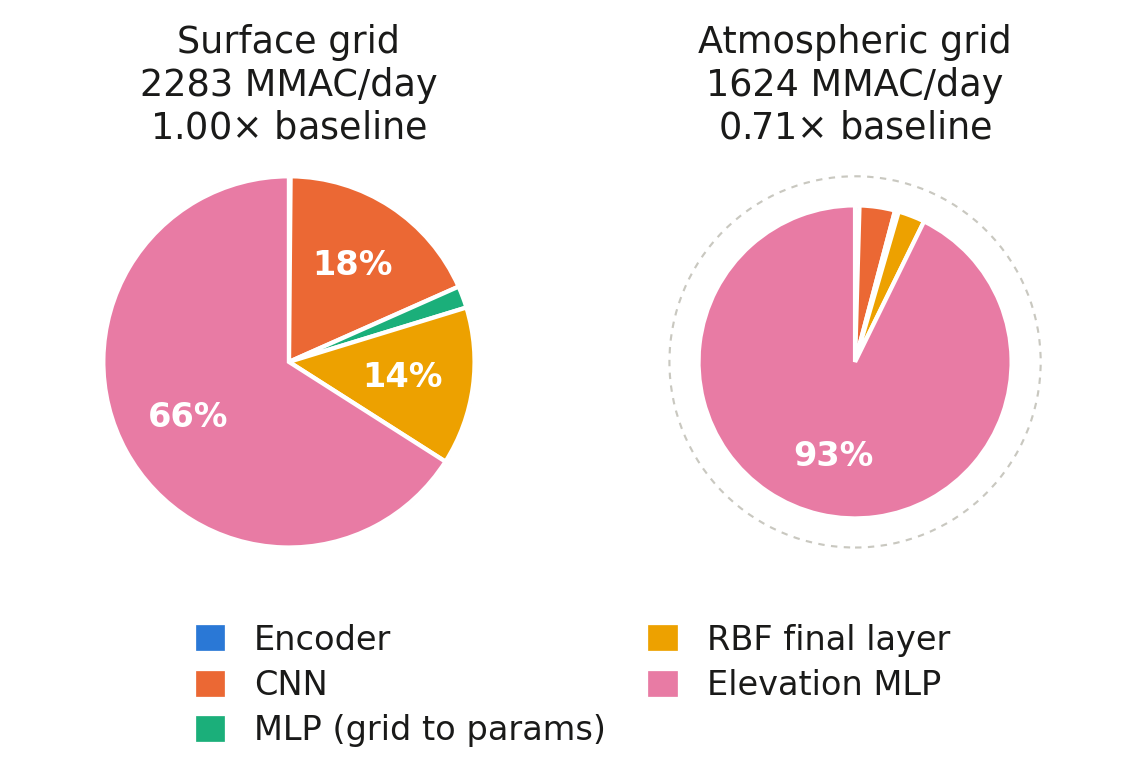
\includegraphics[width=0.75\textwidth]{images/component_cost_ops.png}
    \caption[Computational cost per component]{Computational cost per component: multiply-accumulate operations of one day, in millions, split into the architectural components.}
    \label{fig:meth-cost-ops}
\end{figure}

\begin{figure}[H]
    \centering
    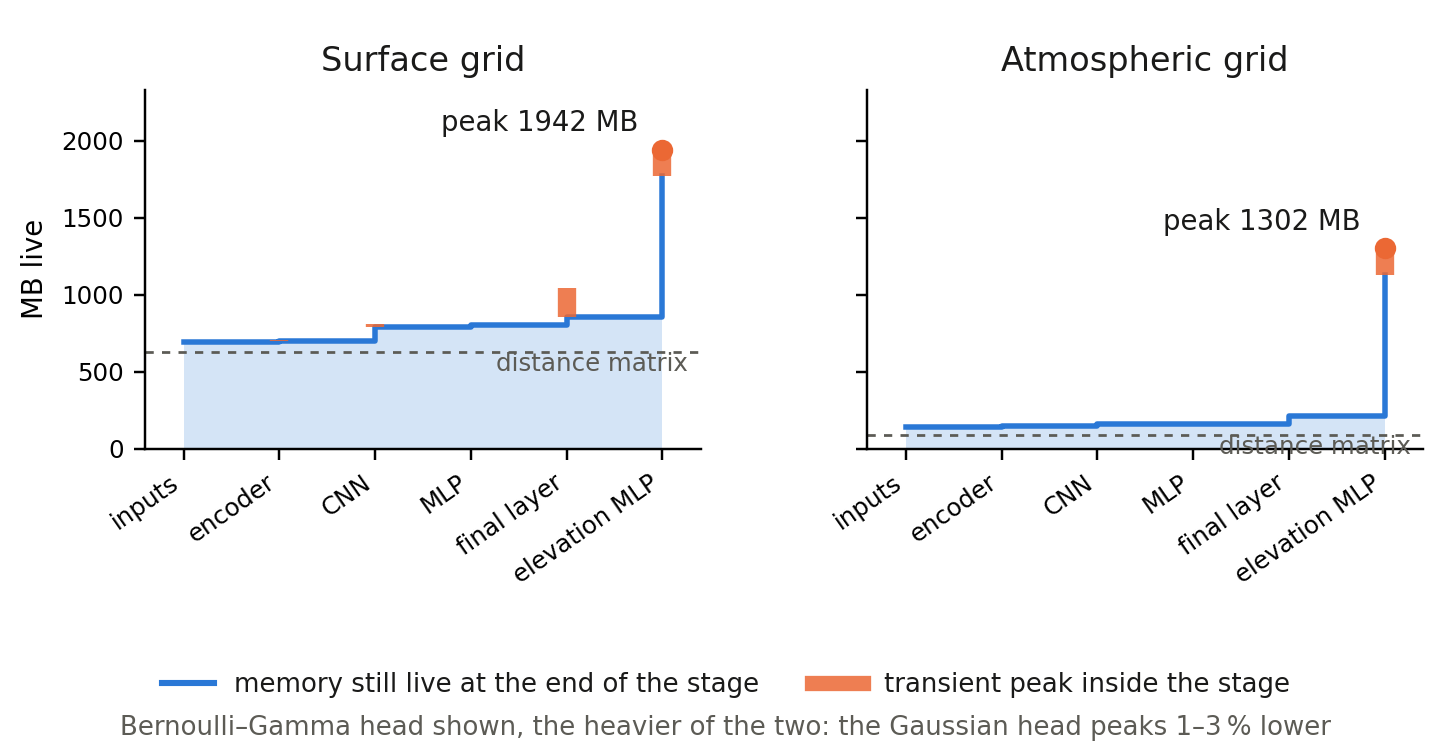
\includegraphics[width=0.86\textwidth]{images/component_cost_mem_profile.png}
    \caption[Memory through a training forward pass]{Memory estimation live at each stage of a training forward pass of the Bernoulli--Gamma configurations, the heavier of the two output heads, at the batch of eight days used in this work, with the transient inside each stage drawn above it. The peak is a moment inside a single stage, not a sum over stages.}
    \label{fig:meth-cost-mem}
\end{figure}

\FloatBarrier

Everything set out above is held fixed in what follows. The input set and the objective are the
two axes \cref{ch:single-model} varies.

% Chapter 5: Single-Model Performance  (FOCUS 1)

\chapter{Single-Model Performance}\label{ch:single-model}



This chapter evaluates the models that downscale one variable at a time. Every result is reported under the two regimes of \sref{subsec:meth-cv}: the CV holdout, where each day of 2020--2023 is predicted by the holdout fold, as well as the unseen year 2024, predicted by the five-fold ensemble. The temperature models are reported first: seven configurations are compared under both regimes, the feature-importance study explains what separates them, and the remainder of the section investigates the selected model in depth. The results of precipitation models follow in \sref{sec:single-precipitation}.



\section{Temperature Model}\label{sec:single-temperature}



\subsection{Model Variants}\label{subsec:single-tmax-variants}



\tref{tab:single-tmax-variants} lists the seven training runs behind all temperature results, with the model names used in every figure and table that follows.



\begin{table}[htbp]

\centering

\caption[The seven temperature runs]{The seven temperature runs. All share the architecture of \sref{sec:meth-architecture} and the setup of \tref{tab:meth-training-setup}; the two \texttt{-clip60} retrains (\texttt{atm-clip60}, \texttt{atm+wind-clip60}) with double the epoch budget and patience and add a gradient clip. Channel counts include the scaffold.}

\label{tab:single-tmax-variants}

\footnotesize

\begin{tabular}{|p{2.9cm}|p{6.4cm}|p{1.2cm}|p{1.2cm}|}

\hline

\textbf{Model name} & \textbf{Context input} & \textbf{Chan.} & \textbf{Epochs} \\

\hline

\texttt{sfc} & ERA5-Land daily-maximum $2\,\mathrm{m}$ temperature, plus the full scaffold & 6 & 30 \\

\hline

\texttt{sfc-nogeo} & as \texttt{sfc}, without the coarse-elevation channel & 5 & 30 \\

\hline

\texttt{atm} & ERA5 pressure-level $z$, $t$, $q$ on six levels at five sampling hours, plus scaffold & 95 & 30 \\

\hline

\texttt{atm+wind} & as \texttt{atm}, with the wind components $u$ and $v$ added & 155 & 30 \\

\hline

\texttt{atm+sfcanchors} & as \texttt{atm}, with ERA5 single-level $2\,\mathrm{m}$ temperature and total precipitation at the five hours appended & 105 & 30 \\

\hline

\texttt{atm-clip60} & as \texttt{atm}; $60$ epochs, patience $20$, gradient clip & 95 & 60 \\

\hline

\texttt{atm+wind-clip60} & as \texttt{atm+wind}; same extended budget & 155 & 60 \\

\hline

\end{tabular}

\end{table}



\subsection{Accuracy, Skill and Generalisation}\label{subsec:single-tmax-headline}



Skill is the CRPSS of \eref{eq:crpss} against the bilinear ERA5-Land reference, which is identical for every model; \tref{tab:single-tmax-headline} lists all individual numerical values for all runs. Every configuration beats the ERA5-Land reference by a wide margin: MAE falls by $1.0$ to $1.5\,^{\circ}\mathrm{C}$ and CRPS by $1.4$ to $1.8\,^{\circ}\mathrm{C}$, the atmospheric models performing better than the  surface models.

\begin{table}[H]
\centering
\caption[Temperature metrics, CV holdout vs 2024 holdout]{Headline metrics of the seven temperature runs of \sref{sec:single-temperature} under the CV holdout (2020--2023) and the 2024 holdout. All values in $^{\circ}\mathrm{C}$ except skill. Every column is comparable across the seven models: MAE, RMSE and CRPS are measured against the fixed MeteoSwiss truth, and skill, the only baseline-relative column,  is scored against ERA5-Land. Green shades the best and red the worst model in each column. The last row is the shared bilinear ERA5-Land reference: it is deterministic, so its CRPS equals its MAE and its skill is zero by definition.}
\label{tab:single-tmax-headline}
\footnotesize
\begin{tabular}{|p{3cm}|p{0.85cm}|p{0.85cm}|p{0.85cm}|p{0.85cm}|p{0.85cm}|p{0.85cm}|p{0.85cm}|p{0.85cm}|}
\hline
& \multicolumn{2}{c|}{\textbf{MAE}} & \multicolumn{2}{c|}{\textbf{RMSE}} & \multicolumn{2}{c|}{\textbf{CRPS}} & \multicolumn{2}{c|}{\textbf{Skill}} \\
\hline
\textbf{Model} & CV & 2024 & CV & 2024 & CV & 2024 & CV & 2024 \\
\hline
\texttt{atm} & 1.24 & 1.21 & 1.65 & 1.66 & 0.92 & 0.91 & 0.641 & 0.642 \\
\hline
\texttt{atm-clip60} & 1.09 & 1.05 & 1.46 & 1.42 & 0.79 & 0.76 & 0.693 & 0.702 \\
\hline
\texttt{atm+wind} & 1.31 & 1.25 & 1.73 & 1.71 & 0.96 & 0.94 & 0.625 & 0.632 \\
\hline
\rowcolor{green!12}\texttt{atm+wind-clip60} & 1.05 & 1.03 & 1.41 & 1.39 & 0.76 & 0.74 & 0.702 & 0.708 \\
\hline
\texttt{atm+sfcanchors} & 1.20 & 1.17 & 1.61 & 1.62 & 0.90 & 0.89 & 0.650 & 0.650 \\
\hline
\texttt{sfc} & 1.42 & 1.47 & 1.87 & 1.97 & 1.03 & 1.08 & 0.597 & 0.576 \\
\hline
\rowcolor{red!12}\texttt{sfc-nogeo} & 1.45 & 1.49 & 1.90 & 1.98 & 1.06 & 1.09 & 0.588 & 0.571 \\
\hline
bilinear ERA5-Land & 2.56 & 2.54 & 3.36 & 3.35 & 2.56 & 2.54 & 0 & 0 \\
\hline
\end{tabular}
\end{table}




Generalisation is strong: the best models achieve a CRPS as low as $0.74\,^{\circ}\mathrm{C}$ on the unseen year. The atmospheric models outperform the surface models on every metric (\fref{fig:single-tmax-slope}), and the gap holds on the year no fold saw. Furthermore they have potential for further improvement with an extended training budget, as evidenced by the performance of the \texttt{atm-clip60} and \texttt{atm+wind-clip60} models. The wind channels need the longer budget before they pay off: at $30$ epochs \texttt{atm+wind} ($155$ channels) is worse than \texttt{atm} ($95$), $1.31$ against $1.24\,^{\circ}\mathrm{C}$ CV MAE, while under the extended budget \texttt{atm+wind-clip60} becomes the best model of the comparison, ahead of \texttt{atm-clip60} at $1.05$ against $1.09$. The training curves show why, and show that the extended run was still improving when it ended (\sref{sec:app-tmax-metrics}). All models with atmospheric input show better generalisation than those limited to surface input.

Including surface anchors improves the performance of the atmospheric model, however the gain is small.



\begin{figure}[H]

\centering

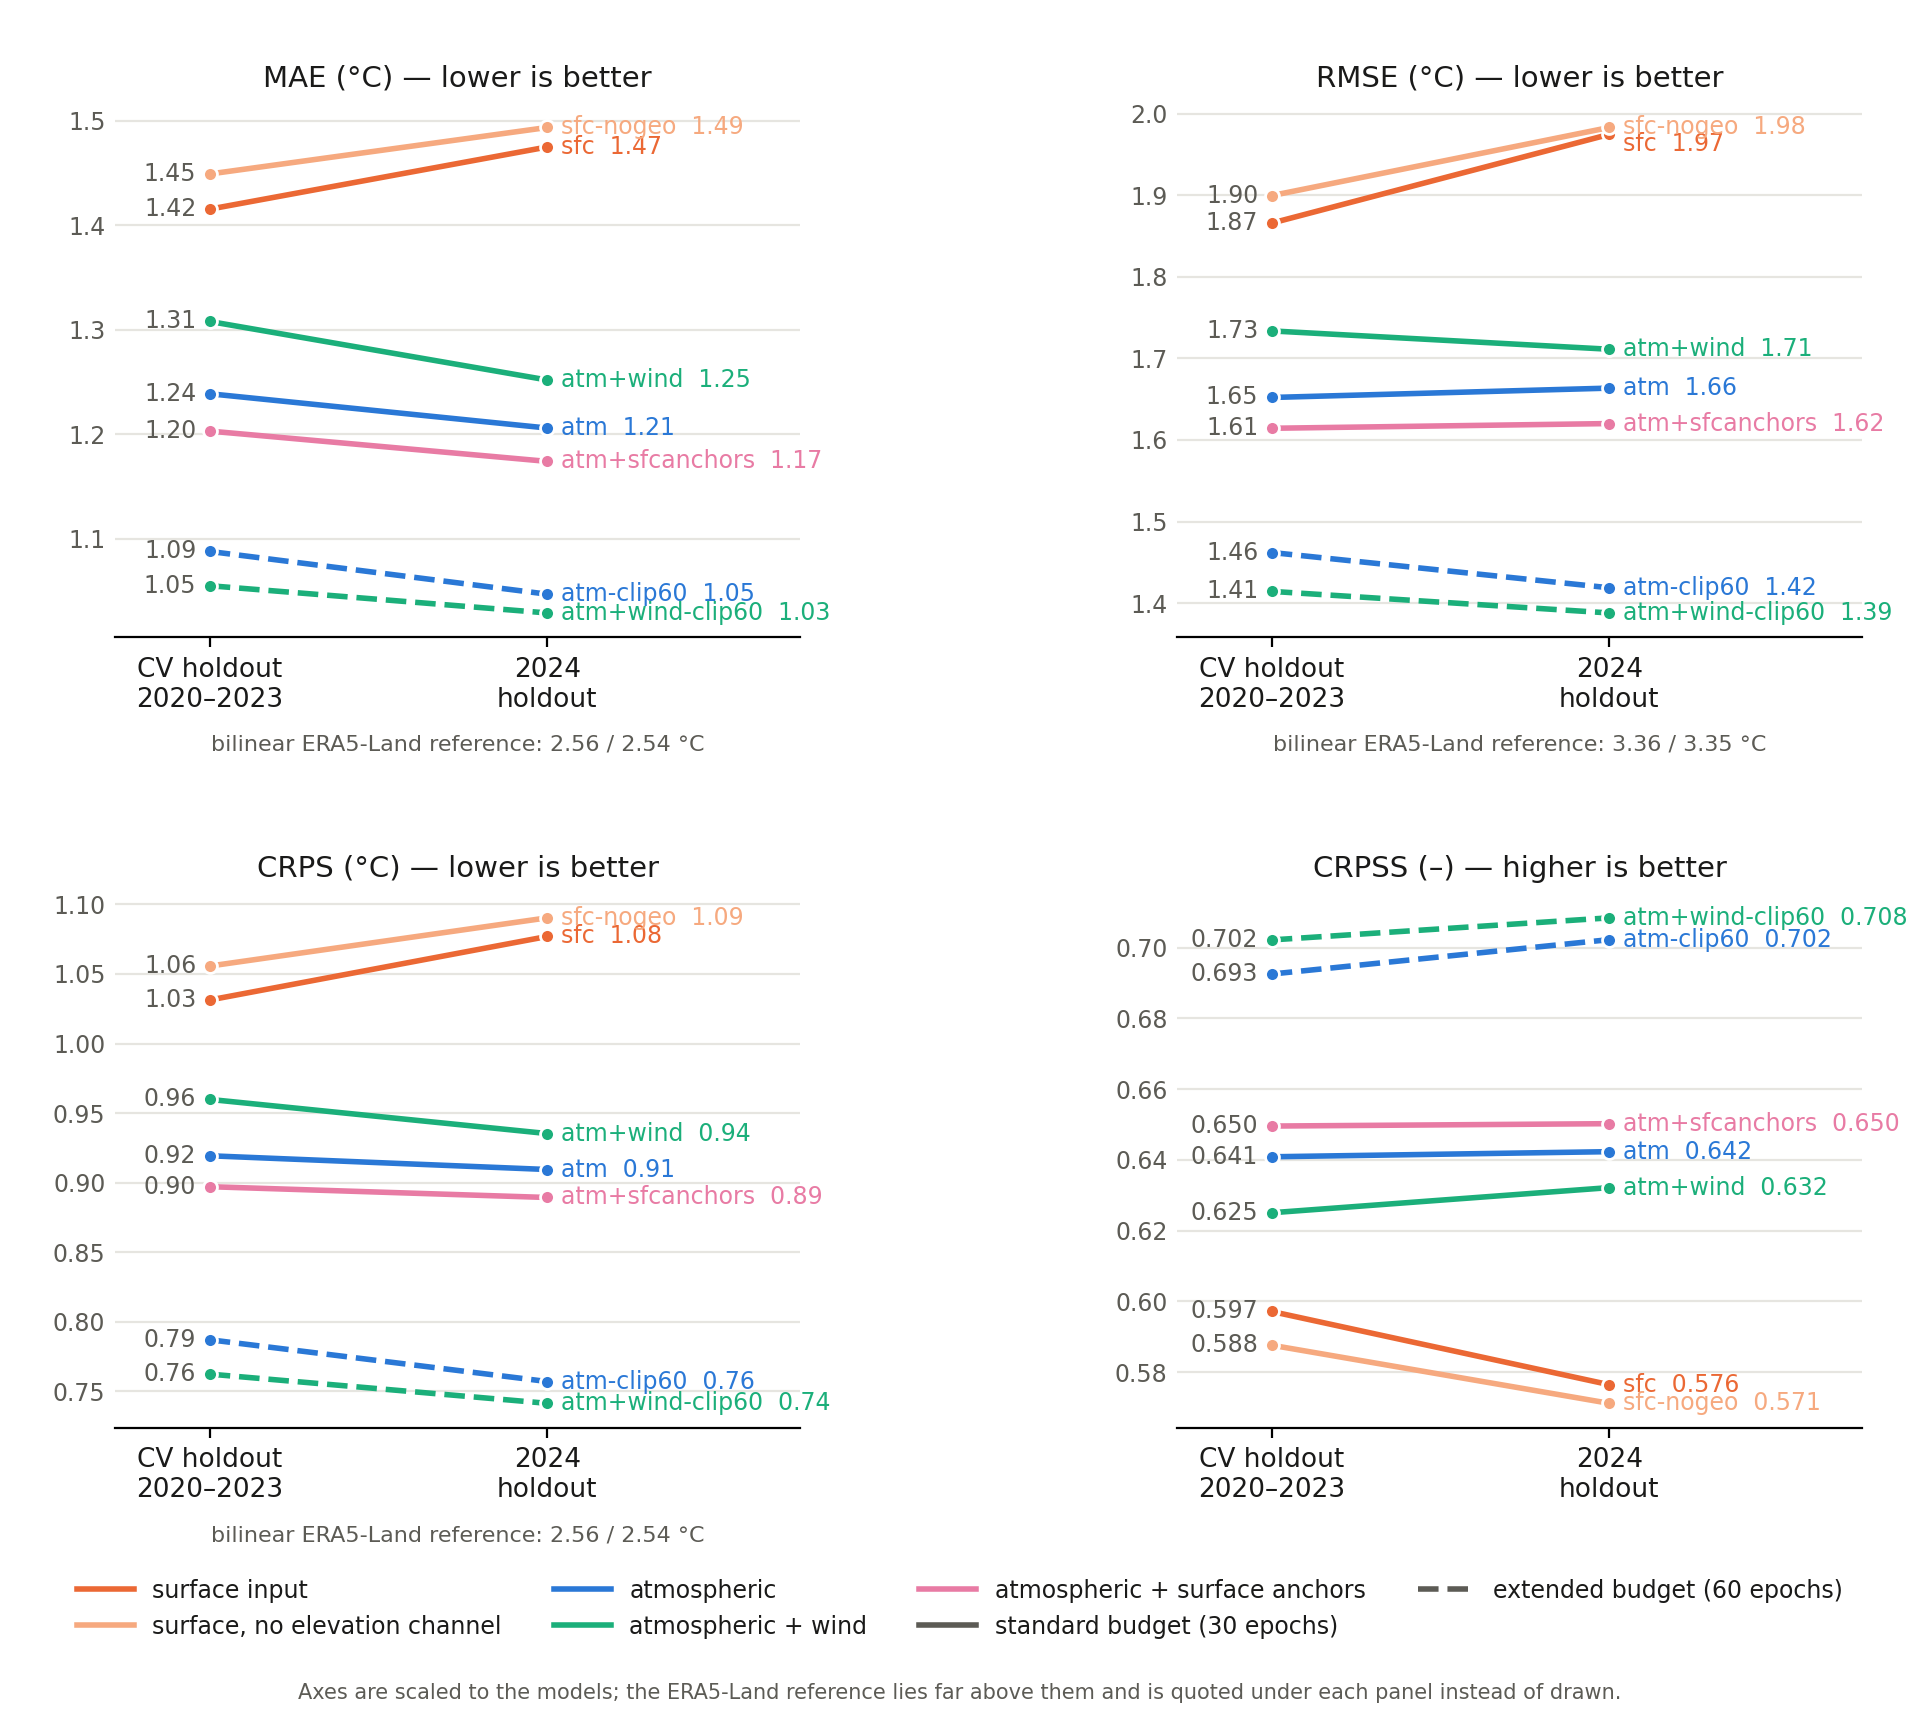
\includegraphics[width=\textwidth]{images/tmax_regime_slope.png}

\caption[Headline metrics from the CV span to 2024]{The four headline metrics of the seven temperature models. Colour encodes the input family, dashed lines the extended-budget retrains. It is clearly visible that the atmospheric input models perform well and generalise well. The surface models lag behind and the generalisation is worse than the CV.}

\label{fig:single-tmax-slope}

\end{figure}







\subsection{Feature Importance}\label{subsec:single-tmax-fi}

For the feature-importance study on temperature we first have a look at the grouped importance for the two input families atmospheric input and surface input. As an additional reference we consider the atmospheric input with the surface anchors. While the surface anchors include the diurnal cycle they are the closest match to the surface input while still being part of the atmospheric input family. All results are evaluated on the 2024 holdout year.





\begin{figure}[H]

\centering

\subfloat[\texttt{sfc}]{%

  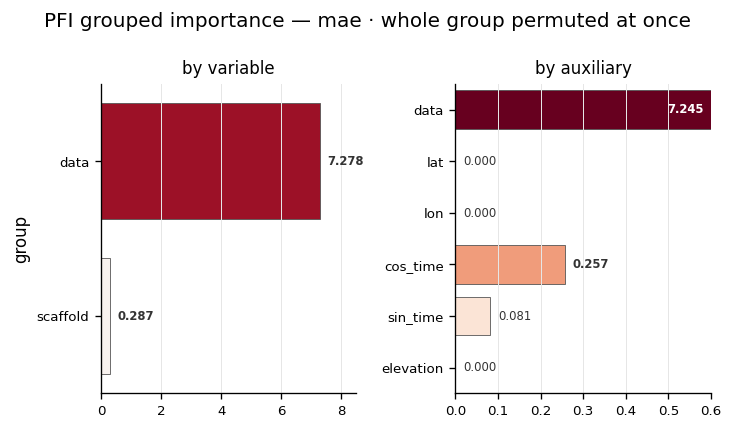
\includegraphics[height=0.285\textwidth]{images/results/tmax__pfi_groups_mae__feature_importance_2024__baseline.png}}\\[2ex]

\subfloat[\texttt{atm}]{%

  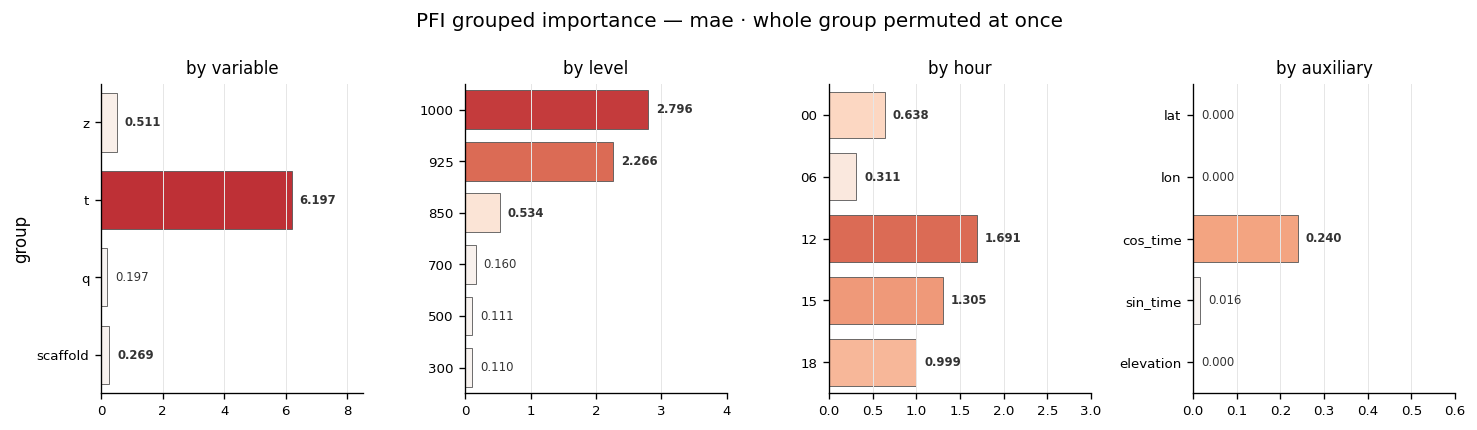
\includegraphics[height=0.285\textwidth]{images/results/tmax__pfi_groups_mae__feature_importance_2024__clean_solo.png}}\\[2ex]

\subfloat[\texttt{atm+sfcanchors}]{%

  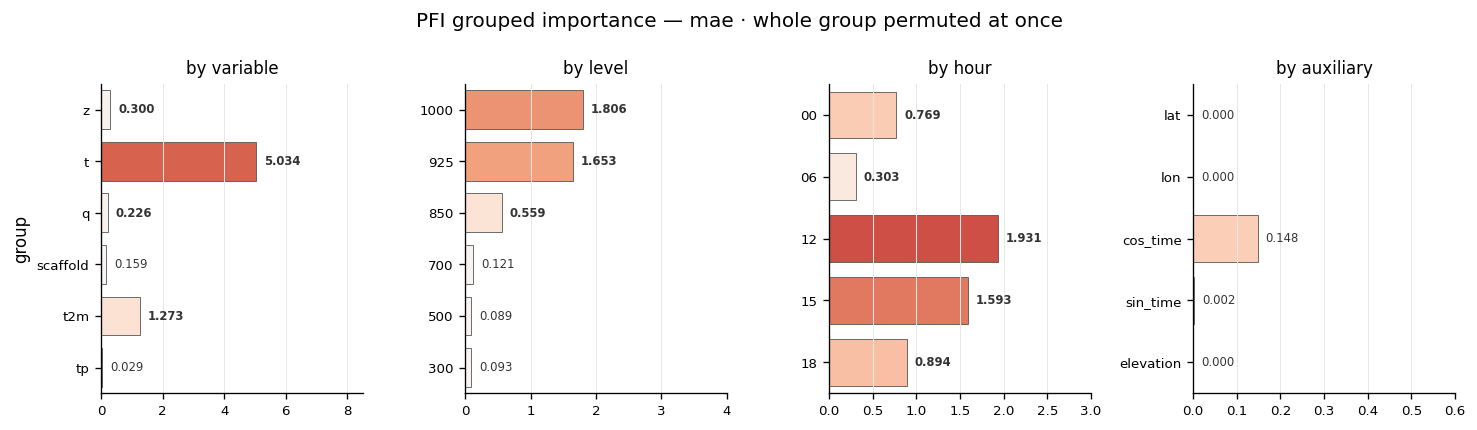
\includegraphics[height=0.285\textwidth]{images/results/tmax__pfi_groups_mae__feature_importance_2024__sfc_anchors.png}}

\caption[Grouped permutation importance across the three input families]{Grouped permutation importance (\sref{subsec:meth-fi-groups}) for the three $30$-epoch input families: the MAE degradation in $^{\circ}\mathrm{C}$ when a whole group is permuted at once. All three models are dominated by close to surface temperature; for the surface model, the seasonal encoding is the only other group with visible impact. The atmospheric input models also show a significant importance of the diurnal cycle information. Even though low altitude pressure levels  in the second half of the day dominate the importance, the higher levels and even night time snapshots still contribute in a non negligible way.}

\label{fig:single-tmax-fi-groups}

\end{figure}
 \fref{fig:single-tmax-fi-groups} presents a good overview to compare the reliance of the different input families. The surface model (a) has only one data source, its data channel carries $7.3\,^{\circ}\mathrm{C}$ of importance, with the seasonal encoding ($0.26$ for its stronger channel) the only other visible input with impact. The remaining scaffold channels score exactly zero, this is by design as a time-invariant channel is unchanged by a permutation along the day axis (\sref{subsec:app-fi-limits}). The atmospheric model (b) spreads a similar importance across its temperature group ($6.2\,^{\circ}\mathrm{C}$), concentrated at $1000$ and $925\,\mathrm{hPa}$ and in the midday and afternoon hours, while geopotential and humidity contribute little but not nothing. With the anchors added (c) the pattern persists, but the $2\,\mathrm{m}$ anchor takes a substantial share ($1.3\,^{\circ}\mathrm{C}$, against $5.0$ for the temperature group) while the precipitation anchor is ignored, and the seasonal encoding falls to its smallest value of the three ($0.15$). The same grouped view for the four remaining configurations is in \sref{sec:app-fi}. The surface anchors are therefore not a substitute for the atmospheric input, but they do provide a small additional signal that the model can use.







Temperature is a relatively easy variable to downscale, so it is not surprising that the surface input model is able to achieve a good performance with only one temperature channel. What remains to be observed here is that the atmospheric input model while missing any meteorological surface input is able to achieve better performance than the surface input model. Therefore we can conclude that the atmospheric input contains more information than the surface input and that the model is able to extract and learn this information. Adding surface anchors gains a slight advantage over the atmospheric input model, but the feature importance study shows that the model still relies on the atmospheric input and does not overwrite the learned information with the surface anchors. 



\subsection{The Downscaled Field}\label{subsec:single-tmax-field}

Before turning to the error statistics we look at the spatial patterns of the modelled fields. \fref{fig:single-tmax-spatial} shows snapshots of the downscaled field. The coarse input resolves the domain into a handful of smooth patches; along the section we have significant alpine topography and cross the Main alpine divide. The reference model does not resolve the terrain details; both downscaling models return the valley-and-ridge swing of the ground-truth reference.

\begin{figure}[htbp]

\centering

\subfloat[A typical day: 25 January 2024, the median-error day with the widest observed range]{%

  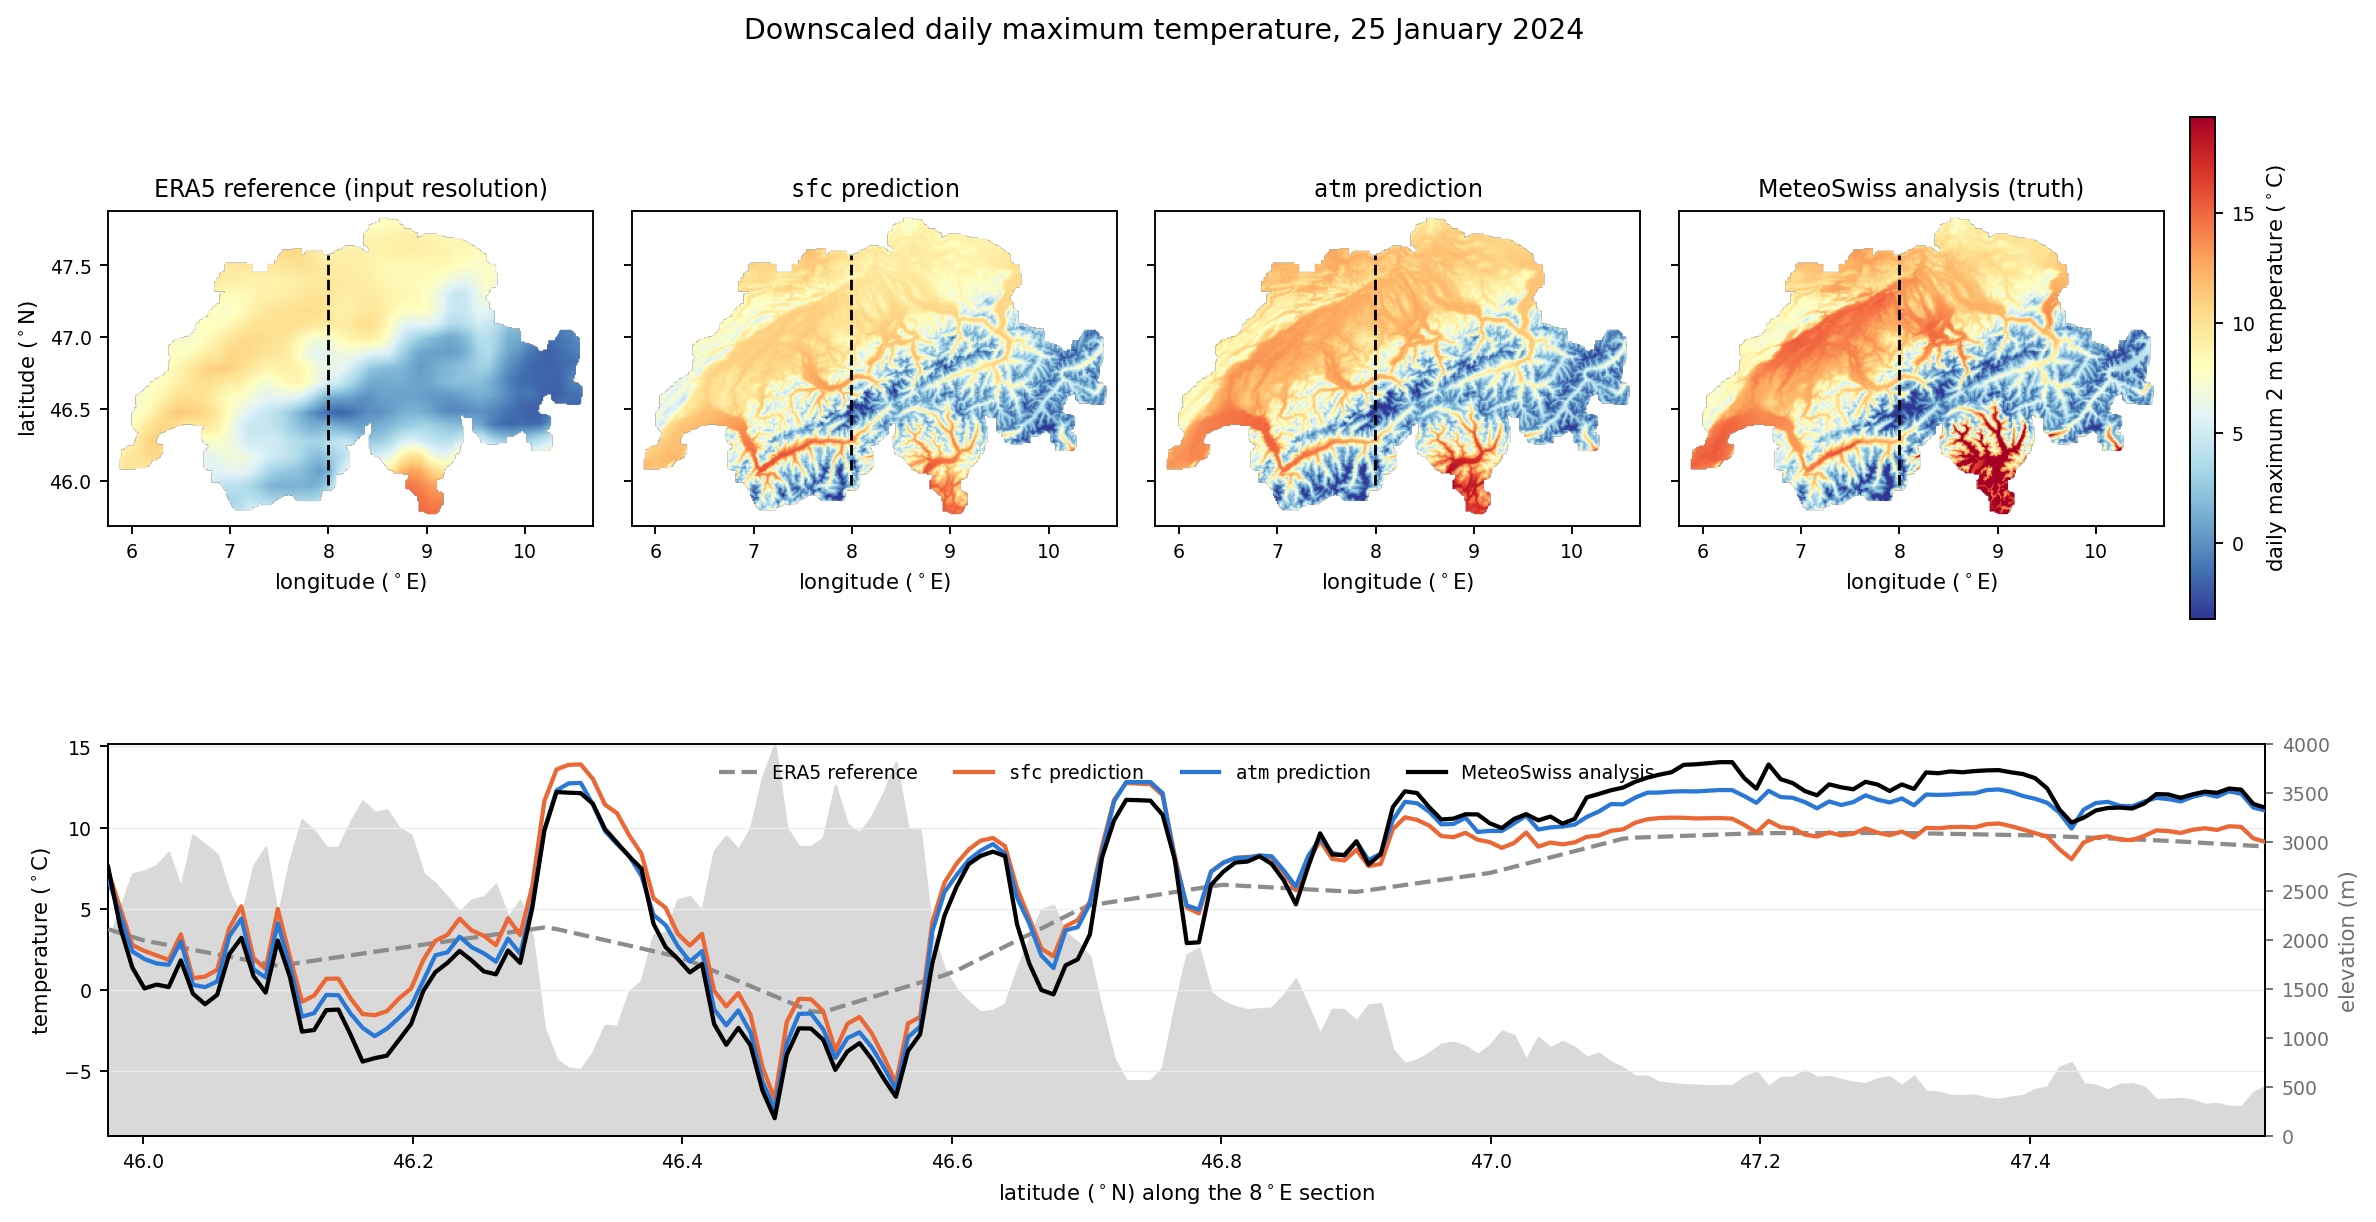
\includegraphics[width=0.74\textwidth]{images/tmax_spatial_section.png}}\\[1ex]

\subfloat[The extreme warm day: 30 July 2024, the highest observed domain-mean maximum]{%

  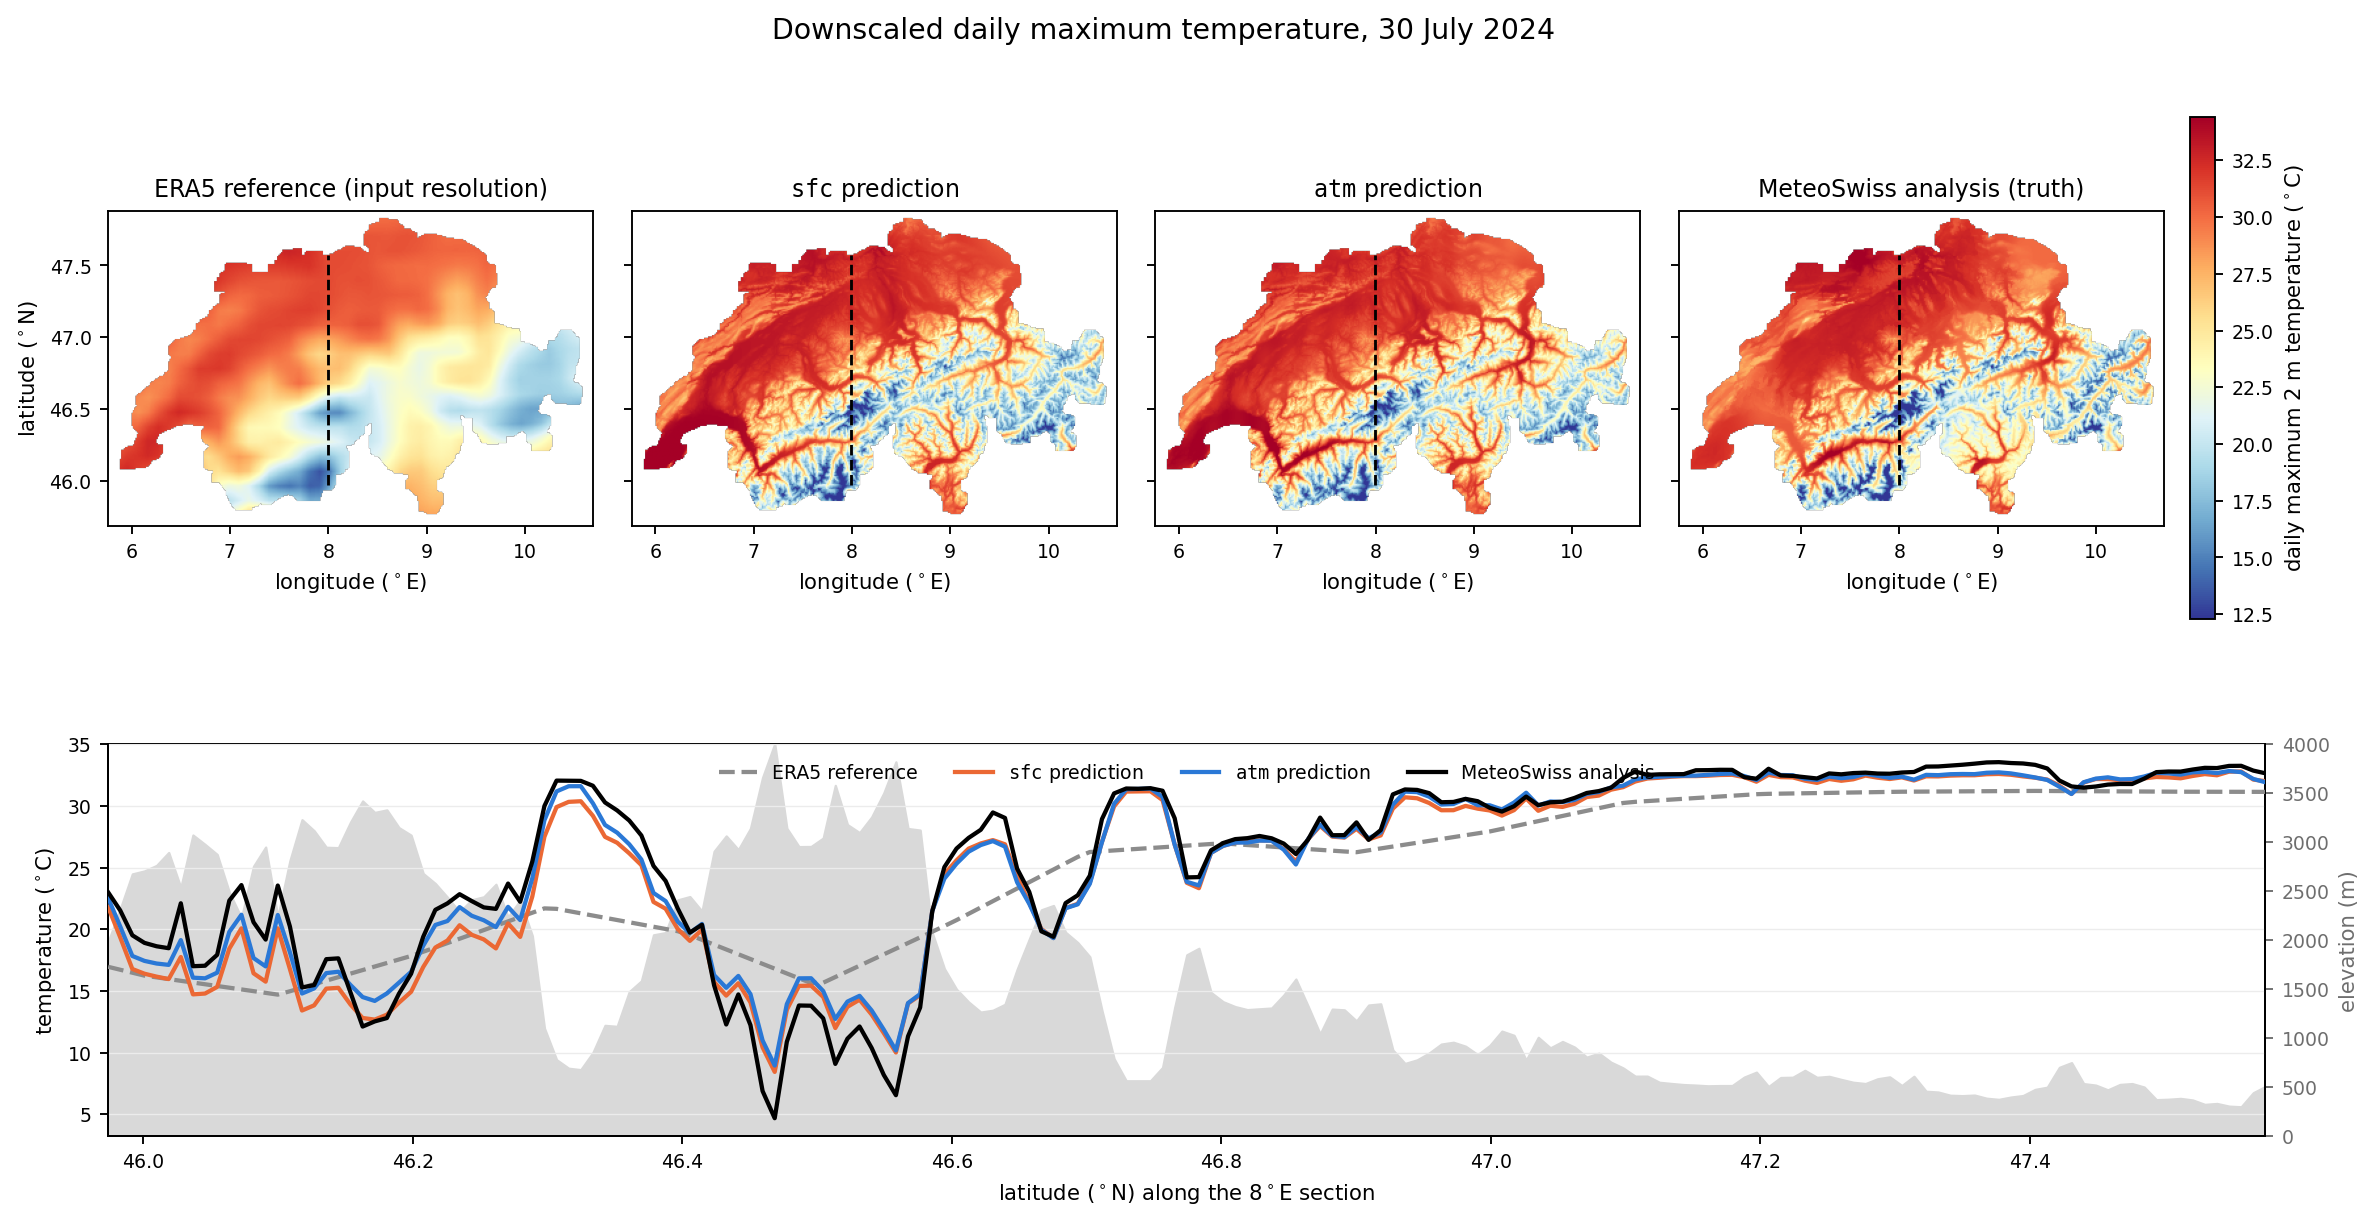
\includegraphics[width=0.74\textwidth]{images/tmax_spatial_section_warm.png}}

\caption[Downscaled field and temperature profile along a terrain section]{Downscaled field and temperature profile along a terrain section. On the top left of both figures we have the coarse-grid ERA5-Land surface temperature reference. On the top right the ground-truth MeteoSwiss Tmax field. In between the predictions for the surface and the atmospheric models. Below we have a south-to-north cross-section over the terrain and its temperature profile. These snapshots of two difficult days of the year show how well the temperature models are able to reconstruct the fine resolution of the terrain and the temperature field. The atmospheric model is able to follow the terrain profile more closely than the surface model. On the cold-weather day the surface model shows significant deterioration over the flat terrain of the Plateau while the atmospheric model is able to follow the ground truth. On the warm day both models are able to follow the terrain profile and the ground truth.}

\label{fig:single-tmax-spatial}

\end{figure}



Upon studying these two figures we notice a distinct difference in the reference forecast. Over the relief the reference is off by many degrees on both days, but that error is systematic, tied to the smoothed orography, and both models correct it in winter and summer alike. The offset we observe in winter over the Plateau is a different failure: there the target temperature runs about three degrees warmer than anything the reference field suggests. This offset, occurring only on the cold day and on the plateau originates in the daily conditions rather than in the missing orography. \texttt{sfc}, whose only meteorological signal is the surface temperature field cannot detect the systematic error and inherits the bias from the reference; \texttt{atm} can pick it up from the atmospheric context and follows the trends of the target.  On the warm day no such departure occurs and the two models are nearly equivalent. The surface input therefore suffices while the fine-scale truth follows the coarse field in a predictable way, and fails where the two decouple. Two chosen days are only illustrations, but \fref{fig:single-tmax-decoupling} extends these observations to the whole domain. It splits the observations into two elevation bands, below $600\,\mathrm{m}$ and above $2000\,\mathrm{m}$, and plots the monthly MAE for the reference and the two $30$-epoch models. The seasonality of the error is clear: the reference error is largest in the cold months. The atmospheric model only shows a slight increase of error for the cold months, while the surface model approaches the reference error in the cold months. This observation is equally valid for the lowlands and the high Alps therefore the origin is seasonal rather than geographic. The effect is even more pronounced when observing the holdout data 2024 (thin lines), where in the cold months the surface model and the reference are nearly identical.

\FloatBarrier

\begin{figure}[H]

\centering

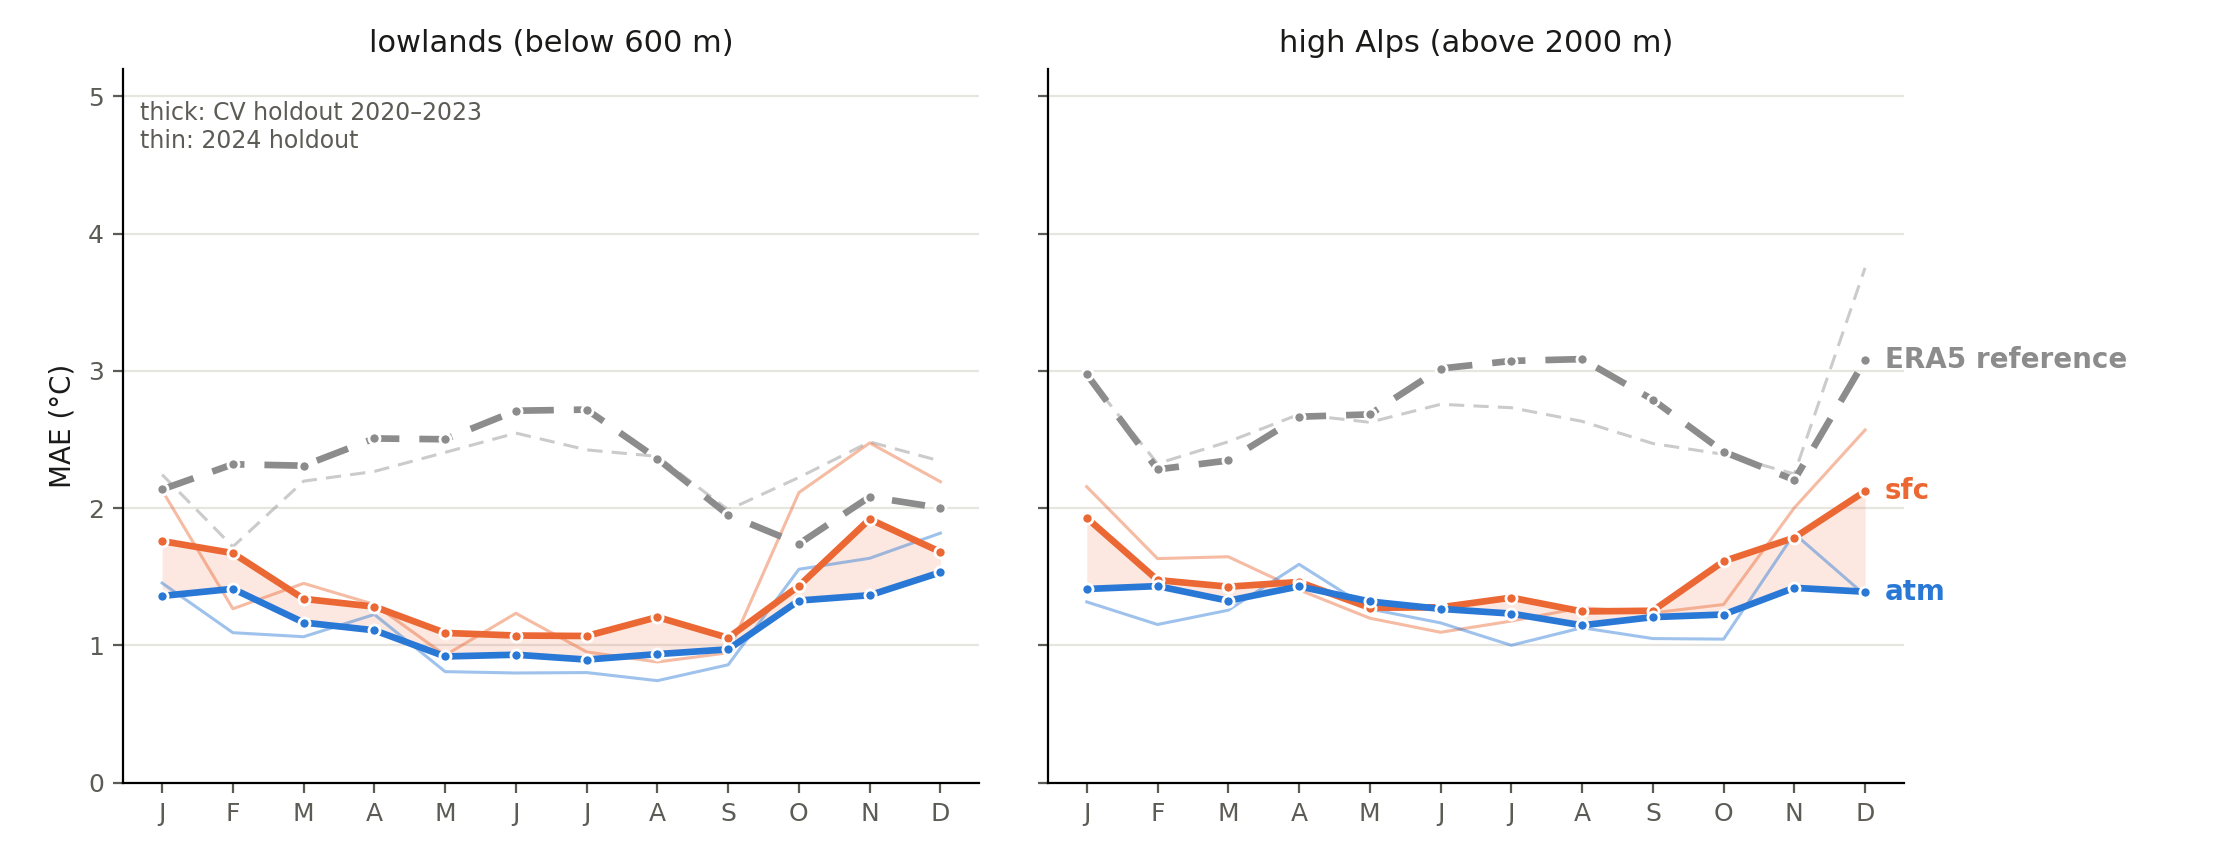
\includegraphics[width=0.9\textwidth]{images/tmax_seasonal_decoupling.png}

\caption[Seasonal decoupling of the surface input]{Seasonal decoupling of the surface input, read from the monthly MAE for the reference and the two $30$-epoch models \texttt{sfc} and \texttt{atm} over the lowlands (left, below $600\,\mathrm{m}$) and the high (right, above $2000\,\mathrm{m}$). Thick lines: the CV holdout 2020--2023, so each month is backed by four years; thin lines: the 2024 holdout. Both models stay well below the reference in every month of both bands. The systematic relief error is corrected year-round,  while the gap between \texttt{sfc} and \texttt{atm} (shaded) opens in the cold months and closes in summer, in both bands}

\label{fig:single-tmax-decoupling}

\end{figure}



\subsection{Model Selection}\label{subsec:single-tmax-geography}

\fref{fig:single-tmax-maecrpsmaps} maps both error metrics MAE and CRPS for the sfc and atm models and for the two atmospheric models with extended training. The same terrain signature appears in every panel: the overall error concentrates along the inner-Alpine valley floors and is lowest over the Plateau. The performance improvement from left to right is visible over the whole domain rather than confined to any one region. Longer training leads to significant improvements and starts, for the wind model, to reduce the error even in the valleys (green circles). CRPS and MAE agree on this spatial pattern. \fref{fig:single-tmax-windgain}, the direct comparison between the two extended-budget atmospheric models, highlights this positive impact of the wind input. So the improvement is strongest where the downscaling is hardest, along the inner-Alpine valley systems, and weakest along the Jura crest. The wind input is therefore not a general improvement, but a targeted one that helps most where it is needed. On average the wind channels buy little, a median gain of $+0.03\,^{\circ}\mathrm{C}$ per grid point with an improvement at $70\,\%$ of them, and the gain concentrates along the Rh\^one, Ticino, Grisons and Alpine Rhine valleys while the Jura crest is ceded. It is also a caution against reading permutation importance as the whole story: the $u$ and $v$ groups score near the bottom of the wind model's own importance ranking (\fref{fig:app-fi-sel-tmax}), yet carry a locally valuable signal that the global average hides.

\begin{figure}[H]

\centering

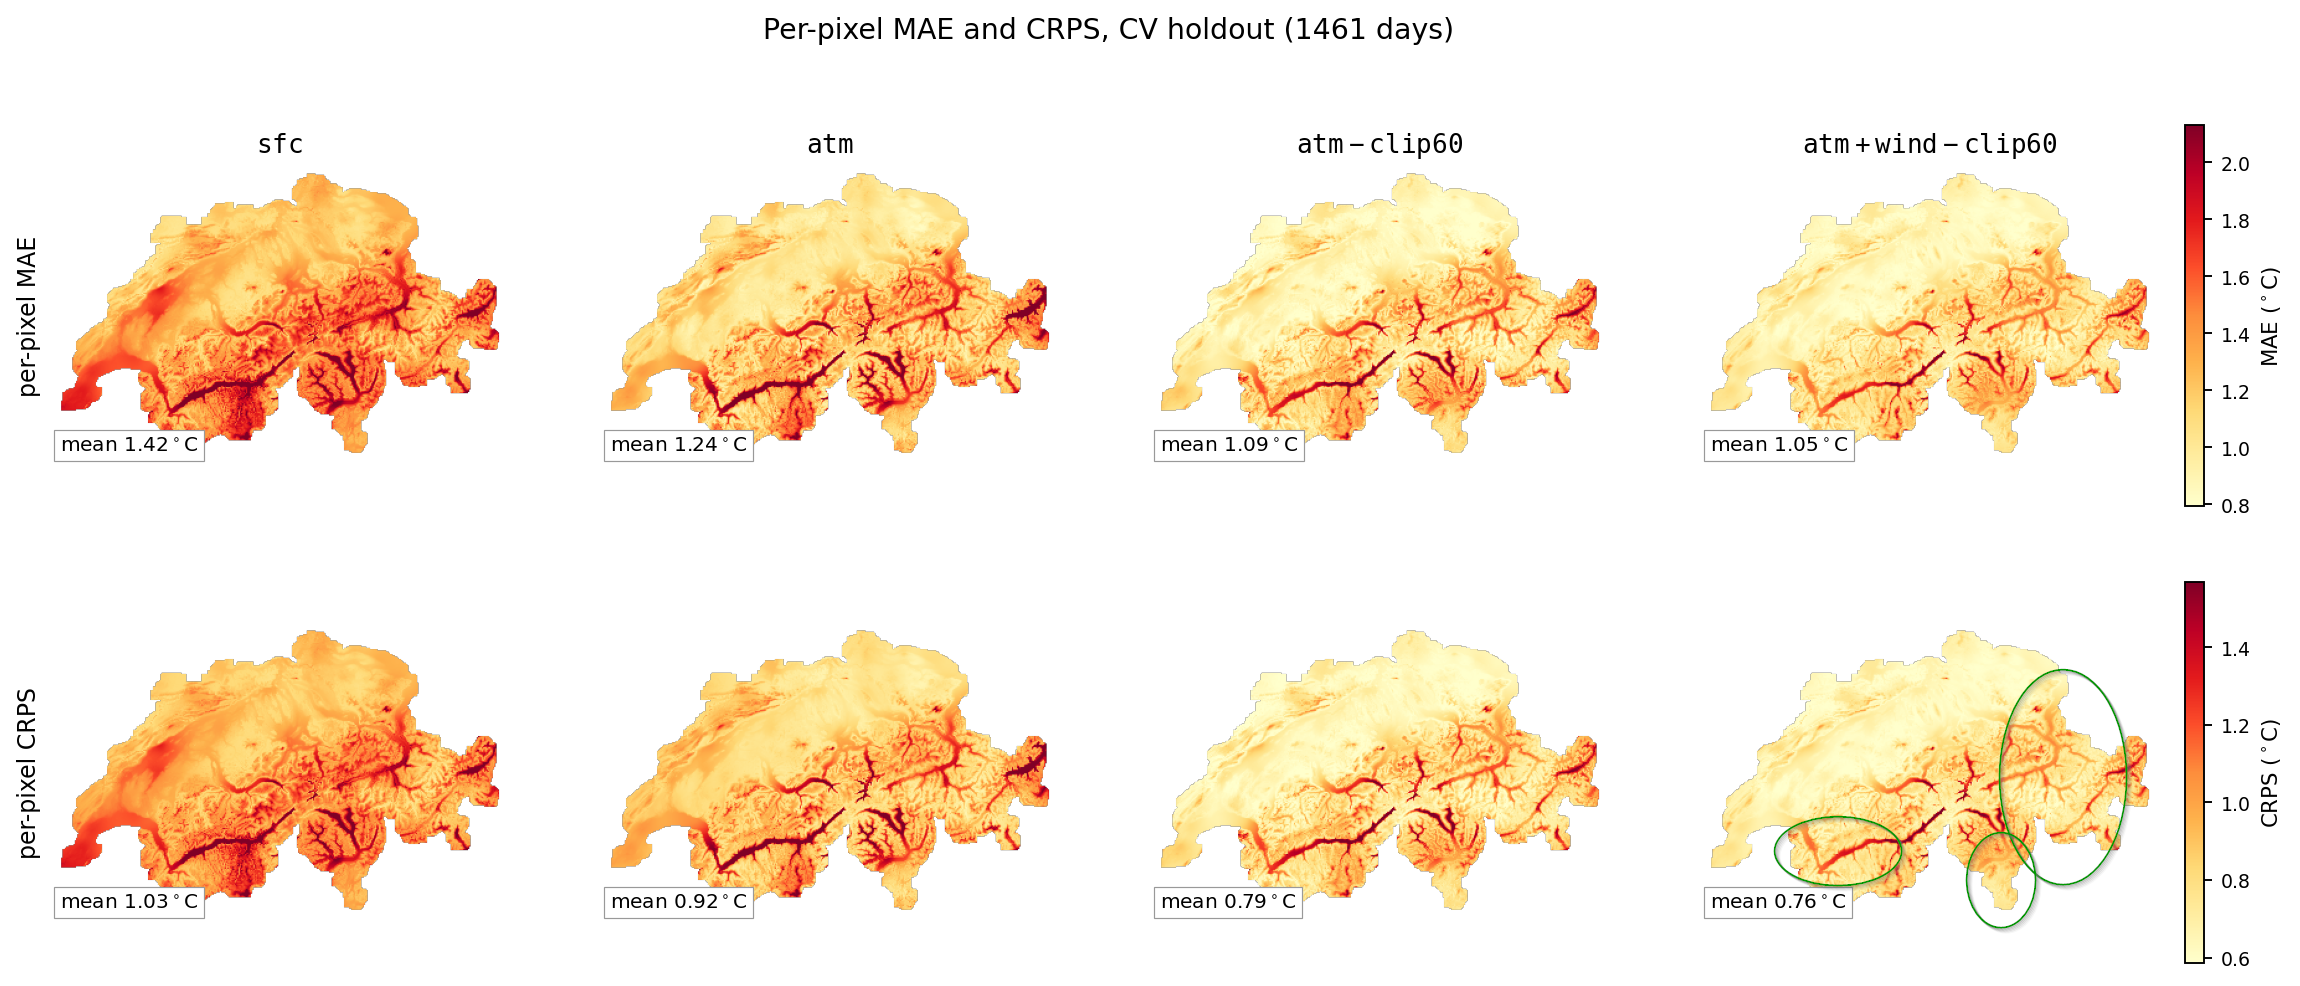
\includegraphics[width=\textwidth]{images/tmax_mae_crps_maps.png}

\caption[Per-pixel MAE and CRPS across four configurations]{Per-pixel MAE and CRPS over the CV holdout, for the two reference models (\texttt{sfc}, \texttt{atm}) and the two extended-budget atmospheric models (\texttt{atm-clip60}, \texttt{atm+wind-clip60}). Each row shares one colour scale, set to the 1st and 99th percentiles of the pooled distribution; the domain mean is given in each panel.}

\label{fig:single-tmax-maecrpsmaps}

\end{figure}







\begin{figure}[H]

\centering

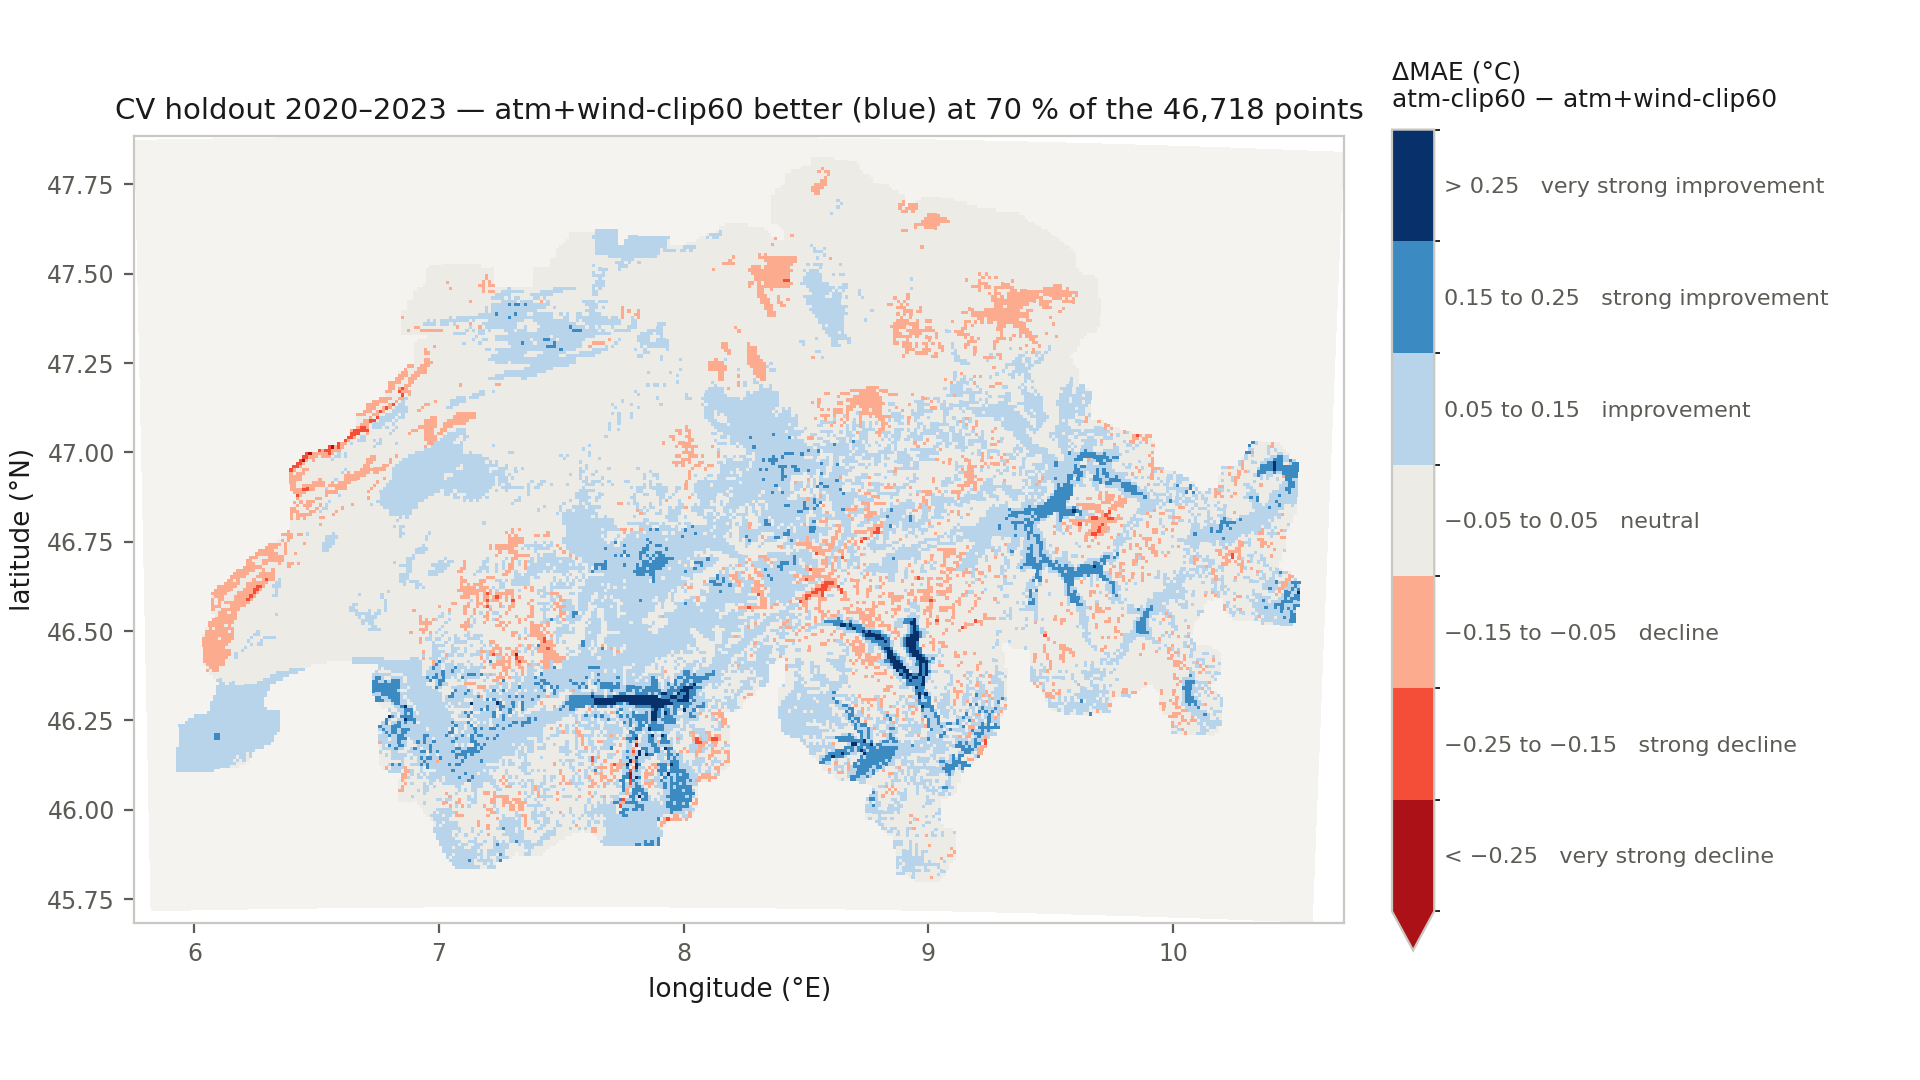
\includegraphics[width=0.9\textwidth]{images/tmax_wind_gain_map.png}

\caption[Where the wind input pays off]{Per-grid-point MAE saved by \texttt{atm+wind-clip60} over \texttt{atm-clip60} on the CV holdout. The gain concentrates along the inner-Alpine valley systems and 70\% of the points are improved. Loss is observed on isolated regions including some high altitude peaks and systematically and along the western border of switzerland.}

\label{fig:single-tmax-windgain}

\end{figure}






On this evidence we choose from here on to focus on the \texttt{atm+wind-clip60} model as the best performing model, and report the remaining results on it. The error of the selected model against terrain height and terrain position is shown in \fref{fig:single-tmax-terrain}. 



Every comparison in this subsection, and the choice itself, rests on the CV holdout, so the final selection between \texttt{atm-clip60} and \texttt{atm+wind-clip60} consumes only the training span; the unseen year entered the argument beforehand only through the aggregate generalisation check of \sref{subsec:single-tmax-headline} and the feature-importance study of \sref{subsec:single-tmax-fi}, which both are scored on 2024. The subsections that follow reverse the roles and report the selected model on 2024, as an example for the regime in which it would actually be deployed. This introduces new weather conditions the model has never seen, so the evaluation is a genuine test of how that specific choice generalises.



\subsection{Model Evaluation and Generalisation}\label{subsec:single-tmax-unseen}



\begin{figure}[H]

\centering

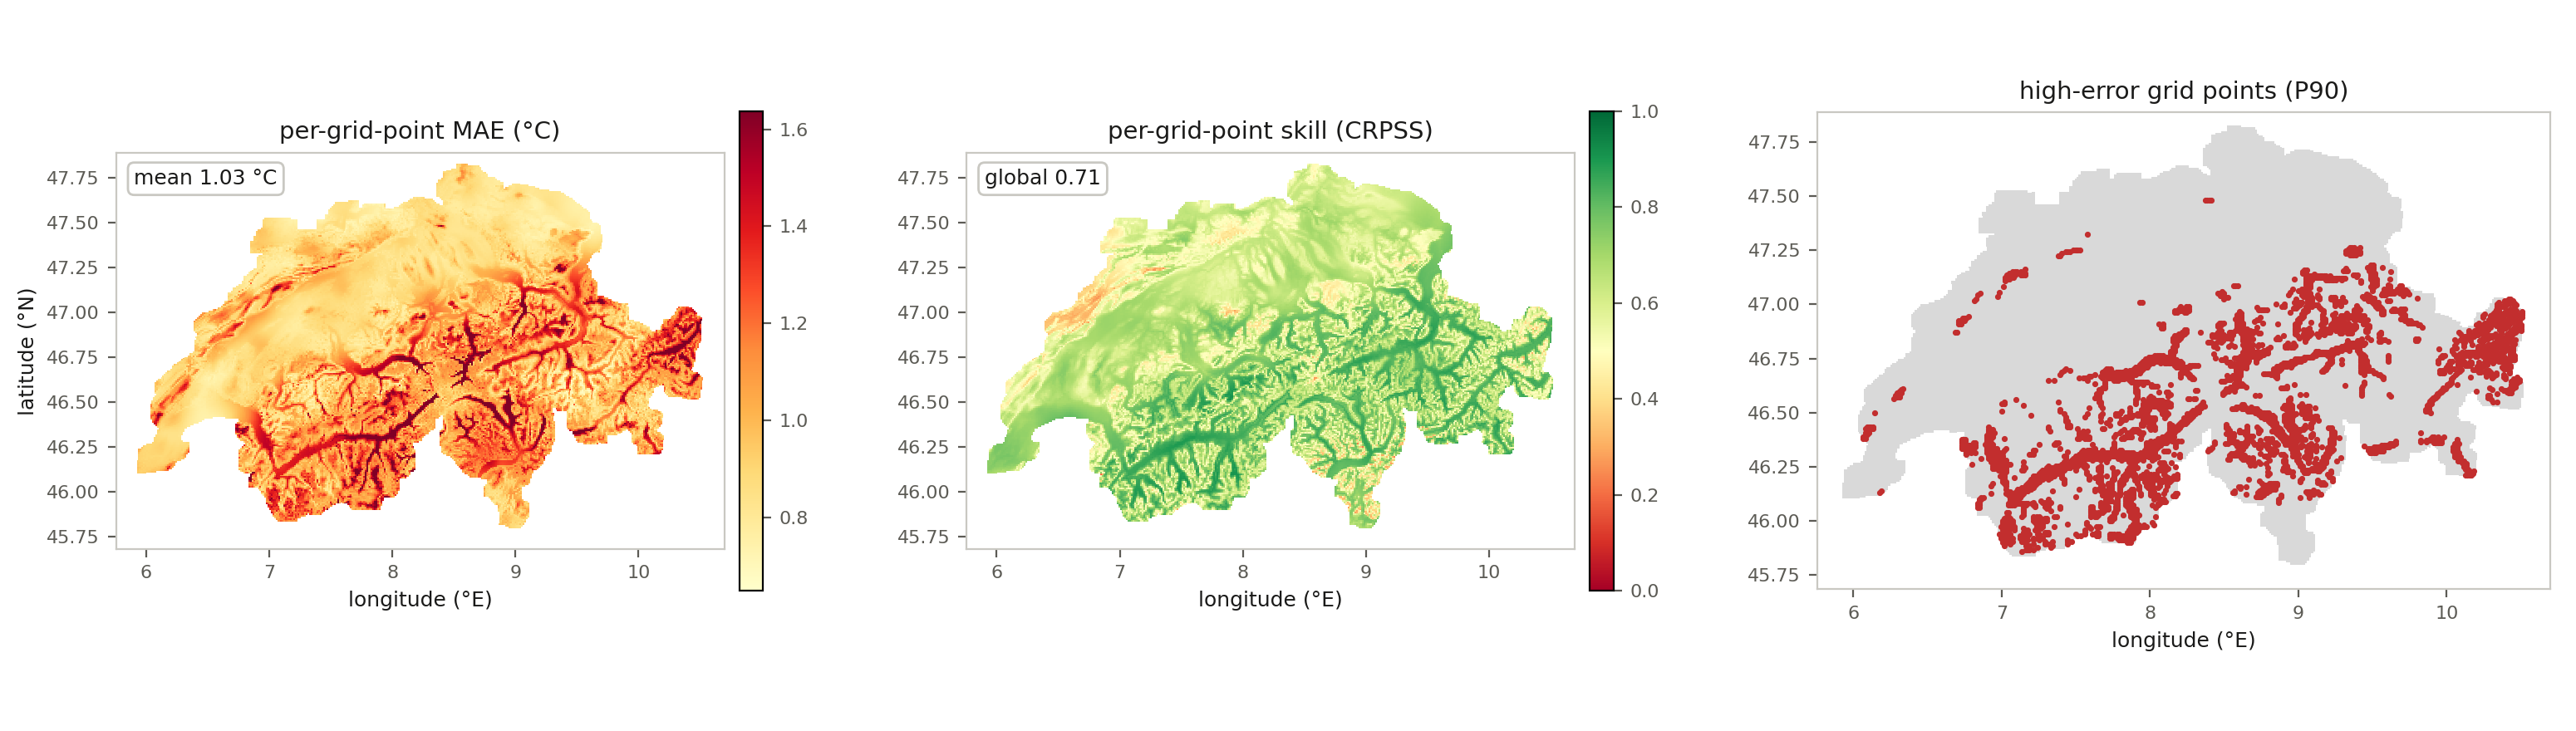
\includegraphics[width=\textwidth]{images/tmax_wind_2024_maps.png}

\caption[Where the error lives on the map]{Where the error lives on the map: \texttt{atm+wind-clip60} evaluated on the 2024 holdout. Per-grid-point MAE (left), per-grid-point skill against the bilinear ERA5-Land reference (centre), and the grid points above the 90th error percentile (right). The high-error set traces the inner-Alpine valley systems and some ridgelines, as well as the peak ridges in the Jura area. The Jura crest is the only region where the model only provides a marginal improvement over the reference.}

\label{fig:single-tmax-maemap}

\end{figure}



In the generalisation regime, the model reaches a global skill of $0.71$ against the bilinear ERA5-Land reference, with a MAE of $1.03\,^{\circ}\mathrm{C}$, slightly better than on the training span. The high MAE zones in \fref{fig:single-tmax-maemap} confirm the pattern of the CV maps: the lowlands sit at $0.7$--$0.9\,^{\circ}\mathrm{C}$ while  the inner-Alpine valley floors and ridgelines present the highest $10\,\%$ of errors. However when observing the  skill panel, it becomes clear that the model scores highest along the very valleys where its absolute error is largest. This is a direct result of the reference completely lacking accuracy in these regions. The lowest skill of the model is observed in the northwest Jura area.



When looking at the domain mean bias we can observe that the model has a tendency to overestimate temperatures. This bias grows from $+0.08\,^{\circ}\mathrm{C}$ on the CV span to $+0.23\,^{\circ}\mathrm{C}$ on 2024. \fref{fig:single-tmax-biasdrift} visualises the drift by calendar month: the 2024 curve sits above the CV curve in every month of the year, by $0.15\,^{\circ}\mathrm{C}$ on average and without seasonal concentration. The drift therefore behaves as a near-constant offset through the year.



\begin{figure}[H]

\centering

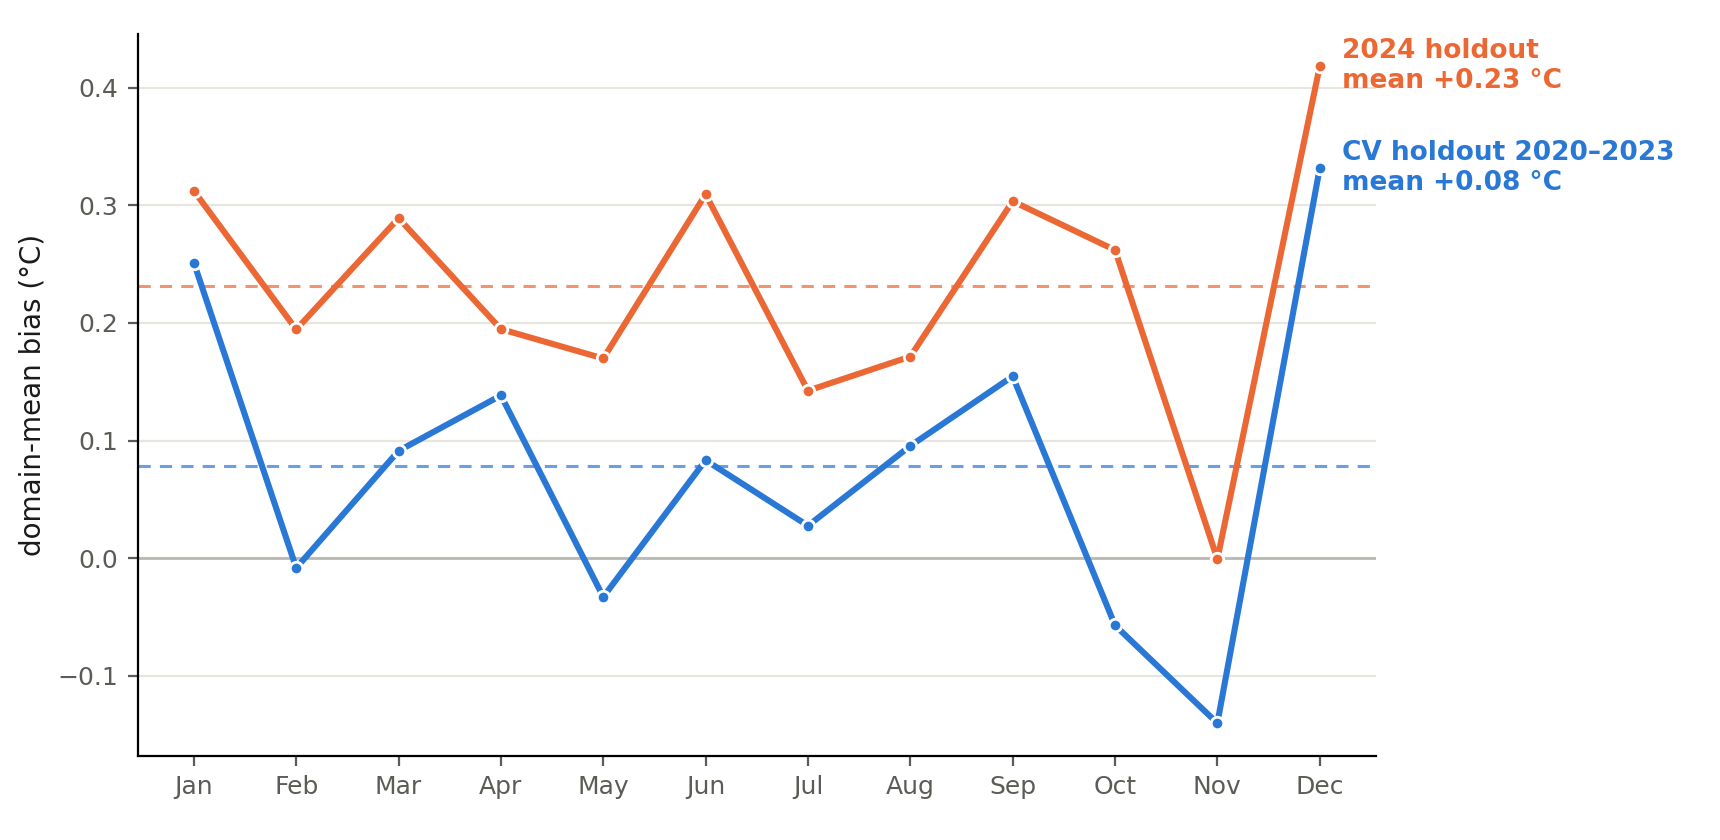
\includegraphics[width=0.9\textwidth]{images/tmax_bias_drift.png}

\caption[The warm drift on the unseen year]{The warm drift on the unseen year, read from the monthly domain-mean bias of \texttt{atm+wind-clip60} on the CV holdout and on 2024. Dashed lines mark the regime means. This shows that the warm drift on 2024 is nearly constant through the year.}

\label{fig:single-tmax-biasdrift}

\end{figure}



\subsection{Calibration and Distribution}\label{subsec:single-tmax-calibration}



\begin{figure}[H]

\centering

\subfloat[CV holdout 2020--2023, single-fold $\sigma$]{%

  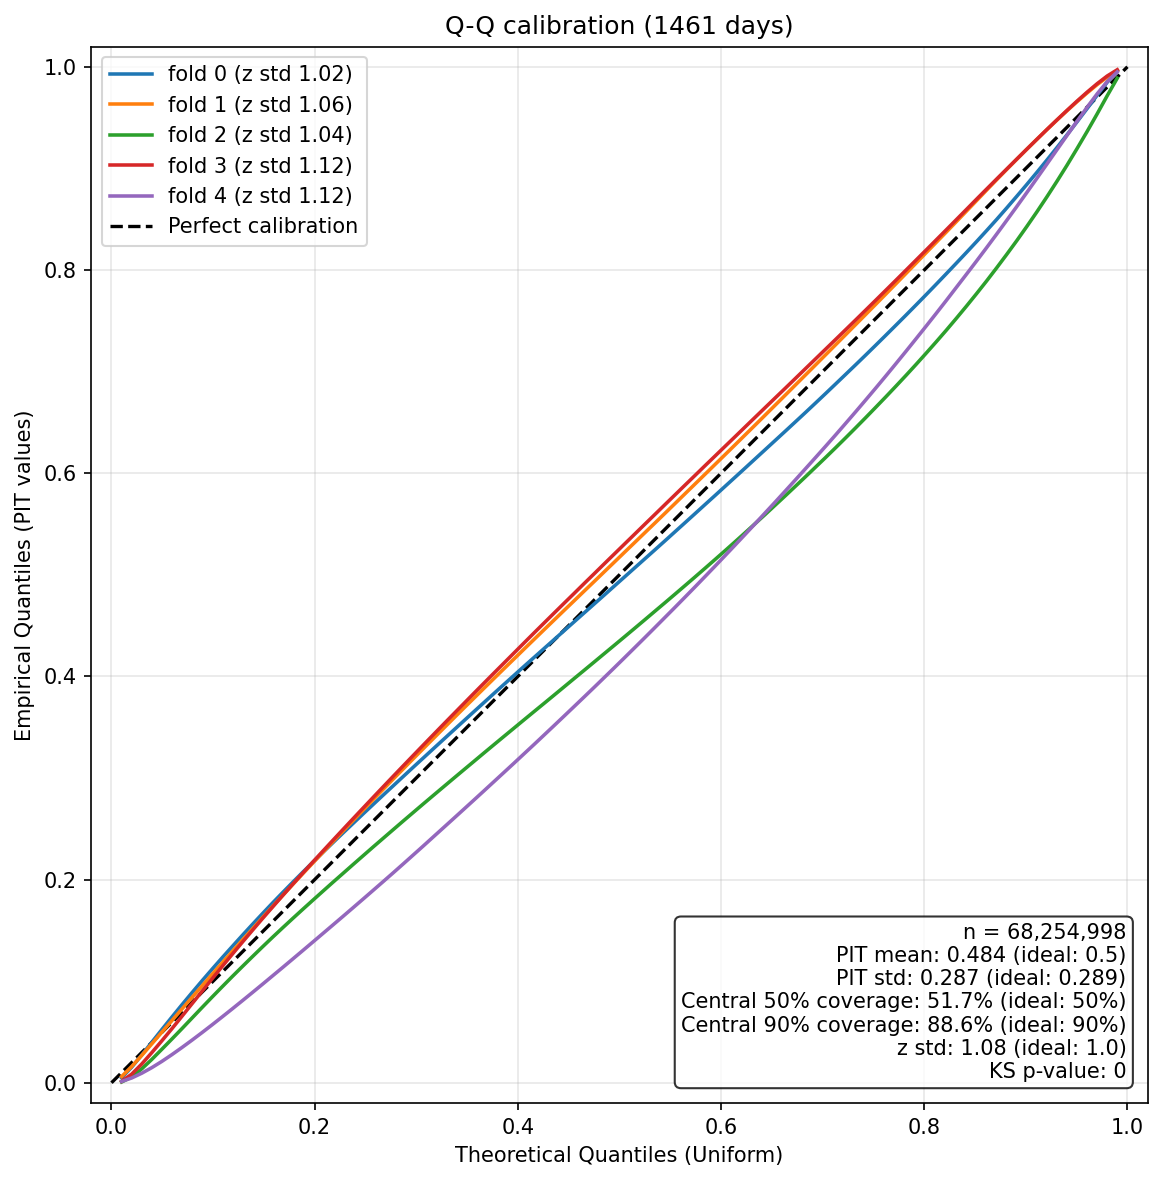
\includegraphics[width=0.46\textwidth]{images/results/tmax__qq_calibration__eval_cv__lbclip_wind.png}}\hfill%
\subfloat[2024 holdout, five-fold ensemble $\sigma$]{%

  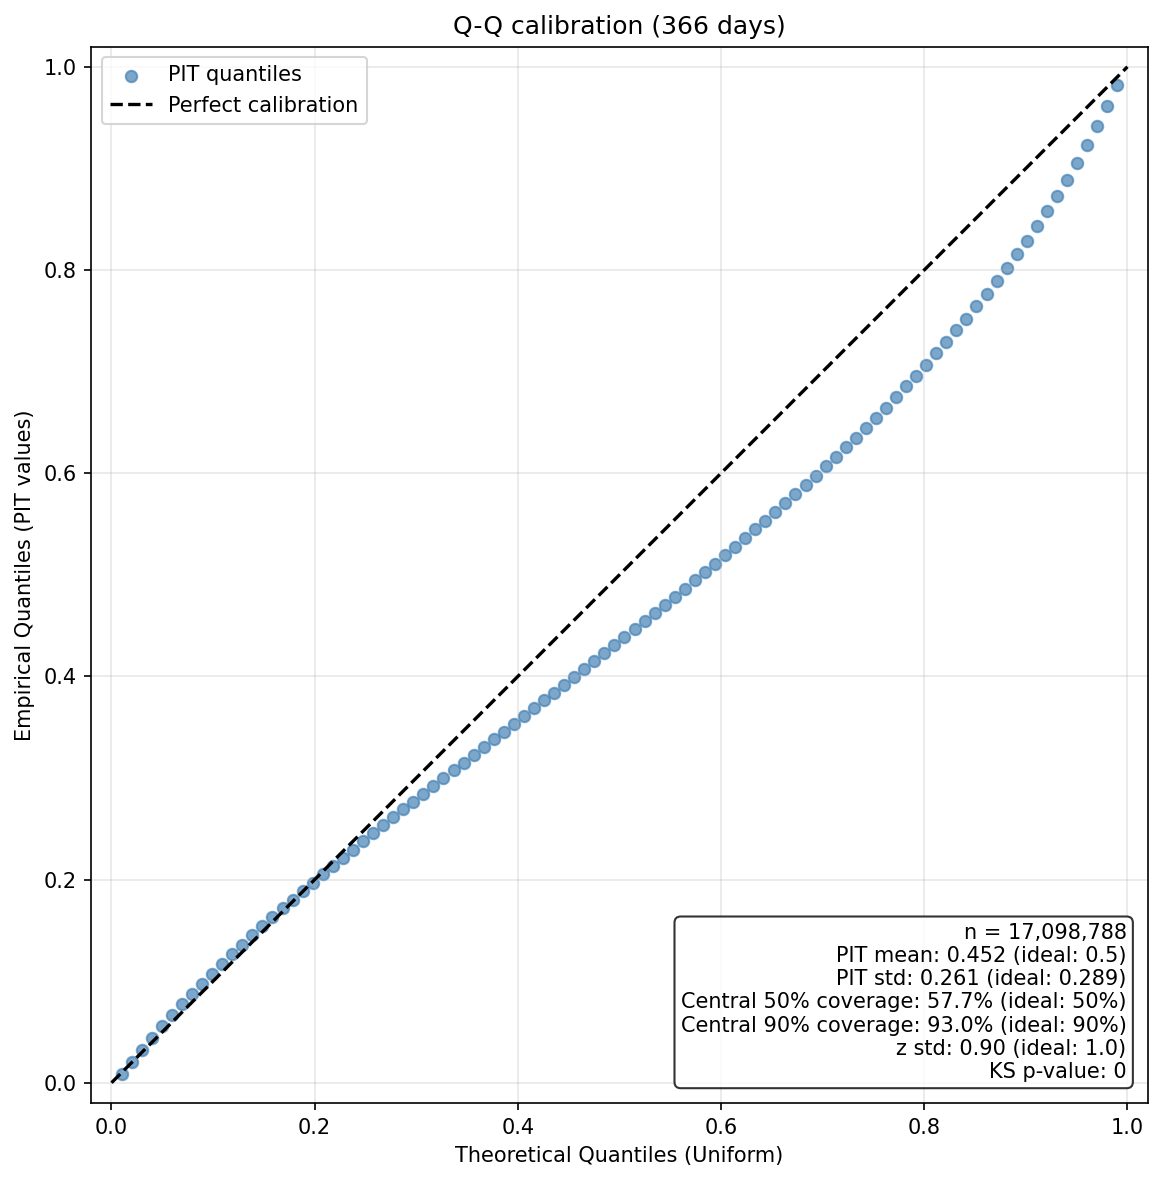
\includegraphics[width=0.46\textwidth]{images/results/tmax__qq_calibration__eval_2024__lbclip_wind.png}}

\caption[PIT calibration of the selected model across regimes]{PIT Q--Q calibration of \texttt{atm+wind-clip60} under both regimes. The CV panel draws one curve per fold, each fold scoring only the block it was held out from, so the spread between the curves is the disagreement between five separately trained models; the 2024 panel draws the single curve of the five-fold ensemble. }

\label{fig:single-tmax-pit}

\end{figure}



Over 2020--2023 the nominal $50\,\%$ and $90\,\%$ intervals capture $51.7\,\%$ and $88.6\,\%$ of the observations (\fref{fig:single-tmax-pit}). On 2024 they capture $57.7\,\%$ and $93.0\,\%$: the intervals are wider than the errors require, resulting in a conservative uncertainty estimate.



The PIT mean moves the same way, $0.48$ on the CV holdout against $0.45$ on 2024, which is the warm drift of \fref{fig:single-tmax-biasdrift} seen from the calibration side. The spread is still informative where it matters: it grows with the error it has to cover, at $r = 0.66$ on 2024 and $r = 0.55$ on the CV holdout. Across a range of more than $50\,^{\circ}\mathrm{C}$ the predicted density follows the observed one (\fref{fig:single-tmax-dist}); the exception is the warm tail, where every configuration puts too much probability above $30\,^{\circ}\mathrm{C}$.



\begin{figure}[H]

\centering

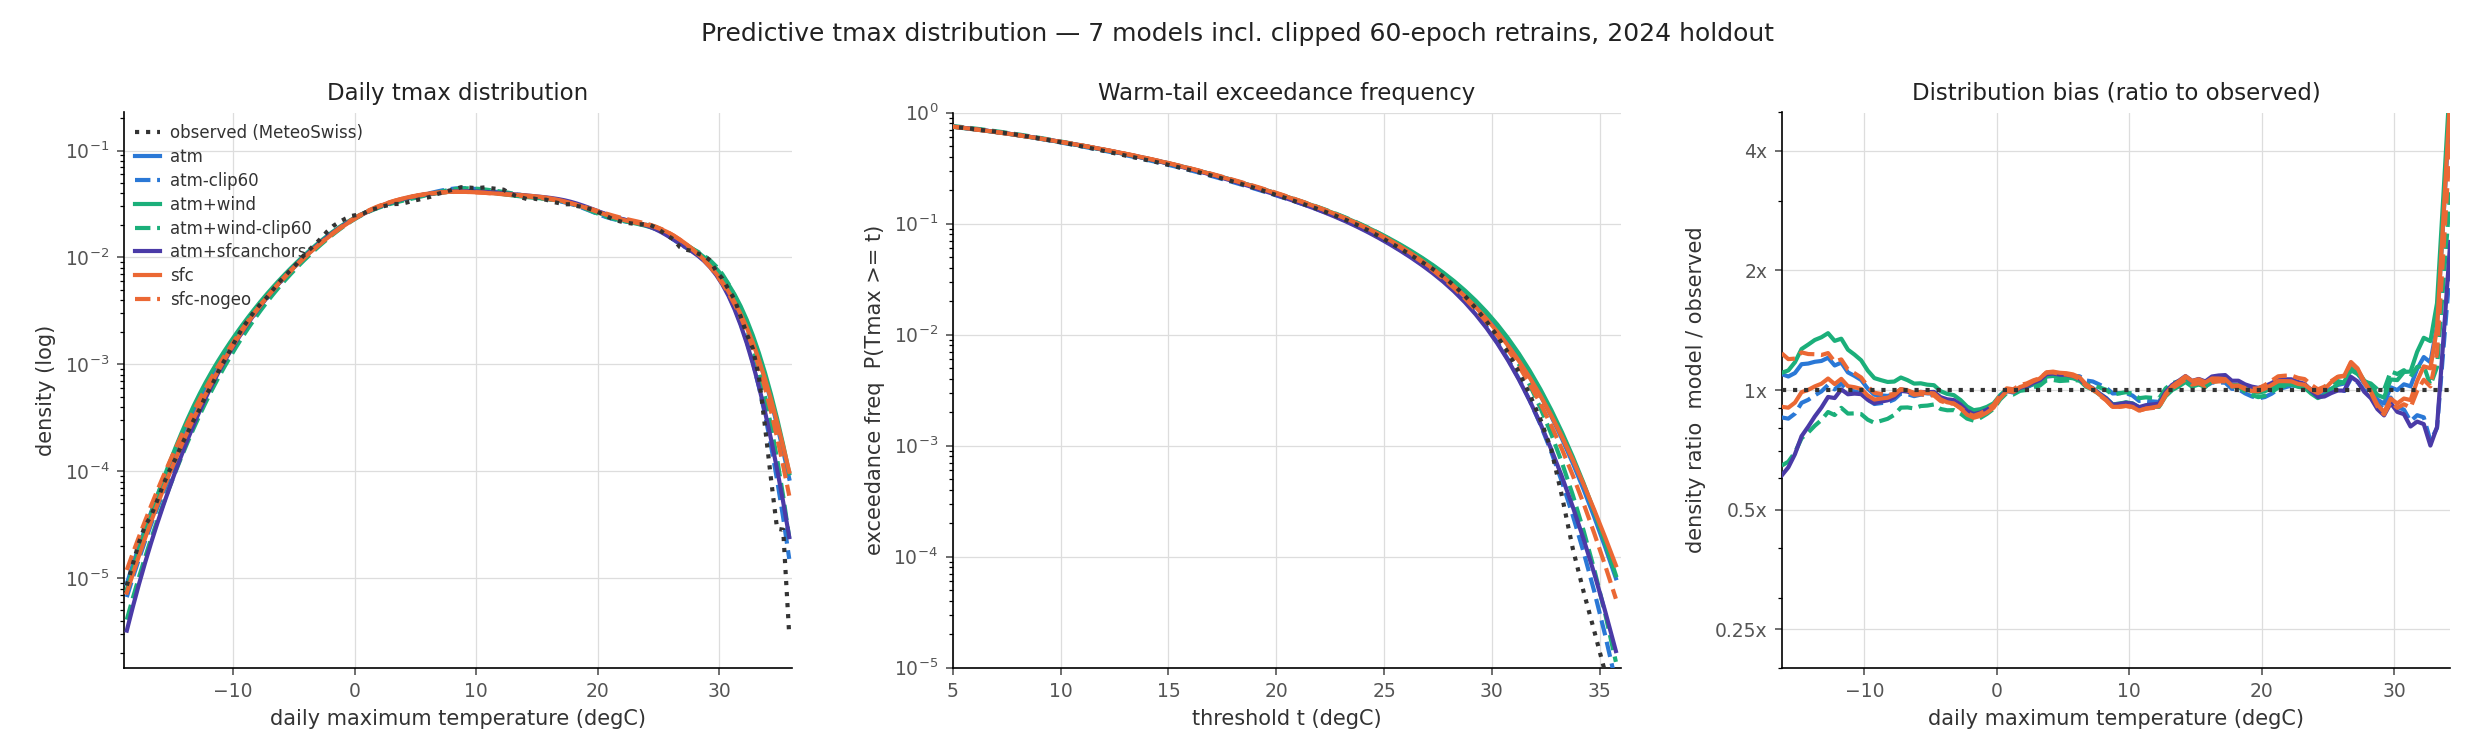
\includegraphics[width=\textwidth]{images/results/tmax__tmax_distribution_overlay_with_clip60_2024__tmax_model_comparison__ALL.png}

\caption[Predicted vs observed temperature distribution, 2024]{Predicted against observed daily-maximum temperature distribution over all points and days of 2024, for all seven models: log-density, warm-tail exceedance frequency, and the model-to-observed density ratio.}

\label{fig:single-tmax-dist}

\end{figure}

\subsection{Discussion}\label{subsec:single-tmax-discussion}



The atmospheric input generalises rather than merely fits the training years: all five atmospheric configurations hold or slightly improve their scores on 2024, a year no fold saw, relative to the CV holdout they were tuned against, while both surface configurations get worse (\fref{fig:single-tmax-slope}). An overfit model would degrade on unseen data, so this is the behaviour of a model that learnt something about the atmosphere rather than about the four particular years it was trained on. The advantage is not spread evenly: the surface input already tracks the fine-scale truth when that truth follows the coarse field, and it is mainly in the cold season, when the two decouple, that only the atmospheric input can keep up (\fref{fig:single-tmax-decoupling}). Against the predecessor project of \textcite{passos}, whose strongest configuration reaches a skill of $0.52$ with a surface input trained on ten years, the comparison is loose, since the evaluation years, the exact methodology and the training spans all differ. The more meaningful number is the internal comparison: on the CV holdout, moving from this work's own \texttt{sfc} baseline ($0.60$) to the selected atmospheric model ($0.70$) raises the skill by $0.10$.



Within the atmospheric input, the wind channels are a local rather than a global asset. Permutation importance ranks them near the bottom (\fref{fig:app-fi-sel-tmax}), yet under the extended training budget they buy the decisive margin of improvement exactly along the hardest-to-predict valley systems (\fref{fig:single-tmax-windgain}). 

Weather persists from one day to the next, so consecutive days do not carry independent information and a year of them is worth less than its calendar length suggests. Correcting for that persistence leaves 2024 with roughly $220$ effectively independent days rather than $366$ (\eref{eq:neff}). On that reduced sample the selected model's warm drift on 2024 is $+0.23\,^{\circ}\mathrm{C}$ with a $95\,\%$ interval of $[+0.16, +0.30]$, so it is a systematic offset and not a peculiarity of the evaluated year. The same test on the CV span returns $+0.08\,^{\circ}\mathrm{C}$ with an interval of $[+0.04, +0.12]$: the model is warm in both regimes, and what 2024 adds is a threefold amplification rather than the offset itself. Its amplitude is smaller than the model MAE so it is not a major flaw, but it is present.

The model selection itself is close rather than clear-cut: \texttt{atm+wind-clip60} is the most accurate model on every metric in both regimes, and it is the model we select, but \texttt{atm-clip60} would be the more robust choice for a use case that values stability over the last few hundredths of a degree. It transfers to 2024 almost without bias ($-0.02$ against $+0.23\,^{\circ}\mathrm{C}$), its calibration barely changes between the regimes, its five folds agree more closely (\fref{fig:app-sigma-decomposition}), and it does so with $95$ instead of $155$ channels.

Two weaknesses survive all of the seven configurations: the inner-Alpine valley floors and the over-predicted warm tail above $30\,^{\circ}\mathrm{C}$. Neither is fixed by picking a different model from this comparison; both need a lever this work did not pull. On training, that lever is already visible in the results here: doubling the epoch budget alone was worth more than any input modification achieved, and every model in this comparison still trained on only four years of data. Scaling both further, a longer schedule and more years, is the most direct, untested route to closing the valley-floor gap. The warm tail is a different kind of failure and will not close the same way; it needs a dedicated fix, such as post-processing the upper tail, rather than more training.

 One limit applies to everything in this chapter. The Gaussian head predicts each target point on its own (\sref{subsec:meth-gaussian}). Every map is therefore a field of per-point means, and every $\sigma$ is the spread at that point alone. Reading the maps and checking the calibration point by point is sound. What cannot be checked here is whether the errors have the right spatial structure, because the model never predicts how the error at one point relates to its neighbour. The between-fold spread of \fref{fig:app-sigma-decomposition} does not fill that gap: it measures how far the five folds disagree at each point, not how neighbouring points move together. In this work we have not studied this effect. Autoregressive sampling would settle it: coherent draws from the trained model, compared against the observed fine-scale variance~\cite{bruinsma2023arcnp}.

One design choice looks wrong in hindsight, and it concerns the domain rather than the model. The context grid extends well beyond the national border, but the loss is formed only at target points inside Switzerland (\sref{objective}): of the $88\,800$ points of the temperature lattice, only $46\,718$ ever carry a gradient. The model is therefore supervised only inside the Swiss border. The border region is therefore fitted with support that stops abruptly. Nothing constrains what the field does just outside, so the last kilometres inside the border are interpolated partly from grid cells whose behaviour was never scored. Extending the supervised area some way beyond the border or even the whole target set would have removed that asymmetry, and the data for it is available. Seen from the cost side the same choice is also wasteful, since roughly $47\,\%$ of the effort spent in the RBF layer and the elevation MLP goes to points that never enter the loss (\sref{subsec:meth-cost}).

\subsection{Conclusion}\label{subsec:single-tmax-conclusion}



This chapter answers the two questions it set out to ask (\sref{sec:intro-questions}) for temperature. Meteorologically relevant features do improve accuracy and calibration over surface data: atmospheric input beats surface input on every metric, keeps improving rather than degrading on the unseen 2024 year, and the selected model, \texttt{atm+wind-clip60}, reaches a skill of $0.71$ and a MAE of $1.03\,^{\circ}\mathrm{C}$ with a small, well-behaved warm bias as its only significant caveat.


The model also learns physically meaningful structure rather than acting as a trained interpolator: it relies on lower-tropospheric temperature at the hours a warm front or a clear midday sky would matter, not on scaffold or coordinate channels, and this reliance is what lets it, unlike the surface models, generalise better to weather it never trained on. The remaining weaknesses are the MAE over the inner-Alpine valley floors, the warm tail, and the cold-season decoupling of surface-driven inputs.



\section{Precipitation Model}\label{sec:single-precipitation}




\subsection{Model Variants}\label{subsec:single-precip-variants}

In the presented models, two axes are studied: the training objective and the input feature set. Three runs share the
atmospheric input of the temperature study and differ only in the objective they minimise:
\texttt{precip-NLL}, \texttt{precip-CRPS} and \texttt{precip-FT-CRPS}. \texttt{precip-WIND} adds the
wind components to that same atmospheric input.

\texttt{precip-SFC-TP} replaces the atmospheric inputs with a pure surface
input including ERA5-Land total precipitation and daily-maximum $2\,\mathrm{m}$ temperature. \tref{tab:single-precip-variants} lists all five with the model names used throughout.

In this section the reference baseline is the bilinearly interpolated ERA5-Land total precipitation. To match the evaluation window of the observed target, the reference is rebuilt on a $06\,\mathrm{UTC}$ to $06\,\mathrm{UTC}$ window (\sref{sec:data-preprocessing}). The input channel of \texttt{precip-SFC-TP} keeps the $00\,\mathrm{UTC}$ window all atmospheric models were trained on.


\begin{table}[H]
\centering
\caption[The five precipitation runs]{The five precipitation runs. All share the architecture of
\sref{sec:meth-architecture}, the Bernoulli--Gamma head of \sref{subsec:meth-likelihoods} and the
setup of \tref{tab:meth-training-setup}; \texttt{precip-FT-CRPS} is a warm start run from the trained
\texttt{precip-NLL} model with the objective function based on CRPS.}
\label{tab:single-precip-variants}
\footnotesize
\begin{tabular}{|>{\raggedright\arraybackslash}p{2.8cm}|>{\raggedright\arraybackslash}p{5.2cm}|>{\raggedright\arraybackslash}p{3.2cm}|>{\raggedright\arraybackslash}p{1.0cm}|}
\hline
\textbf{Model name} & \textbf{Context input} & \textbf{Objective} & \textbf{Chan.} \\
\hline
\texttt{precip-NLL} & ERA5 pressure-level $z$, $t$, $q$ on six levels at five hours, plus scaffold &
mixture NLL, \mbox{\eref{eq:bg-ll}} & 95 \\
\hline
\texttt{precip-CRPS} & as \texttt{precip-NLL} & sampled CRPS, \mbox{\eref{eq:crps}} & 95 \\
\hline
\texttt{precip-FT-CRPS} & as \texttt{precip-NLL} & NLL, then $10$ epochs of CRPS & 95 \\
\hline
\texttt{precip-WIND} & as \texttt{precip-NLL}, with the wind components $u$ and $v$ added & mixture NLL & 155 \\
\hline
\texttt{precip-SFC-TP} & ERA5-Land total precipitation and daily-maximum $2\,\mathrm{m}$ temperature, plus
scaffold & mixture NLL & 7 \\
\hline
\end{tabular}
\end{table}



\subsection{Headline Metrics}\label{subsec:single-precip-headline}

\fref{fig:single-precip-slope} and \fref{fig:single-precip-slope-skill} plot each run from its CV-holdout score to its 2024 score. The values themselves are in \tref{tab:single-precip-headline}.

Every quantity plotted for the runs is a closed-form functional of the fitted Bernoulli--Gamma
distribution, evaluated per point-day: the predictive mean $\rho\alpha/\beta$ for the errors and the
rank correlation, $P(Y \geq 1\,\mathrm{mm})$ for occurrence and
$E[Y \mid Y \geq 1\,\mathrm{mm}]$ for intensity; the two skill scores combine these with the same
ERA5-Land reference the grey line carries. Thresholds enter only as events: $1\,\mathrm{mm}$ for
occurrence and intensity, the four category edges for the RPSS and never as a wet/dry decision
on the prediction. All statistics pool days and points together. 
\begin{figure}[H]
\centering
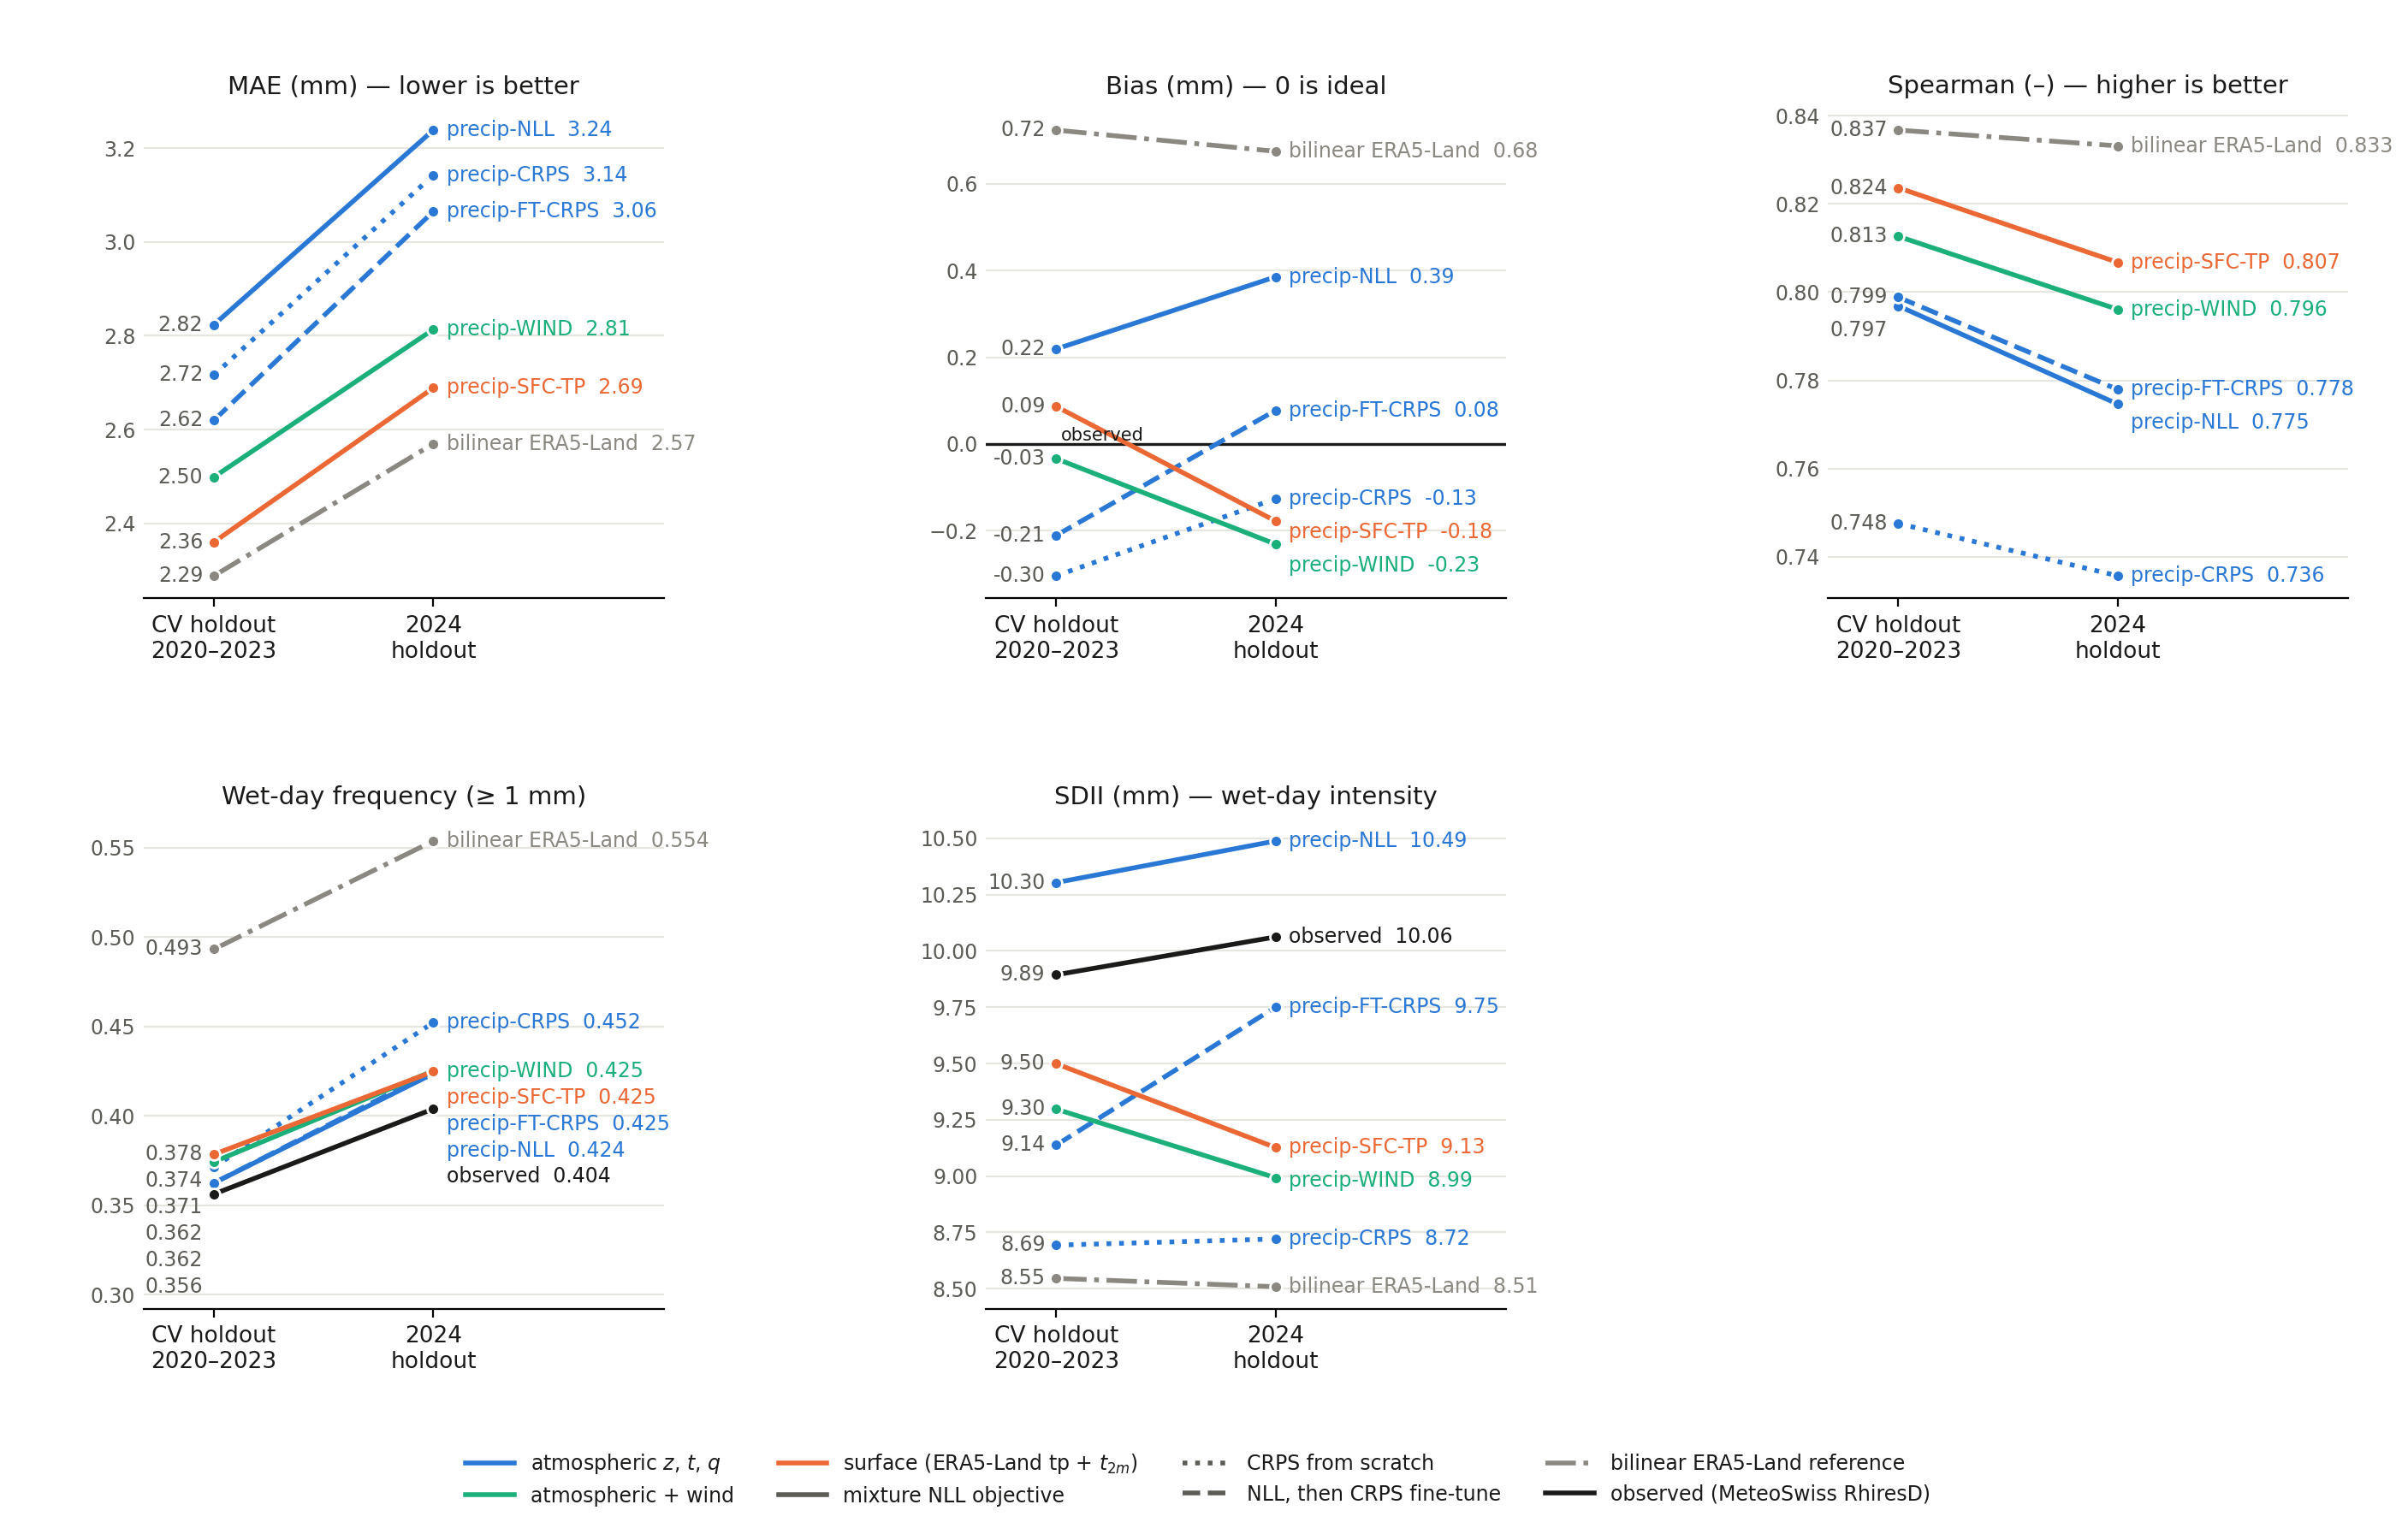
\includegraphics[width=\textwidth]{images/precip_regime_slope.png}
\caption[Accuracy of the precipitation runs, CV to 2024]{The scores of the five
precipitation runs from the CV holdout to the unseen year: the two error measures and the rank
correlation on the top row, occurrence and wet-day intensity below. Colour encodes the input family
and line style the training objective; the bilinear ERA5-Land reference is the grey line and the
observed target the black one.}
\label{fig:single-precip-slope}
\end{figure}

\begin{figure}[H]
\centering
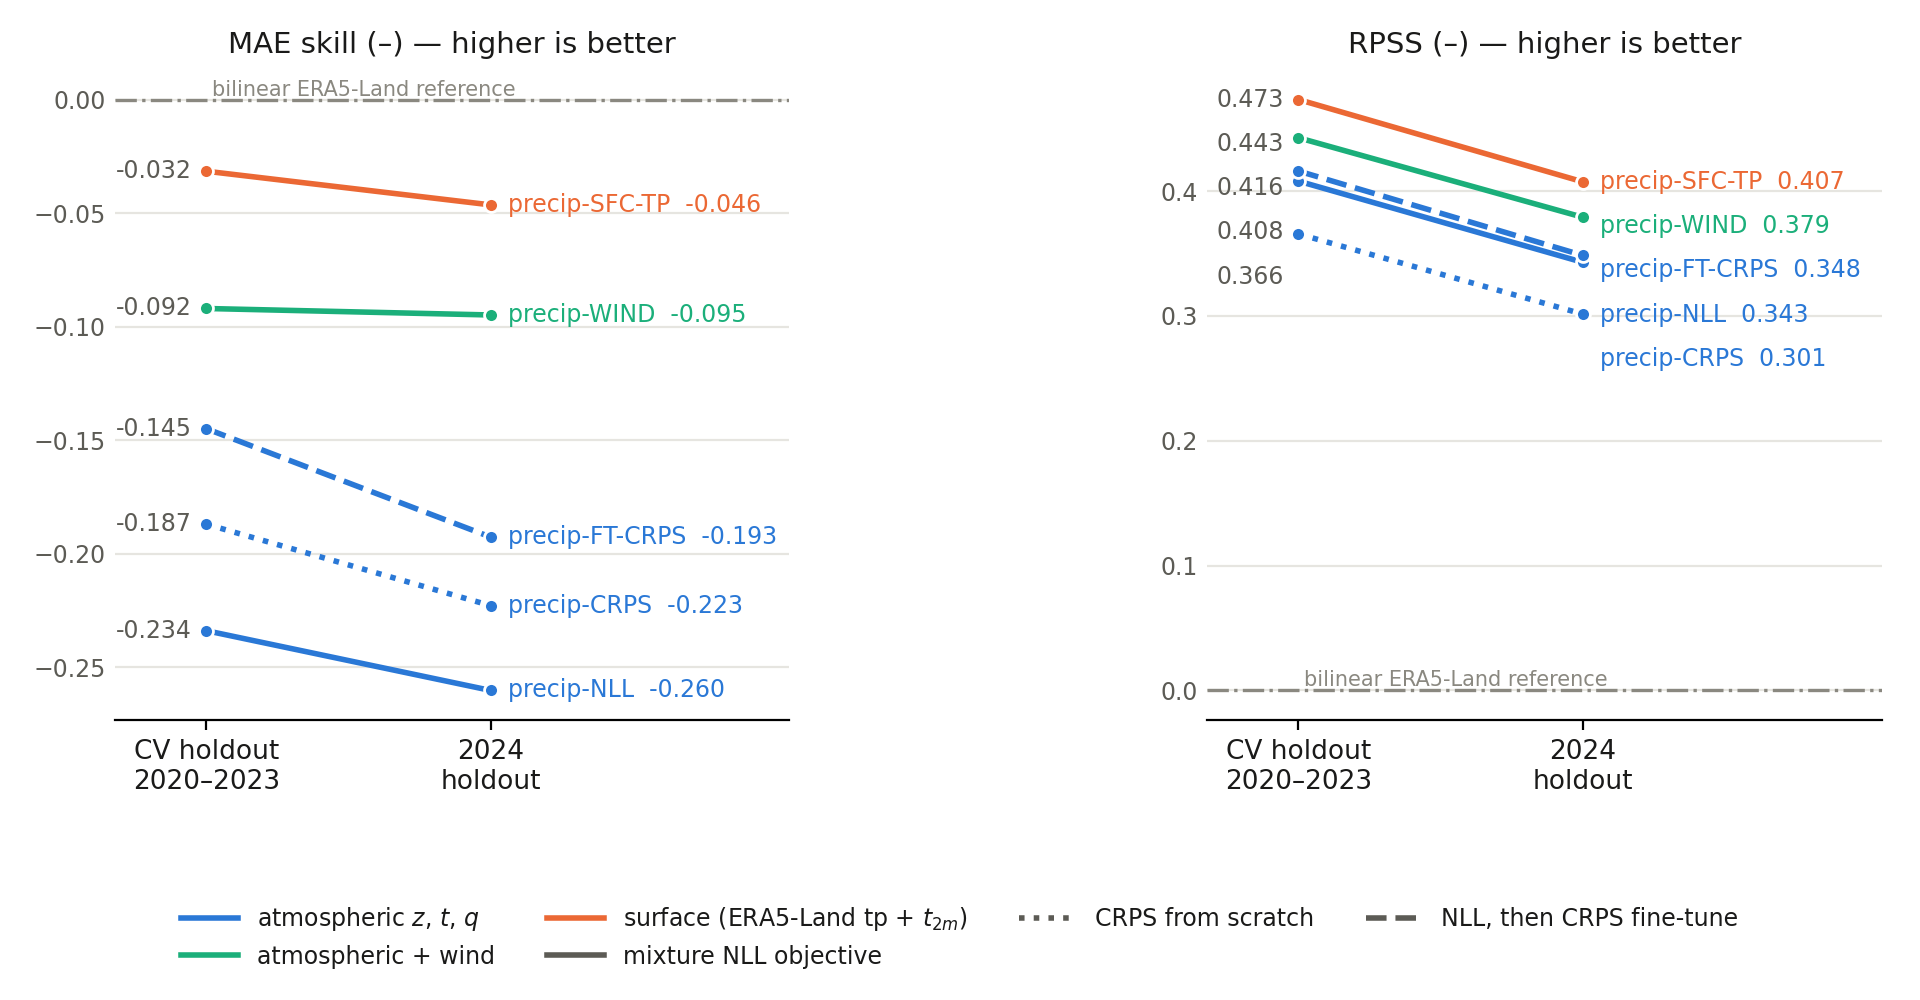
\includegraphics[width=0.8\textwidth]{images/precip_regime_slope_skill.png}
\caption[Skill of the precipitation runs, CV to 2024]{The two skill scores of the five runs over the
same two regimes, on the conventions of \fref{fig:single-precip-slope}. Both are defined against the
bilinear ERA5-Land reference, so the reference is the zero rule: the MAE skill of
\eref{eq:mae-skill} is negative for every run in both regimes, while the RPSS of \eref{eq:rpss} is
strongly positive for all of them. The two agree on the ranking apart from the two weakest runs, which swap places.}
\label{fig:single-precip-slope-skill}
\end{figure}

Together the two figures show why precipitation is complex to evaluate. In \fref{fig:single-precip-slope} the two error measures, MAE and rank correlation, favour the reference, while the two physical measures, occurrence and intensity, favour the downscaling runs. \fref{fig:single-precip-slope-skill} turns that split into a disagreement of sign: scored against the same reference, the MAE skill of \eref{eq:mae-skill} is negative for every run in both regimes while the RPSS of \eref{eq:rpss} is strongly positive for all of them. Studying a headline metric is therefore not enough to make a statement about model performance, and a more detailed analysis is needed to understand the strengths and weaknesses of each run.


\begin{table}[H]
\centering
\caption[Headline precipitation metrics, CV holdout vs 2024]{Headline metrics of the five
precipitation runs and of the bilinear ERA5-Land reference, in both regimes. MAE and bias are in
$\mathrm{mm\,day^{-1}}$; $r_{S}$ is the pooled Spearman rank correlation; R01 is the predicted-over-observed
wet-day frequency, ideal $1$; SDII bias is the predicted minus observed wet-day intensity in
$\mathrm{mm}$; RPSS is the five-category ranked probability skill against the same reference
(\eref{eq:rpss}), zero for the reference by definition.}
\label{tab:single-precip-headline}
\footnotesize
\setlength{\tabcolsep}{3.5pt}
\begin{tabular}{|l|cc|cc|cc|cc|cc|cc|}
\hline
& \multicolumn{2}{c|}{\textbf{MAE}} & \multicolumn{2}{c|}{\textbf{Bias}} &
\multicolumn{2}{c|}{$\boldsymbol{r_{S}}$} & \multicolumn{2}{c|}{\textbf{R01}} &
\multicolumn{2}{c|}{\textbf{SDII bias}} & \multicolumn{2}{c|}{\textbf{RPSS}} \\
\textbf{Run} & CV & 2024 & CV & 2024 & CV & 2024 & CV & 2024 & CV & 2024 & CV & 2024 \\
\hline
\texttt{precip-NLL}     & $2.82$ & $3.24$ & $+0.22$ & $+0.39$ & $0.797$ & $0.775$ & $1.017$ & $1.049$ & $+0.41$ & $+0.43$ & $0.408$ & $0.343$ \\
\hline
\texttt{precip-CRPS}    & $2.72$ & $3.14$ & $-0.30$ & $-0.13$ & $0.748$ & $0.736$ & $1.042$ & $1.120$ & $-1.20$ & $-1.34$ & $0.366$ & $0.301$ \\
\hline
\texttt{precip-FT-CRPS} & $2.62$ & $3.06$ & $-0.21$ & $+0.08$ & $0.799$ & $0.778$ & $1.017$ & $1.052$ & $-0.76$ & $-0.31$ & $0.416$ & $0.348$ \\
\hline
\texttt{precip-WIND}    & $2.50$ & $2.81$ & $-0.03$ & $-0.23$ & $0.813$ & $0.796$ & $1.051$ & $1.053$ & $-0.60$ & $-1.07$ & $0.443$ & $0.379$ \\
\hline
\texttt{precip-SFC-TP}  & $2.36$ & $2.69$ & $+0.09$ & $-0.18$ & $0.824$ & $0.807$ & $1.064$ & $1.052$ & $-0.40$ & $-0.94$ & $0.473$ & $0.407$ \\
\hline
Reference               & $2.29$ & $2.57$ & $+0.72$ & $+0.68$ & $0.837$ & $0.833$ & $1.385$ & $1.371$ & $-1.35$ & $-1.55$ & $0.000$ & $0.000$ \\
\hline
\end{tabular}
\end{table}

\tref{tab:single-precip-headline} collects the same scores as values, and adds the bias, which the slope panels do not carry. The two error measures split from the two physical ones: the reference has the lowest MAE ($2.29$ against $2.36$ for the best run) and the highest rank correlation, yet it calls a wet day $38\,\%$ too often where no run departs from the observed frequency by more than $7\,\%$ on the training span; on the unseen year only \texttt{precip-CRPS} drifts further, to $+12\,\%$. \texttt{precip-SFC-TP} is the strongest run on almost every column and \texttt{precip-CRPS} the weakest, with \texttt{precip-FT-CRPS} recovering most of what training on the CRPS from scratch gives away. The ordering is reproduced on the unseen year: nearly every column deteriorates, the reference included, so 2024 is a harder year rather than one the models fail on. The exception is the wet-day intensity, where only \texttt{precip-NLL} runs wetter than observed and every other run, like the reference, runs dry.


\begin{figure}[H]
\centering
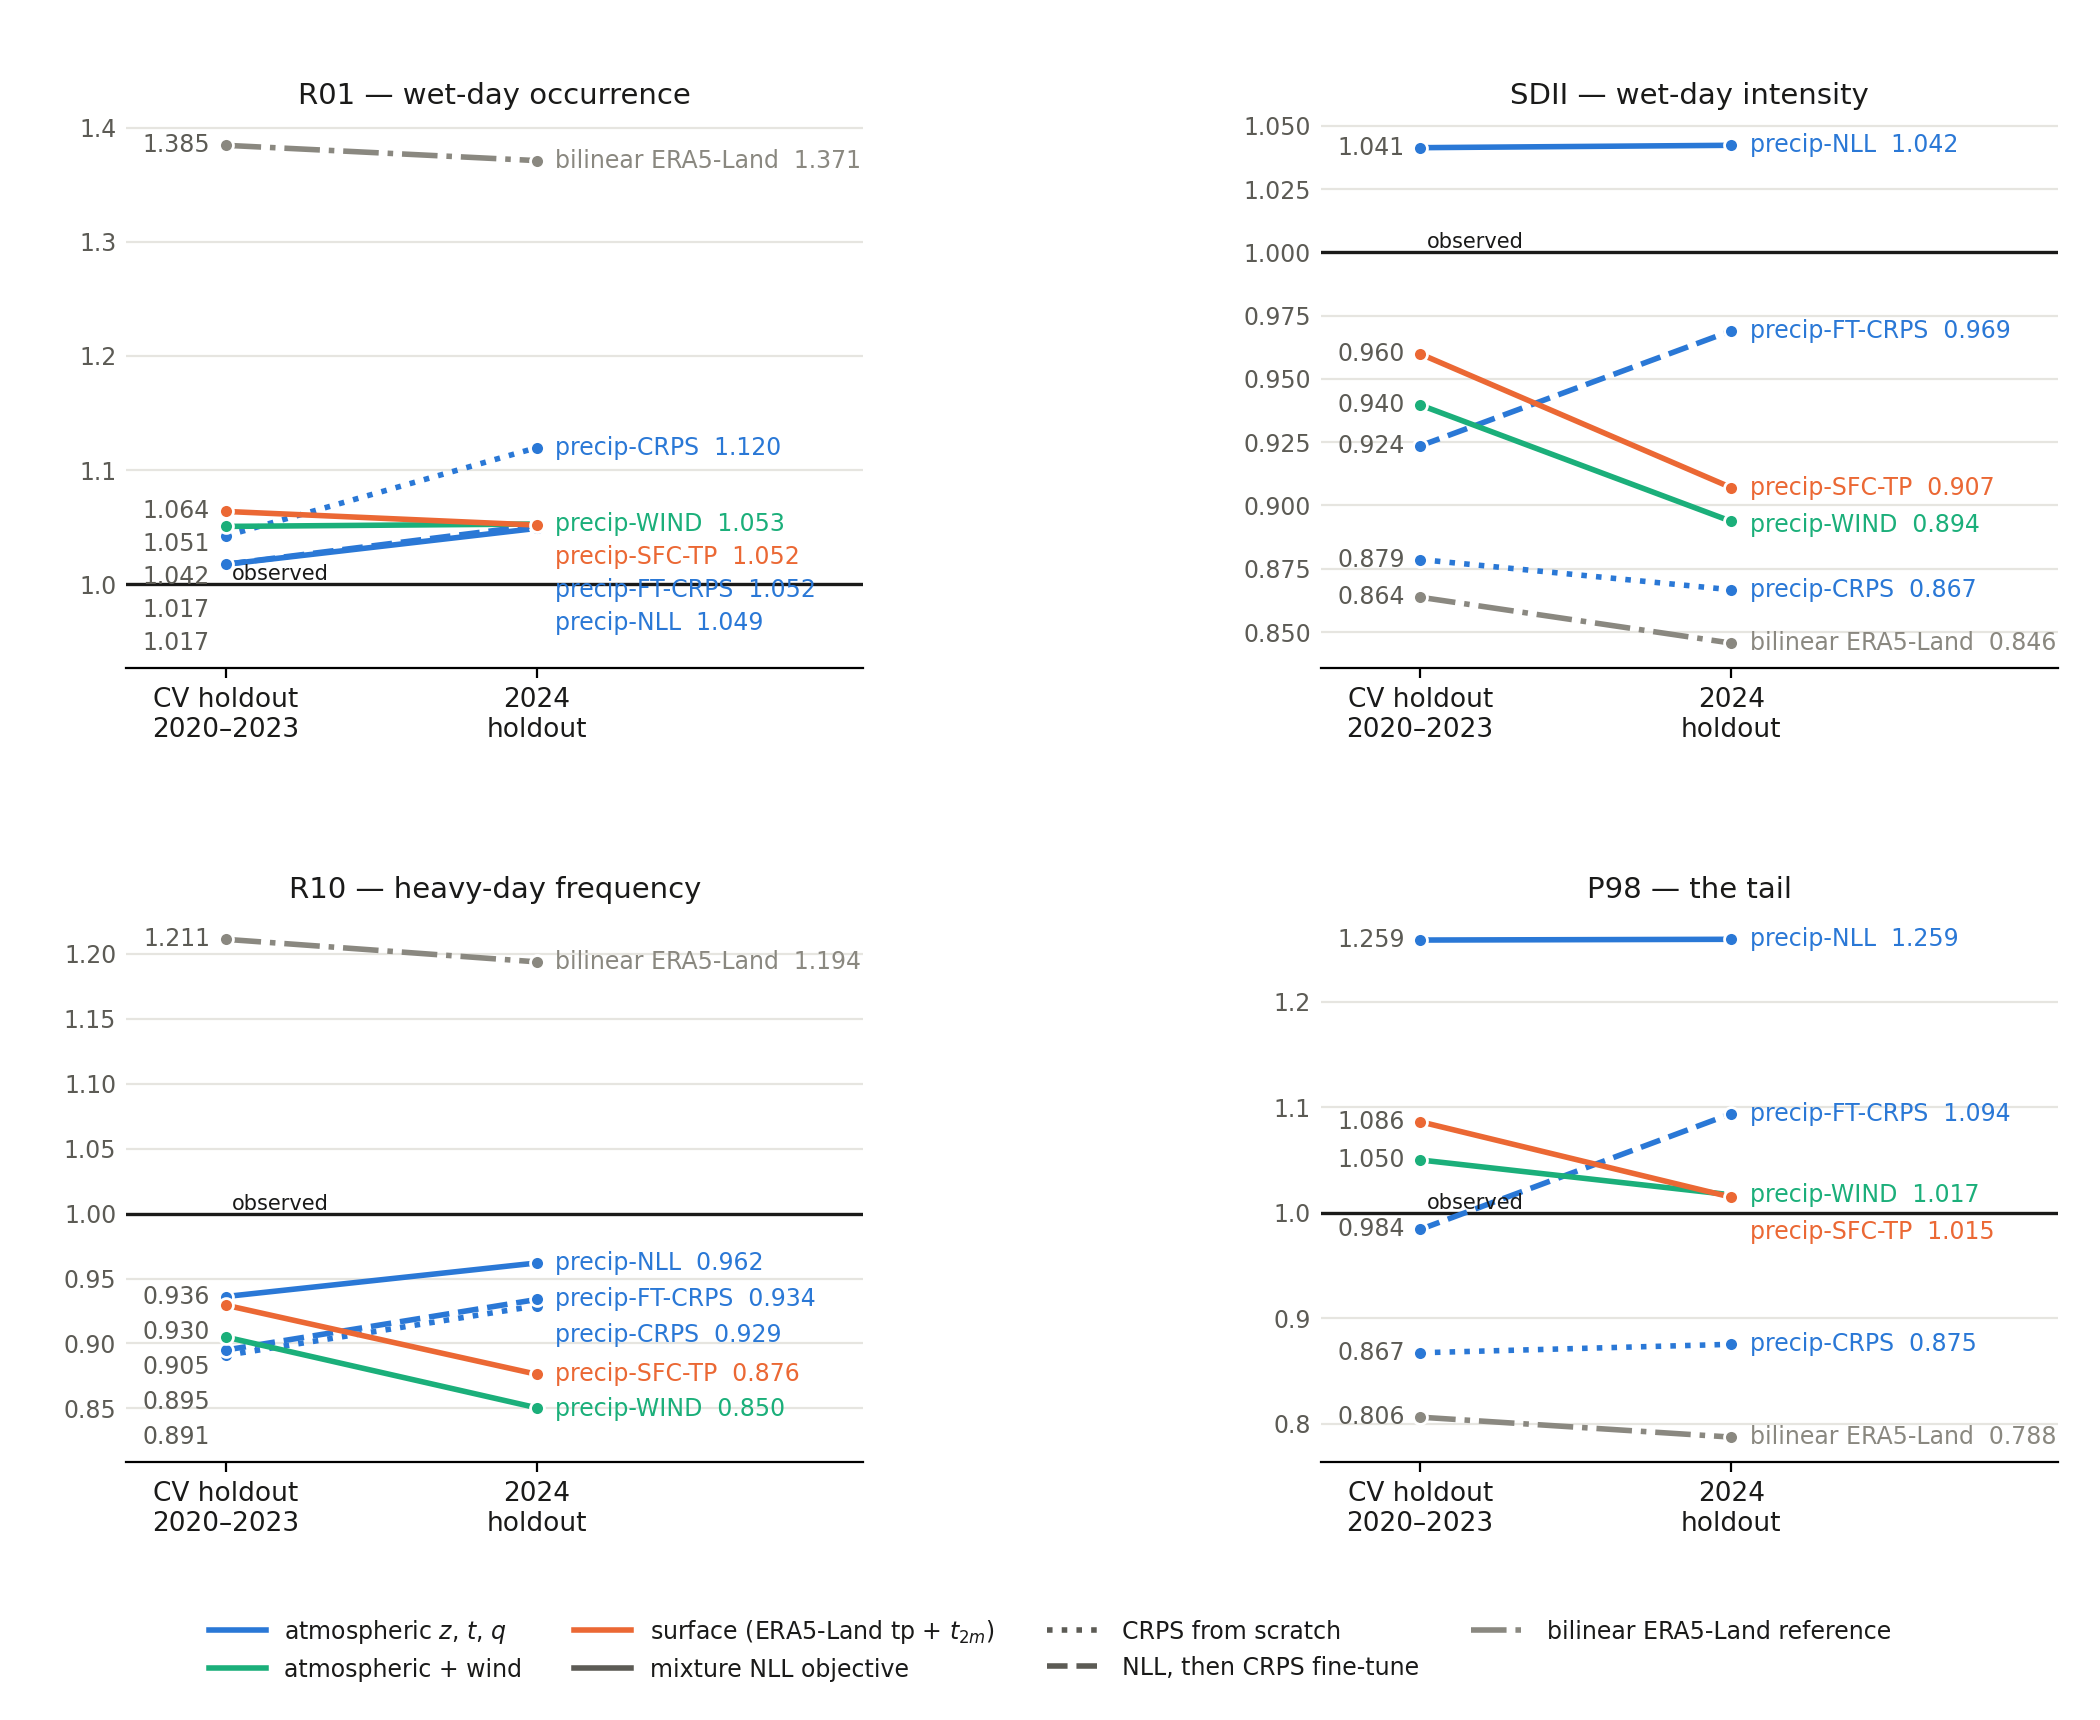
\includegraphics[width=\textwidth]{images/precip_regime_slope_indices.png}
\caption[The four physical precipitation indices]{The four physical precipitation indices of
\tref{tab:app-metrics-overview} from the CV holdout to the unseen year, on the conventions of
\fref{fig:single-precip-slope}: occurrence (R01), typical intensity (SDII), heavy-day frequency
(R10) and the tail (P98). Every panel is a predicted-over-observed ratio.}
\label{fig:precip-indices}
\end{figure}
\fref{fig:precip-indices} carries occurrence and intensity into the heavy categories, adding the heavy-day frequency R10 and the tail P98 to the two indices already seen. Each is a predicted-over-observed ratio, so one is a perfect match in every panel. R01 makes the occurrence gap quantitative, the reference overshooting the observed wet-day frequency by $+38\,\%$ where no run departs by more than $+7\,\%$ on the CV holdout, and heavy-day frequency behaves the same way, the reference overshooting R10 by $+21\,\%$ while every run undershoots it by between $6$ and $11\,\%$. The extreme tail is the one index where the reference beats a run: it undershoots P98 by $-19\,\%$, \texttt{precip-NLL} overshoots it by $+26\,\%$. On the unseen year the reference behaves much as it does on the training span, and so do \texttt{precip-SFC-TP} and \texttt{precip-WIND}; the three objective variants improve on R10 while \texttt{precip-FT-CRPS} drifts back towards \texttt{precip-NLL} in SDII and P98.


Neither the raw measures nor the indices provide a clear response to which model performs best: 
different runs score best on different indices, and on two of them, MAE and rank correlation, the reference beats every run.

\subsection{Skill by Intensity Category}\label{subsec:single-precip-categories}

Precipitation is a harder downscaling target than temperature, and the reason lies in how the
observations are distributed rather than in the models. Over the CV holdout $52\,\%$ of point-days
are dry and a further $36\,\%$ stay below $10\,\mathrm{mm}$, while the two heaviest categories
together account for under $1\,\%$. Any score pooled over that distribution is therefore decided by
days on which little happens, whereas the days a downscaling product is wanted for sit in a tail
thin enough that the estimates there rest on few events and carry a correspondingly wide spread.
In \fref{fig:single-precip-categories} the brier scores for the different intensity categories are reported.

\begin{figure}[H]
\centering
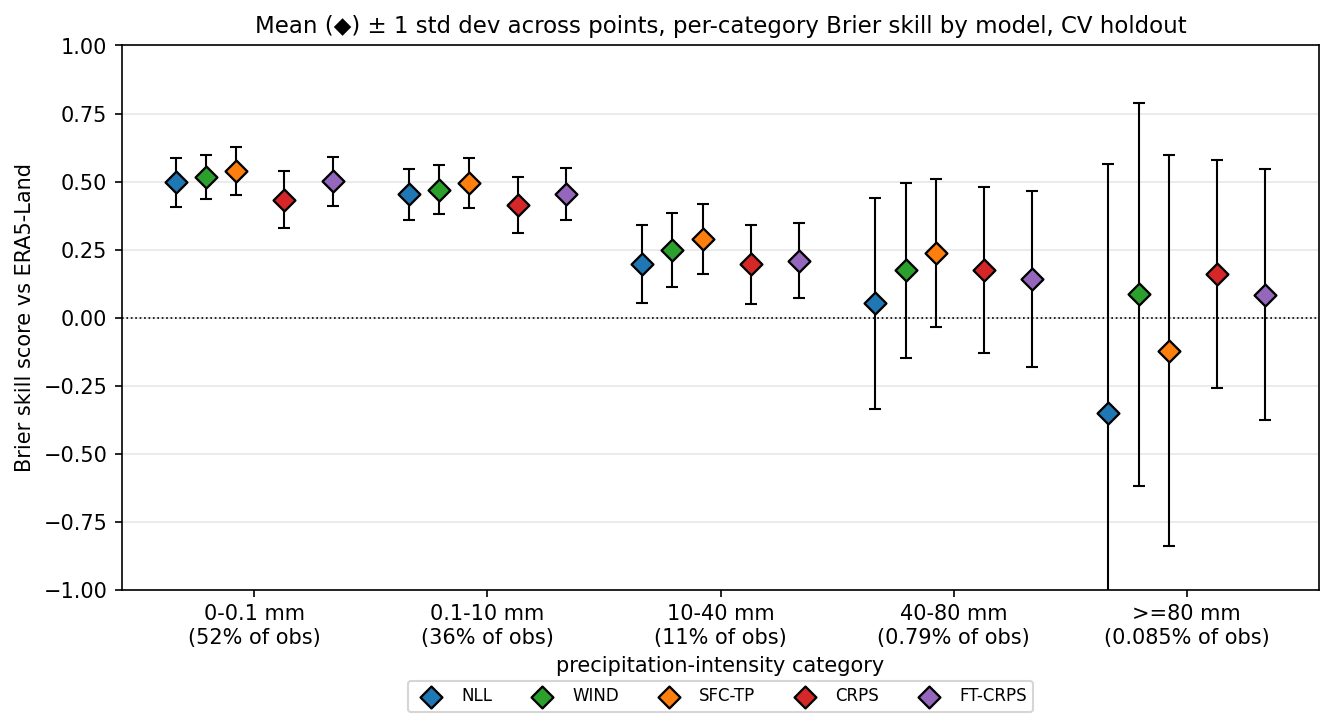
\includegraphics[width=\textwidth]{images/results/precip__bss_category_comparison__precip_processing_comparison__ALL.png}
\caption[Brier skill by intensity category]{Brier skill score against the bilinear ERA5-Land
reference, by intensity category evaluated on CV holdout. Positive means
the run places that category's probability better than the reference. Every grid point first gets its own
Brier skill score then we average over the points. The diamond is then the mean of those per-point skills over the domain and the
whisker their $\pm1$ standard deviation. The whisker is therefore a spatial spread, not a standard
error.}
\label{fig:single-precip-categories}
\end{figure}

Read by intensity category, three things follow. Almost all of the pooled skill is earned in the two categories that carry $88\,\%$ of point-days, where all five models sit close together between $+0.41$ and $+0.54$ and clearly beat the reference. Skill then falls monotonically with intensity, and the estimate loses significance as it goes: by $\geq 80\,\mathrm{mm}$ the spread across grid points is several times the mean for every model. The ordering shifts in the two heaviest categories, most of all in the last. \texttt{precip-SFC-TP}, first almost everywhere else, and \texttt{precip-NLL} both fail there, while \texttt{precip-CRPS} holds the best tail on both mean and spread and \texttt{precip-FT-CRPS} is the best compromise, keeping nearly all of \texttt{precip-WIND}'s skill in the frequent categories and nearly all of \texttt{precip-CRPS}'s tail robustness. Because RPSS weights by frequency and that category is $0.085\,\%$ of point-days, none of it registers in \tref{tab:single-precip-selection}: reading the two together is what separates a model that is uniformly good from one that is good where the days are.


\fref{fig:single-precip-spatial-categories} visualises this comparison for the two best balanced models \texttt{precip-SFC-TP} and \texttt{precip-FT-CRPS}. The observed frequencies are put next to the reference and the model frequencies and the skill column presents the spatial skill distribution.
\begin{figure}[p]
\centering
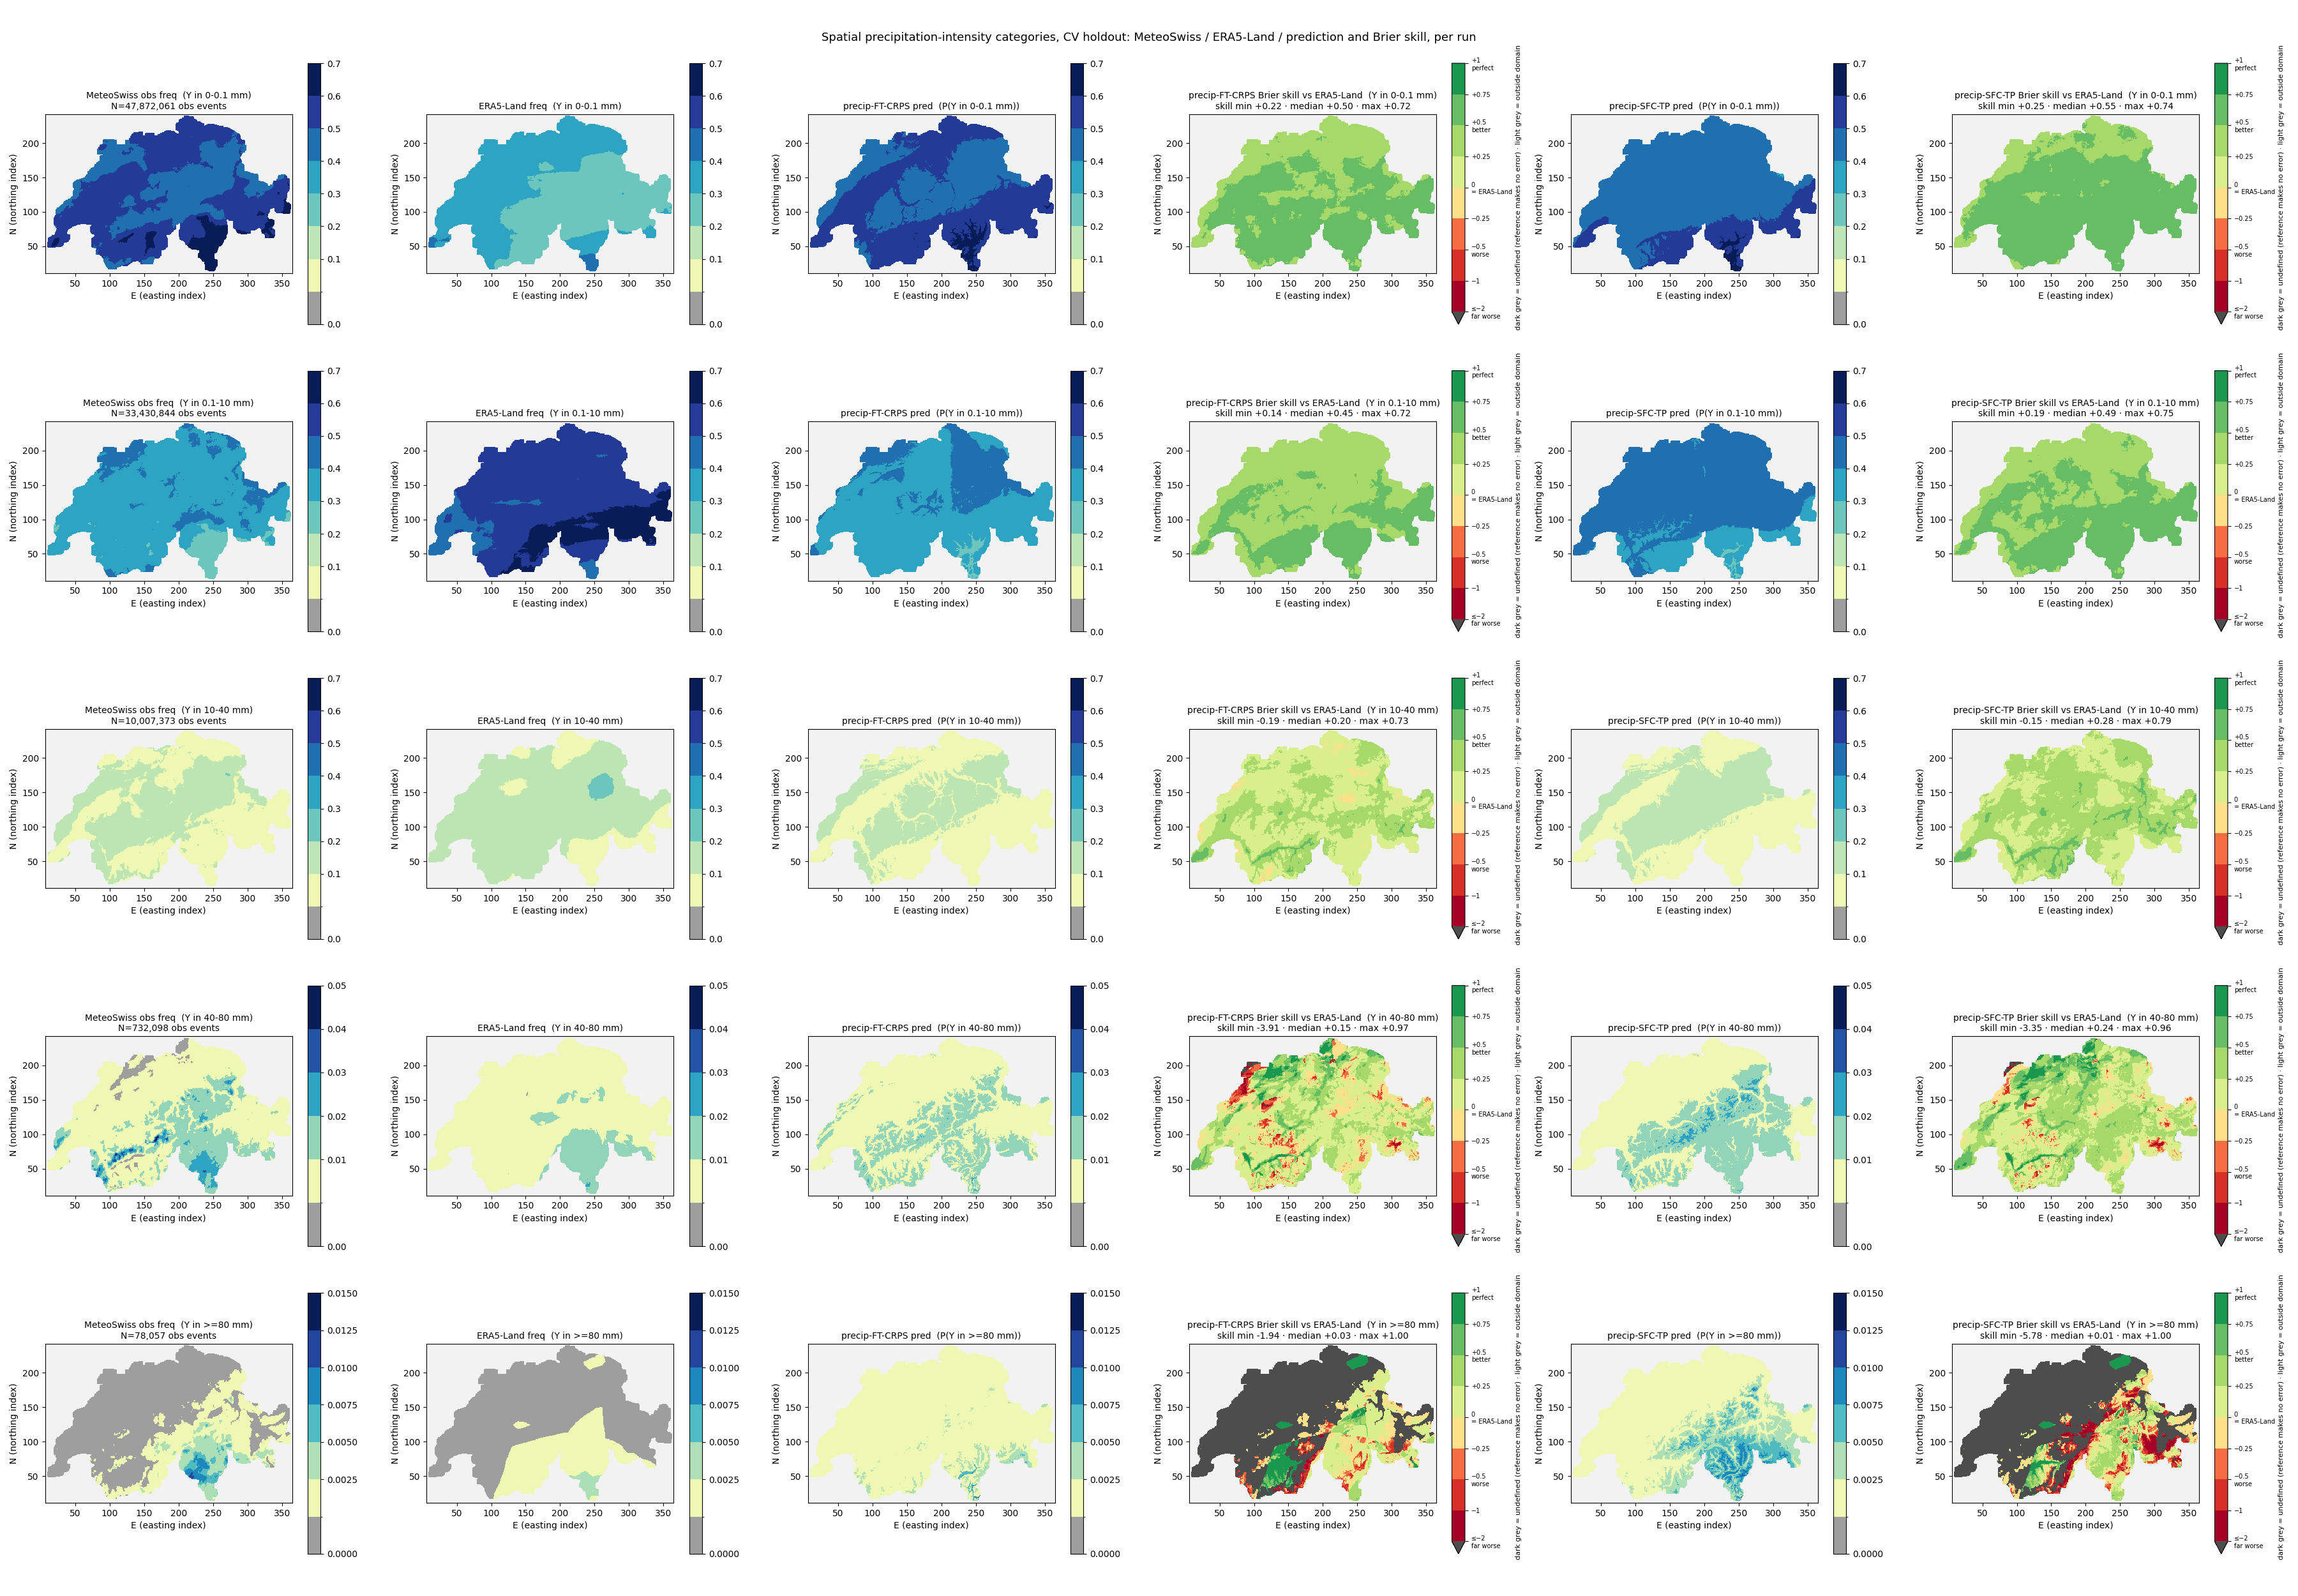
\includegraphics[angle=90,origin=c,width=\linewidth,height=0.92\textheight,keepaspectratio]{images/results/precip__category_spatial_pair__precip_processing_comparison__ALL.png}
\caption[Spatial distribution of Categorical Brier Skill score]{Spatial distribution of Brier skill by rain category for fine-tuned and the surface run. Rows Intensity categories, Columns from left to right observed frequency, reference frequency, FT-CRPS frequency, FT-CRPS Skill, SFC frequency, SFC skill.}
\label{fig:single-precip-spatial-categories}
\end{figure}


In the first three categories (dry days $<0.1\,\mathrm{mm}$, drizzle $0.1$--$10\,\mathrm{mm}$ and
ordinary rain days $10$--$40\,\mathrm{mm}$) both models perform well, and \texttt{precip-SFC-TP} is
slightly ahead on the numbers, its median skill exceeding that of \texttt{precip-FT-CRPS}. The spatial fields separate them more than the numbers do.
\texttt{precip-FT-CRPS} resolves the terrain, its frequency bands following the Alpine ridges and
valleys, whereas
\texttt{precip-SFC-TP} stays closer to the reference's own spatial distribution.

The two heavy categories behave differently from each other, and only the heaviest separates the
runs significantly. Between $40$ and $80\,\mathrm{mm}$ \texttt{precip-SFC-TP} is still ahead. Above $80\,\mathrm{mm}$ the ordering
reverses: the two median skills over grid points are effectively tied at $+0.01$ and $+0.03$, but the
surface run's worst point falls to $-5.78$ where the fine-tuned run holds $-1.94$. 
\texttt{precip-SFC-TP} predicts extreme-event frequencies at roughly the observed magnitude but
spreads them over large areas that never observe such events, so where it is wrong it is wrong by a
wide margin; \texttt{precip-FT-CRPS} stays conservative and keeps its losses bounded. Due to the sparsity of observed points in this category such patches are
difficult to avoid. No terrain feature explains their placement; the error along the Jura ridge is
more likely a domain-edge effect, since the loss is formed only at target points inside Switzerland
(\sref{objective}) and border regions are therefore constrained from one side only.

This confirms the reading of \fref{fig:single-precip-categories}: \texttt{precip-FT-CRPS} combines
acceptable skill in the frequent categories with a bounded worst case in the tail, while
\texttt{precip-SFC-TP} is the better model on average and the worse one when it fails. Which of the
two to prefer is therefore an application decision, whether the use case is dominated by the
categories that carry the point-days, or by the cost of a large error in a rare extreme event. The same maps for the three remaining runs are given in
\sref{sec:app-precip-category-spatial}.

\subsection{Feature Importance}\label{subsec:single-precip-fi}
The feature importance study shows clear signs that the atmospheric configurations spread
their reliance across the meteorological channel groups rather than leaning on any single one
(\fref{fig:single-precip-fi}).

Compared to the temperature model in \sref{sec:single-temperature} the specific humidity rather than the temperature dominates the variable panel. The dominance of humidity is significant but the geopotential and the temperature contribute substantial shares ($z \approx 1$ to $t \approx 3$--$4$ to $q \approx 8$--$9$). The model thus balances the three input channel groups rather than overfitting on a single one while the surface run is completely dominated by the tp channel.

Importance is spread over every pressure level and every hour, where the temperature models concentrate on $1000$ and $925\,\mathrm{hPa}$ and the midday hours. The largest single share sits at $500\,\mathrm{hPa}$ in every run, in the mid-troposphere rather than near the ground, and the $06$~UTC snapshot leads the hours in all but \texttt{precip-WIND}, where $18$~UTC takes over.

Wind and scaffold channels are the least important, with the seasonal encoding contributing very little to the result.
\begin{figure}[H]
\centering
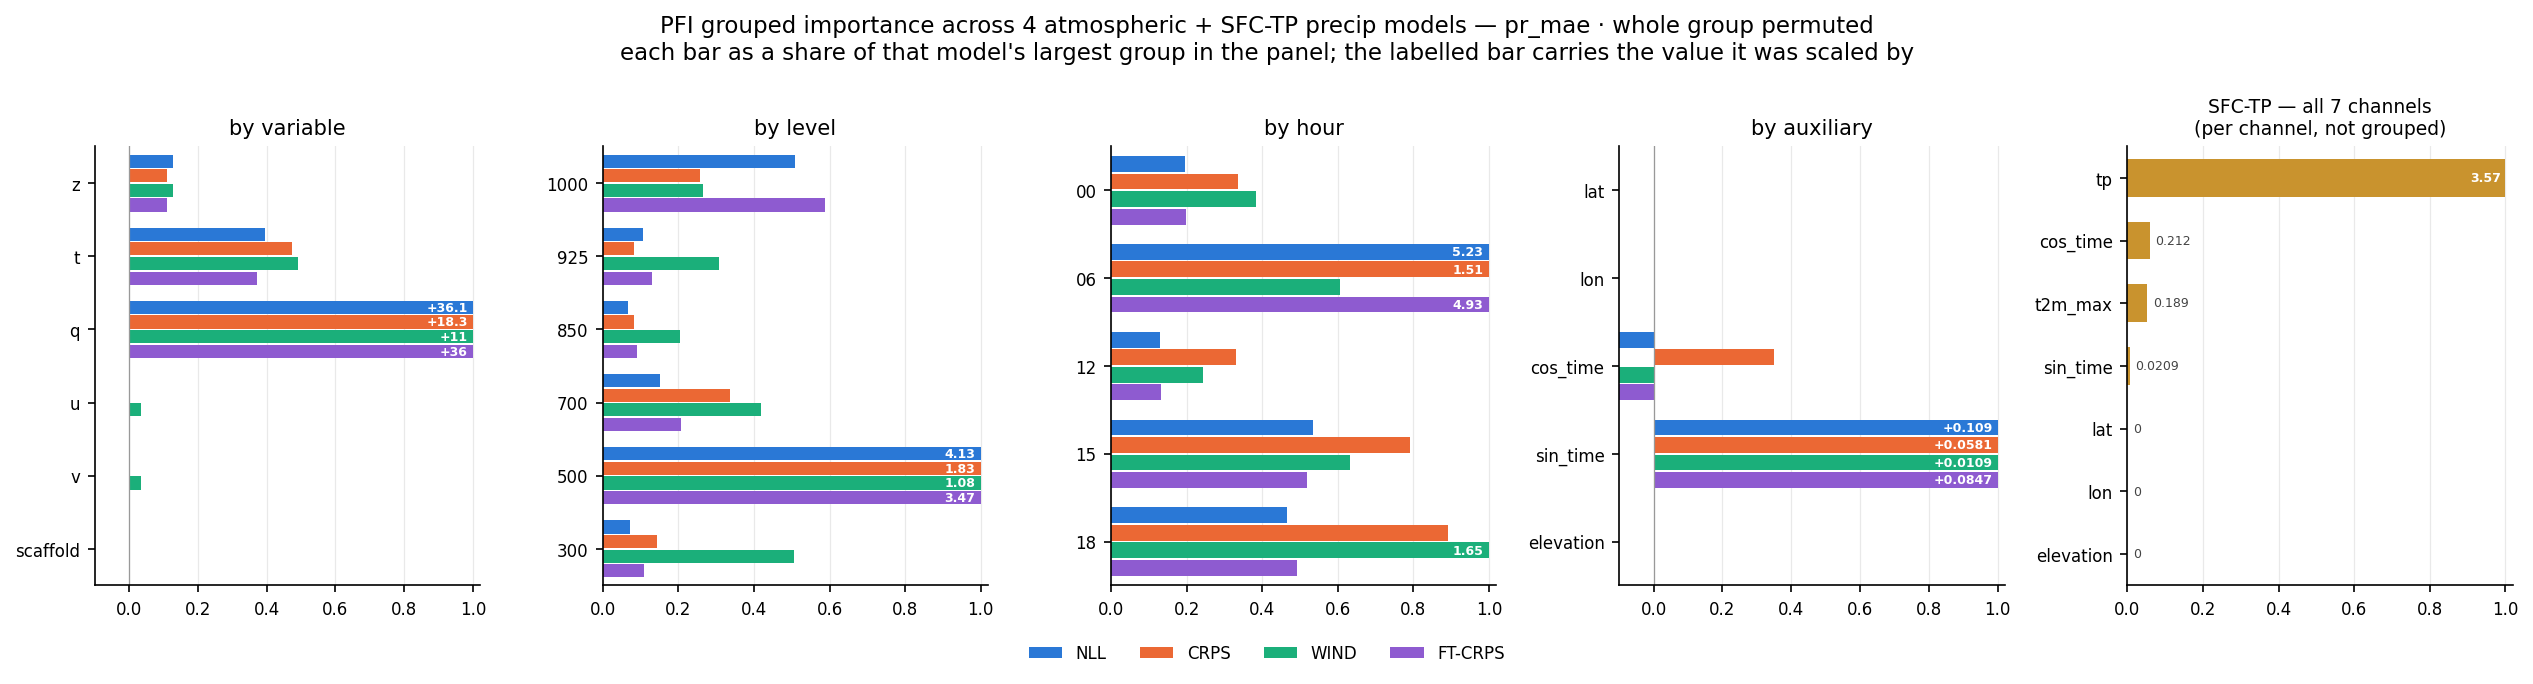
\includegraphics[width=\textwidth]{images/results/precip__fi_group_importance_pfi_2024__precip_processing_comparison__ALL.png}
\caption[Grouped permutation importance across the precipitation runs]{Grouped permutation
importance for the four atmospheric precipitation runs, on the 2024
holdout. Each model in the atmospheric runs is normalised by its peak contribution within each of the groups, to highlight relative importances. The normalisation constant is provided for each model in the full-length bar. \texttt{precip-SFC-TP} has no group permutation and is therefore represented independently. A bar
at or below zero means permuting that group changed the error by less than the noise of the estimate
itself, so it records no measurable contribution rather than a harmful one; the negative side of the
axis is cut short for that reason, and a bar reaching the cut is not a large negative.}
\label{fig:single-precip-fi}
\end{figure}


\subsection{Calibration}\label{subsec:single-precip-calibration}
Calibration is assessed with the probability integral transform of \fref{fig:single-precip-pit}, and
it enters the selection as a check rather than as a criterion.
\begin{figure}[H]
\centering
\subfloat[\texttt{precip-SFC-TP}]{%
  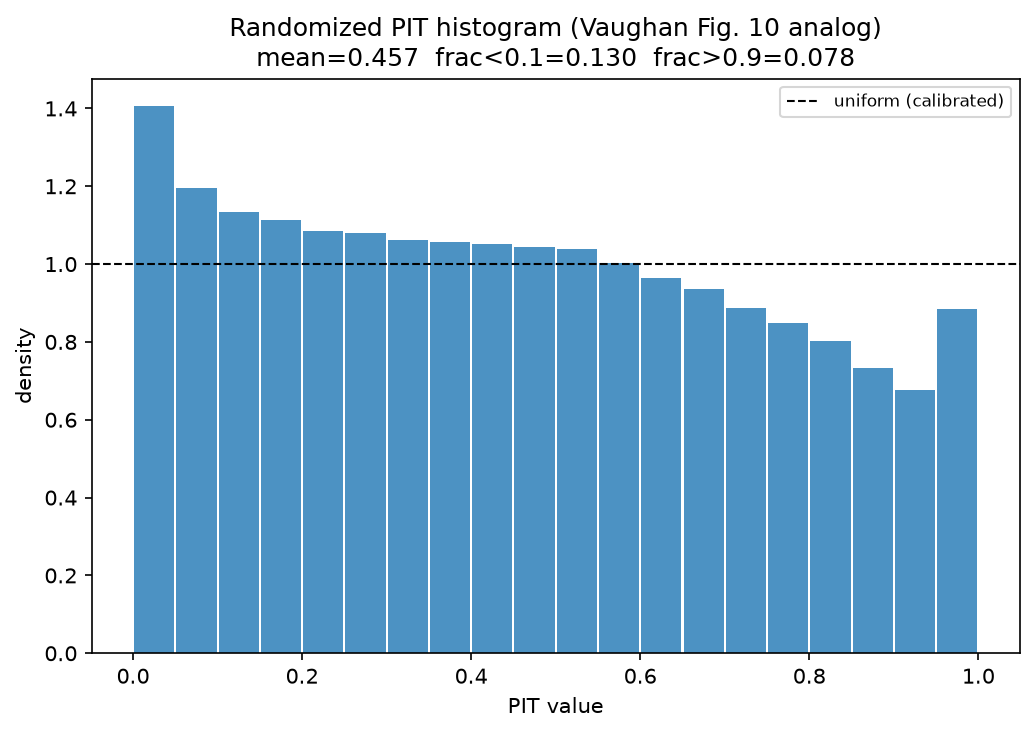
\includegraphics[width=0.49\textwidth]{images/results/precip__pit_histogram__eval_cv__clean_solo_precip_sfctp.png}}
\hfill
\subfloat[\texttt{precip-FT-CRPS}]{%
  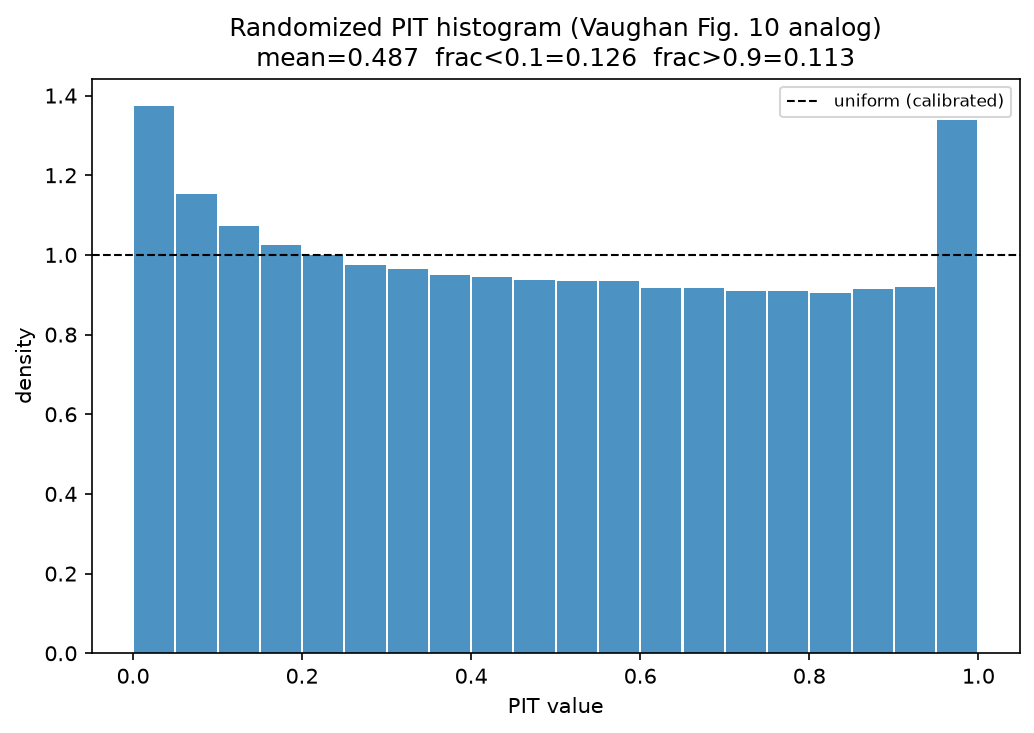
\includegraphics[width=0.49\textwidth]{images/results/precip__pit_histogram__eval_cv__clean_solo_precip_ftcrps.png}}
\caption[PIT histograms for the two selected runs]{Probability integral transform for the two
selected runs on the CV holdout, with the randomisation at the discrete point mass described in
\sref{subsec:app-skill-precip}. A calibrated forecast gives a flat histogram; a tilt towards low
values means too much probability is placed below the value that occurred.}
\label{fig:single-precip-pit}
\end{figure}

Every run places somewhat too much probability below the value that occurred. On the CV holdout the
PIT means of both selected models sit below the ideal $0.5$, \texttt{precip-FT-CRPS} at $0.487$ and
\texttt{precip-SFC-TP} at $0.457$. The PITs for the other models are reported in \tref{tab:single-precip-selection}.
\texttt{precip-SFC-TP} leans, carrying significant mass below $0.1$ and missing mass above 0.6,
whereas \texttt{precip-FT-CRPS} is nearly symmetric and departs from the ideal flat
 distribution as a shallow U rather than as a lean. Its leading PIT mean is therefore a near-balance of the two
ends rather than an absence of miscalibration.

The miscalibration is there in both models, but it is modest and of the same kind, a tilt of the
distribution rather than a collapse of the spread, and it points the same way for every run, so it
reorders none of the comparisons made above. Calibration enters the
model evaluation as a check  rather than a selection criterion and all models present acceptable calibration.

\FloatBarrier
\subsection{Model Selection}\label{subsec:single-precip-selection}

Unlike temperature (\sref{subsec:single-tmax-geography}), no single precipitation run leads on every
axis, so the choice here has to be argued rather than read off one figure.
\tref{tab:single-precip-selection} collects the evidence: the two skill scores against the bilinear
ERA5-Land reference, the Brier skill of \fref{fig:single-precip-categories} resolved
into its five intensity bands, the signed P98 tail bias and the PIT mean of
\sref{subsec:single-precip-calibration}, all on the CV holdout.

The aim in this work is to find a model that performs well and is robust. The winner is not clear. From feature importance \sref{subsec:single-precip-fi} we learn that the atmospheric models do appear to rely on the complexity of the diurnal cycle of the different input channels rather than overfitting on a single input channel. While the SFC model performs best in most
metrics, it fails in the extreme tail, where it is one of only two runs with a negative Brier skill
($-0.121$), and its lead rests almost entirely on the ERA5-Land total precipitation channel.
\texttt{precip-FT-CRPS} wins no column, but it is positive in all five bands, worst in none and the
closest to a uniform PIT. \texttt{precip-WIND} scores very similarly. However, as we saw for
temperature, its richer input probably needs a longer training budget to reach its potential.
\texttt{precip-NLL} and \texttt{precip-CRPS} fall off in performance: the first is worst in both heavy bands
and on the tail bias, the second is the weakest of the five in the three lightest bands, which hold nearly all of the
days.

We therefore keep two runs, one per input family. \texttt{precip-SFC-TP} is the choice wherever a
simple model is enough and the tail is not the target, \texttt{precip-FT-CRPS} the robust choice based on
atmospheric input.

\begin{table}[H]
\centering
\caption[Model-selection scorecard, all five precipitation runs]{The model-selection scorecard, on
the CV holdout. RPSS (\eref{eq:rpss}) and MAE skill (\eref{eq:mae-skill}) are both scored
against the shared bilinear ERA5-Land reference. The five BSS columns give the mean and standard
deviation, over the domain, of the per-point Brier skill of \fref{fig:single-precip-categories}, one column per intensity category.
The standard deviation is the spread across grid points, not an
uncertainty on the mean. P98 from \fref{fig:precip-indices},
positive meaning an overshot tail; PIT mean is from \sref{subsec:single-precip-calibration}, ideal
$0.5$. Green shades the best and red the worst run in each column, and the heavy rules pick out
\texttt{precip-FT-CRPS}, the atmospheric selected run. }
\label{tab:single-precip-selection}
\scriptsize
\setlength{\tabcolsep}{1.5pt}
\renewcommand{\arraystretch}{1.25}
\begin{tabular}{|>{\raggedright\arraybackslash}p{2.1cm}|>{\centering\arraybackslash}p{0.9cm}|>{\centering\arraybackslash}p{0.9cm}|>{\centering\arraybackslash}p{1.6cm}|>{\centering\arraybackslash}p{1.6cm}|>{\centering\arraybackslash}p{1.6cm}|>{\centering\arraybackslash}p{1.6cm}|>{\centering\arraybackslash}p{1.6cm}|>{\centering\arraybackslash}p{0.9cm}|>{\centering\arraybackslash}p{0.85cm}|}
\hline
\textbf{Run} & \textbf{RPSS} & \textbf{MAE} \newline \textbf{skill} &
\textbf{BSS dry} \newline \textbf{0--0.1} & \textbf{BSS weak} \newline \textbf{0.1--10} &
\textbf{BSS mod.} \newline \textbf{10--40} &
\textbf{BSS heavy} \newline \textbf{40--80} & \textbf{BSS extr.} \newline $\mathbf{\geq 80}$ &
\textbf{P98} \newline \textbf{(mm)} & \textbf{PIT} \newline \textbf{mean} \\
\hline
\texttt{precip-NLL} & $0.408$ & \cellcolor{red!12}$-0.234$ & $0.497 \pm 0.09$ & $0.453 \pm 0.09$ &
$0.198 \pm 0.14$ &
\cellcolor{red!12}$0.052 \pm 0.39$ & \cellcolor{red!12}$-0.350 \pm 0.91$ &
\cellcolor{red!12}$+11.15$ & $0.469$ \\
\hline
\texttt{precip-CRPS} & \cellcolor{red!12}$0.366$ & $-0.187$ & \cellcolor{red!12}$0.433 \pm 0.11$ &
\cellcolor{red!12}$0.415 \pm 0.10$ & \cellcolor{red!12}$0.195 \pm 0.14$ & $0.175 \pm 0.31$ & \cellcolor{green!12}$0.161 \pm 0.42$ &
$-5.71$ & \cellcolor{red!12}$0.418$ \\
\noalign{\hrule height 1.1pt}
\texttt{precip-FT-CRPS} & $0.416$ & $-0.145$ & $0.501 \pm 0.09$ & $0.454 \pm 0.09$ &
$0.209 \pm 0.14$ &
$0.140 \pm 0.32$ & $0.085 \pm 0.46$ & \cellcolor{green!12}$-0.68$ &
\cellcolor{green!12}$0.487$ \\
\noalign{\hrule height 1.1pt}
\texttt{precip-WIND} & $0.443$ & $-0.092$ & $0.518 \pm 0.08$ & $0.470 \pm 0.09$ &
$0.247 \pm 0.14$ &
$0.173 \pm 0.32$ & $0.086 \pm 0.70$ & $+2.16$ & $0.463$ \\
\hline
\texttt{precip-SFC-TP} & \cellcolor{green!12}$0.473$ & \cellcolor{green!12}$-0.032$ &
\cellcolor{green!12}$0.538 \pm 0.09$ & \cellcolor{green!12}$0.494 \pm 0.09$ &
\cellcolor{green!12}$0.288 \pm 0.13$ &
\cellcolor{green!12}$0.238 \pm 0.27$ & $-0.121 \pm 0.72$ & $+3.73$ & $0.457$ \\
\hline
\end{tabular}
\end{table}


Both selections hold up on the unseen year. The RPSS ordering of \fref{fig:single-precip-slope-skill}
is reproduced exactly in 2024, and both runs give up about $0.065$, as do the other three, so the loss
is shared rather than specific to either. Their MAE rises by $0.3$ and $0.45\,\mathrm{mm}$
(\fref{fig:single-precip-slope}), but the bilinear reference worsens by $0.28\,\mathrm{mm}$ in step,
so the distance to it barely moves and the MAE skill slips by only $0.01$ and $0.05$: 2024 is a
harder year rather than a year the models fail on. The indices of \fref{fig:precip-indices} agree,
both runs holding wet-day occurrence within a few percent of observed under either regime. 





\subsection{Discussion}\label{subsec:single-precip-discussion}



Two results of this section are worth separating from the model ranking. The first is that pointwise
error and distributional skill disagree in sign: no run beats bilinear interpolation in millimetres,
yet every run beats it by a wide margin on the five-category RPSS and on occurrence and intensity.
This is the behaviour the literature predicts. A smoothed coarse field is hard to beat on a squared
or absolute error while being wrong about the shape of the distribution, which is why the reference
calls wet days $38\,\%$ too often where the runs stay within a few per cent. The Bernoulli--Gamma
head is what buys that correction, as \textcite{cannon2008berngamma} report for density networks and
\textcite{vaughan2022convcnp} adopt for the same reason; the indices used here are theirs, and they
are used precisely because a pointwise score would hide the improvement. Their European,
station-based evaluation is not directly comparable to a Swiss gridded target, so no number is set
against theirs. The feature importance adds the interpretability side of the same point: the
atmospheric runs distribute their reliance across humidity, temperature and geopotential rather than
onto one channel, which is the meteorological rather than geographical reliance. \textcite{rampal2022interpretable} report the same for a grid-to-grid network over the New Zealand Southern Alps, read off saliency maps rather than permutation importance, so the conclusion now holds across two mountainous domains, two model geometries and two attribution methods.

The second is that the issue of extreme tail remains unsolved. The tail reversal of
\sref{subsec:single-precip-categories} is a CV-holdout result only: on 2024 the heaviest category is
negative for \emph{every} run, from \texttt{precip-SFC-TP} at $-0.05$ to \texttt{precip-NLL} at
$-0.21$, so \texttt{precip-CRPS}'s advantage there should not be carried over. A parametric
per-point head, whatever objective trains it, models each target point independently and has little
to work with where events are this rare. Generative and autoregressive approaches
\cite{harris2022generative, mardani2025corrdiff, bruinsma2023arcnp} address exactly this regime, at
the cost of the calibration that the present head gives directly.



\subsection{Conclusion}\label{subsec:single-precip-conclusion}

Two runs are carried forward: \texttt{precip-SFC-TP} where a simple surface model suffices, and
\texttt{precip-FT-CRPS} where robustness across the intensity range matters. Both correct the
occurrence and intensity errors of the coarse field, and both do so by a wide margin: their RPSS
against the bilinear ERA5-Land reference is $+0.47$ and $+0.42$ on the CV holdout and $+0.41$ and
$+0.35$ on the unseen year, a reduction of the ranked probability error of a third to a half in
either regime. Neither, however, improves on plain interpolation in millimetres. The heaviest rain remains the limit of what
this architecture and likelihood can deliver. 


% !TEX root = ../main.tex
% Chapter --- Verification at Independent Stations
\chapter{Verification at Independent Stations}\label{ch:stations}
In this chapter we compare selected results of  \cref{ch:single-model} to real measurements at weather stations. The target fields the model trained on are MeteoSwiss analyses, which are
themselves interpolated from station observations \cite{meteoswiss_ogd_grid} so the measurements are not completely independent. Three station sets
are used (\tref{tab:stations-sets}). All are MeteoSwiss open data, cover 2020--2024, and entered in this form no
training or model-selection step of this work: the homogenised daily temperature maxima of $28$ stations of the
Swiss National Basic Climatological Network (NBCN)~\cite{begert2005homogeneous,meteoswiss_ogd_nbcn},
the operational daily temperature maxima of $147$ SwissMetNet (SMN) stations, and the daily totals of $139$ SMN
rain gauges~\cite{meteoswiss_ogd_smn}.

\begin{table}[H]
\centering
\caption[Reference Meteorological Observations at Stations]{Three sets of observation station used for verification. A station enters its
set if it reports on at least $95\,\%$ of the days in 2020--2024; the day labelling of every series
was verified against its gridded counterpart before scoring (\sref{sec:app-stations}).}
\label{tab:stations-sets}
\footnotesize
\setlength{\tabcolsep}{4pt}
\begin{tabular}{|p{2.2cm}|p{1.5cm}|p{4.6cm}|p{2.2cm}|p{3.2cm}|}
\hline
\textbf{Set} & \textbf{Stations} & \textbf{Observable} & \textbf{Series} & \textbf{Verifies} \\
\hline
NBCN & $28$ & daily maximum $2\,\mathrm{m}$ temperature & homogenised & \texttt{atm+wind-clip60} \\
\hline
SMN temperature & $147$ & daily maximum $2\,\mathrm{m}$ temperature & operational & \texttt{atm+wind-clip60} \\
\hline
SMN rain gauges & $139$ & daily precipitation, $06$--$06\,\mathrm{UTC}$ & operational & \texttt{precip-FT-CRPS}, \texttt{precip-SFC-TP} \\
\hline
\end{tabular}
\end{table}

No regridding is involved in this comparison. The RBF final layer of \sref{subsec:meth-backbone}
decodes the predictive distribution at the station coordinates directly, so no gridded prediction is
resampled and no observation is interpolated. The gauge series is the $06$--$06\,\mathrm{UTC}$ daily
total, the accumulation window RhiresD itself uses \cite{meteoswiss_rhiresd_doc}. The reference at a
station is the same bilinear ERA5-Land interpolation as in \cref{ch:single-model}. 

\section{Temperature}\label{sec:stations-tmax}

\begin{figure}[H]
\centering
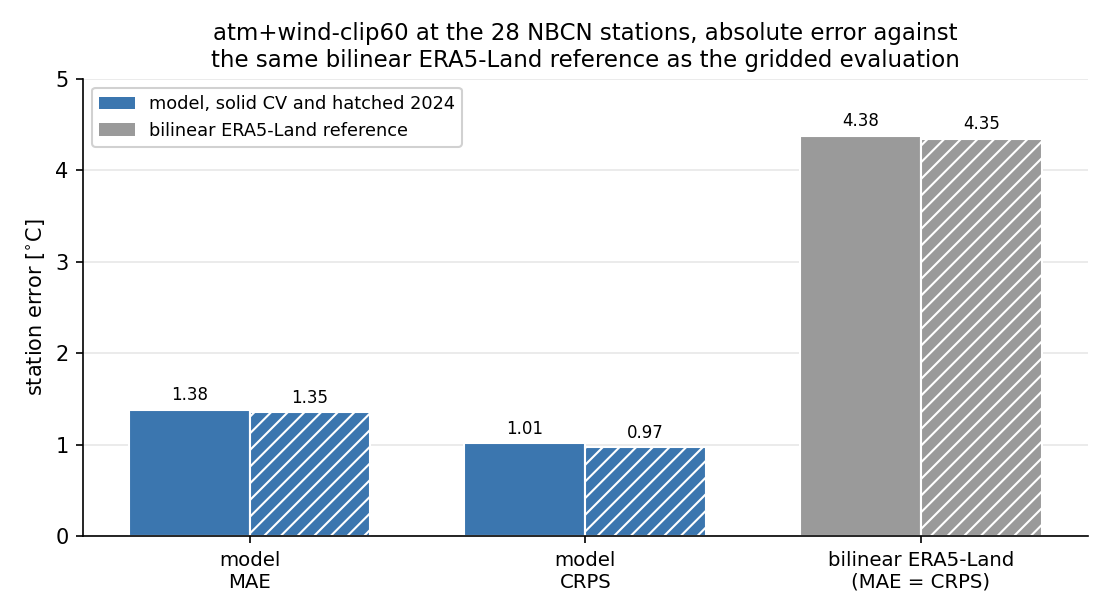
\includegraphics[width=\textwidth]{images/stations/tmax_selected_station_abs.png}
\caption[Verification at the 28 NBCN stations]{The selected temperature model at the $28$ NBCN
stations, solid bars for the CV holdout and hatched for 2024: the model's MAE and CRPS in physical
units, beside the bilinear ERA5-Land reference of \cref{ch:single-model}. The reference is
deterministic, so its CRPS equals its MAE and one bar serves both.}
\label{fig:stations-tmax-abs}
\end{figure}

The station comparison returns the verdict of \sref{subsec:single-tmax-geography}, and the
generalisation pattern of \fref{fig:single-tmax-slope} repeats at the measurement points:
\texttt{atm+wind-clip60} improves from $1.38$ to $1.35\,^{\circ}\mathrm{C}$ MAE between the CV
holdout and the unseen year (\fref{fig:stations-tmax-abs}). Station errors sit roughly
$0.3\,^{\circ}\mathrm{C}$ above their gridded counterparts throughout. In physical units the model reaches a station CRPS of $1.02$ and
$0.97\,^{\circ}\mathrm{C}$ against the $4.38$ and $4.35\,^{\circ}\mathrm{C}$ of the raw bilinear
reference, less than a quarter of the interpolation error in either regime. The pooled skill of
$0.77$ and $0.78$ is consistent with the gridded skill of $0.70$ and $0.71$ of \sref{subsec:single-tmax-unseen}\footnote{ \sref{subsec:single-tmax-unseen} already showed the
model scoring highest exactly where the reference fails, and at a station the reference is
handicapped further: it interpolates ERA5-Land to the station coordinates but not to the station
elevation, so at an alpine site much of its error is the unresolved elevation itself. The station
skill is therefore best read as confirmation of the gridded evaluation at real measurement points,
not as an absolute measure of the margin over interpolation.}.



\begin{figure}[H]
\centering
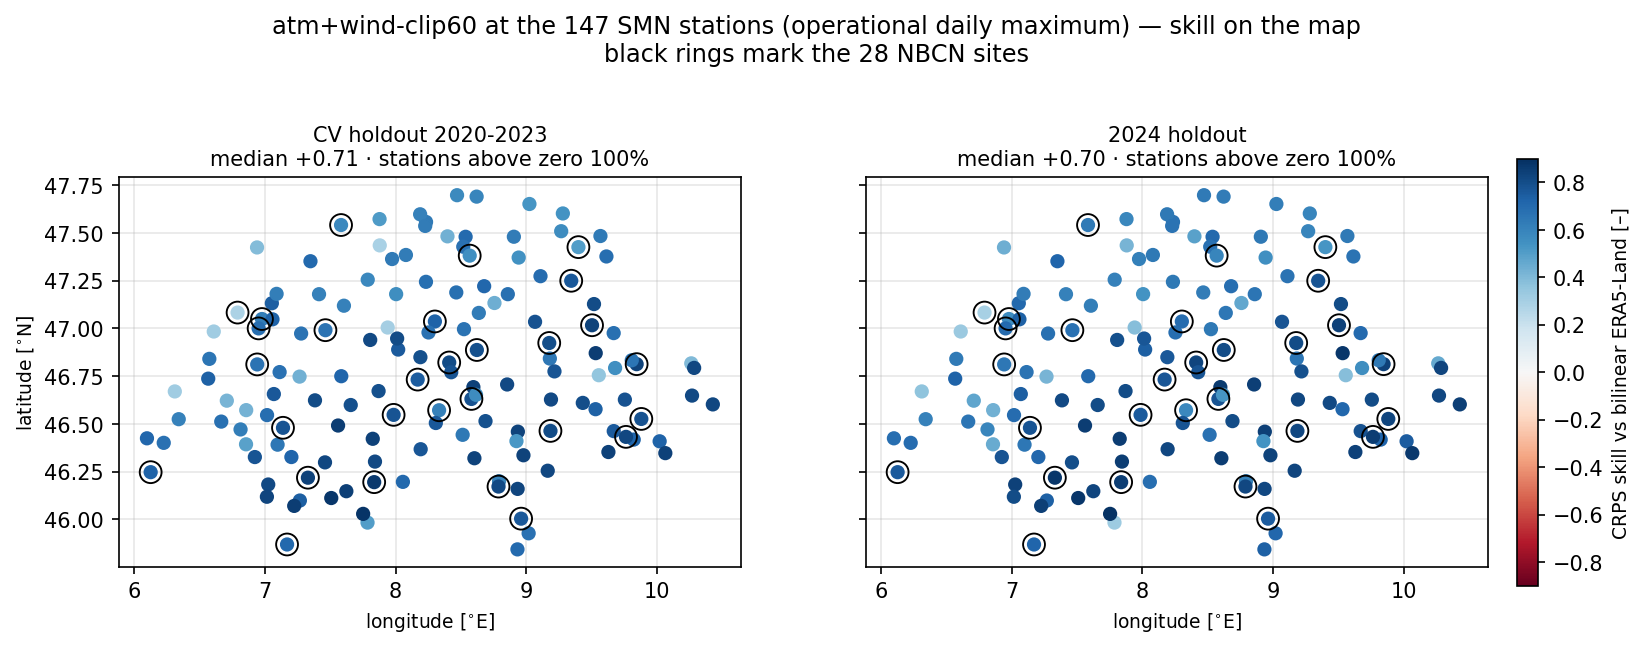
\includegraphics[width=\textwidth]{images/stations/tmax_station_skill_map_raw.png}
\caption[Skill at the 147 SMN stations]{Per-station CRPS skill of \texttt{atm+wind-clip60} against
the bilinear ERA5-Land reference at the $147$ SMN stations, under both regimes; black rings mark
the $28$ NBCN sites. The median station reads $+0.71$ and $+0.70$, and every station is above zero
in both regimes.}
\label{fig:stations-tmax-map}
\end{figure}

The claim survives breadth as well as quality. Widening the analysis from the $28$ homogenised NBCN
series to the $147$ SMN stations reporting the operational daily maximum confirms the model's superiority over interpolation: it reaches a station
MAE $1.41$ and $1.39\,^{\circ}\mathrm{C}$ across the two regimes, a median skill of $+0.71$ and
$+0.70$, and every station above zero (\fref{fig:stations-tmax-map}). At the
$28$ sites the two cohorts share, the operational and homogenised series give per-station errors
that agree to a median of $0.00\,^{\circ}\mathrm{C}$ over this span, so the distinction between the
two series carries no weight here. The model therefore beats interpolation at every real
measurement point it was tested on. 

\section{Precipitation}\label{sec:stations-precip}

For precipitation this comparison
sharpens the conclusions of \sref{sec:single-precipitation}. The
occurrence prediction of the bilinear ERA5-Land fails: it identifies half of all days as
wet ($0.50$ against an observed frequency of $0.33$ on the CV holdout), while both selected runs
stay within $0.05$ of the observed frequency in both regimes. This is the station-level counterpart
of the R01 result of \fref{fig:precip-indices}.

\begin{figure}[H]
\centering
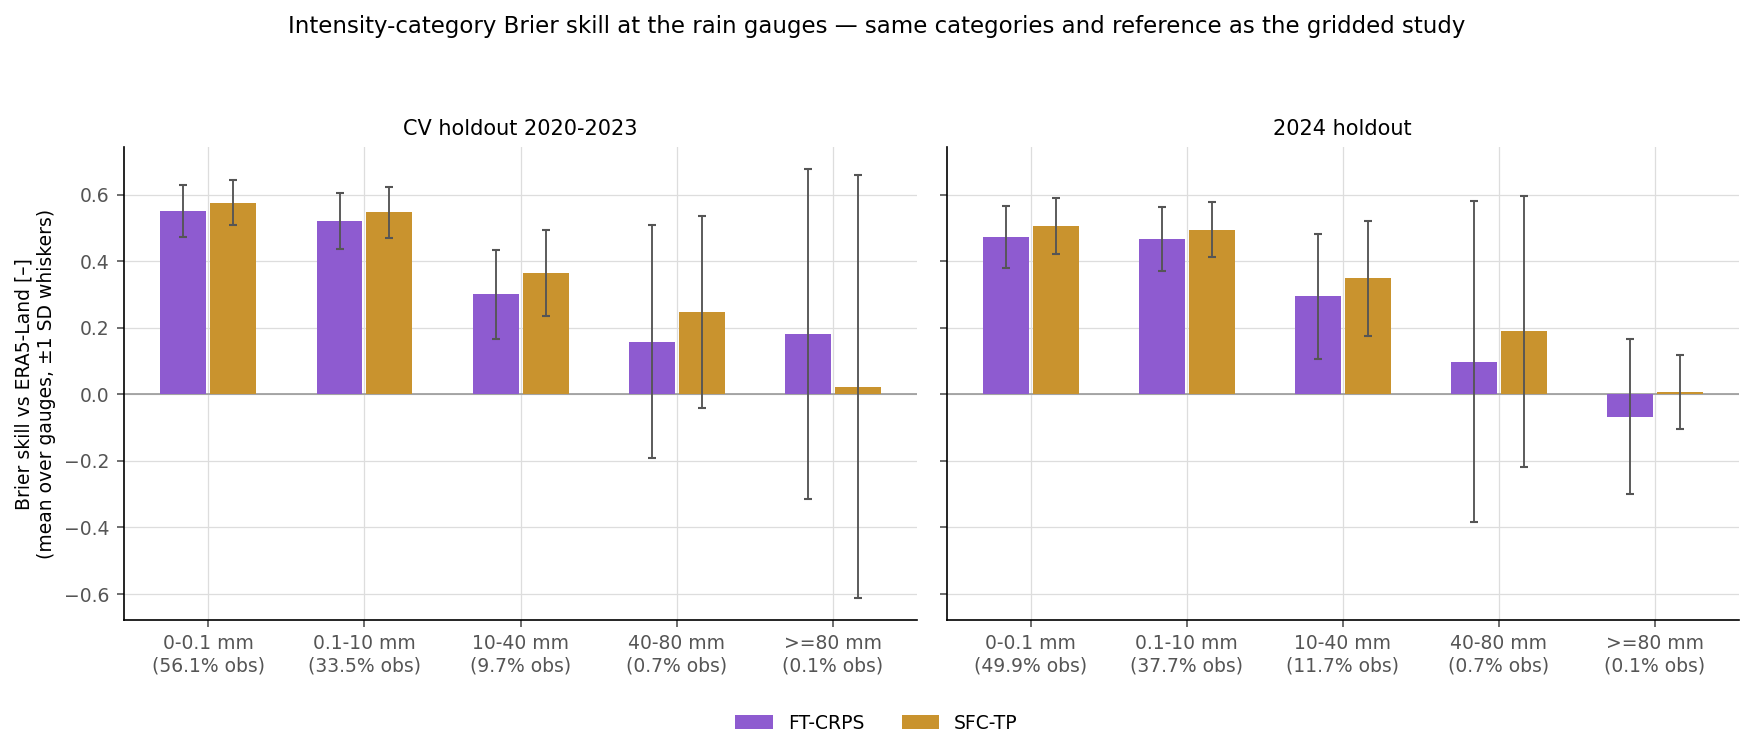
\includegraphics[width=\textwidth]{images/stations/precip_category_bss.png}
\caption[Intensity-category Brier skill at the rain gauges]{Brier skill against the bilinear
ERA5-Land reference at the $139$ gauges, by intensity category, the same categories and reference
construction as \fref{fig:single-precip-categories}. For each category, the bar shows the mean of
the per-gauge Brier skills and the whisker their $\pm 1$ standard deviation across gauges, a spread
rather than a standard error; the observed frequency of the category is noted beneath it.}
\label{fig:stations-precip-bss}
\end{figure}

Scored by intensity category, the gauges reproduce the gridded structure of
\sref{subsec:single-precip-categories} (\fref{fig:stations-precip-bss}). Skill falls
with intensity for both runs, and \texttt{precip-SFC-TP} leads in every category that carries an
appreciable share of days, exactly as in the gridded ordering. The mean skill stays positive
through the $40$--$80\,\mathrm{mm}$ category ($+0.25$ and $+0.19$ for \texttt{precip-SFC-TP},
$+0.16$ and $+0.10$ for \texttt{precip-FT-CRPS}, across the two regimes) and is indistinguishable
from zero at $\geq 80\,\mathrm{mm}$, where the whiskers span both signs. The heaviest events remain
the limit of what these models deliver, at the gauges as on the grid.

The surface-based run is ahead of the free-troposphere run at every category below $80\,\mathrm{mm}$, in both regimes. The advantage is small but consistent. However as the gridded evaluation is not independent of the station verification, this does not contradict the conclusion of \sref{sec:single-precipitation}. The station verification is a confirmation of the gridded evaluation, not an independent assessment of the two runs against each other. 

\begin{figure}[H]
\centering
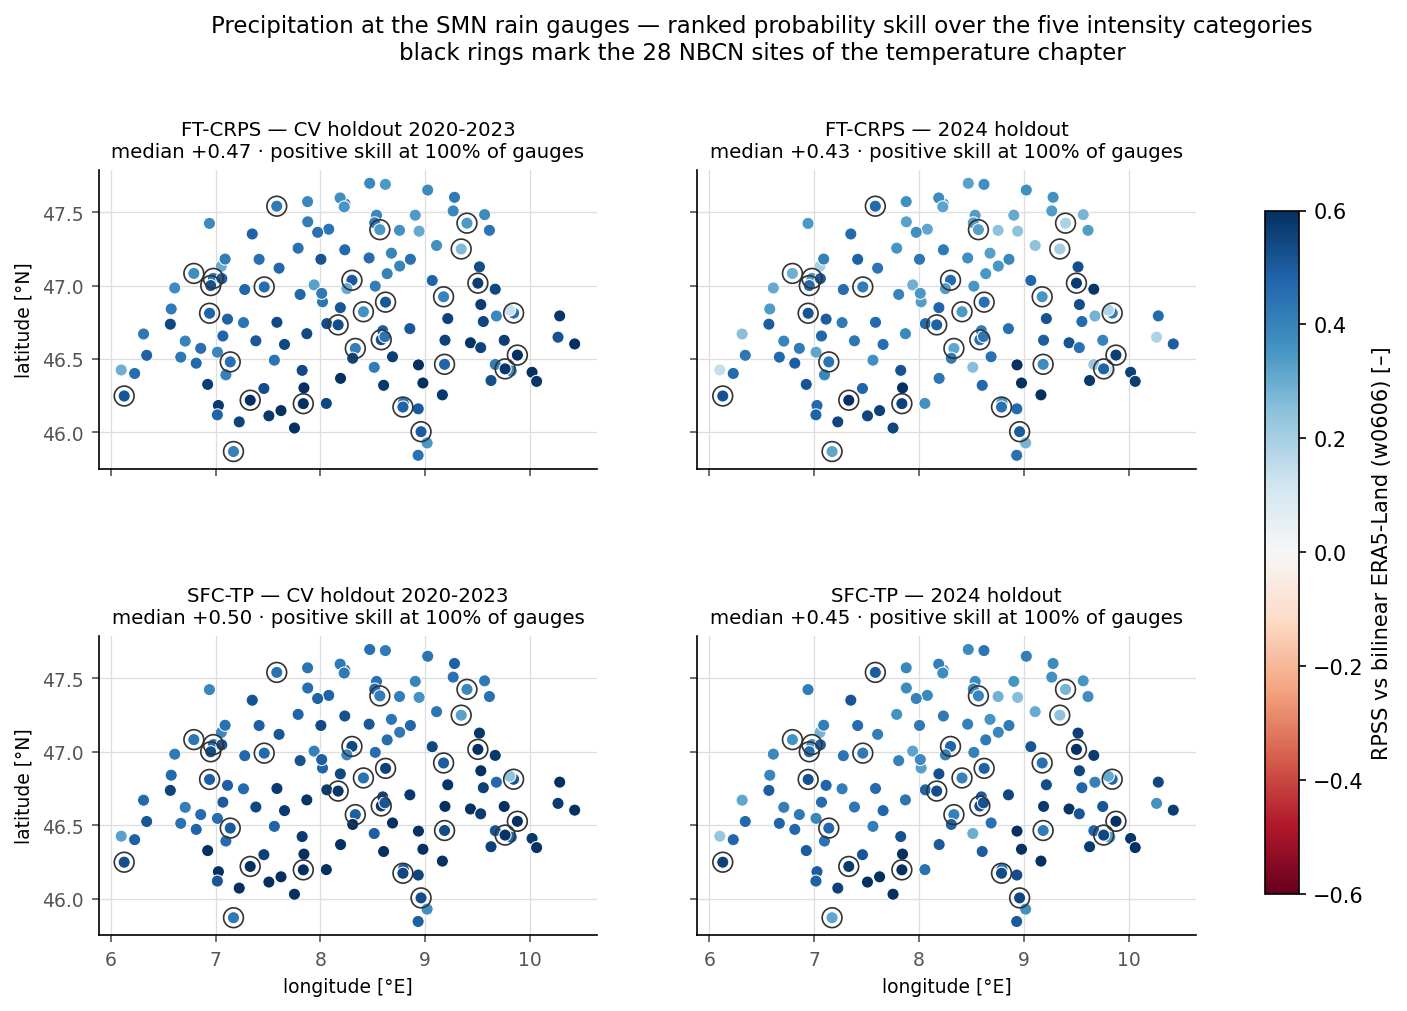
\includegraphics[width=\textwidth]{images/stations/precip_gauge_skill_map.png}
\caption[Ranked probability skill at the 139 rain gauges]{Per-gauge ranked probability skill over
the five intensity categories, against the bilinear ERA5-Land reference, for both selected runs and
both regimes; black rings mark the $28$ NBCN sites.}
\label{fig:stations-precip-map}
\end{figure}


Pooled over the categories, both runs beat plain interpolation at every one of the $139$ gauges, in
both regimes: the median ranked probability skill is $+0.50$ and $+0.45$ for
\texttt{precip-SFC-TP} and $+0.47$ and $+0.43$ for \texttt{precip-FT-CRPS}
(\fref{fig:stations-precip-map}). 

\begin{figure}[H]
\centering
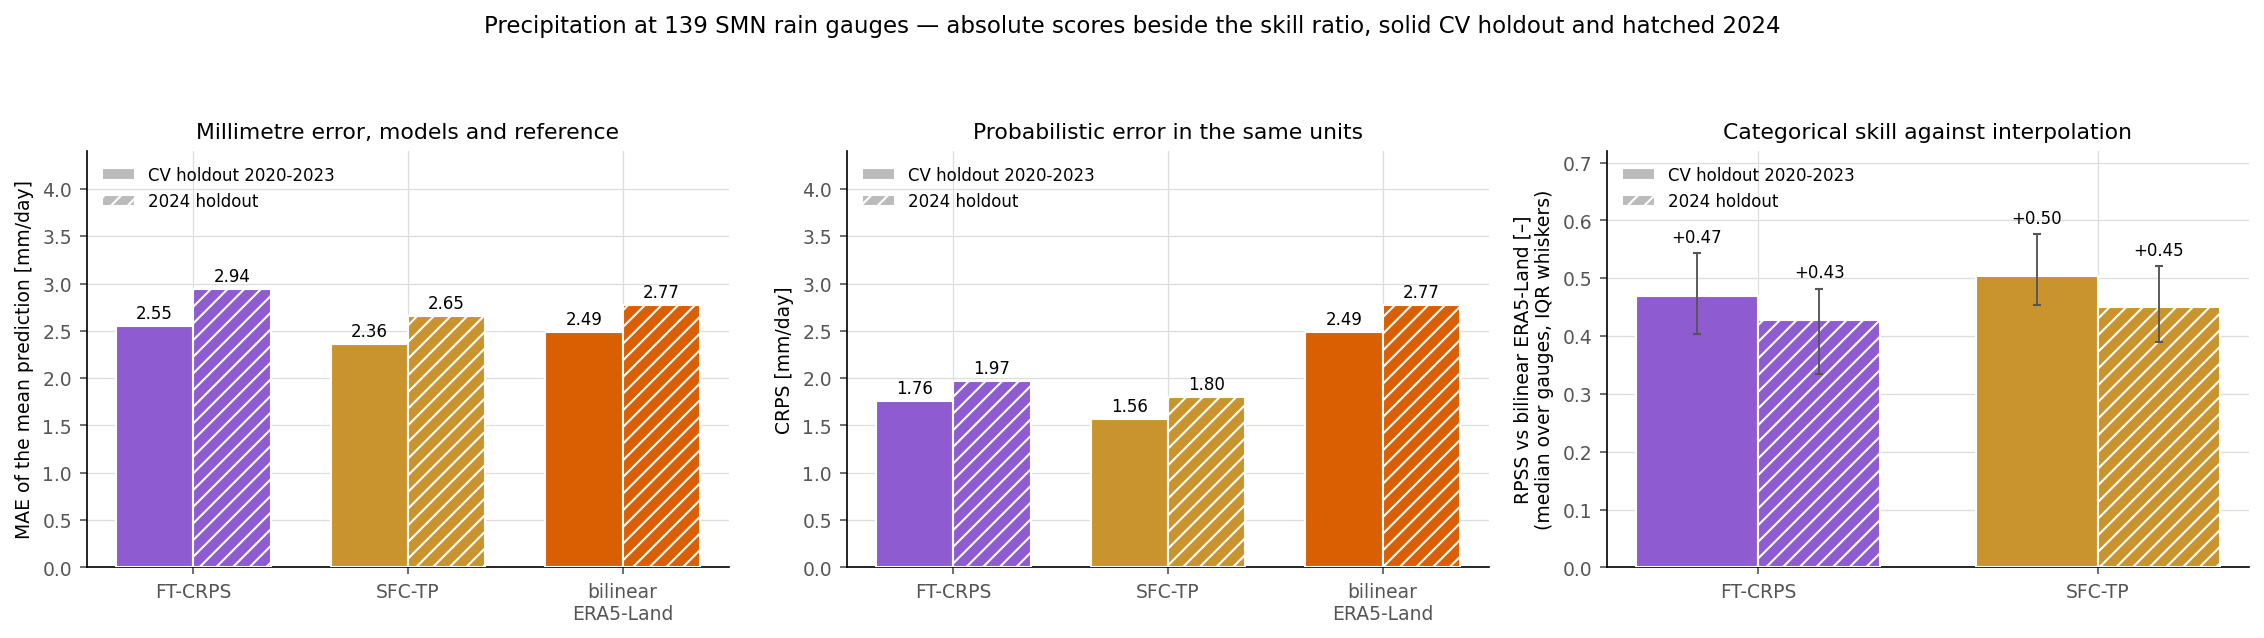
\includegraphics[width=\textwidth]{images/stations/precip_absolute_values.png}
\caption[Absolute scores at the rain gauges]{The two selected precipitation runs at the $139$
gauges, solid bars for the CV holdout and hatched for 2024. Left: MAE of the mean of the predicted
distribution. Middle: CRPS of the full distribution, in the same units; the reference carries no
distribution, so its CRPS is its MAE and the same bar serves both panels. Right: the median
per-gauge ranked probability skill, with interquartile whiskers.}
\label{fig:stations-precip-abs}
\end{figure}

\fref{fig:stations-precip-abs} restates the gauge verification in absolute units, since a ranked
probability skill of $+0.50$ says nothing about the size of the errors underneath it. The millimetre
picture remains a near-tie, with one shift of sign against \fref{fig:single-precip-slope-skill}:
scored as a point forecast through the mean of its predicted distribution, \texttt{precip-SFC-TP} performs ahead of the reference ($2.36$ and $2.65\,\mathrm{mm\,day^{-1}}$ against $2.49$ and
$2.77$ across the two regimes; the reference is scored at the gauges here, so these are not the
$2.29\,\mathrm{mm}$ it reaches on the gridded target), where on the grid it was marginally behind, while
\texttt{precip-FT-CRPS} stays behind at $2.55$ and $2.94$. A plausible reason is the target itself:
the gridded truth is an interpolated, smoothed field, which flatters a smooth reference in a
pointwise score, whereas a real gauge series is rougher and penalises it. Scored as distributions, both runs are clearly ahead, at a CRPS of
$1.56$ and $1.80\,\mathrm{mm\,day^{-1}}$ for \texttt{precip-SFC-TP} and $1.76$ and $1.97$ for
\texttt{precip-FT-CRPS}, between $29$ and $37\,\%$ below the reference in every case. The whole
panel shifts upward from the CV holdout to 2024, the reference included, so the deterioration on the
unseen year belongs at least partly to the year rather than to the models.

% !TEX root = ../main.tex
% Chapter --- Conclusion
\chapter{Conclusion}\label{ch:conclusion}

\section{Findings}\label{sec:concl-findings}

This work trained convolutional conditional neural processes to downscale ERA5 and ERA5-Land to the
$1\,\mathrm{km}$ MeteoSwiss grid, for daily maximum temperature with a Gaussian head and for daily
precipitation with a Bernoulli--Gamma head, and evaluated them across input sets, objectives and
two strictly separated evaluation regimes: cross-validated holdout over 2020--2023 and an unseen
2024. The Alps are a demanding place to do this, because the terrain that decides the local weather
is exactly the terrain the coarse fields average away. This section summarises the findings and
evaluates them against the research questions posed in \sref{sec:intro-questions}.

For temperature we determined a clear  improvement when choosing atmospheric over the surface input. It beats surface
input on every accuracy measure, MAE, RMSE, CRPS and skill, in both evaluation regimes, and the two input
families do not merely differ in accuracy but also in how they generalise. Every atmospheric
configuration holds or improves its score on the unseen year, while both surface
configurations degrade. The gap between them opens primarily in the cold season, when the
fine-scale truth decouples from the coarse surface field and only the atmospheric context can
correct for this offset. This is the regime in which a purely spatial mapping is expected to fail,
and the feature-importance study shows why one works while the other fails. The atmospheric models lean on lower-tropospheric
temperature at physically sensible levels and hours rather than on coordinate, season or terrain
channels, so what has been learnt is a meteorological relationship and not a trained spatial
interpolation. \textcite{rampal2022interpretable} reach the same verdict for rainfall over the
New Zealand Southern Alps with a grid-to-grid network and saliency maps, so the finding is not
particular to this architecture or to this mountain range. The result is well calibrated and predicts cautiously on data it has never seen, which is the behaviour a user would want.


Precipitation behaves differently. The atmospheric runs spread their reliance across humidity,
temperature and geopotential, which is again the meteorologically meaningful behaviour, yet a
surface run driven by the coarse precipitation field matches or beats them on most pooled scores.
The atmospheric run fine-tuned on the CRPS is ahead of the surface run in the heaviest intensity
category on the cross-validated holdout, but that advantage does not survive the unseen year, where
every run scores at or below zero. Calibration for both configurations is acceptable.

Both atmospheric and surface input are viable for precipitation. However the reliance of a sole input channel of the surface configuration carries the risk of overfitting and missing meteorological relationships. As performance is similar, the atmospheric input is preferred for its more robust generalisation and meteorological interpretability.


Due to its available input resolution, the atmospheric input is not more expensive than surface runs. The bottleneck of the architecture is the distance matrix that maps from the input grid to the target points.
Therefore the significantly larger number of input channels, $95$ against at most $7$ in the
surface configurations, is more than paid for by the coarser $0.25^{\circ}$ lattice they are
carried on. Training peaks
below $2.2\,\mathrm{GB}$ at the batch size of $8$ used here and inference roughly halves that, so a single
mid-range GPU is sufficient for training and inference.

In complex terrain the architecture holds up for both variables. The selected temperature model
reaches a skill of $0.71$ over bilinear ERA5-Land and an MAE of $1.03\,^{\circ}\mathrm{C}$ on the
unseen year. It is skilful at all of the $147$ SMN stations, with a median skill of $+0.71$ (CV) and
$+0.70$ (unseen). It has to be stated that those stations feed the gridded analyses the model was
trained on and are therefore not a fully independent check (\cref{ch:stations}).
\textcite{vaughan2022convcnp} report an MAE of $1.19\,^{\circ}\mathrm{C}$ at stations their model
never saw, against $1.35\,^{\circ}\mathrm{C}$ for their Gaussian-process baseline, and name Alpine
terrain as the region where their largest errors concentrate, without quantifying it separately. A
continent-wide station mean is no benchmark for a domain that is Alpine throughout, and the target
here is a gridded analysis rather than a station series, so the two numbers are context rather than
a head-to-head comparison. What this work adds is a measurement of exactly that region.

For precipitation the answer depends on what is being asked. Distributionally the models beat
interpolation by a wide margin: the ranked probability skill of the two selected runs is $+0.47$ for \texttt{precip-SFC-TP} and
$+0.42$ for \texttt{precip-FT-CRPS} on the cross-validated holdout and $+0.41$ and $+0.35$ on the unseen year.
At the $139$ rain gauges the lowest median skill is $+0.43$.
Evaluated on the predicted accumulation in millimetres, no run beats
the ERA5 reference on the gridded target. One run reverses that verdict at the gauges:
\texttt{precip-SFC-TP} beats the reference there in both regimes, by $0.13$ and
$0.12\,\mathrm{mm\,day^{-1}}$, as expected when a smoothed reference is scored against a smoothed,
interpolated truth.

One known weakness of statistical downscaling is the drizzle bias of the coarse field, which calls wet days $38\,\%$ too often. The Bernoulli--Gamma head removes that bias and restores the observed intensity along with it. 

On the precip models we showed that objective can impact the extreme tail. This lever however is not sufficient to close the gap, and a dedicated treatment of the tail is needed if accuracy in this region is required. The temperature models also present a tendency to over-predict temperature above $30\,^{\circ}\mathrm{C}$.



\section{Limitations and Future Work}\label{sec:concl-future}

The limitations below bound what the results above can claim, and point to directions for future work.

\begin{itemize}
\item \textbf{No spatial coherence.} The factorised head predicts one marginal per target point
(\sref{sec:bg-neural-processes}, \sref{subsec:meth-gaussian}), so every score is marginal, no
multi-point product such as a catchment mean is available, and spatial oversmoothing cannot be
judged at all. Autoregressive sampling of the existing checkpoints~\cite{bruinsma2023arcnp} would
settle it without retraining; a joint Gaussian head~\cite{andersson2023convgnp} is the fuller fix.

\item \textbf{The extreme tail.} No objective and no input reached it, for either variable, and
temperature has no tail-specific score at all. It needs a dedicated treatment, upper-tail
post-processing or a generative refinement step~\cite{harris2022generative, mardani2025corrdiff}.

\item \textbf{Four years, and a schedule still improving.} Doubling the epoch budget beat every
input modification tested (\sref{subsec:single-tmax-discussion}), so a longer training schedule, and a training period extended over more years to cover more rare events, is the natural next step. The same holds for the evaluation: 2024 is a single year, so the conclusions drawn from it may be shaped by the particular events it contained. A longer training period and more holdout years would provide a more robust evaluation of the model's performance.

\item \textbf{Computation spent where it is not scored.} The loss is formed inside the Swiss border
only, so $47\,\%$ of the RBF and elevation-MLP work carries no gradient. Supervising the whole target set would improve border accuracy. The width of the elevation MLP is the other open cost question: cost argues for a narrower
one, the seasonal-input result for a wider one, and neither was tested.

\item \textbf{Independence of station data.} The gridded target is interpolated from the same station network the verification uses, so the two are not fully independent. A stronger test would verify against an independently constructed product.
\item \textbf{Is the learnt relationship physically meaningful?} The feature-importance study shows reliance on physically sensible inputs, which is evidence, not proof. Applying the trained model to comparable terrain elsewhere in the Alpine range would test whether the relationship travels, and the architecture permits it without retraining: the trunk is convolutional, the target set is arbitrary, and the elevation features are physical quantities computable from any terrain model. Only the coordinate channels are anchored to the training domain, and the near-zero reliance on them is exactly what such a transfer would confirm or refute; a retraining without latitude and longitude as inputs would remove that anchor altogether and show directly how much the model needs them.
\item \textbf{Is the model robust to climate change?} The training years are historical, so nothing here shows whether the learnt mapping holds in a warmer climate; scenario-driven input would test that.
\item \textbf{Weather models over reanalysis.} The input is reanalysis. Driving the same model with forecast fields, which carry different biases, would show whether the downscaling survives them, and would open the route to real-time use.
\item \textbf{The fold ensemble against a single model.} Inference uses the five cross-validation fold models as an ensemble rather than a model retrained on the full 2020--2023 span (\sref{subsec:meth-cv}); this was not compared against, so it is untested whether the ensemble is actually more accurate. A model trained on the full span would add a clean baseline to check that against, and access to all five blocks of training data at once, rather than the four out of five each fold model sees.
\end{itemize}

%%%%%%%%%%%%%%%%%%%%%%%%%%%%%%%%%%%%%%%%%%%%%%%%%%%%%%%%%%%%%%%%%%%%%%%%%%%%%%%%%%%%%%%%%%
%\nocite{*}
\printbibliography[notkeyword=data, title=References,   heading=bibintoc]
\printbibliography[keyword=data,    title=Data Sources, heading=bibintoc]
%%%%%%%%%%%%%%%%%%%%%%%%%%%%%%%%%%%%%%%%%%%%%%%%%%%%%%%%%%%%%%%%%%%%%%%%%%%%%%%%%%%%%%%%%%

% !TEX root = ../main.tex
% Appendix
\appendix
\chapter{Appendix}\label{ch:appendix}

\section{Preprocessing Details}\label{sec:app-preprocessing}

\sref{subsec:data-coords} summarises the preprocessing pipeline; the full step-by-step procedure,
each step depending on the ones before it, is given here.

\begin{enumerate}
    \item \textbf{Reference frames} ERA5 and ERA5-Land use a regular latitude--longitude grid in WGS84; the MeteoSwiss grids and the DHM25 topography use the projected Swiss LV95 system, whose axes are in metres.
    \item \textbf{Encoder grid}\label{item:data-encoder-grid} Which lattice carries the input channels depends on the configuration. The surface configurations use the ERA5-Land $0.1^{\circ}$ grid as it comes. The atmospheric configurations use the ERA5 $0.25^{\circ}$ pressure-level grid in its native resolution, and the whole scaffold, the two coordinate channels, the seasonal pair and the coarse elevation, is rebuilt on that same coarse lattice so that every channel of a configuration shares one geometry. The alternative, kept for comparability with the surface runs, bilinearly interpolates the $0.25^{\circ}$ fields onto the $0.1^{\circ}$ surface grid.
    \item \textbf{Target locations}\label{item:data-target-locations} The MeteoSwiss target coordinates are taken from the WGS84 fields that ship with the product and are min--max normalised to $[0,1]$ against the ERA5-Land bounding box, the atmospheric configurations inheriting that same box so the normalisation is identical everywhere. It is a storage convention only: the distance matrix de-normalises them back to degrees, and the topography lookup reprojects the original WGS84 degrees to LV95 metres.
    \item \textbf{Topography lookup} For the topographic features, the target coordinates are transformed to LV95 and the DHM25 fields are bilinearly interpolated at each target point (\sref{sec:data-topography}). These three features reach the elevation MLP in raw metres; they are not normalised.
    \item \textbf{Grid geometry}\label{item:data-grid-geometry} The squared distance between every target point and every point of the encoder grid of step~\ref{item:data-encoder-grid} is computed once, in degrees, and reused in every forward pass, where the final layer turns it into the interpolation kernel (\sref{subsec:meth-backbone}). The target coordinates are converted back from the normalised form of step~\ref{item:data-target-locations} to degrees for this, and the matrix is built against the coarse lattice in the native-grid configurations. A degree of longitude counts the same as a degree of latitude here.
    \item \textbf{Time frames} The pressure-level channels are instantaneous fields at $00$, $06$, $12$, $15$ and $18\,\mathrm{UTC}$, and the two surface anchors are sampled at the same hours but are not the same kind of field: $\mathrm{t2m}$ is the instantaneous $2\,\mathrm{m}$ temperature at each hour, while $\mathrm{tp}$ is the hourly accumulation ending at the snapshot time. The daily ERA5-Land fields for surface configurations cover the UTC calendar day: the daily maximum for temperature, and for precipitation the daily total, recovered from the hourly accumulation that ERA5-Land resets at $00\,\mathrm{UTC}$.
     \newline The precipitation target instead runs from $06\,\mathrm{UTC}$ to $06\,\mathrm{UTC}$ of the following day (\sref{sec:data-targets}) resulting in a six-hour offset. \newline Input and target are matched by date only and no shift is applied. When ERA5-Land field is used as reference forecast of the precipitation skill scores it is reprocessed using the hourly accumulation to match the target $06\,\mathrm{UTC}$ to $06\,\mathrm{UTC}$ evaluation.
    \item \textbf{Temperature targets} The MeteoSwiss temperature is converted from degrees Celsius to Kelvin and then $z$-scored with the mean and standard deviation of the ERA5-Land $\mathrm{t2m\_max}$ field. This ensures input and target share a normalisation.
    \item \textbf{Precipitation targets} Precipitation is kept in raw millimetres. A $z$-score would shift the many exact zeros to negative values and break the Gamma log-likelihood of the Bernoulli--Gamma head (\sref{subsec:meth-likelihoods}); the dry days have to stay exactly zero.
    \item \textbf{Input channels} The channels are normalised according to their type:
    \begin{itemize}
        \item \emph{Meteorological fields.} Every field channel is $z$-scored with its own mean and standard deviation: the pressure-level fields, where each combination of variable, level and hour forms its own channel, the surface temperature, and the surface anchors.\footnote{The limitation in normalisation of the precipitation target does not apply to the precipitation input channel, which is normalised with its own statistics, as it has no requirements from a proposed distribution.}
        \item \emph{Coordinate channels.} Latitude and longitude are min--max normalised to $[0,1]$ with the bounds of the ERA5 input grid, the same bounds used for the target locations.
        \item \emph{Seasonal channels.} The day of year is encoded as the pair $\bigl(\cos(2\pi\,(d-1)/365), \sin(2\pi\,(d-1)/365)\bigr)$, where $d$ is the day of the year from 1 to 366; both components are bounded by construction and are used as they are. Therefore, they are not normalised by design.
        \item \emph{Elevation channel.} The static geopotential is divided by the standard gravity $g = 9.80665\,\mathrm{m/s^{2}}$ before use, so this channel holds the model orography as a height in metres and not a geopotential, and is $z$-scored with its own statistics on the grid it is built on. The pressure-level geopotential is \emph{not} converted: it enters as it comes and is $z$-scored like the other meteorological fields.
    \end{itemize}
    \item \textbf{Persistence} All normalisation statistics, the ordered channel names and the grid coordinates are stored with the trained model, so evaluation and inference normalise new data with exactly the statistics seen during training.
\end{enumerate}

\FloatBarrier
\section{Output Distributions}\label{sec:app-distributions}

\fref{fig:meth-tmax-dist} and \fref{fig:meth-precip-dials} illustrate the two predictive
distributions of \sref{sec:meth-distributions} at a single target point and day.

\begin{figure}[H]
\centering
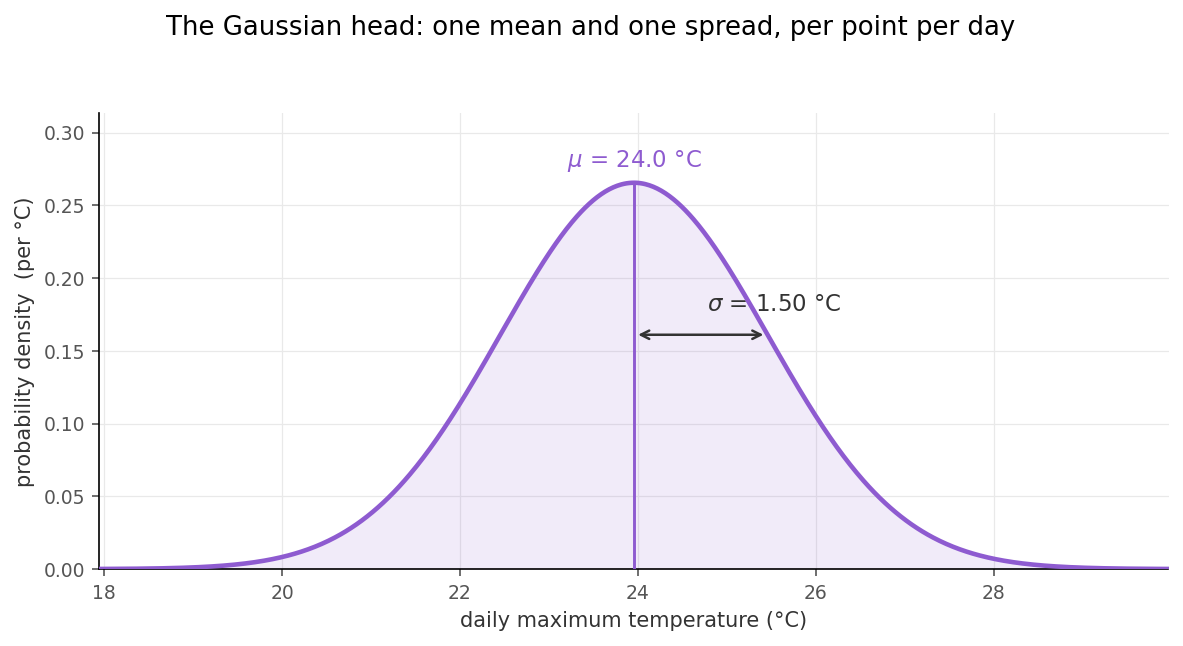
\includegraphics[width=0.9\textwidth]{images/16_tmax_distribution.png}
\caption[The Gaussian predictive distribution]{The Gaussian predictive density for a single target point and day. The model outputs the two parameters: the mean $\mu$ locates the distribution and the standard deviation $\sigma$ sets its width, shown here for $\mu = 24.0\,^{\circ}\mathrm{C}$ and $\sigma = 1.5\,^{\circ}\mathrm{C}$.}
\label{fig:meth-tmax-dist}
\end{figure}

\begin{figure}[H]
\centering
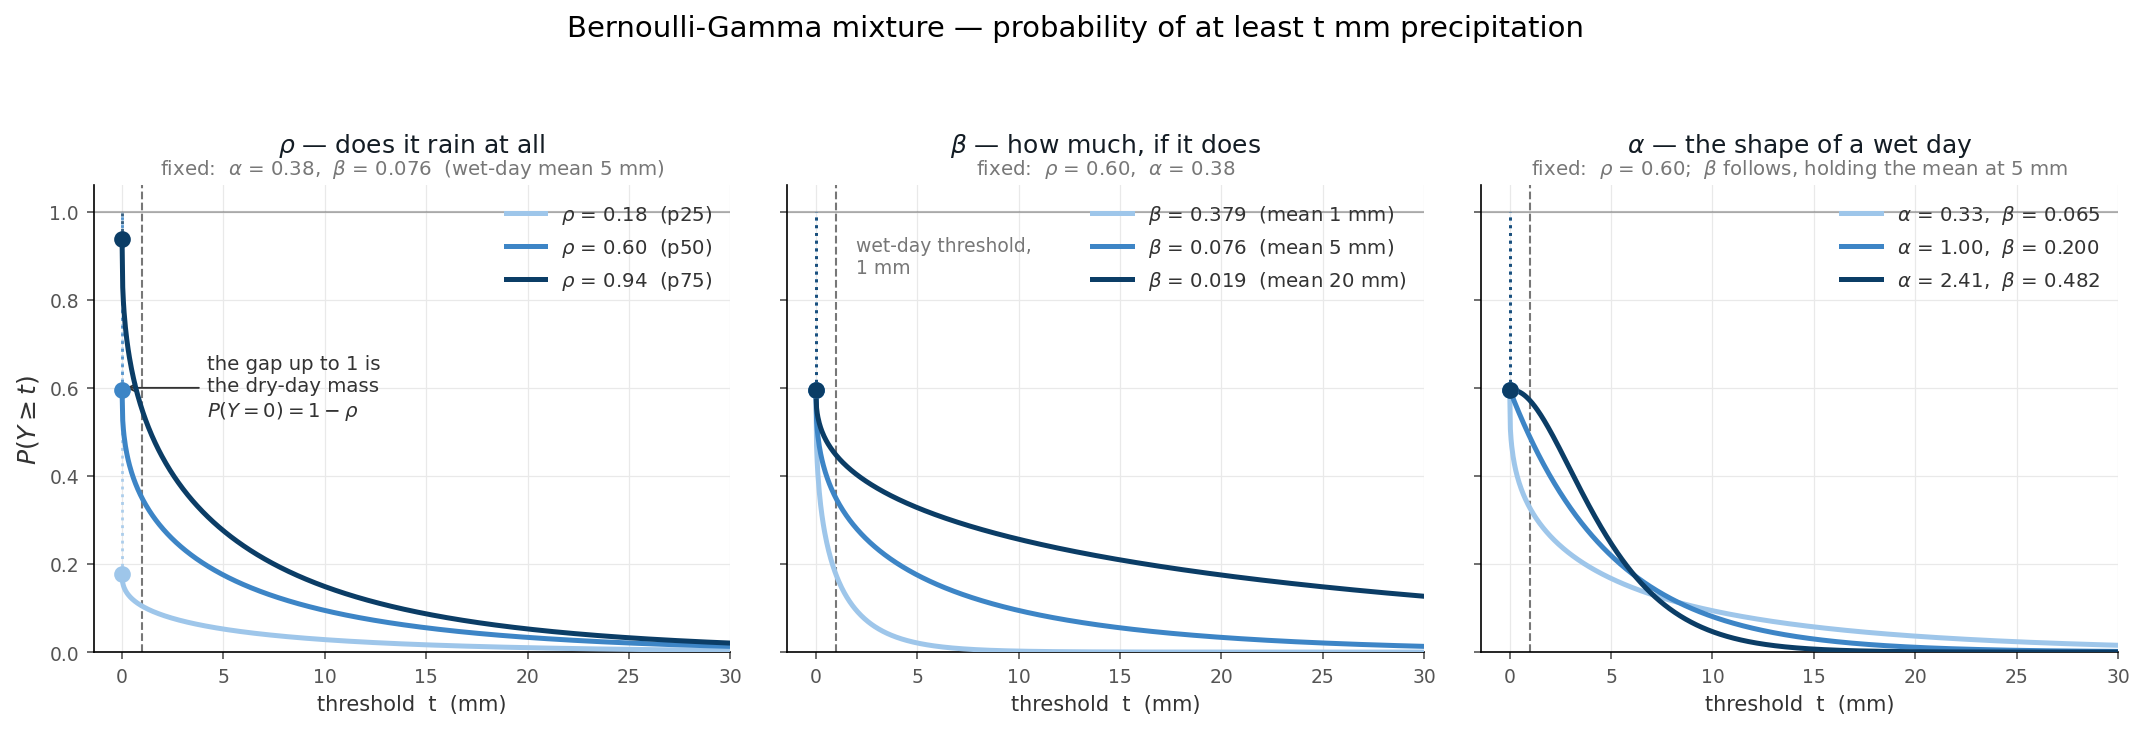
\includegraphics[width=\textwidth]{images/17_precip_wet_dry_day.png}
\caption[Bernoulli--Gamma distribution]{The Bernoulli--Gamma head read as the probability of at least $t$ millimetres, with one parameter turned per panel and the other two held constant. All parameter values are sampled from one of the model own outputs}
\label{fig:meth-precip-dials}
\end{figure}

\FloatBarrier
\section{Computational Cost}\label{sec:app-cost}

\sref{sec:meth-cost} gives the headline hardware requirement. The elevation MLP is where the cost
accumulates: it runs once per target point and never sees the input grid, and it accounts for most
of the arithmetic on both grids (\fref{fig:meth-cost-ops}). Underneath it the distance matrix holds
a fixed allocation that is far larger on the surface grid than on the atmospheric one, which is why
the atmospheric configuration is the cheaper of the two in memory as well as in operations despite
carrying many more input channels (\fref{fig:meth-cost-ops}, \fref{fig:meth-cost-mem}).

\begin{figure}[H]
    \centering
    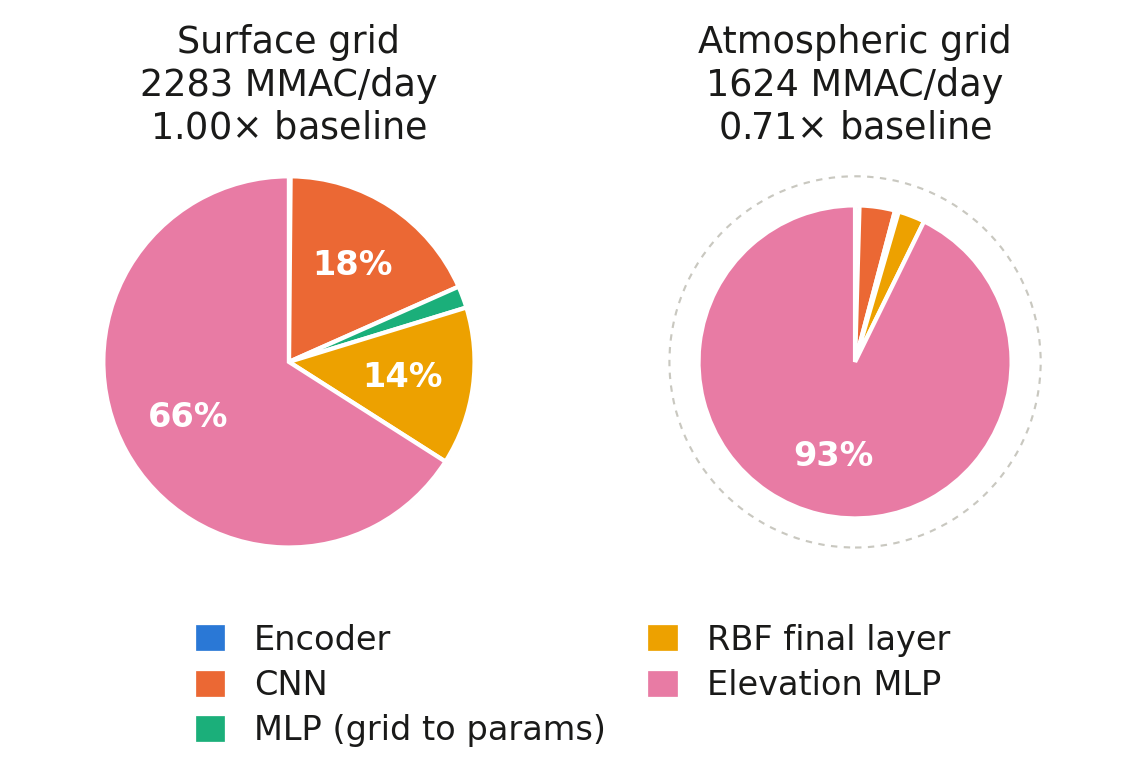
\includegraphics[width=0.75\textwidth]{images/component_cost_ops.png}
    \caption[Computational cost per component]{Computational cost per component: multiply-accumulate operations of one day, in millions, split into the architectural components.}
    \label{fig:meth-cost-ops}
\end{figure}

\begin{figure}[H]
    \centering
    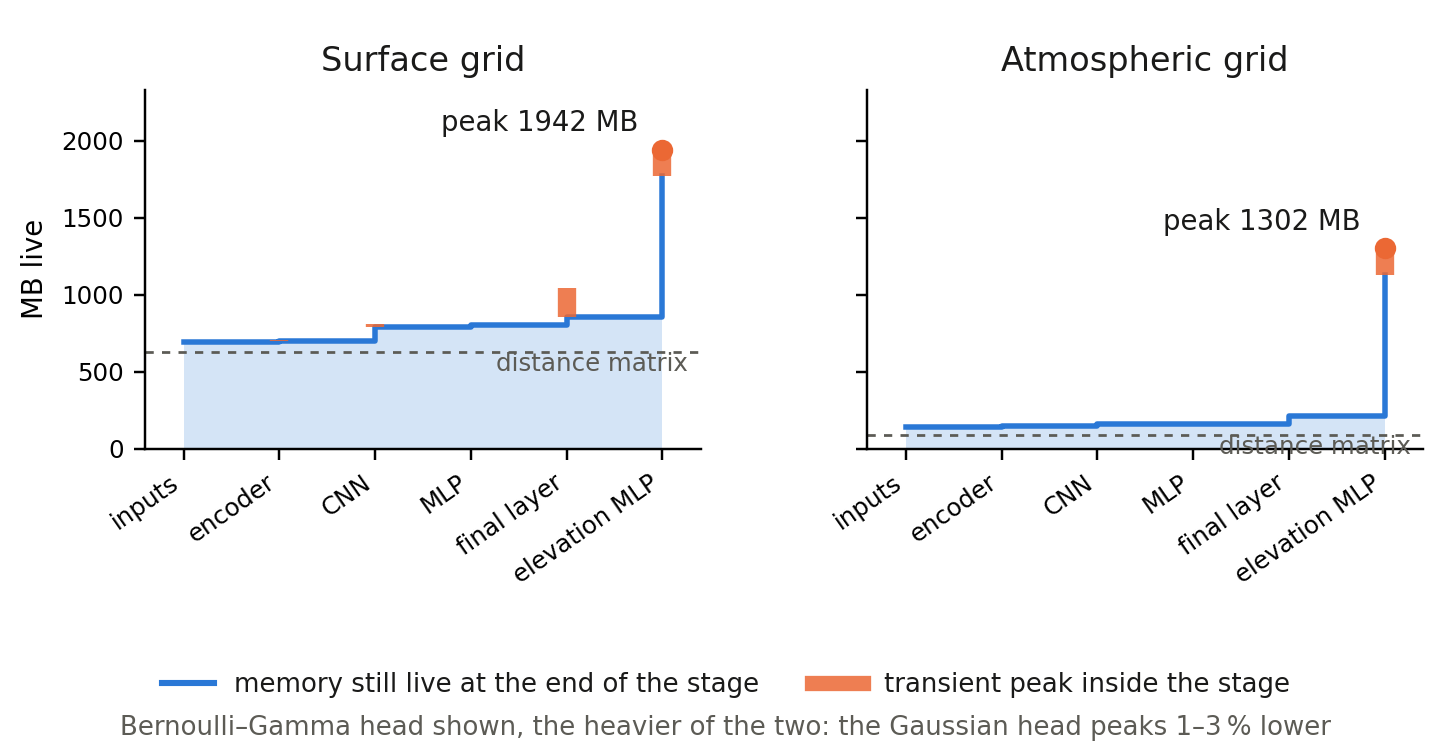
\includegraphics[width=0.86\textwidth]{images/component_cost_mem_profile.png}
    \caption[Memory through a training forward pass]{Memory estimation live at each stage of a training forward pass of the Bernoulli--Gamma configurations, the heavier of the two output heads, at the batch of eight days used in this work, with the transient inside each stage drawn above it. The peak is a moment inside a single stage, not a sum over stages.}
    \label{fig:meth-cost-mem}
\end{figure}

\FloatBarrier
\section{Additional Metric Definitions}\label{sec:app-metrics}

The metrics reported in this work are summarised in \tref{tab:meth-metrics-summary} and given in
full in \tref{tab:app-metrics-overview} below. Their definitions follow, together with the
properties of each that matter for reading \cref{ch:single-model}.

{\footnotesize
\begin{longtable}{|>{\raggedright\arraybackslash}p{3.1cm}|>{\raggedright\arraybackslash}p{0.6cm}|>{\raggedright\arraybackslash}p{3.3cm}|>{\raggedright\arraybackslash}p{6.3cm}|}
    \caption[Evaluation metrics in full]{Every metric \emph{reported} in this work, in full; \tref{tab:meth-metrics-summary} gives the short form.  Var: \textbf{T}emperature, \textbf{P}recipitation, or both. Range gives the theoretically possible values and the optimal direction.}
    \label{tab:app-metrics-overview} \\
    \hline
    \textbf{Metric} & \textbf{Var} & \textbf{Range (best)} & \textbf{Significance and use} \\
    \hline
    \endfirsthead
    \multicolumn{4}{l}{\textit{Table \thetable\ -- continued from previous page}} \\
    \hline
    \textbf{Metric} & \textbf{Var} & \textbf{Range (best)} & \textbf{Significance and use} \\
    \hline
    \endhead
    \hline
    \multicolumn{4}{r}{\textit{continued on next page}} \\
    \endfoot
    \hline
    \endlastfoot
        \multicolumn{4}{|l|}{\textit{Deterministic --- score the central prediction only}} \\
        \hline
        MAE (mean absolute error) & T, P & $[0,\infty)$, lower; in the variable's unit ($^{\circ}\mathrm{C}$ or $\mathrm{mm}$) & Headline error against the fixed truth; comparable across every run \\
        \hline
        RMSE (root-mean-square error) & T & $[0,\infty)\,^{\circ}\mathrm{C}$, lower & Same comparison, weighted towards large errors \\
        \hline
        Bias & T & $(-\infty,\infty)\,^{\circ}\mathrm{C}$, ideal $0$ & Tests for a systematic offset, using $n_{\mathrm{eff}}$ (\eref{eq:neff}) \\
        \hline
        MAE skill & P & $(-\infty,1]$, higher; $1$ perfect, $0$ = no better than ERA5-Land, negative worse & Deterministic-error skill vs.\ ERA5-Land (\eref{eq:mae-skill}); the one skill score built from a deterministic error rather than a proper score \\
        \hline
        Spearman $r_{S}$ (pooled) & P & $[-1,1]$, higher & Rank correlation between the predicted mean and the observation over the pooled point-days, subsampled to two million pairs with a fixed seed.  \\
        \hline
        \multicolumn{4}{|l|}{\textit{Probabilistic --- score the whole predictive distribution}} \\
        \hline
        CRPS (continuous ranked probability score) & T, P & $[0,\infty)$, lower; in the variable's unit ($^{\circ}\mathrm{C}$ or $\mathrm{mm}$) & The central proper score (\eref{eq:crps}) and the backbone of CRPSS below \\
        \hline
        CRPSS (CRPS skill score) & T & $(-\infty,1]$, higher; $1$ perfect, $0$ = baseline & CRPS-based skill vs.\ the bilinear input (\eref{eq:crpss}); comparable whenever the reference is shared\\
        \hline
        BSS (Brier skill score) & P & $(-\infty,1]$, higher; $1$ perfect, $0$ = baseline & Event skill: how much better the predicted probability of the binary event ``accumulation $\geq t$'' is than ERA5-Land's, at one threshold $t$ at a time (\eref{eq:bss}) \\
        \hline
        RPSS (ranked probability skill score) & P & $(-\infty,1]$, higher; $1$ perfect, $0$ = baseline & Whole-distribution categorical skill (\eref{eq:rpss}); penalises misplaced probability mass \\
        \hline
        R01 (wet-day frequency) & P & ratio, ideal $1$ & Predicted over observed fraction of days $\geq 1\,\mathrm{mm}$; the model's fraction is the analytic $P(Y \geq 1\,\mathrm{mm})$ of \eref{eq:bg-exceedance} evaluated at every target point and day, then averaged over them \\
        \hline
        Dry-day fraction & P & $[0,1]$, ideal $=$ observed & Fraction of days below $0.1\,\mathrm{mm}$; the model's value is $1 - P(Y \geq 0.1\,\mathrm{mm})$ evaluated at every target point and day, then averaged over them \\
        \hline
        SDII (simple daily intensity index) & P & $[0,\infty)\,\mathrm{mm}$, ideal $=$ observed & Mean accumulation on wet days. The model's value is the \emph{pooled} analytic wet-day intensity, $\sum \mathbb{E}[Y\,\mathbf{1}\{Y \geq 1\,\mathrm{mm}\}] \big/ \sum P(Y \geq 1\,\mathrm{mm})$ over all point-days \\
        \hline
        R10 & P & $[0,1]$, ideal $=$ observed & Fraction of days with accumulation $>10\,\mathrm{mm}$, strictly greater for the observations and the model alike. The model's value is the fraction of draws sampled from the predictive distribution that exceed $10\,\mathrm{mm}$, pooled over every target point and day \\
        \hline
        P98 & P & $[0,\infty)\,\mathrm{mm}$, ideal $=$ observed & 98th percentile of wet-day accumulation. The model's value is one percentile of the \emph{pooled} cloud of wet draws over all target points and days, not an average of per-point-day percentiles \\
        \hline
        PIT (probability integral transform) & T, P& Mean $[0,1]$, ideal $0.5$;\newline SD $[0,0.5]$, ideal $1/\sqrt{12}\approx0.289$ & Calibration diagnostic: whether the predicted quantiles are correct, read from a PIT histogram or Q--Q plot against the uniform. \\
        \hline
        Standardised-error SD & T & $[0,\infty)$, ideal $1$;\newline $<1$ forecast over-dispersed (predicted spread too wide),\newline $>1$ over-confident & Calibration diagnostic: whether the predicted spread matches the actual error spread \\
        \hline
        Coverage ($50\,\%$, $90\,\%$) & T & $[0,1]$,\newline ideal $=$ nominal\newline ($0.50$/$0.90$) & Calibration diagnostic: fraction of observations inside the nominal central interval \\
        \hline
\end{longtable}
}

\begin{table}[htbp]
    \centering
    \caption[Aggregation levels]{Aggregation levels. Within a regime (\sref{subsec:meth-cv}), the same
    metric can be read at any of these levels; the level is stated wherever a number is quoted.}
    \label{tab:app-eval-regimes}
    \footnotesize
    \begin{tabular}{|p{3.0cm}|p{10.3cm}|}
        \hline
        Pooled & Every valid target point and day of the regime is flattened into one array and averaged in a single pass, giving the headline number. A ratio-valued score is pooled as a ratio of the two pooled averages, never as an average of ratios \\
        \hline
        Per target point & Pooled over days only, giving a map. Whether its domain mean returns the pooled number depends on the metric: it does for MAE and bias, which are linear in the point-days, as long as every point carries the same number of valid days; it does not for RMSE, because a mean of square roots is not the square root of a mean; and it does not for any ratio-valued score (CRPSS, BSS, RPSS, MAE skill, R01, SDII), whose pooled and per-point forms are different quantities. The map is therefore read for \emph{where}, and the pooled number quoted for \emph{how much} \\
        \hline
        Per day & Pooled over target points only, into one domain-mean value per day; the basis of the bias significance test and of the monthly curves in \cref{ch:single-model} \\
        \hline
        Per fold (CV holdout only) & The pooled metric broken out by the five separately trained folds; the resulting spread distinguishes a stable ranking from one that should not be read too literally (\sref{subsec:single-precip-headline} uses it this way) \\
        \hline
    \end{tabular}
\end{table}

\subsection{Deterministic Errors and the CRPS}\label{subsec:app-crps}

\paragraph*{Standard error of the bias.}
Whether a mean error differs from zero cannot be judged by pooling every point and every day: the field is smooth and successive days are linked by the weather, so a nominal sample size of tens of millions would make any offset significant. Each day is therefore collapsed to its domain mean first, and the remaining serial correlation is absorbed into the effective sample size
\begin{equation}
    n_{\mathrm{eff}} \;=\; T \, \frac{1 - r_{1}}{1 + r_{1}} ,
    \label{eq:neff}
\end{equation}
with $T$ the number of days and $r_1$ the lag-1 autocorrelation of the daily series~\cite{wilks2019statistical}. Confidence intervals and $t$ tests use $n_{\mathrm{eff}}$ in place of $T$, which widens the standard error of the mean by a factor set entirely by $r_1$,
\begin{equation}
    \mathrm{SE}_{\mathrm{adj}} \;=\; \frac{s}{\sqrt{n_{\mathrm{eff}}}}
    \;=\; \frac{s}{\sqrt{T}} \sqrt{\frac{1 + r_1}{1 - r_1}}
    \;=\; \mathrm{SE} \, \sqrt{\frac{1 + r_1}{1 - r_1}} ,
    \label{eq:se-adj}
\end{equation}
where $s$ is the standard deviation of the daily means. Persistence is therefore paid for directly in interval width, and an offset has to clear a correspondingly higher bar before it counts as real: at $r_1 = 0.6$ the interval doubles, and at the autocorrelation of the 2024 holdout, which leaves about $220$ of its $366$ days effectively independent (\sref{subsec:single-tmax-discussion}), it widens by roughly $30\,\%$. This stops trivial noise from being labelled statistically significant merely because the pooled sample is large. The correction covers day-to-day persistence but not seasonal structure, so its intervals stay mildly optimistic. The daily series, $r_1$, $n_{\mathrm{eff}}$ and the resulting interval are produced by \texttt{scripts/gen\_bias\_significance.py} from the cached predictions of the regime being scored, one JSON per model and regime.

\paragraph*{Continuous ranked probability score (CRPS).}
The central probabilistic score is the continuous ranked probability score (CRPS)~\cite{gneiting2007scoring}, for a predictive CDF $F$ and an observation $y$
\begin{equation}
    \mathrm{CRPS}(F, y) \;=\; \int_{-\infty}^{\infty} \bigl( F(z) - \mathbf{1}\{z \geq y\} \bigr)^{2} \,\mathrm{d}z ,
    \label{eq:crps}
\end{equation}
the squared distance between the predicted CDF and the step function of the observation, strictly proper so that it rewards distributions that are both sharp and calibrated. It is closed-form for the Gaussian; for the Bernoulli--Gamma it is sample-estimated during training, while the station evaluation uses the closed form of the Gamma CRPS. For a deterministic forecast $x$ it collapses to $\lvert x - y \rvert$, so a probabilistic model and a deterministic baseline can be scored on one scale, which is the property every skill score below relies on.

\paragraph*{Probability integral transform (PIT).}
Calibration is assessed through the probability integral transform: if the predictive distributions are correct, the values $u = F(y)$ are uniform on $[0,1]$. The mixed distribution of precipitation needs one adjustment at its point mass (\sref{subsec:app-skill-precip}).

\subsection{Temperature Skill and Calibration}\label{subsec:app-skill-tmax}

\paragraph*{Skill against the interpolated input (CRPSS).}
The temperature reference forecast is the ERA5-Land daily maximum $2\,\mathrm{m}$ temperature field, $\mathrm{t2m\_max}$ on the $0.1^{\circ}$ grid of \tref{tab:data-grids}, bilinearly interpolated to the MeteoSwiss target points. This product is not the input grid of every model: the atmospheric configurations read ERA5 at $0.25^{\circ}$ and never see a surface field at all, so their reference is loaded separately rather than taken from their own context. Being deterministic, its CRPS equals its absolute error, and
\begin{equation}
    \mathrm{CRPSS} \;=\; 1 - \frac{\overline{\mathrm{CRPS}}_{\mathrm{model}}}{\overline{\mathrm{CRPS}}_{\mathrm{ref}}}
    \label{eq:crpss}
\end{equation}
is computed pooled and per target point, the map showing \emph{where} the model beats interpolation. Two runs are CRPSS-comparable only if they share the same reference construction: the same baseline file, the same target points and the same domain bounds. That condition is weaker than sharing an input grid, and satisfying it makes the comparison in \cref{ch:single-model} legitimate. Every temperature configuration in this work, surface and atmospheric alike, is scored against one and the same interpolated ERA5-Land field, so its CRPSS values differ from each other only through the numerator.

\paragraph*{Calibration of the Gaussian head.}
The PIT of \sref{subsec:app-crps} applies unchanged to the Gaussian. Two further diagnostics of \tref{tab:app-metrics-overview} are defined here rather than there because they are available for temperature only: both need a predicted mean and a predicted spread, and the Bernoulli--Gamma head of \sref{subsec:meth-likelihoods} carries neither as a parameter, so precipitation calibration rests on the PIT alone. The first standardises every error by the spread predicted at that point and day, $z = (y - \mu)/\sigma$. If the predicted spread is right, $z$ has a standard deviation of one; a value below one means the model predicts wider intervals than its errors require, a value above one that it is over-confident. The second is the central coverage: the fraction of observations falling inside the nominal $50\,\%$ and $90\,\%$ interval of the predictive distribution, read off the PIT values as the fraction landing in $[0.25, 0.75]$ and $[0.05, 0.95]$. Both are pooled over every valid target point and day of the regime, and both are reported alongside the PIT moments in the calibration figures of \cref{ch:single-model}.

\subsection{Precipitation Indices and Event-Based Skills}\label{subsec:app-skill-precip}

\paragraph*{Physical indices instead of squared error.}
Squared-error measures summarise daily precipitation poorly: the field is zero on most days and heavily skewed on wet days, while what matters is occurrence, intensity and extremes. Following \textcite{vaughan2022convcnp}, the precipitation models are judged on the physical indices of \tref{tab:app-metrics-overview}. No wet/dry classification with a fixed probability cut is ever applied. Wherever an occurrence statistic can be, it is instead read from the exceedance probability of \eref{eq:bg-exceedance}, evaluated at the threshold that statistic is defined by: $1\,\mathrm{mm}$ for the wet-day frequency and R01, $0.1\,\mathrm{mm}$ for the dry-day fraction, and each of the four thresholds of the Brier skill maps below. Note that these are two different cuts and are kept apart throughout: $1\,\mathrm{mm}$ is the wet-day definition this chapter and its indices are built on, while $0.1\,\mathrm{mm}$ is the any-rain cut separating a dry day from drizzle. The next paragraph gives the route taken by the indices that have no such closed form.

\paragraph*{From point-day distributions to pooled frequencies.}
\fref{fig:meth-precip-dials} reads the distribution at a single point and day, whereas the results report \emph{frequencies} pooled over many points and days. Two routes turn one into the other. Where the quantity has a closed form in $(\rho, \alpha, \beta)$, the per-point-day probability \emph{is} that day's contribution to the event's rate, so averaging it gives the frequency exactly; this is how R01 and the wet-day-frequency maps are read off. Where no closed form exists, as for R10, P98 and the intensity categories, the model is sampled at each point and day and the frequency or percentile computed from those draws as it would be from observations.

\paragraph*{PIT at the point mass.}
The probability integral transform of \sref{subsec:app-crps} needs one adjustment for a distribution that puts finite probability on the single value zero. It takes the standard randomisation at that point mass, drawing $u$ uniformly from $[0, 1-\rho]$ whenever the observed day is dry ($y \leq 0.05\,\mathrm{mm}$), so that a correct model still returns uniform values.

\paragraph*{Brier skill score (BSS).}
The precipitation skill scores are event-based~\cite{wilks2019statistical} against the ERA5-Land total precipitation field, bilinearly interpolated and treated as a deterministic forecast. All three of them, the Brier skill here, the MAE skill and the RPSS below, are scored against a reference re-accumulated over the same $06$--$06\,\mathrm{UTC}$ window as RhiresD rather than over the UTC calendar day, so reference and target cover the same twenty-four hours. This is deliberately not the field the model reads: the input channel keeps the calendar-day total of \sref{subsec:data-coords}, and only the scoring reference is rebuilt on the target's window. The model issues $P(Y \geq t)$, scored by the Brier score $\mathrm{BS} = \overline{(p - o)^{2}}$ with $o \in \{0,1\}$ the observed event, giving
\begin{equation}
    \mathrm{BSS} \;=\; 1 - \frac{\mathrm{BS}_{\mathrm{model}}}{\mathrm{BS}_{\mathrm{ref}}}
    \label{eq:bss}
\end{equation}
mapped per target point at $t \in \{0.1, 10, 40, 80\}\,\mathrm{mm}$, from any-rain to the heavy tail. One property of the score has to be carried into any summary of the map. Where the reference never errs on the event, $\mathrm{BS}_{\mathrm{ref}} = 0$ and the ratio is undefined, so those target points are dropped rather than counted as a tie. They are the points the reference finds easiest, which means a domain median or mean of the BSS map is taken over a subset from which the reference's best-served locations have been removed.

\paragraph*{MAE skill.}
Since MAE is reported for every run, it can be scored against the same reference,
\begin{equation}
    \mathrm{MAE\text{-}skill} \;=\; 1 - \frac{\mathrm{MAE}_{\mathrm{model}}}{\mathrm{MAE}_{\mathrm{ref}}} ,
    \label{eq:mae-skill}
\end{equation}
which unlike BSS and RPSS scores only the central prediction, a difference that matters since \sref{subsec:single-precip-headline} finds it disagrees in sign with RPSS.

That disagreement is not an accident of the data, and the definition of the central prediction is where it starts. The point forecast entering both the MAE and the rank correlation is the mixture mean $\mathbb{E}[Y] = \rho\,\alpha/\beta$, the like-for-like counterpart of the single value the deterministic reference issues. But the absolute error is minimised by the \emph{median}, not the mean, and for a distribution with most of its mass at zero the two are far apart: a model that honestly reports a $40\,\%$ chance of $8\,\mathrm{mm}$ returns a mean of about $3\,\mathrm{mm}$ on a day that will most likely stay dry. Reporting the median instead would lower every run's MAE, but it would also throw away the amount the model is least sure about, and it would no longer be the quantity the reference is compared against. The mean is kept, and the resulting penalty is understood as the price a distribution pays when it is scored by a metric that rewards the safest single number.

\paragraph*{Ranked probability skill score (RPSS).}
To judge the intensity structure as a whole, the accumulation is divided into the ordered categories $[0, 0.1)$, $[0.1, 10)$, $[10, 40)$, $[40, 80)$ and $[80, \infty)\,\mathrm{mm}$ and scored with the ranked probability score, the squared distance between the forecast and observed CDFs accumulated over the internal boundaries $t_k$:
\begin{equation}
    \mathrm{RPS} \;=\; \sum_{k} \bigl( F(t_k) - \mathbf{1}\{y < t_k\} \bigr)^{2},
    \qquad
    \mathrm{RPSS} \;=\; 1 - \frac{\overline{\mathrm{RPS}}_{\mathrm{model}}}{\overline{\mathrm{RPS}}_{\mathrm{ref}}} .
    \label{eq:rpss}
\end{equation}
Both are reported per target point and pooled over the domain.
\FloatBarrier
\section{Temperature Model Metrics}\label{sec:app-tmax-metrics}

The headline metrics of the seven temperature runs are given in \tref{tab:single-tmax-headline} of \cref{ch:single-model}; the figures below support them.


\begin{figure}[H]
\centering
\subfloat[against target altitude]{%
  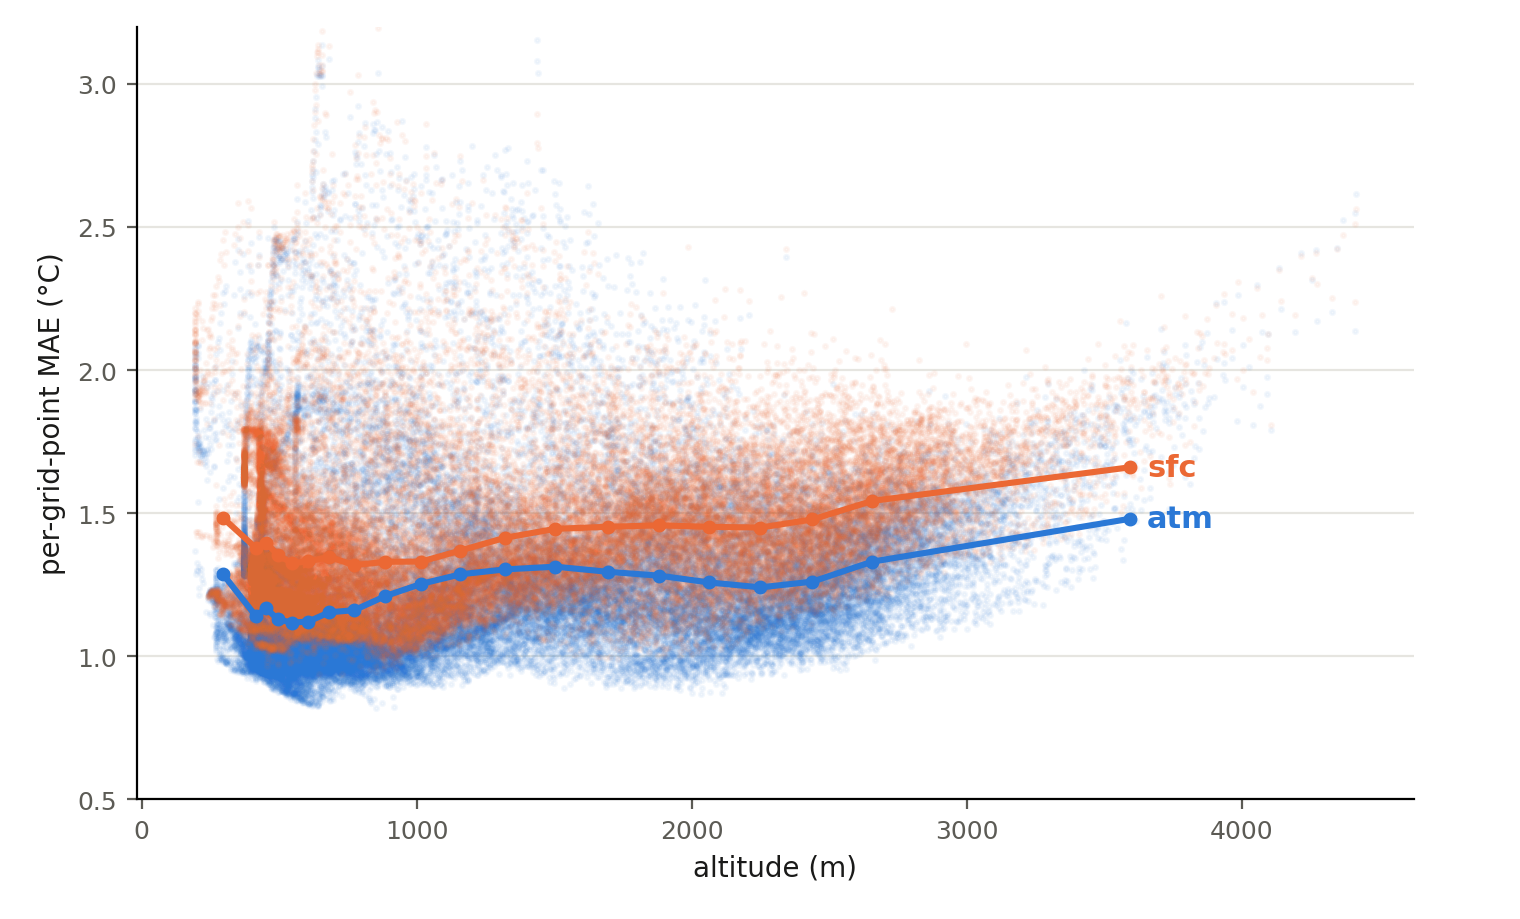
\includegraphics[width=0.49\textwidth]{images/tmax_mae_vs_altitude_overlay_cv.png}}
\hfill
\subfloat[against elevation mismatch, logarithmic axis]{%
  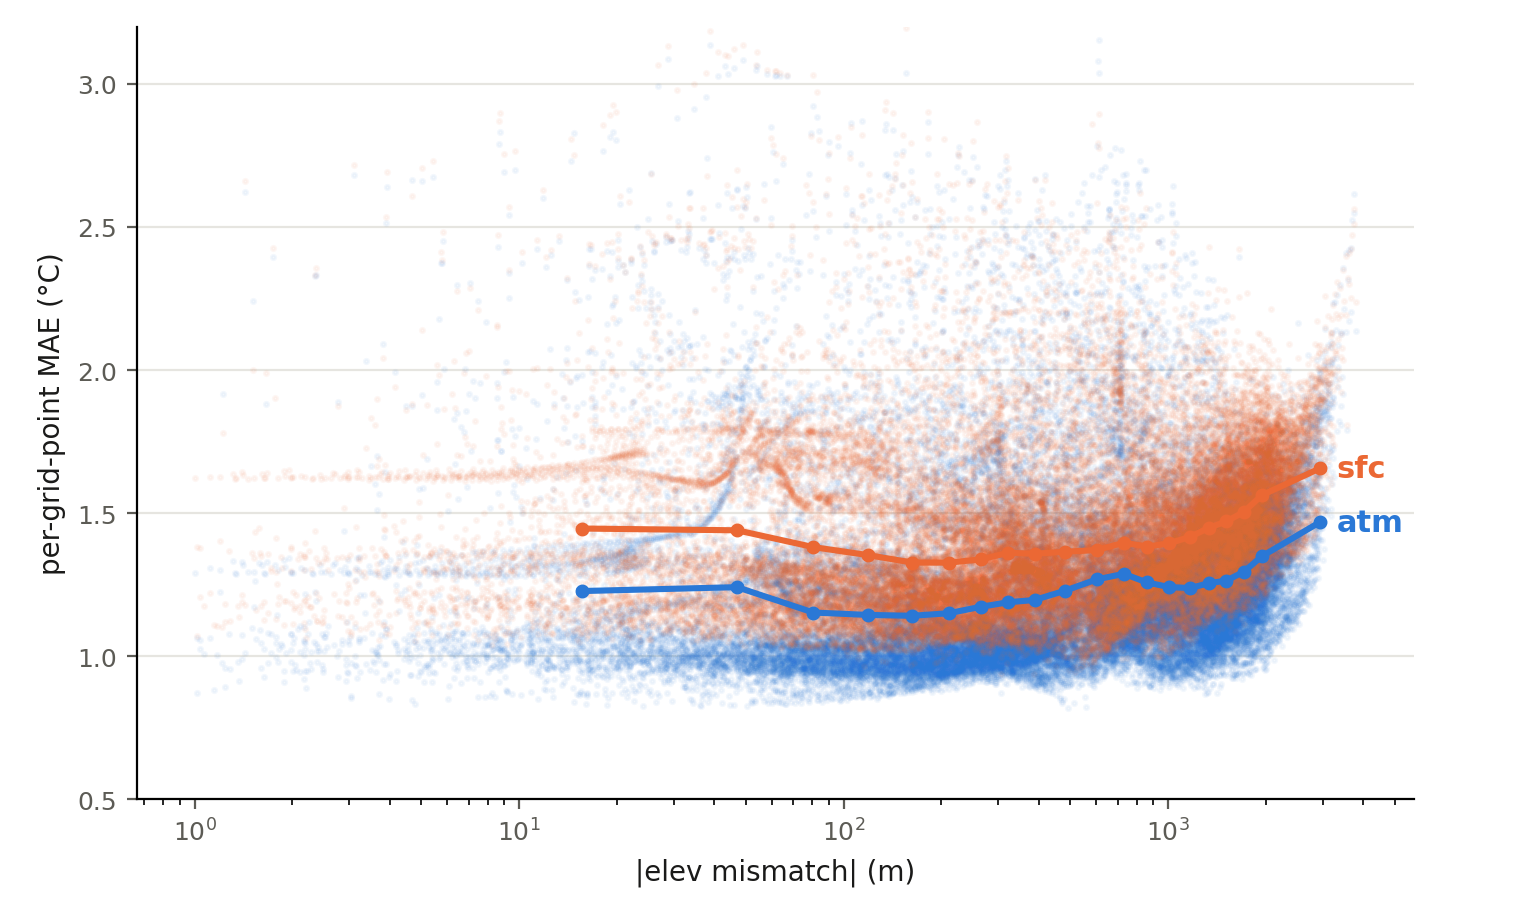
\includegraphics[width=0.49\textwidth]{images/tmax_mae_vs_elevmismatch_overlay_cv.png}}
\caption[Per-pixel error against altitude and against elevation mismatch]{Per-grid-point MAE over the CV holdout against altitude and against elevation mismatch, for \texttt{sfc} and \texttt{atm} (\sref{subsec:single-tmax-geography}). Every grid point is plotted; the heavy line is the binned median. The panels differ only in the horizontal variable.}
\label{fig:single-tmax-terrain}
\end{figure}

\begin{figure}[H]
\centering
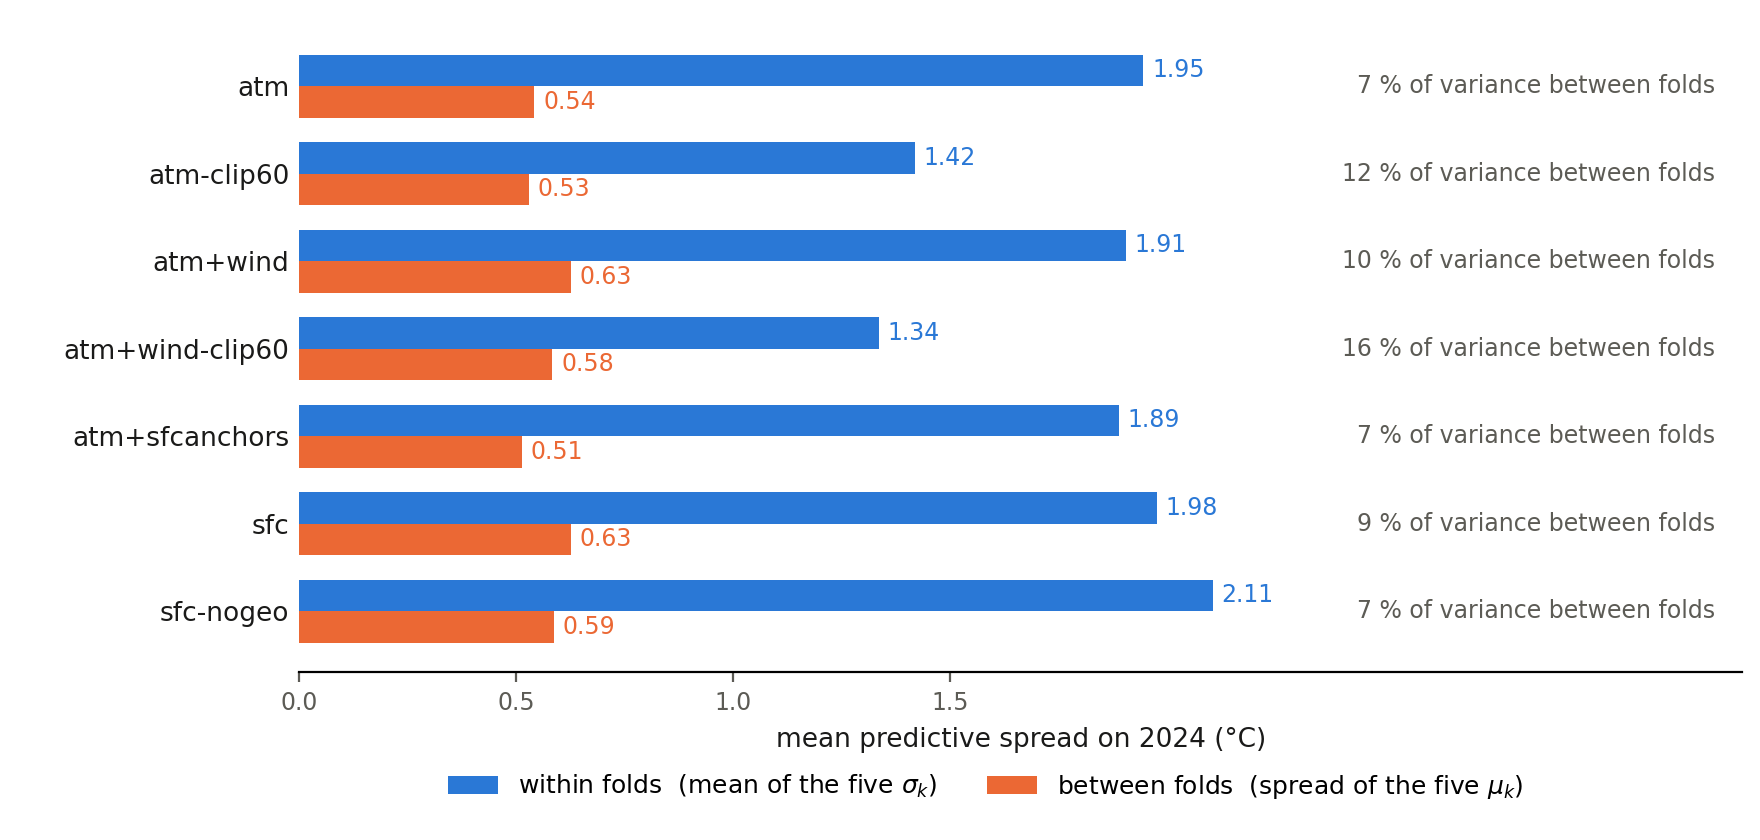
\includegraphics[width=0.9\textwidth]{images/tmax_sigma_decomposition.png}
\caption[Decomposition of the 2024 predictive spread, all models]{Decomposition of the mean 2024 predictive spread into its two moment-matching parts for all seven temperature models: the mean single-fold spread and the disagreement of the five fold means. The selected model \texttt{atm+wind-clip60} carries the largest between-fold variance of $16\,\%$ }
\label{fig:app-sigma-decomposition}
\end{figure}

\begin{figure}[H]
\centering
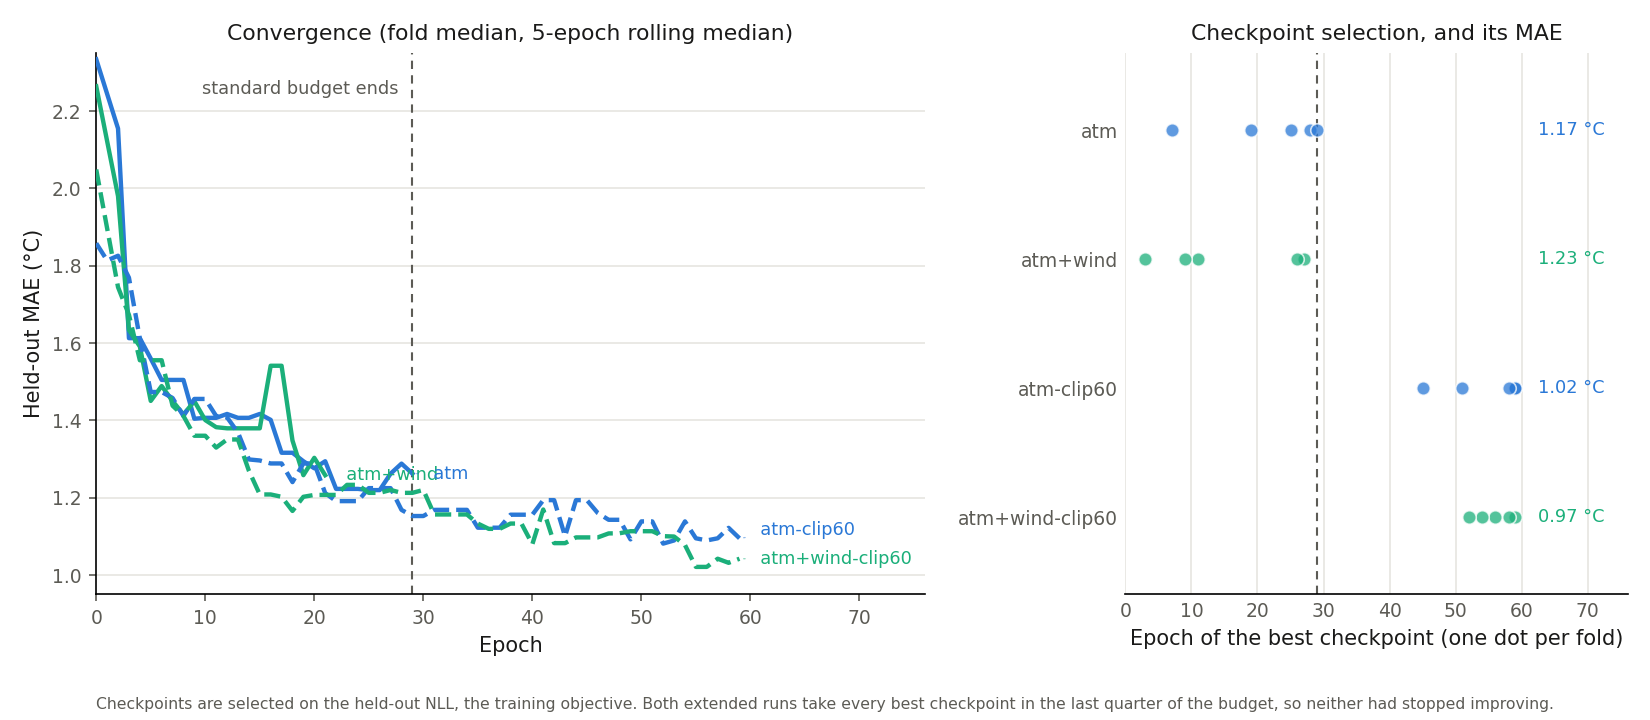
\includegraphics[width=\textwidth]{images/tmax_convergence_wind.png}
\caption[Convergence of the wind ablation under both training budgets]{Convergence of the two
atmospheric configurations with and without the wind channels, under the standard and the extended
training budget. Left: the held-out score written at each epoch during training, as the median over
the five folds and smoothed with a five-epoch rolling median, since the epoch-to-epoch scatter is
larger than the difference between the runs. Right: the epoch at which each fold's best checkpoint
was taken, one dot per fold, with the median held-out MAE of those checkpoints beside it. Selection
is on the held-out negative log-likelihood, the training objective, so the right panel is the
quantity that actually decided which weights entered \cref{ch:single-model}. At the standard budget
the wind model is behind ($1.23$ against $1.17\,^{\circ}\mathrm{C}$) and three of its five folds stop
early; under the extended budget the order reverses ($0.97$ against $1.02$) and every one of its
best checkpoints falls between epochs $52$ and $59$, so it had not stopped improving when the run
ended. The curve is a median over days while the headline MAE of \tref{tab:single-tmax-headline} is
a mean over all point-days, so the levels here are not directly comparable with that table; the
ordering and the trend are.}
\label{fig:app-tmax-convergence}
\end{figure}

Under the standard budget three of the five \texttt{atm+wind} folds stop early, whereas under the
extended one every fold of \texttt{atm+wind-clip60} takes its best checkpoint between epochs $52$ and
$59$: the run was still improving when it ended, which is why the extra channels only pay off once the
budget is long enough to incorporate them (\sref{subsec:single-tmax-headline}).

\FloatBarrier
\section{Feature Importance}\label{sec:app-fi}

Every attribution reproduced here is scored on the 2024 holdout year, the regime of
\tref{tab:meth-fi-setup}, so the permutation and LIME results can be read against each other
directly. The section is arranged in two steps: the selected models in full, including their
per-channel resolution, then every configuration side by side in one figure per method.

\subsection{Selected Models}\label{subsec:app-fi-selected}

For each selected model the two methods are placed in one figure, permutation above and LIME below,
each grouped view followed by its per-channel counterpart.

\begin{figure}[p]
\centering
\subfloat[Grouped permutation importance]{%
  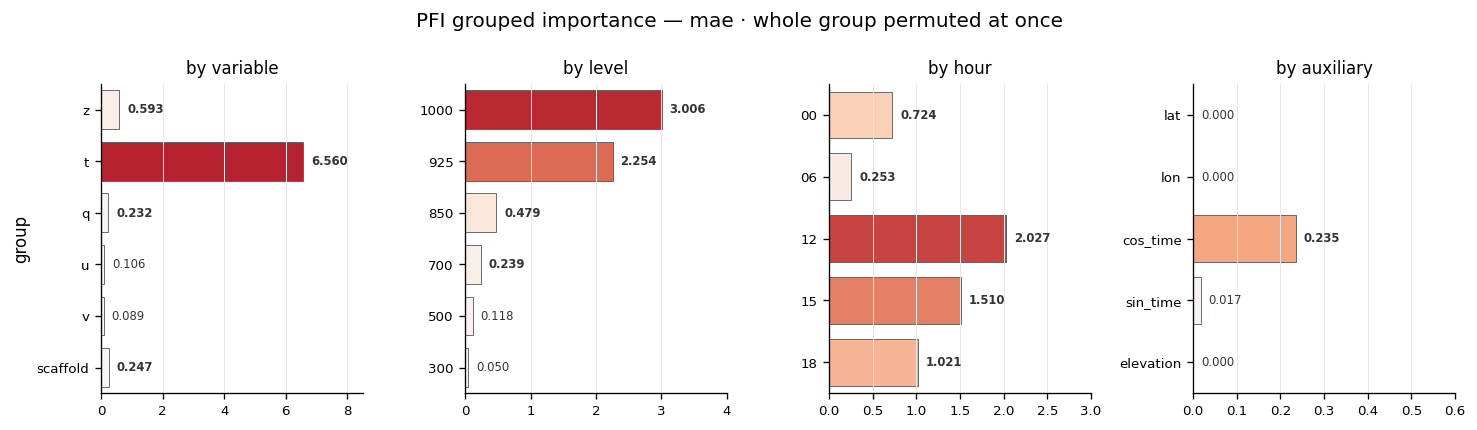
\includegraphics[width=0.84\textwidth,height=3.9cm,keepaspectratio]{images/results/tmax__pfi_groups_mae__feature_importance_2024__lbclip_wind.png}}\\[1ex]
\subfloat[Per-channel permutation importance]{%
  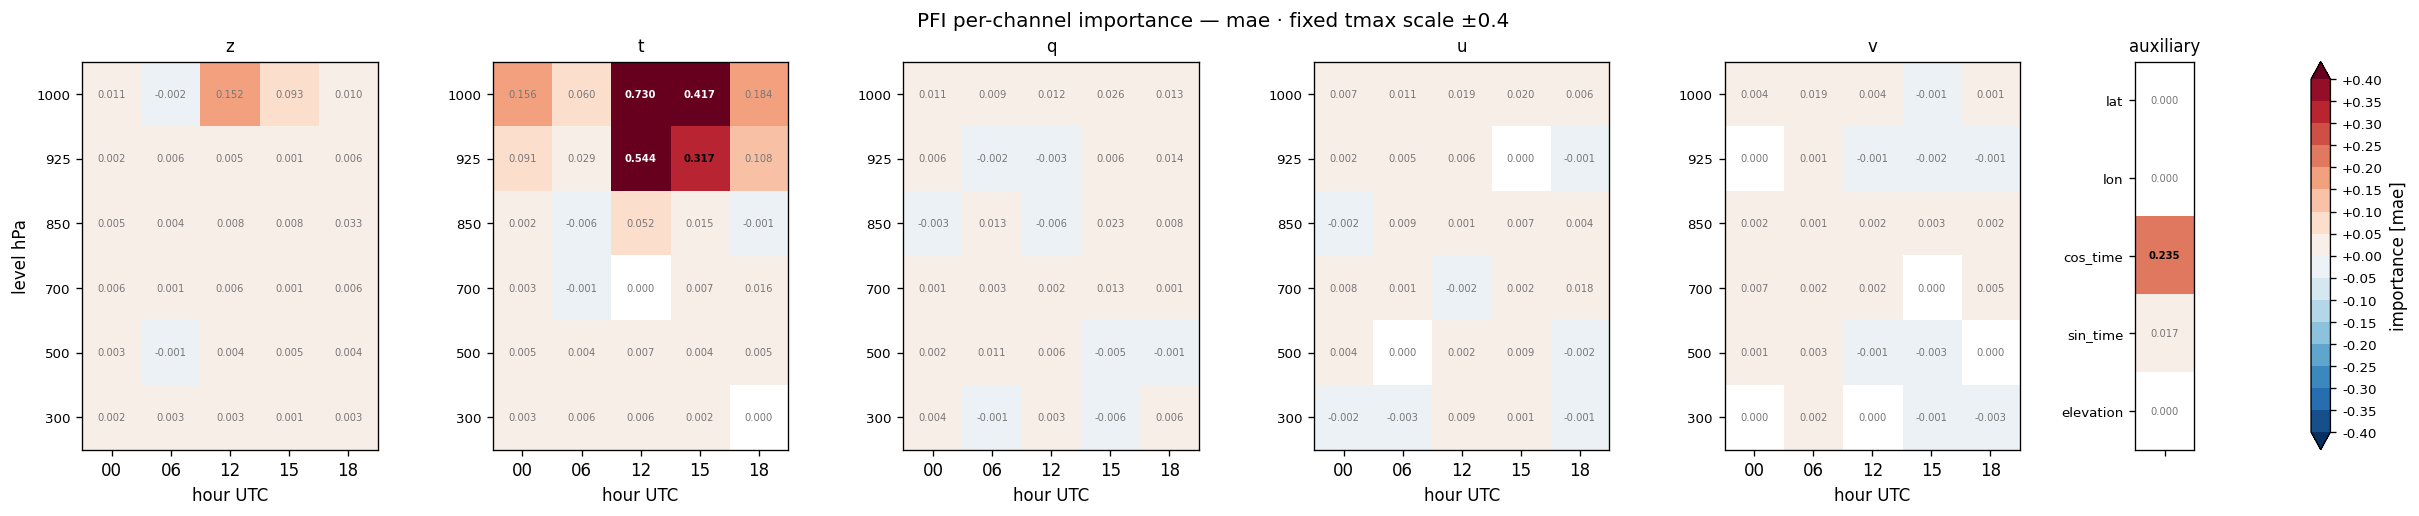
\includegraphics[width=0.84\textwidth,height=3.9cm,keepaspectratio]{images/results/tmax__pfi_heatmap_mae__feature_importance_2024__lbclip_wind.png}}\\[1ex]
\subfloat[Grouped LIME feature importance]{%
  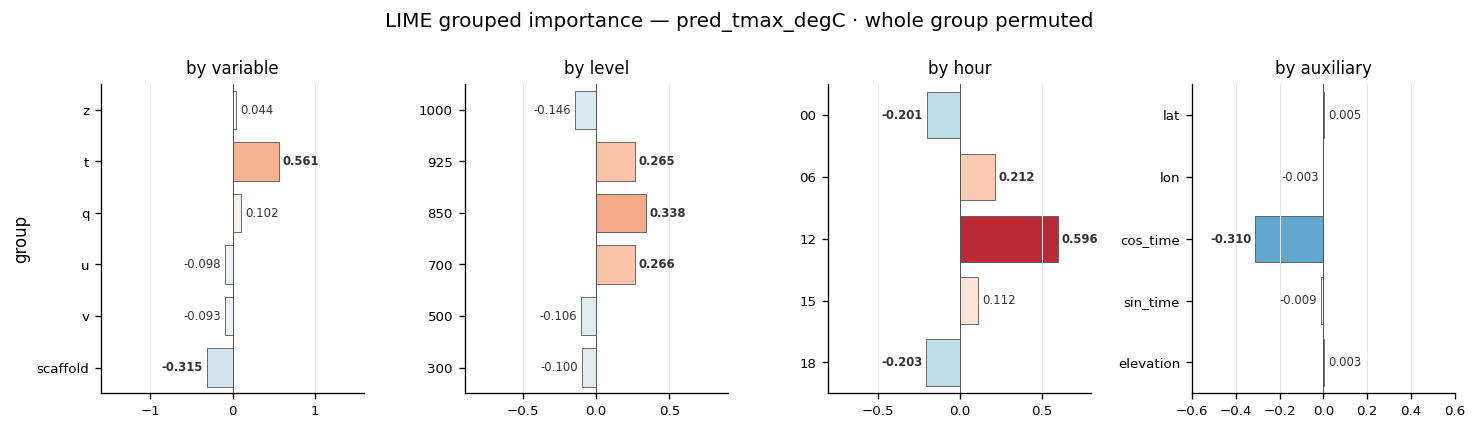
\includegraphics[width=0.84\textwidth,height=3.9cm,keepaspectratio]{images/results/tmax__lime_groups_pred_tmax_degC__feature_importance_2024__lbclip_wind.png}}\\[1ex]
\subfloat[Per-channel LIME feature importance]{%
  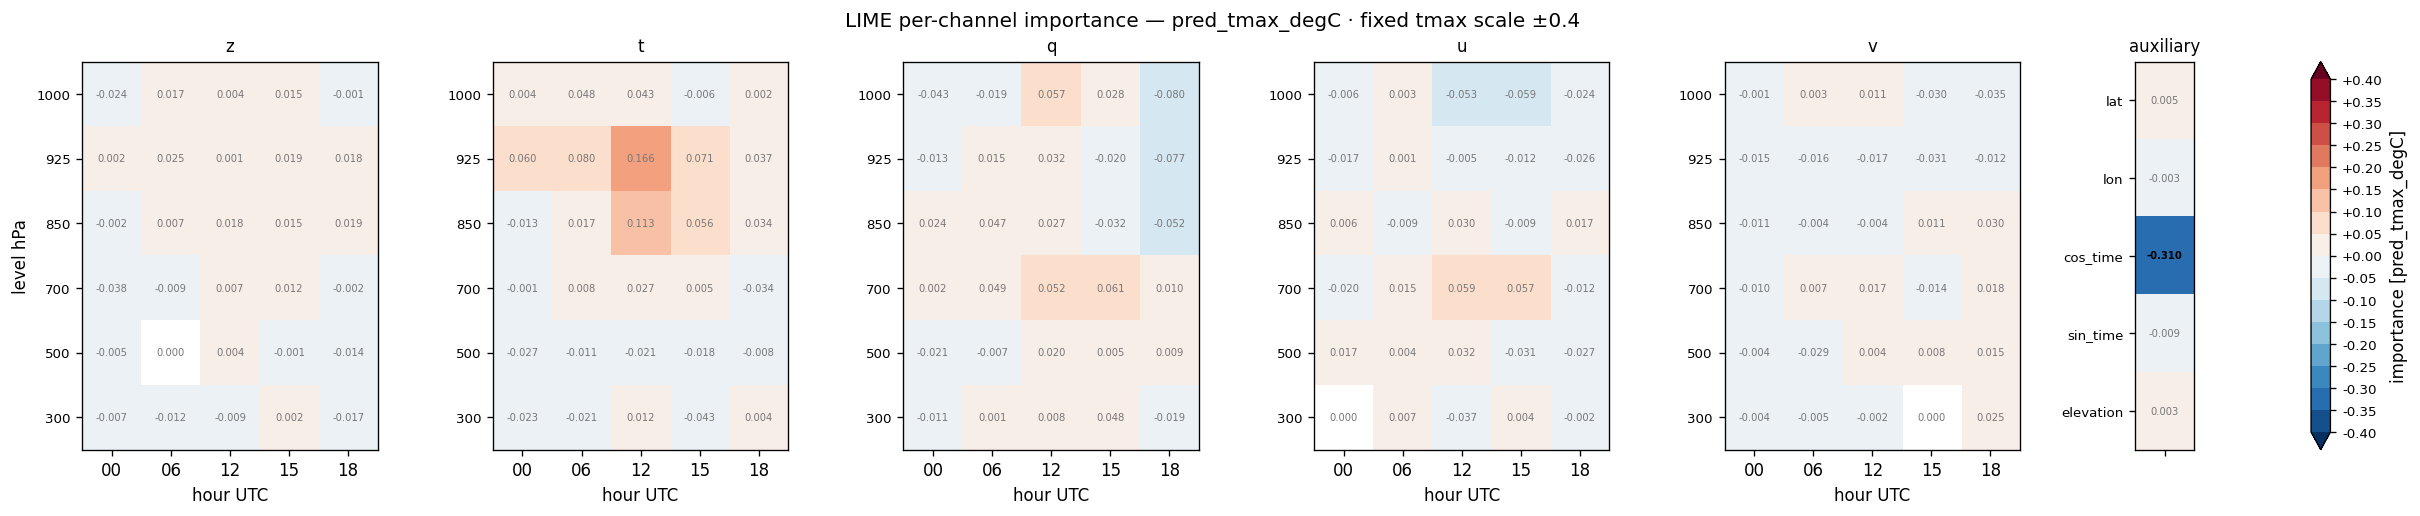
\includegraphics[width=0.84\textwidth,height=3.9cm,keepaspectratio]{images/results/tmax__lime_heatmap_pred_tmax_degC__feature_importance_2024__lbclip_wind.png}}
\caption[Feature Importance of the selected temperature model]{Feature Importance of the selected temperature model \texttt{atm+wind-clip60}. Permutation importance
is an MAE degradation in degrees Celsius, LIME a signed effect on the spatial-mean prediction in the
same unit, so the two panels of each pair share a unit but not a meaning. Temperature dominates the
grouped permutation view while the wind groups rank last among the meteorological variables, and the
level and hour patterns match the wind-free models, led by $1000$ and $925\,\mathrm{hPa}$ and the
midday hours. LIME agrees on those essentials: temperature leads, 12~UTC is the leading hour, and
the wind groups carry small coefficients. The per-channel panels are close to blank in the wind
groups at the shared scale, so no single wind channel carries visible importance on its own.}
\label{fig:app-fi-sel-tmax}
\end{figure}

\begin{figure}[p]
\centering
\subfloat[Grouped permutation importance]{%
  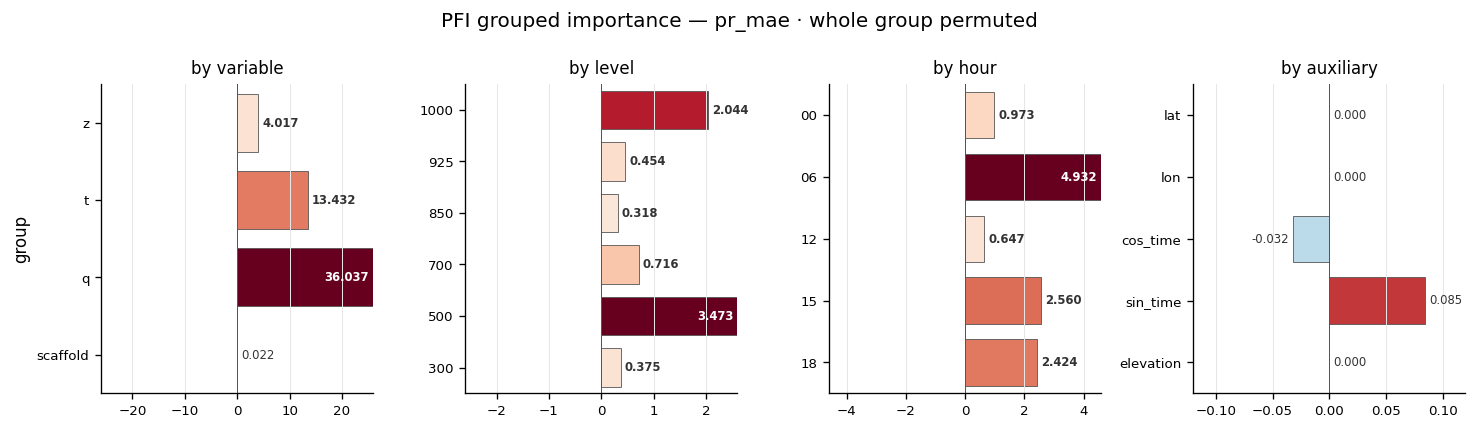
\includegraphics[width=0.84\textwidth,height=3.9cm,keepaspectratio]{images/results/precip__pfi_groups_pr_mae__feature_importance_2024__clean_solo_precip_ftcrps.png}}\\[1ex]
\subfloat[Per-channel permutation importance]{%
  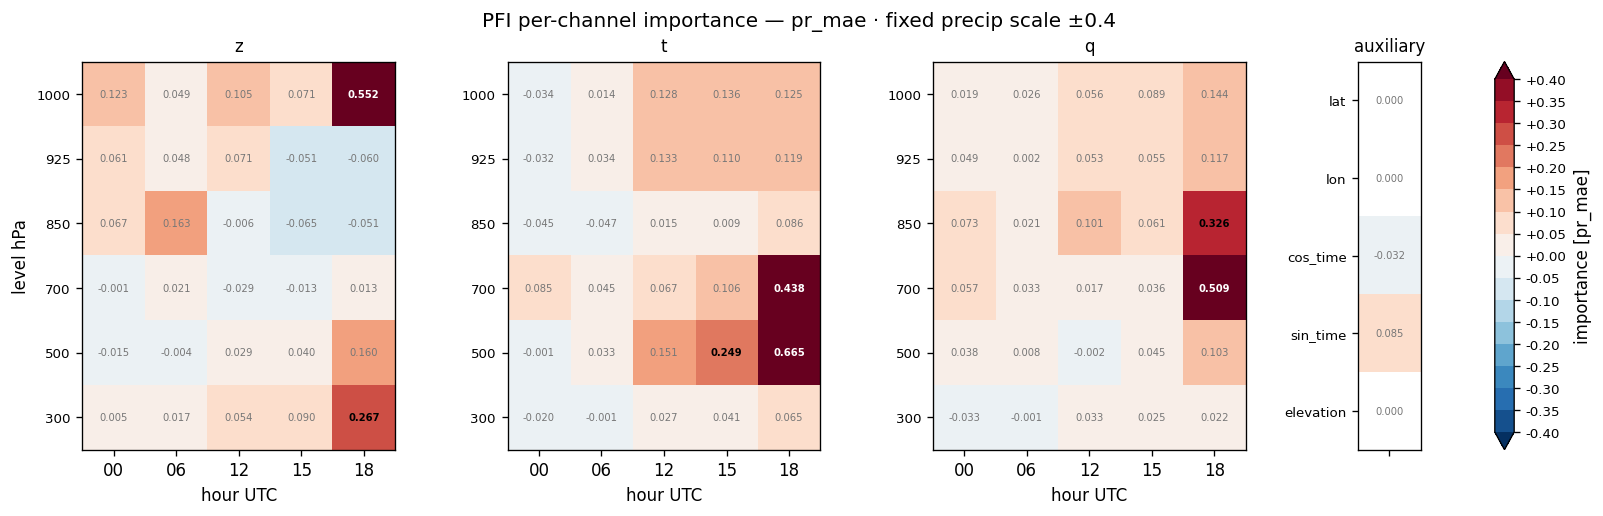
\includegraphics[width=0.84\textwidth,height=3.9cm,keepaspectratio]{images/results/precip__pfi_heatmap_pr_mae__feature_importance_2024__clean_solo_precip_ftcrps.png}}\\[1ex]
\subfloat[Grouped LIME feature importance]{%
  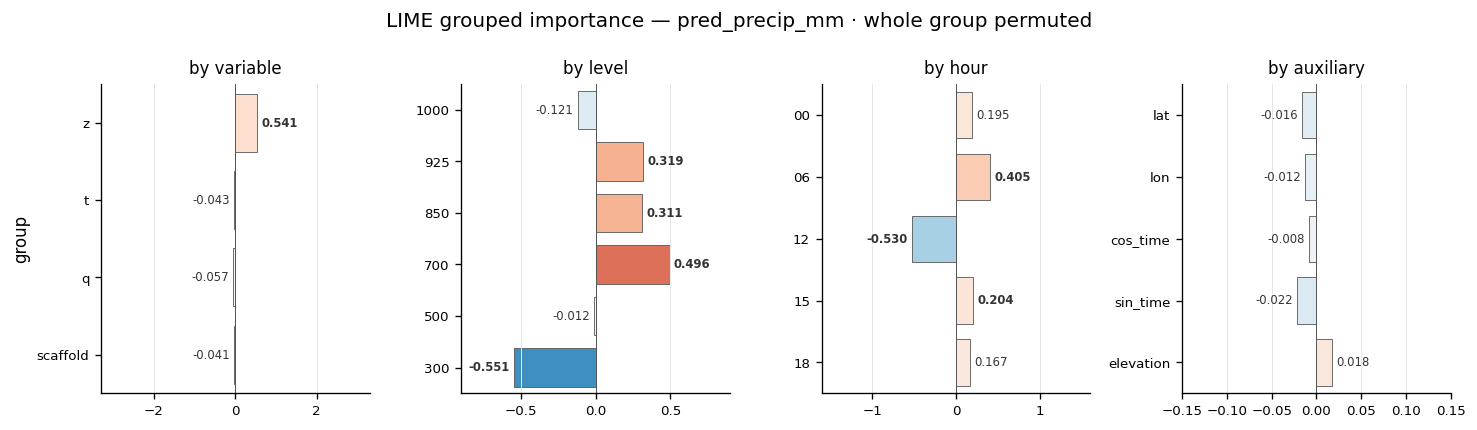
\includegraphics[width=0.84\textwidth,height=3.9cm,keepaspectratio]{images/results/precip__lime_groups_pred_precip_mm__feature_importance_2024__clean_solo_precip_ftcrps.png}}\\[1ex]
\subfloat[Per-channel LIME feature importance]{%
  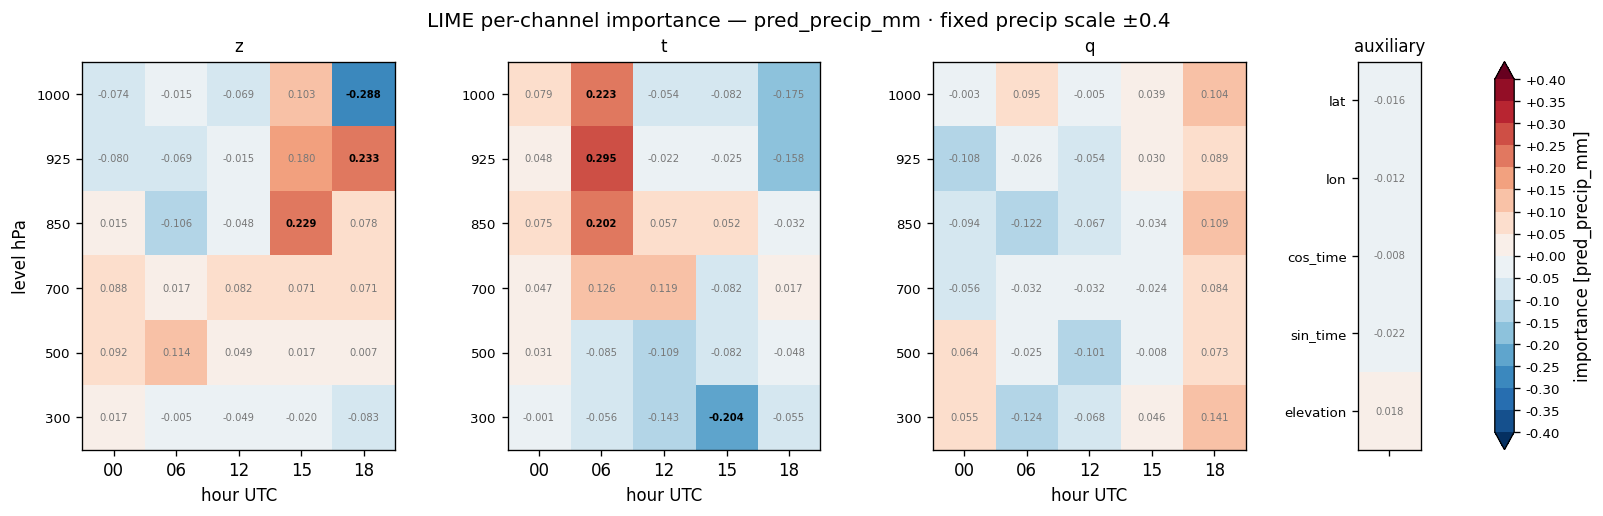
\includegraphics[width=0.84\textwidth,height=3.9cm,keepaspectratio]{images/results/precip__lime_heatmap_pred_precip_mm__feature_importance_2024__clean_solo_precip_ftcrps.png}}
\caption[Feature Importance of the selected atmospheric precipitation model]{Feature Importance of \texttt{precip-FT-CRPS}, the selected atmospheric precipitation model, in
millimetres. The grouped permutation view puts specific humidity far ahead of temperature and
geopotential and 06~UTC ahead of the other hours. LIME does not reproduce that ordering, which is
discussed in \sref{subsec:app-fi-lime}; for precipitation the permutation result is the one carried
forward.}
\label{fig:app-fi-sel-precip-ft}
\end{figure}

\begin{figure}[p]
\centering
% This model has seven channels and no levels or hours, so its panels are near-square
% rather than the 3:1 of the atmospheric runs: 2x2 uses the page, 4x1 does not.
\subfloat[Grouped permutation importance]{%
  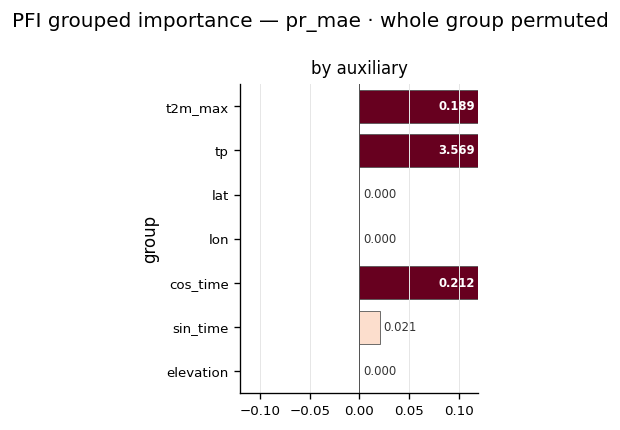
\includegraphics[width=0.47\textwidth,height=5.0cm,keepaspectratio]{images/results/precip__pfi_groups_pr_mae__feature_importance_2024__clean_solo_precip_sfctp.png}}\hfill
\subfloat[Grouped LIME feature importance]{%
  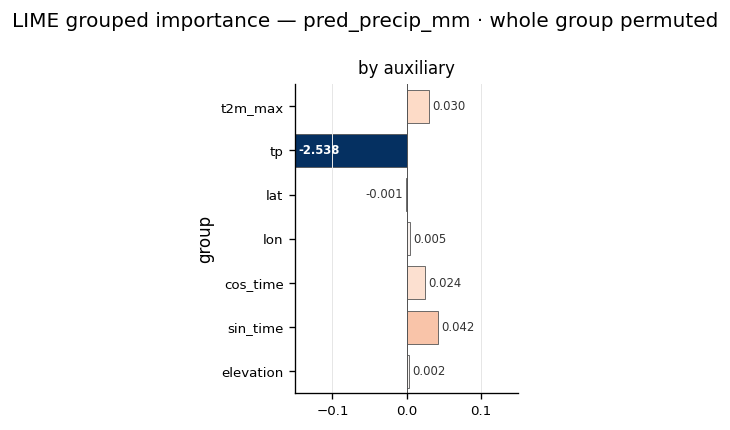
\includegraphics[width=0.47\textwidth,height=5.0cm,keepaspectratio]{images/results/precip__lime_groups_pred_precip_mm__feature_importance_2024__clean_solo_precip_sfctp.png}}\\[1ex]
\subfloat[Per-channel permutation importance]{%
  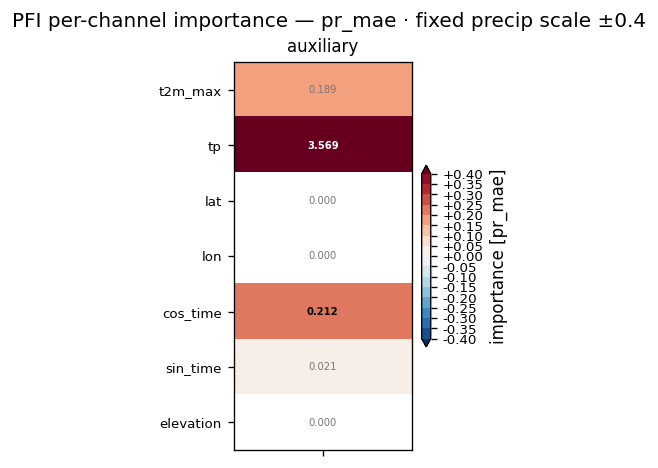
\includegraphics[width=0.47\textwidth,height=5.0cm,keepaspectratio]{images/results/precip__pfi_heatmap_pr_mae__feature_importance_2024__clean_solo_precip_sfctp.png}}\hfill
\subfloat[Per-channel LIME feature importance]{%
  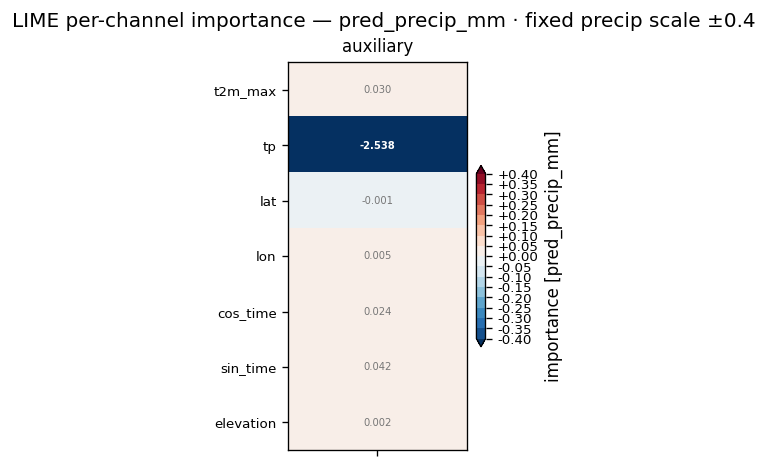
\includegraphics[width=0.47\textwidth,height=5.0cm,keepaspectratio]{images/results/precip__lime_heatmap_pred_precip_mm__feature_importance_2024__clean_solo_precip_sfctp.png}}
\caption[Feature Importance of the selected surface precipitation model]{Feature Importance of \texttt{precip-SFC-TP}, the selected surface precipitation model, in
millimetres. With no pressure levels or sampling hours to group by, the grouping collapses to the
seven channels themselves. Permutation gives the coarse \texttt{tp} accumulation almost the whole of
the model's importance; LIME gives the same channel a large negative coefficient, which is the
clearest illustration of the sign caveat in \sref{subsec:app-fi-lime}.}
\label{fig:app-fi-sel-precip-sfc}
\end{figure}

\FloatBarrier
\subsection{All Configurations at a Glance}\label{subsec:app-fi-allmodels}

Rather than one figure per configuration, every model of a variable is placed in a single figure per
method. One property of these figures has to be read before their bars: each bar is a \emph{share of
that model's largest group in the panel}, and the labelled bar carries the absolute value it was
scaled by. Bar lengths are therefore comparable \emph{within} a model and not between models, which
is the opposite convention to every other importance figure in this work. This normalisation is
required to make the comparison possible at all, since the surface models carry their whole importance in one
channel while the atmospheric models spread it over ninety or, with wind, a hundred and fifty.

The precipitation permutation view is not repeated here: it is
\fref{fig:single-precip-fi} in the main text.

\begin{figure}[h]
\centering
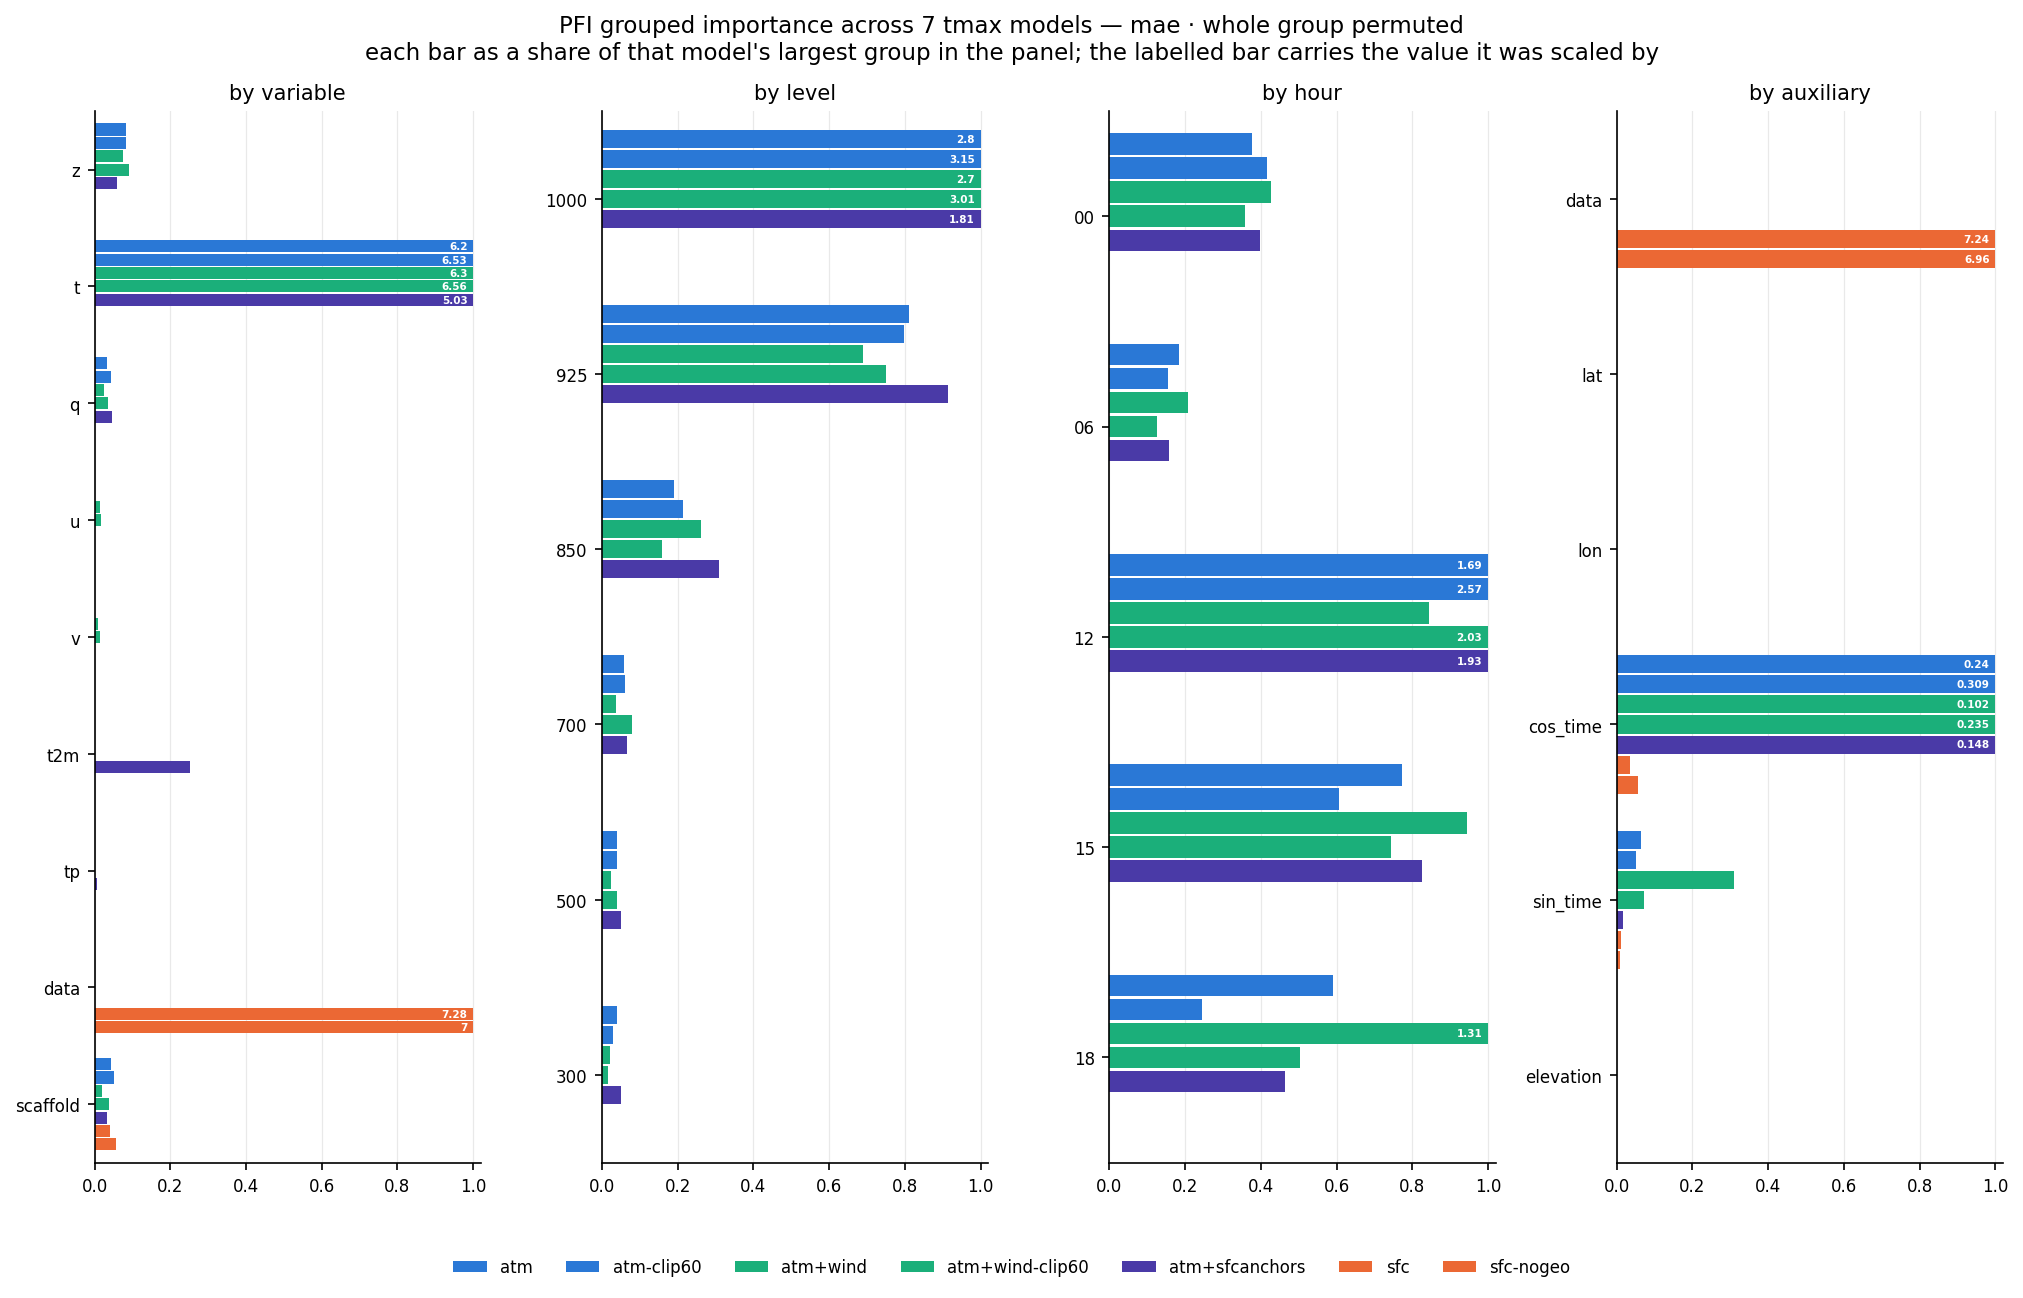
\includegraphics[width=\textwidth]{images/results/tmax__fi_group_importance_pfi_2024__tmax_model_comparison__ALL.png}
\caption[Grouped permutation importance across all temperature models]{Grouped permutation
importance of all seven temperature configurations, on the 2024 holdout. Each bar is a share of that
model's largest group in its panel and the labelled bars carry the degrees Celsius they were scaled
by, so the panels compare the \emph{shape} of a model's reliance rather than its magnitude. The two
surface models put everything into their single data channel; the five atmospheric ones agree on
temperature over geopotential and humidity, on $1000$ and $925\,\mathrm{hPa}$ over the levels above,
and on the midday and afternoon hours, with the wind groups $u$ and $v$ negligible in both runs that
carry them.}
\label{fig:app-fi-all-tmax-pfi}
\end{figure}

\begin{figure}[h]
\centering
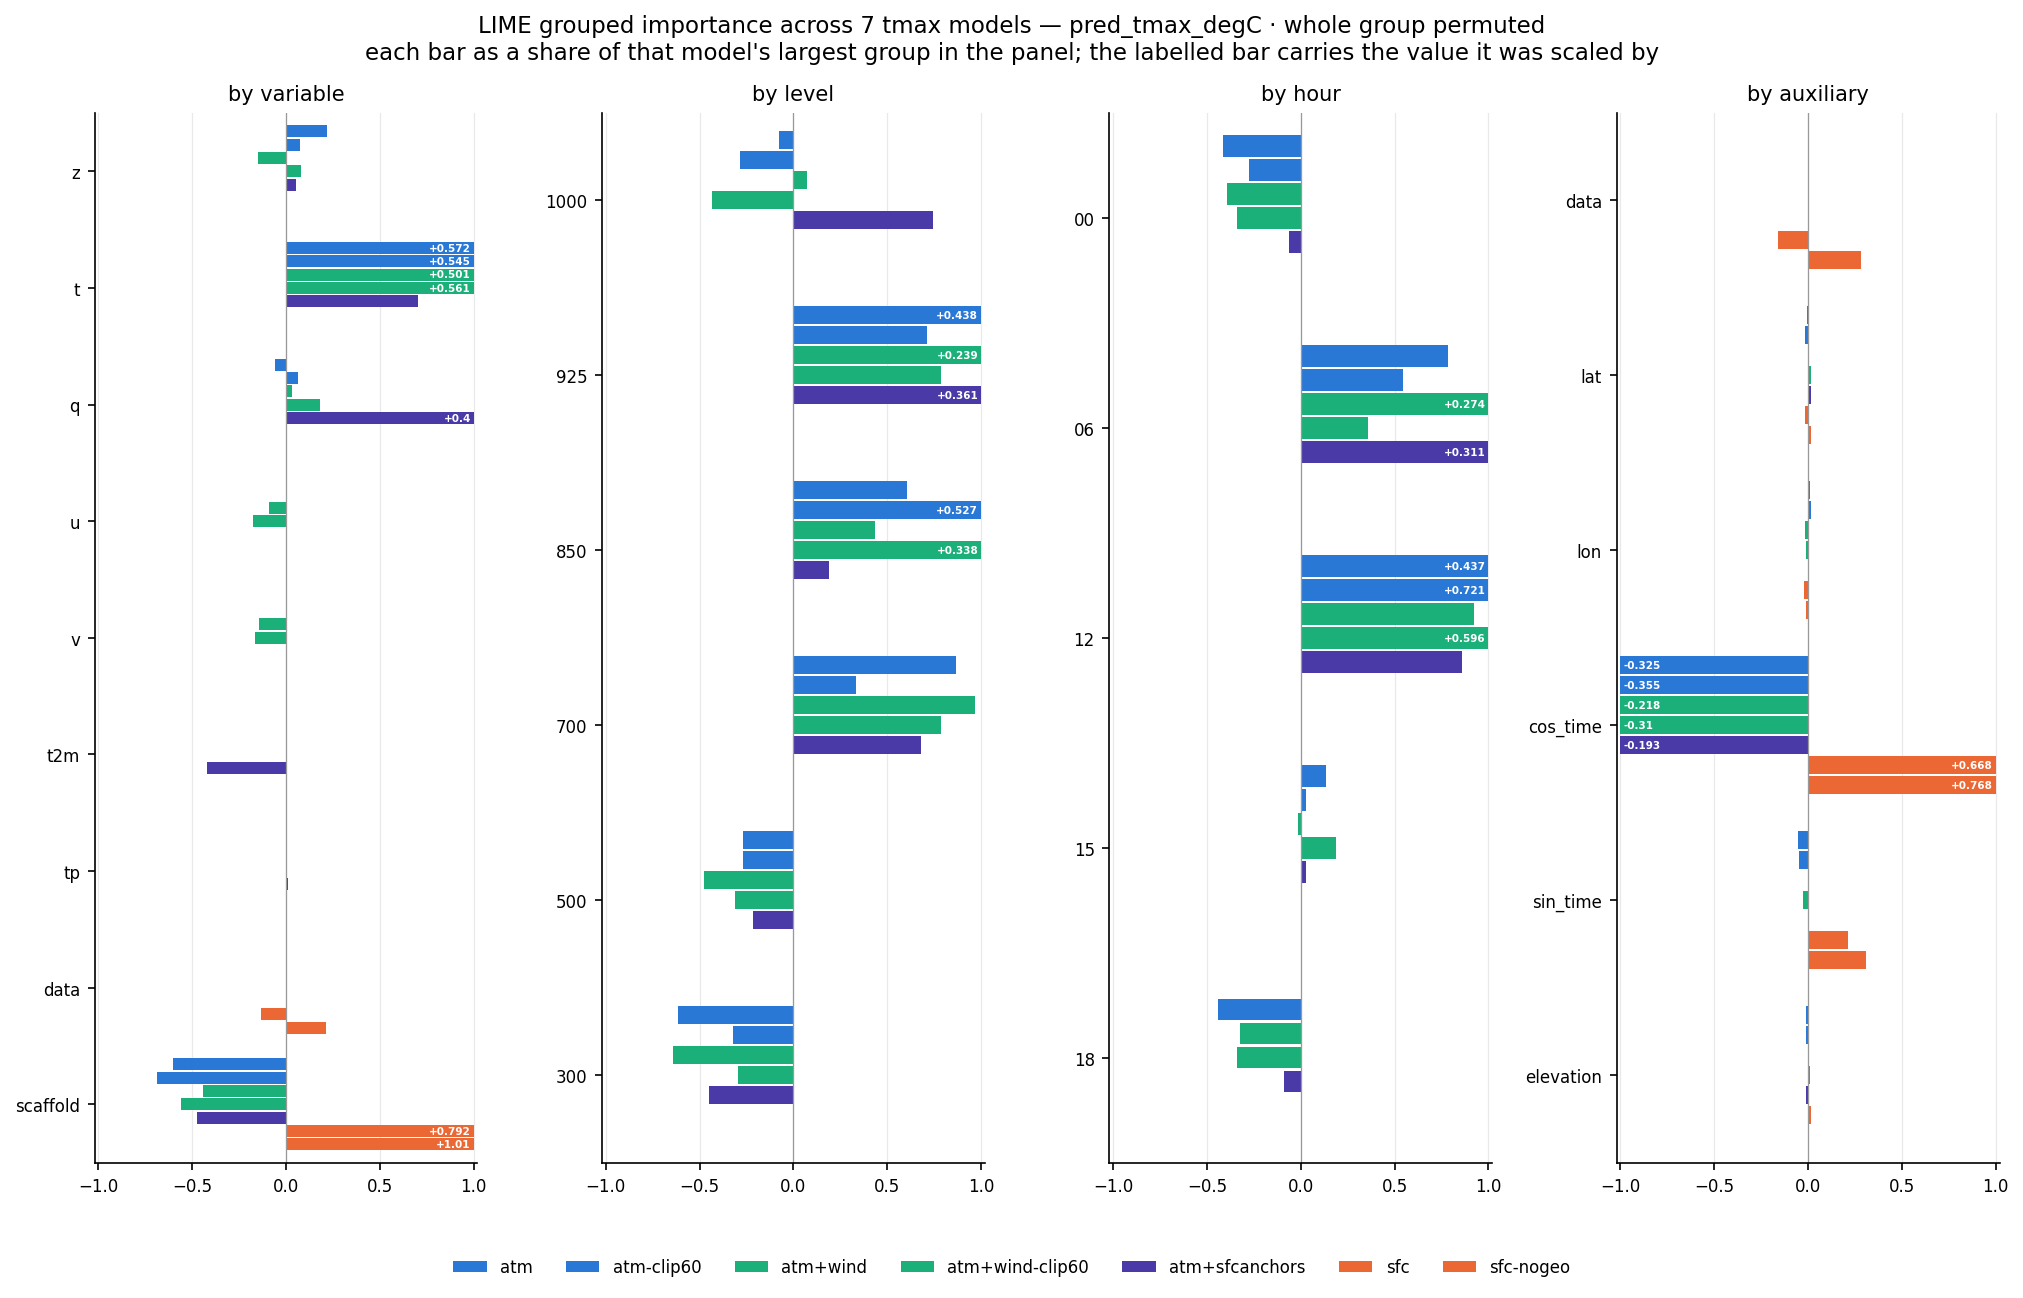
\includegraphics[width=\textwidth]{images/results/tmax__fi_group_importance_lime_2024__tmax_model_comparison__ALL.png}
\caption[Grouped LIME feature importance across all temperature models]{Grouped LIME feature
importance of all seven temperature configurations, normalised as in
\fref{fig:app-fi-all-tmax-pfi}. LIME reports a
signed effect on the spatial-mean prediction, so a bar may point either way and a negative one is a
direction rather than an absence of importance (\sref{subsec:app-fi-lime}).}
\label{fig:app-fi-all-tmax-lime}
\end{figure}

\begin{figure}[h]
\centering
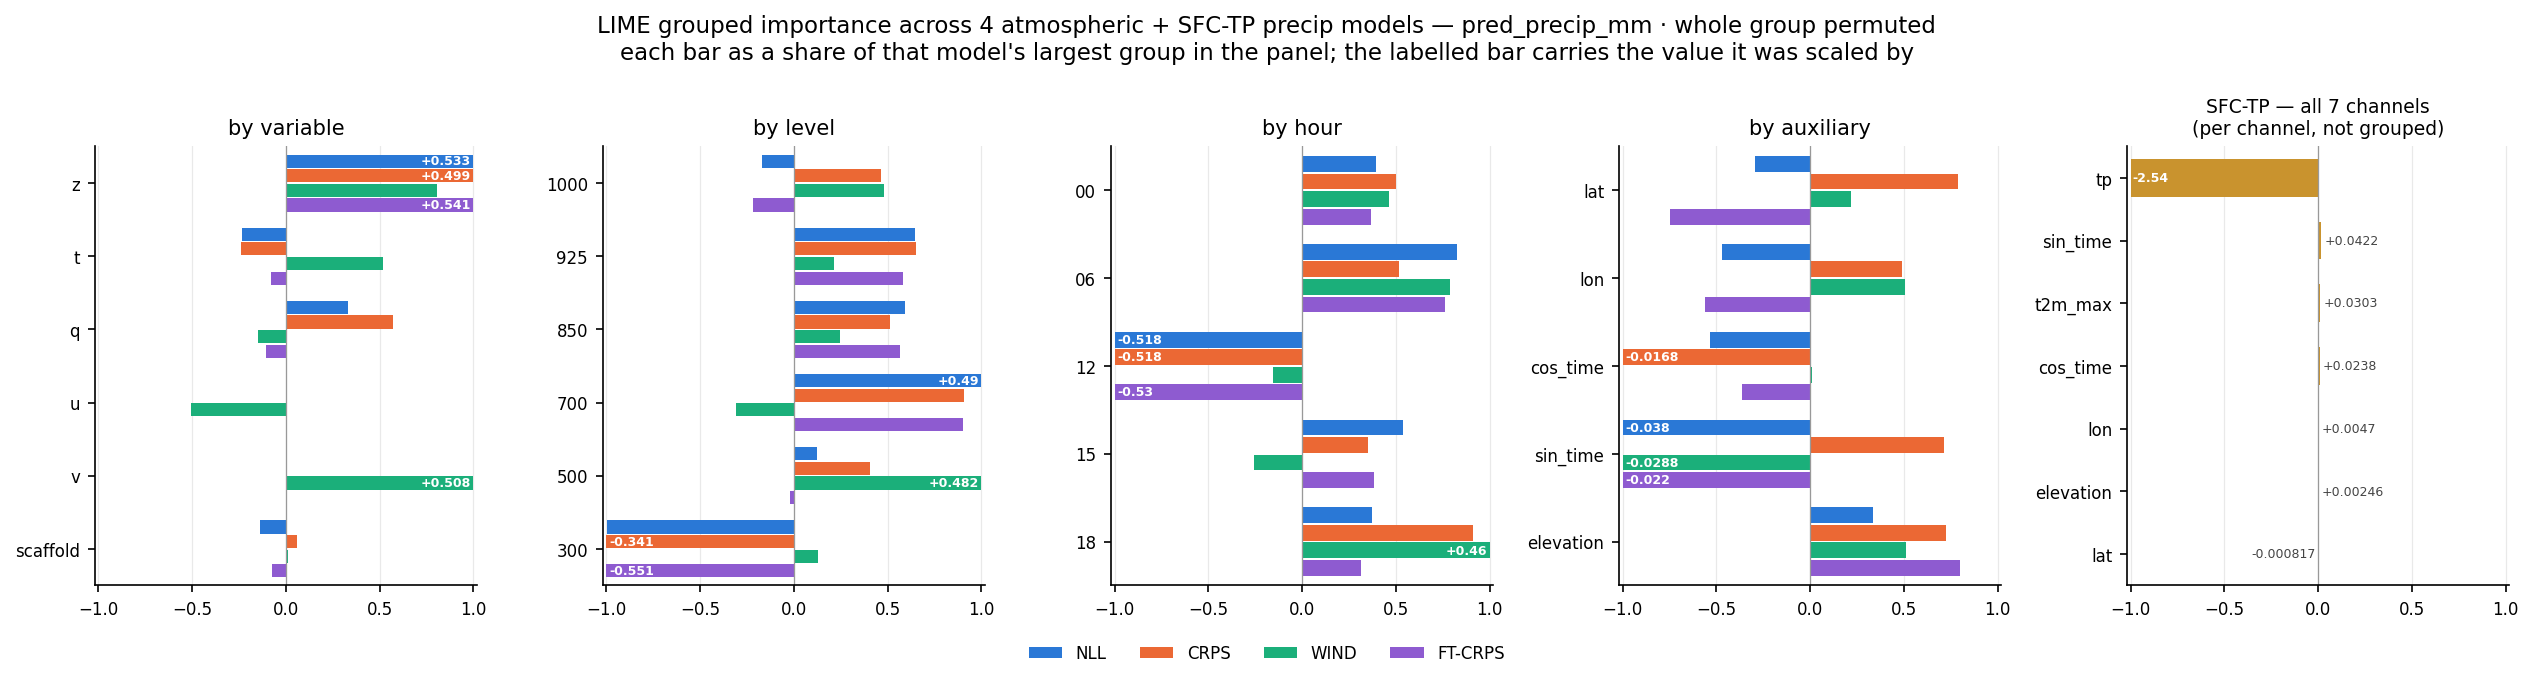
\includegraphics[width=\textwidth]{images/results/precip__fi_group_importance_lime_2024__precip_processing_comparison__ALL.png}
\caption[Grouped LIME feature importance across all precipitation models]{Grouped LIME feature
importance of all five precipitation configurations, normalised as in
\fref{fig:app-fi-all-tmax-pfi}. The permutation
counterpart is \fref{fig:single-precip-fi} in the main text. The disagreement between the two
methods on precipitation is the subject of \sref{subsec:app-fi-lime}.}
\label{fig:app-fi-all-precip-lime}
\end{figure}

\FloatBarrier
\subsection{Limitations of the Permutation Estimator}\label{subsec:app-fi-limits}

Four limitations bound what the importances reported in this work can support.
\begin{itemize}
\item \emph{Static channels are invisible.} Permuting along the day axis leaves a time-invariant
channel unchanged, so latitude, longitude and the coarse elevation score exactly zero by
construction. This is a property of the estimator, not a statement about the model, whose terrain
dependence is carried by the elevation MLP of \sref{subsec:meth-elev-mlp}.
\item \emph{Permutation forces extrapolation.} Pairing a January field with a July target day never
occurs in nature, so part of what is measured is a model queried outside its training
distribution~\cite{hooker2021unrestricted}. Grouping reduces this; only retraining would remove it.
\item \emph{The result describes this model, not the atmosphere.} A low importance means the fitted
model does not depend on that channel, not that the predictor is uninformative.
\item \emph{A shared scale is not a shared verdict.} Importances from different runs can be placed
on one axis, but a model spreading its reliance thinly is not for that reason worse than one leaning
on a few channels.
\end{itemize}

\subsection{The LIME Cross-Check}\label{subsec:app-fi-lime}

LIME explains one prediction by fitting a simple surrogate in a neighbourhood of
it~\cite{ribeiro2016lime}. The neighbourhood used here is built from the presence or absence of
input channels. For a chosen day a thousand binary masks are drawn over the channels; a masked
channel is replaced by its temporal-mean field, so it loses that day's anomaly while keeping its
spatial climatology and the field stays plausible. Each masked context is passed through the
five-fold ensemble and reduced to its spatial-mean prediction, giving one number per mask, and a
weighted ridge regression of that number on the masks returns one signed coefficient per channel,
with masks closer to the unmasked input weighted more heavily. A group coefficient is the sum over
the group's channels. Four days spread through the scored year are explained this way; the bars are
their mean and the error bars their spread.

It is kept as a cross-check rather than as evidence, and the figures above show why. The
coefficients are signed, so they mix a channel's importance with the direction in which that day's
anomaly happened to push the prediction, which is how the surface model's one informative channel
acquires a large negative value. The spread across the four days exceeds the effect for most groups,
so four days cannot support a statement about a model. The spatial field is averaged away before the
surrogate is fitted, and a downscaling model exists to produce spatial structure, so a channel that
redistributes precipitation without changing the domain total is invisible to this target.
Permutation importance has no such bottleneck, because its metric is accumulated over every target
point. And the observations never enter, so LIME measures how strongly the prediction responds to a
channel rather than whether the channel makes the prediction better.

Where the two methods agree, which for temperature is the level of the variable families and the
leading hour, the agreement is worth having: they share nothing beyond the trained model, having a
different perturbation, a different target and a different estimator. Where they disagree, as they
do for precipitation, the permutation result is the one carried forward.

\begin{figure}[H]
\centering
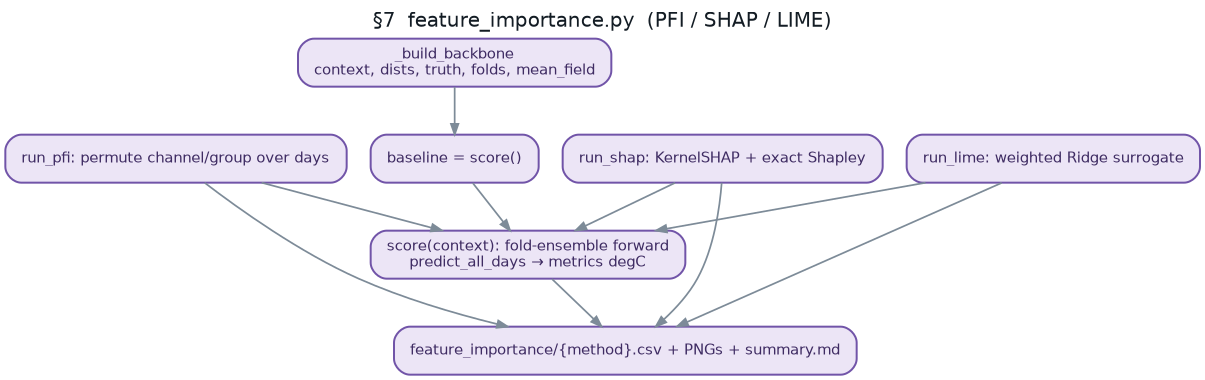
\includegraphics[width=\textwidth]{images/s7_feature_importance.png}
\caption[The feature-importance implementation]{Structure of the feature-importance implementation.
The three methods differ only in the perturbation they apply; all of them score through the same
fold-ensemble forward pass, so the model is treated as a black box throughout.}
\label{fig:app-fi-pipeline}
\end{figure}

\FloatBarrier
\section{Training Curves of the Precipitation Runs}\label{sec:app-precip-training}

The five runs of \tref{tab:single-precip-variants} minimise two different objectives, so the loss
each one descends is not the same quantity: three runs minimise the Bernoulli--Gamma likelihood of
\eref{eq:bg-ll}, \texttt{precip-CRPS} the sampled CRPS of \eref{eq:crps}, and
\texttt{precip-FT-CRPS} the second after converging on the first. The left panel of
\fref{fig:app-precip-training} therefore shows convergence only, each run on its own scale, and
nothing in it may be read as a ranking. The right panel is the one common criterion: the held-out
Bernoulli--Gamma CRPS, which every run reports whatever it was trained on, and which the
fine-tuning stops on.

Read on that criterion, \texttt{precip-FT-CRPS} reaches $1.762$ at its fourth fine-tune epoch
against $1.789$ at epoch $26$ for \texttt{precip-NLL} and $1.832$ at epoch $29$ for
\texttt{precip-CRPS}. A ten-epoch fine-tune budget from a converged likelihood model, ended by early stopping after
four to eight epochs, recovers more of the CRPS than thirty epochs of training on the CRPS from
scratch, which is the evidence behind the fine-tuned
variant being a third run rather than a variation of the second (\sref{objective}). Everything beyond convergence (accuracy,
occurrence, intensity and skill) is a result and is reported in
\sref{subsec:single-precip-headline}, not read off these curves.

\begin{figure}[H]
\centering
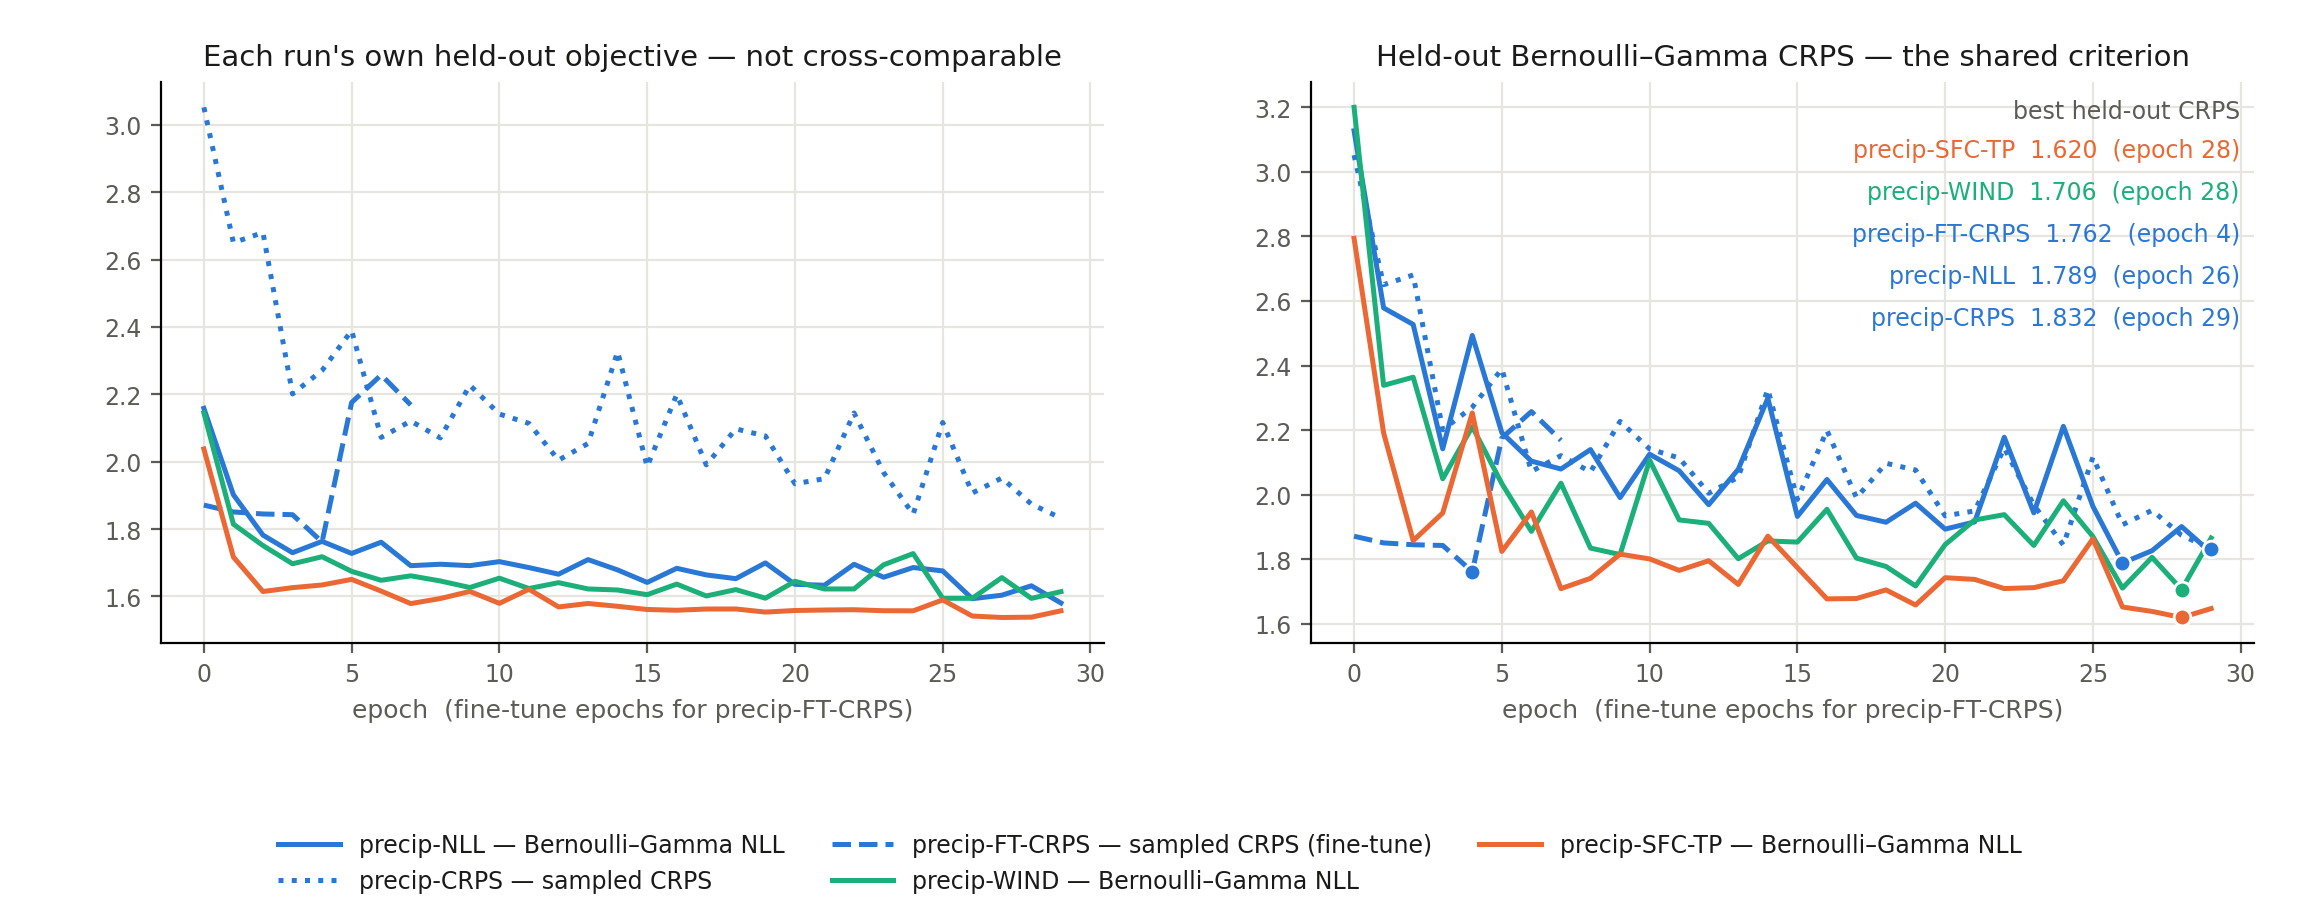
\includegraphics[width=\textwidth]{images/precip_training_curves.png}
\caption[Training curves of the precipitation runs]{Fold-averaged held-out training curves of the
five precipitation runs, on the colour and line-style conventions of
\fref{fig:single-precip-slope}. Left: each run's own objective, which for the two CRPS-trained runs
is the sampled CRPS and for the other three the Bernoulli--Gamma likelihood; the curves converge
but are not comparable to each other. Right: the held-out Bernoulli--Gamma CRPS, the single score
every run shares, with the best epoch marked on each curve. \texttt{precip-FT-CRPS} contributes only
its fine-tune epochs (a ten-epoch budget ended by early stopping), which begin from the converged \texttt{precip-NLL} model, so its epoch
axis counts epochs after the warm start and is not comparable to the from-scratch runs.}
\label{fig:app-precip-training}
\end{figure}

\FloatBarrier
\section{Spatial Intensity Categories for the Remaining Precipitation Runs}\label{sec:app-precip-category-spatial}

\fref{fig:single-precip-spatial-categories} compares \texttt{precip-FT-CRPS} and
\texttt{precip-SFC-TP}, the two runs selected in \sref{subsec:single-precip-selection}. The three
remaining runs are reproduced here on the same five intensity categories, each against the observed
field and the bilinear ERA5-Land reference, with its own Brier skill. Unlike the main-text figure,
these are the per-run renderings, so the frequency colour scale is chosen per figure rather than
shared across runs: read them for pattern and for the skill columns, not for colour-matched
comparison between runs.

\begin{figure}[H]
\centering
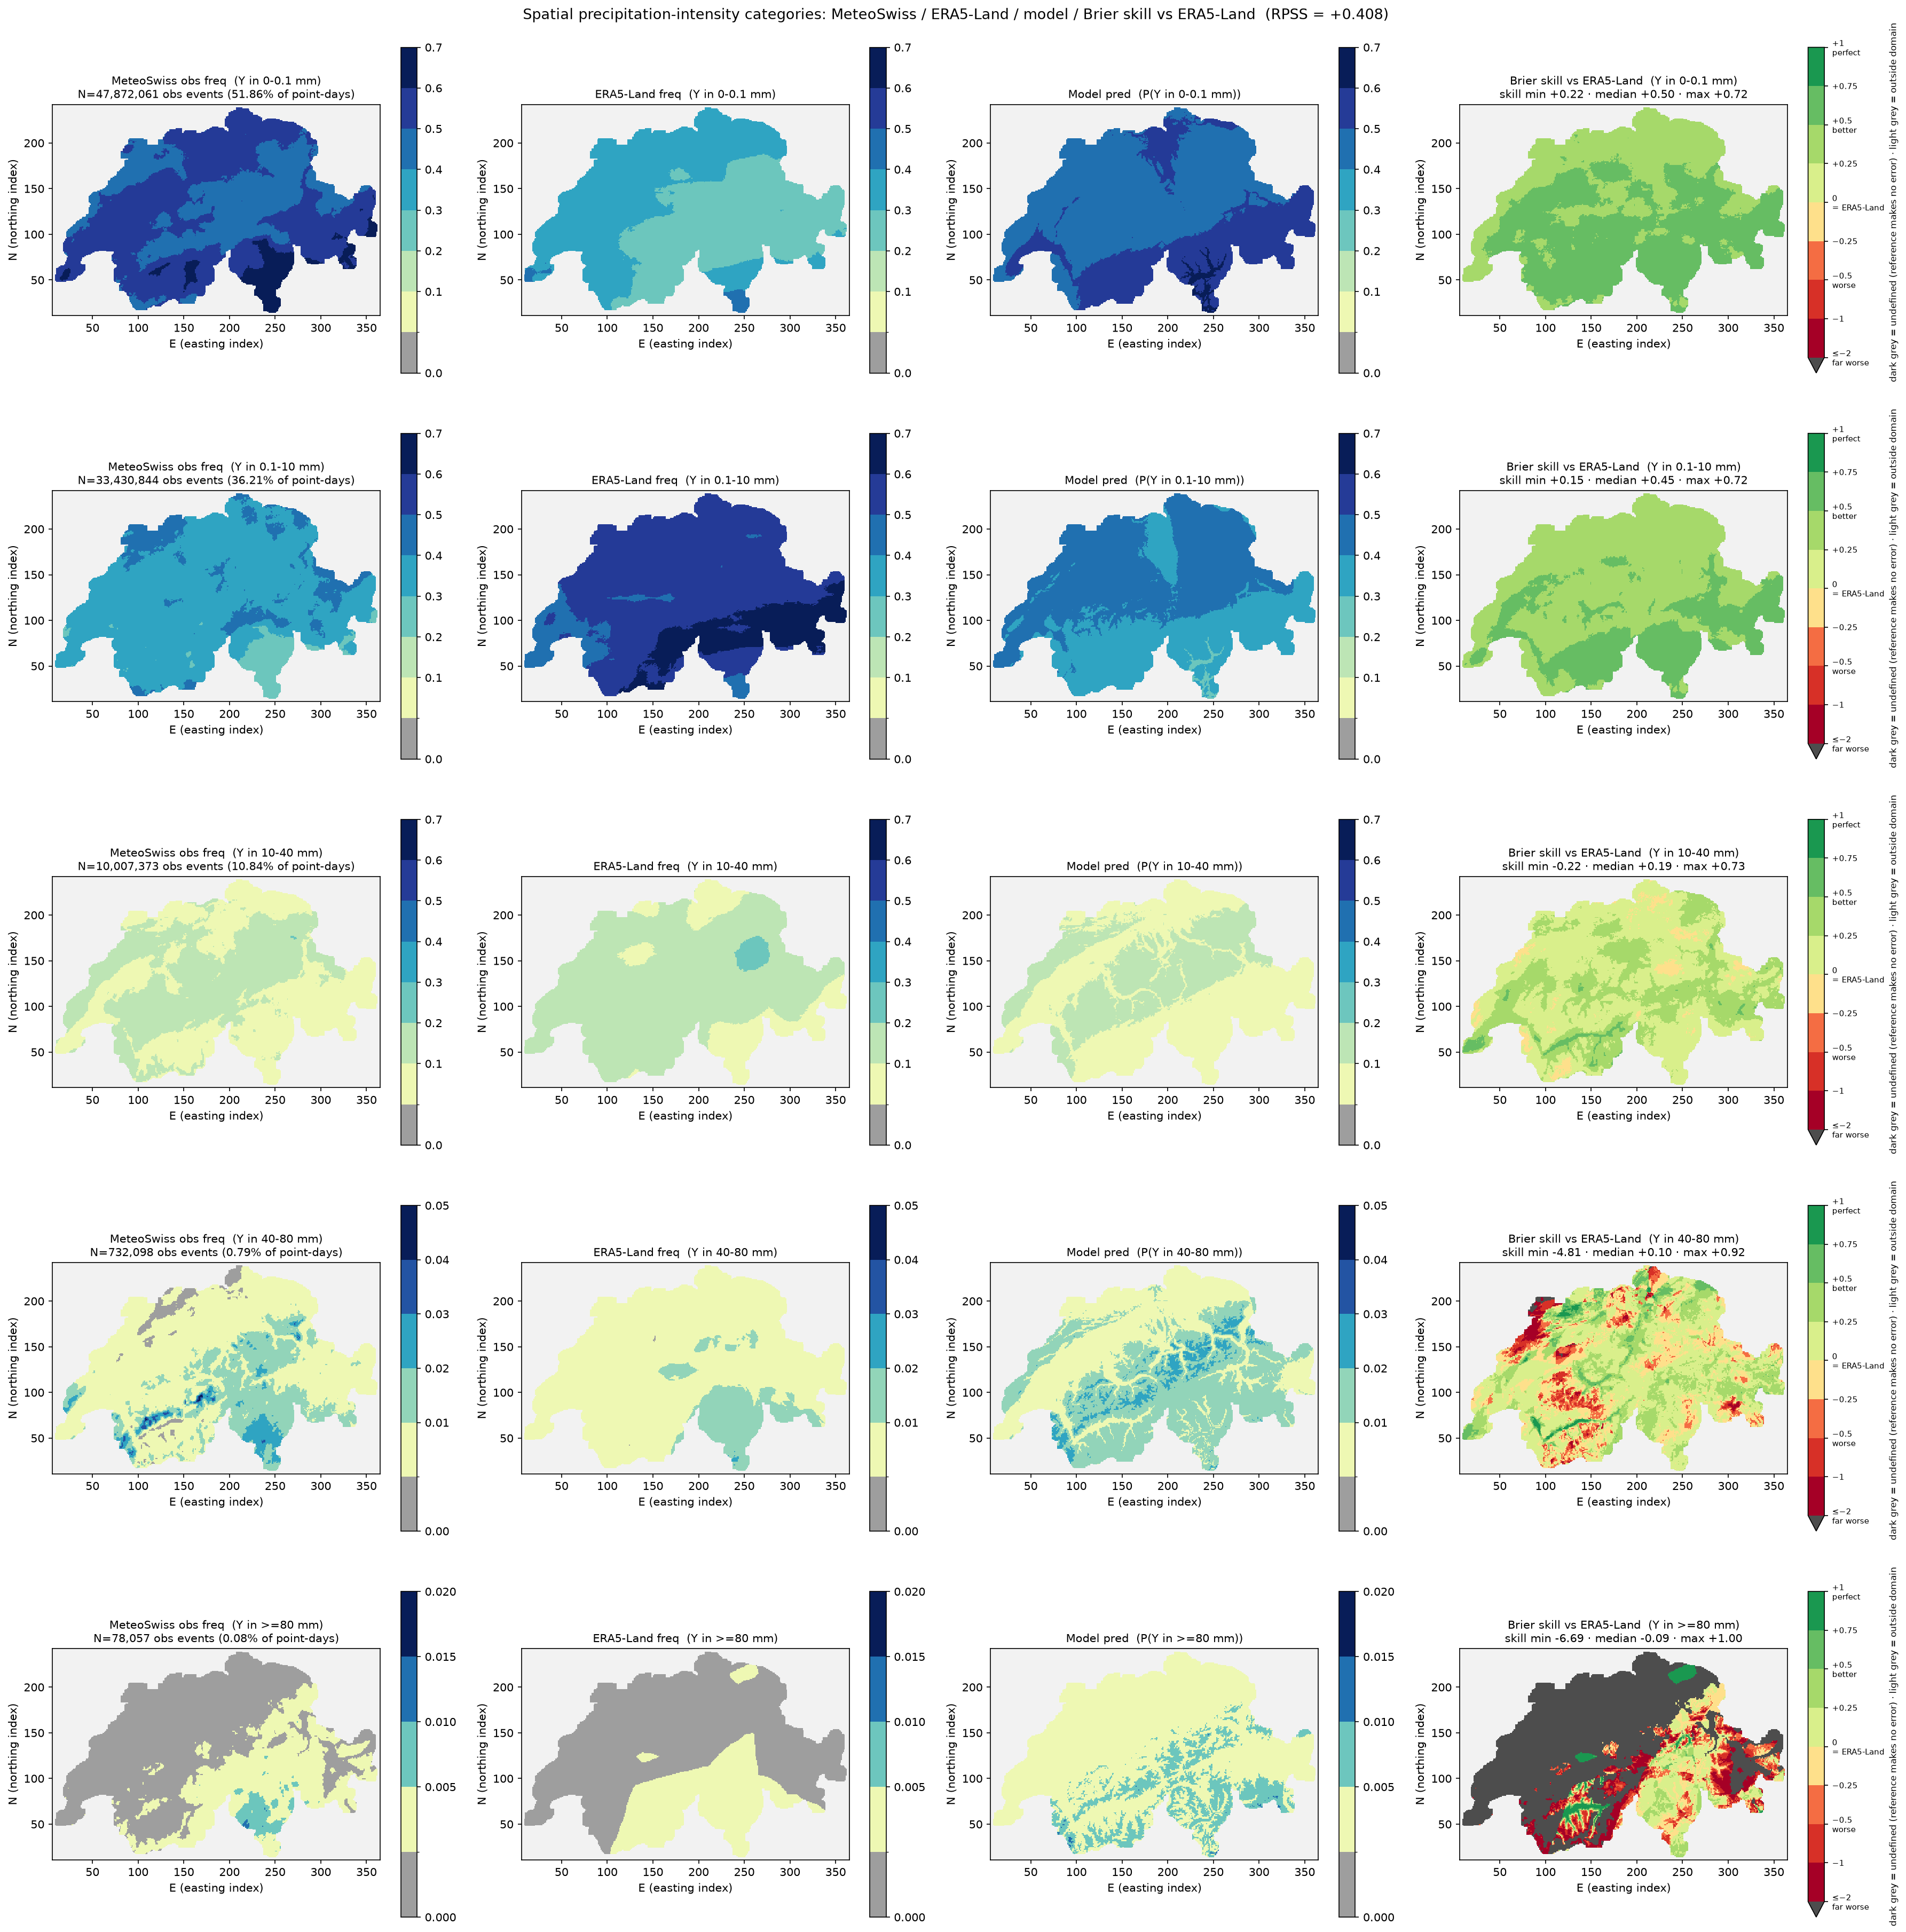
\includegraphics[width=0.92\textwidth]{images/results/precip__precip_category_spatial__eval_cv__clean_solo_precip.png}
\caption[Spatial intensity categories, \texttt{precip-NLL}]{\texttt{precip-NLL} on the CV holdout.
This is the run the naive reference beats on the tail (\sref{subsec:single-precip-headline}), and
the $\geq 80\,\mathrm{mm}$ skill column is correspondingly the weakest of the five.}
\label{fig:app-precip-catspatial-nll}
\end{figure}

\begin{figure}[H]
\centering
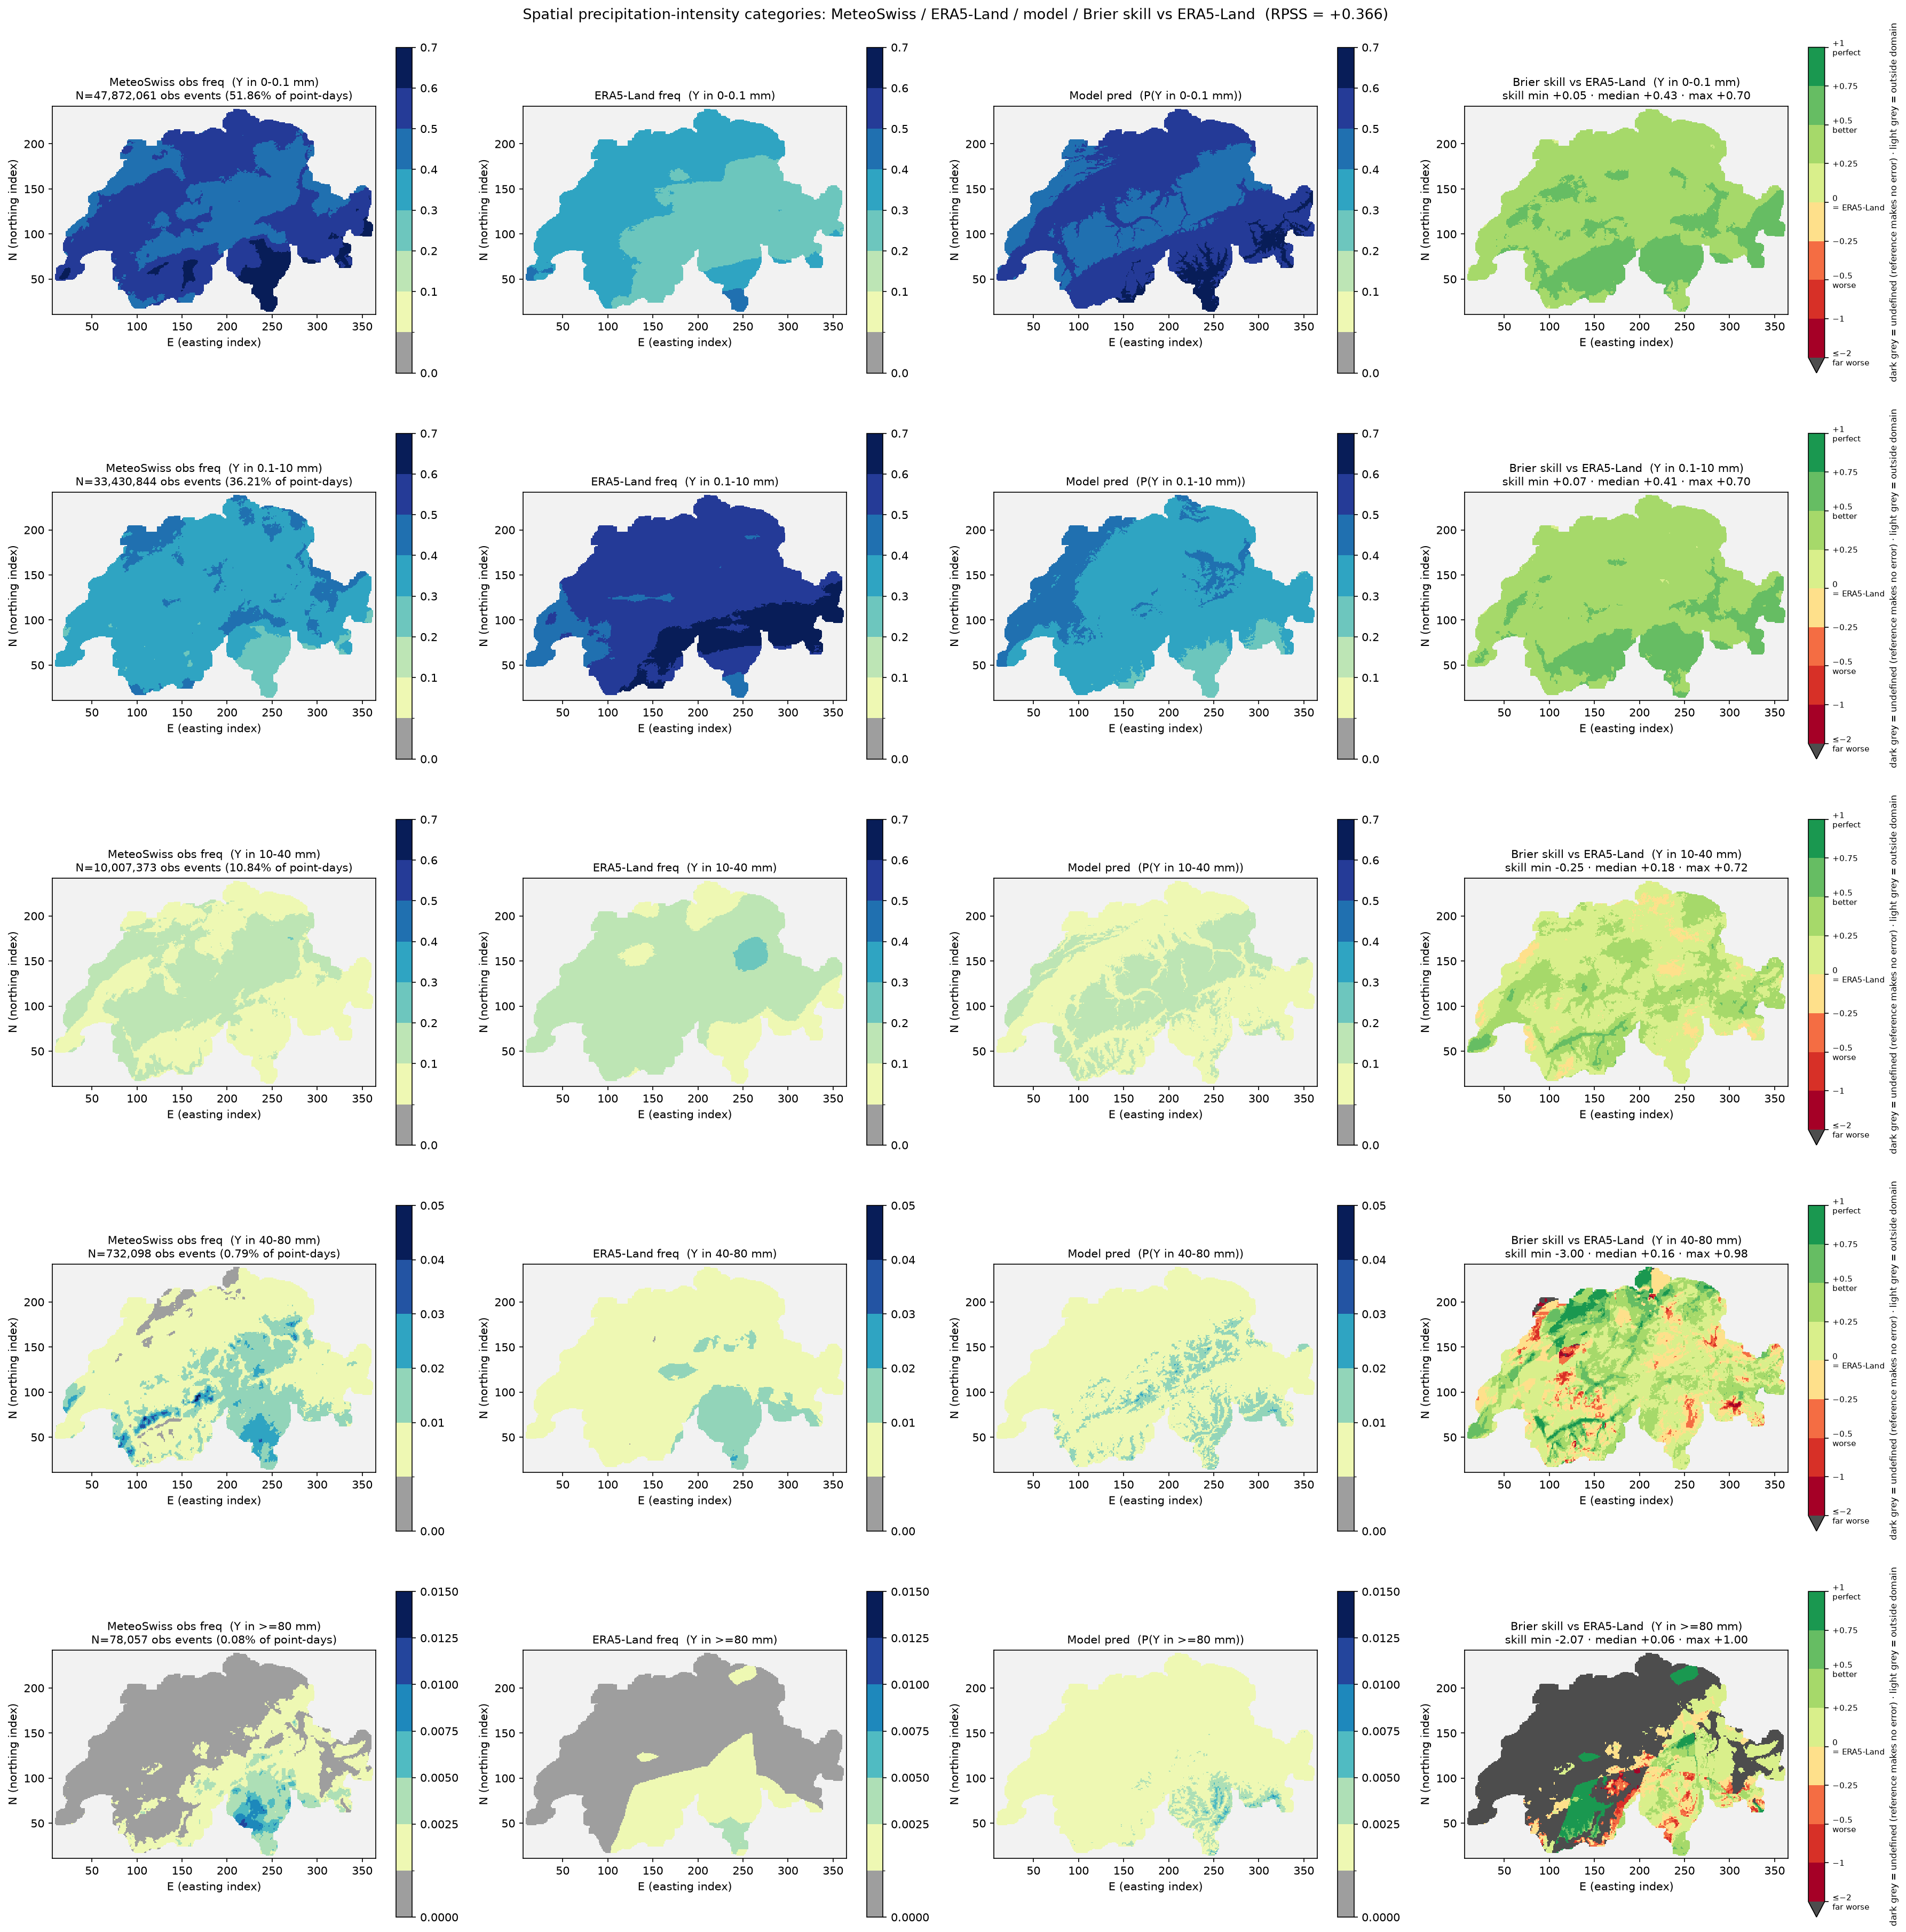
\includegraphics[width=0.92\textwidth]{images/results/precip__precip_category_spatial__eval_cv__clean_solo_precip_crps.png}
\caption[Spatial intensity categories, \texttt{precip-CRPS}]{\texttt{precip-CRPS} on the CV
holdout. The driest of the objectives and the best of the five in the heaviest category on this
regime, bought by being the weakest of the five in the two categories that hold most of the days
(\sref{subsec:single-precip-categories}).}
\label{fig:app-precip-catspatial-crps}
\end{figure}

\begin{figure}[H]
\centering
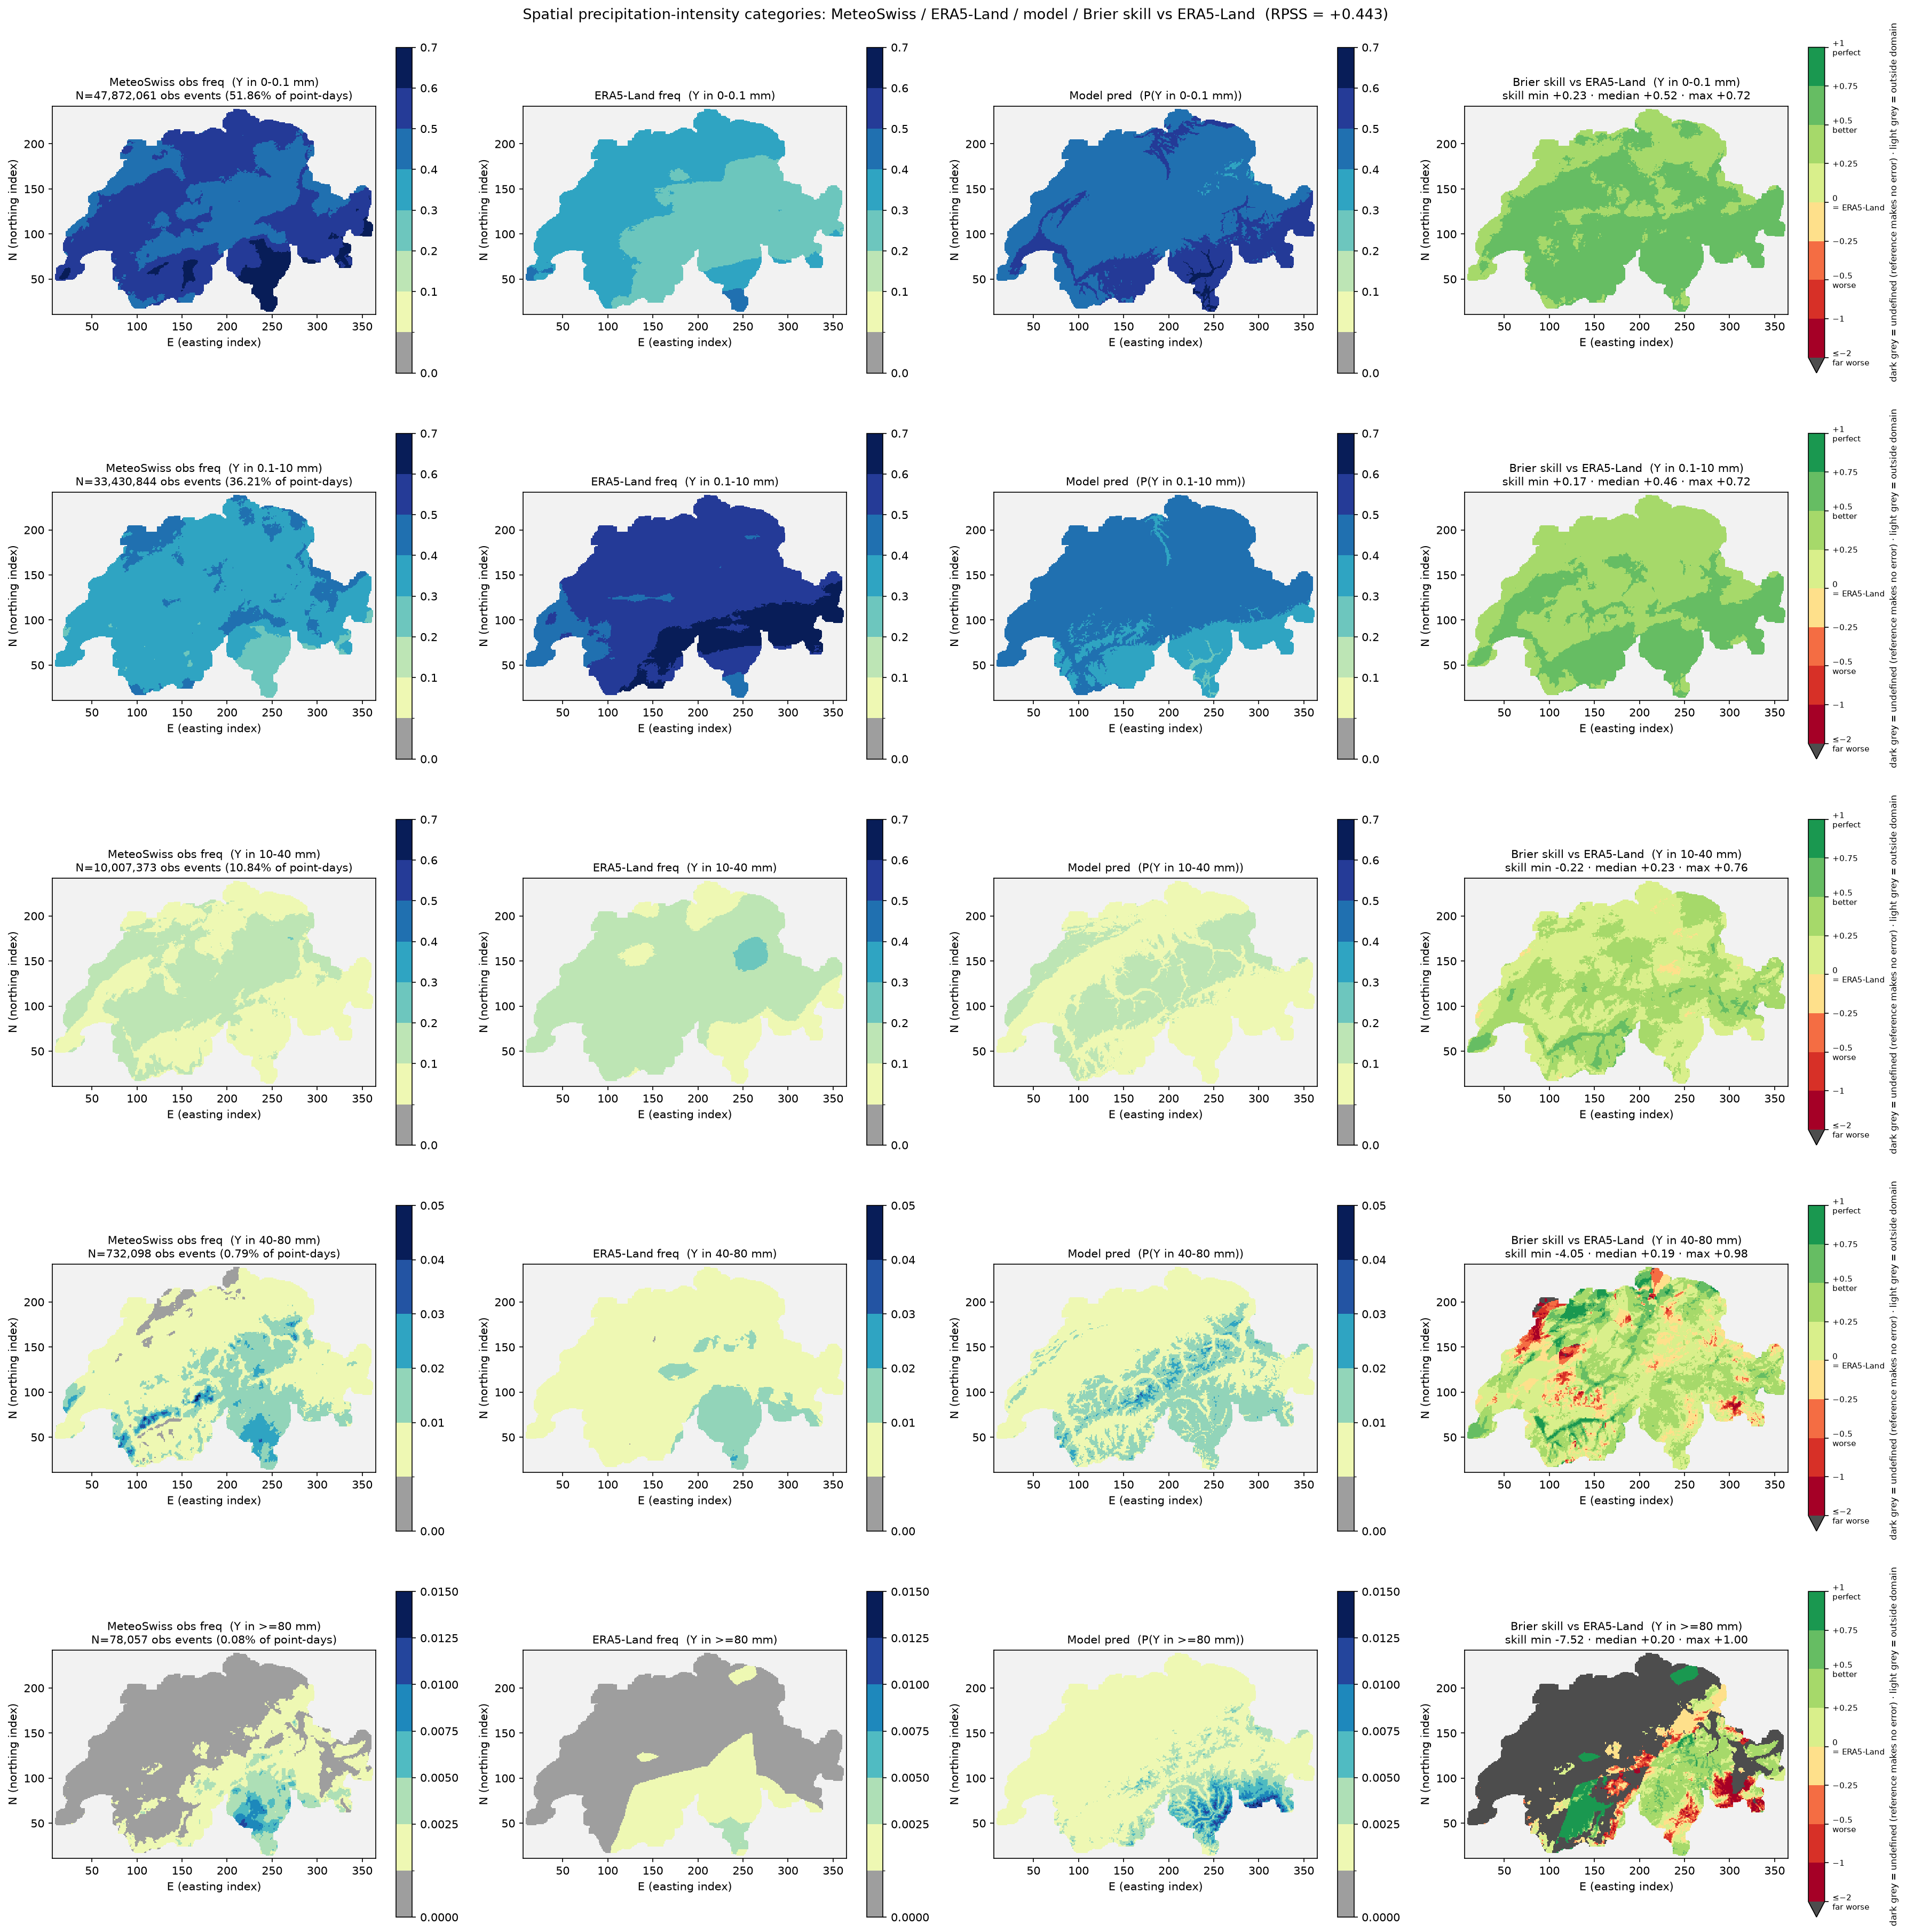
\includegraphics[width=0.92\textwidth]{images/results/precip__precip_category_spatial__eval_cv__clean_solo_precip_wind.png}
\caption[Spatial intensity categories, \texttt{precip-WIND}]{\texttt{precip-WIND} on the CV
holdout, the strongest of the four atmospheric runs on both pooled skill scores
(\tref{tab:single-precip-selection}). Its lead is spread evenly over the first three categories
rather than concentrated anywhere, which is why it does not show as a distinct spatial pattern.}
\label{fig:app-precip-catspatial-wind}
\end{figure}

\section{Station Verification Details}\label{sec:app-stations}

This section carries the data statement behind \cref{ch:stations}: how the three station sets were
selected and checked. A station enters its set if it reports on at least $95\,\%$ of the days in 2020--2024, and is scored
only where enough valid days remain ($10$ for temperature, $30$ for the per-gauge precipitation
scores). The SMN metadata lists $158$ stations, of which $8$ deliver no data in the study window; $149$
report temperature and $139$ operate a rain gauge. The coverage cut removes two temperature
series and no gauge, leaving the $147$ temperature stations and $139$ gauges of
\tref{tab:stations-sets}. The gauge observable is the $06$--$06\,\mathrm{UTC}$ daily
total, the accumulation window RhiresD itself uses \cite{meteoswiss_rhiresd_doc}. The SMN series are operational rather than
homogenised; at the $28$ sites present in both temperature sets, the operational and the homogenised
NBCN series give per-station MAEs identical to a median of $0.00\,^{\circ}\mathrm{C}$ (maximum
difference $0.08\,^{\circ}\mathrm{C}$), so the distinction carries no weight over this span.

\end{document}

